% BEGIN LICENSE BLOCK
% Version: CMPL 1.1
%
% The contents of this file are subject to the Cisco-style Mozilla Public
% License Version 1.1 (the "License"); you may not use this file except
% in compliance with the License.  You may obtain a copy of the License
% at www.eclipse-clp.org/license.
% 
% Software distributed under the License is distributed on an "AS IS"
% basis, WITHOUT WARRANTY OF ANY KIND, either express or implied.  See
% the License for the specific language governing rights and limitations
% under the License. 
% 
% The Original Code is  The ECLiPSe Constraint Logic Programming System. 
% The Initial Developer of the Original Code is  Cisco Systems, Inc. 
% Portions created by the Initial Developer are
% Copyright (C) 1993 - 2006 Cisco Systems, Inc.  All Rights Reserved.
% 
% Contributor(s): 
% 
% END LICENSE BLOCK
%
%
% umsroot.tex
%--------------------------------------------------------------
%
% Root file for ECLiPSe User Manual, formerly SEPIA manual
%
%--------------------------------------------------------------

%\documentstyle[11pt,html,a4wide,epsf,alltt]{book}
\documentclass[11pt,a4paper]{book}
\usepackage{hevea}
\usepackage{alltt}
\usepackage{graphics}
%\usepackage{html}
\usepackage{epsf}
\usepackage{ae}
\usepackage{aecompl}
\usepackage{tocbibind}
\usepackage{makeidx}
\usepackage{hyperref}

\topmargin -1cm
\oddsidemargin 0cm
\evensidemargin 0cm
\textwidth 16cm
\textheight 22.5cm

\usepackage{../texinputs/eclipse}
%
% $Id: sepiachiphtml.tex,v 1.3 2008/06/19 18:06:21 jschimpf Exp $
%
% BEGIN LICENSE BLOCK
% Version: CMPL 1.1
%
% The contents of this file are subject to the Cisco-style Mozilla Public
% License Version 1.1 (the "License"); you may not use this file except
% in compliance with the License.  You may obtain a copy of the License
% at www.eclipse-clp.org/license.
% 
% Software distributed under the License is distributed on an "AS IS"
% basis, WITHOUT WARRANTY OF ANY KIND, either express or implied.  See
% the License for the specific language governing rights and limitations
% under the License. 
% 
% The Original Code is  The ECLiPSe Constraint Logic Programming System. 
% The Initial Developer of the Original Code is  Cisco Systems, Inc. 
% Portions created by the Initial Developer are
% Copyright (C) 2006 Cisco Systems, Inc.  All Rights Reserved.
% 
% Contributor(s): 
% 
% END LICENSE BLOCK

% This is not the original sepiachip.sty,
% but a drastically simplified one.
%

\newcommand{\eclipseversion}{6.0}


\newcommand{\newitem}[1]{\item[#1]}
\newcommand{\bipnoidx}[1]{{\bf #1}}
\newcommand{\bip}[1]{\bipnoidx{#1}\index{#1}}
%\newcommand{\biprefnoidx}[2]{\latex{{\bf #1}}\html{\htmladdnormallink{#1}{#2}}}
\newcommand{\biprefnoidx}[2]{\ahref{#2}{{\bf #1}}}
\newcommand{\bipref}[2]{\biprefnoidx{#1}{#2}\index{#1}}
\newcommand{\biptxt}[2]{\bipnoidx{#1}\index{#2}}
\newcommand{\txtbip}[2]{\bipnoidx{#1}\index{#1}}
\newcommand{\biptxtref}[3]{\biprefnoidx{#1}{#3}\index{#2}}
\newcommand{\txtbipref}[3]{\biprefnoidx{#1}{#3}\index{#1}}

% characters for indexing ? needed for a HeVeA bug
\newcommand{\query}{?}
\newcommand{\atsym}{@}

\newcommand{\vbar}{$\mid$}
\newcommand{\uparr}{$\wedge$}
\newcommand{\bsl}{$\backslash$}
\newcommand{\andsy}{$/\backslash$}
\newcommand{\orsy}{$\backslash/$}
\newcommand{\tld}{$\sim$}
\newcommand{\lbr}{$[$}
\newcommand{\rbr}{$]$}
\newcommand{\nil}{$[~]$}
\newcommand{\lt}{$<$}
\newcommand{\gt}{$>$}
\newcommand{\chr}{{\sf CHR}}
\newcommand{\chrs}{{\sf CHR}s}
\newcommand{\eclipse}{ECL$^i$PS$^e$}
\newcommand{\tkeclipse}{TkECL$^i$PS$^e$}
\newcommand{\sepia}{SEPIA}


\let\ifonline=\iffalse



%
% @(#)umsdebuggercomms.tex	1.3 93/03/29 
%
\newenvironment{descr}[1]
{\begin{list}{}{\setlength{\leftmargin}{#1}}}{\end{list}}
\def\cmd#1#2{\item[{\bf #1} \hfill] {\bf #2}\\
\index{#1 --- #2 (debugger cmd)}}
\def\ncmd#1#2{\item[{\it n\bf #1} \hfill] {\bf #2}\\
\index{#1 --- #2 (debugger cmd)}}
\def\mcmd#1#2{\item[{\bf #1 {\it par}} \hfill] {\bf #2}\\
\index{#1 --- #2 (debugger cmd)}}
\def\nmcmd#1#2{\item[{\it n\bf #1 {\it par}} \hfill] {\bf #2}\\
\index{#1 --- #2 (debugger cmd)}}

\title{
    {\Large\bf {\eclipse}}\\
    \vspace{1cm}
    {\Huge\bf User Manual}\\
    \vspace{1cm}
    Release \eclipseversion}


\author{
Abderrahamane Aggoun (ECRC) \\
David Chan (ECRC) \\
Pierre Dufresne (ECRC) \\
Eamon Falvey (ICL-ITC) \\
Hugh Grant (ICL-ITC) \\
Warwick Harvey (IC-Parc and CrossCore) \\
Alexander Herold (ECRC) \\
Geoffrey Macartney (ECRC) \\
Micha Meier (ECRC) \\
David Miller (ICL-ITC) \\
Shyam Mudambi (ECRC) \\
Stefano Novello (ECRC and IC-Parc) \\
Bruno Perez (ECRC) \\
Emmanuel van Rossum (ECRC) \\
Joachim Schimpf (ECRC, IC-Parc and CrossCore) \\
Kish Shen (IC-Parc and CrossCore)\\
Periklis Andreas Tsahageas (ECRC) \\
Dominique Henry de Villeneuve (ECRC) \\
}

%--------------------------------------------------------------

\makeindex

%--------------------------------------------------------------

\begin{document}


\nocite{sepex,eventh,environ,compnd,arch}


\maketitle

%--------------------------------------------------------------

% Needed to adjust left/right pages properly
\setcounter{page}{2}
% Suppress printing of the page number on this page
\pagestyle{empty}

\vfill
\noindent{\LARGE\bf Trademarks}

\bigskip\bigskip
UNIX is a trademark of AT\&T Bell Laboratories.

Quintus and Quintus Prolog are trademarks of
Quintus Computer Systems, Incorporated.

VAX is a trademark of Digital Equipment Corporation

SUN-3 and SUN-4 are trademarks of Sun Microsystems, Inc.

\bigskip\bigskip\bigskip\bigskip\bigskip\bigskip

\copyright\ 1990 -- 2006 Cisco Systems, Inc.

\bigskip\bigskip\bigskip\bigskip\bigskip\bigskip

%--------------------------------------------------------------
\cleardoublepage
\pagestyle{plain}
\pagenumbering{roman}

\tableofcontents

%--------------------------------------------------------------
\cleardoublepage
\pagenumbering{arabic}

% BEGIN LICENSE BLOCK
% Version: CMPL 1.1
%
% The contents of this file are subject to the Cisco-style Mozilla Public
% License Version 1.1 (the "License"); you may not use this file except
% in compliance with the License.  You may obtain a copy of the License
% at www.eclipse-clp.org/license.
%
% Software distributed under the License is distributed on an "AS IS"
% basis, WITHOUT WARRANTY OF ANY KIND, either express or implied.  See
% the License for the specific language governing rights and limitations
% under the License.
%
% The Original Code is  The ECLiPSe Constraint Logic Programming System.
% The Initial Developer of the Original Code is  Cisco Systems, Inc.
% Portions created by the Initial Developer are
% Copyright (C) 1995 - 2006 Cisco Systems, Inc.  All Rights Reserved.
%
% Contributor(s):
%
% END LICENSE BLOCK
%
% @(#)umsintro.tex	1.11 95/03/17
% $Id: umsintro.tex,v 1.4 2010/07/25 13:29:05 jschimpf Exp $
%
% REL	DATE	AUTHOR		DESCRIPTION
% 2.10	090589	David Miller	Convert to Latex and update for 2.10
%	120489	Micha Meier	Rewritten, added list of {\eclipse} features
%	160590	Joachim Schimpf	Updated for 3.0
%	160590	Joachim Schimpf	Updated for 3.2
%	see SCCS comments

\chapter{Introduction}
\label{chapintro}
%HEVEA\cutdef[1]{section}

\section{What is {\eclipse} ?}
{\eclipse}{} ({\eclipse} Common Logic Programming System)
is a Prolog based system whose aim is to serve as a platform
for integrating various Logic Programming extensions, in particular
Constraint Logic Programming (CLP).
The kernel of {\eclipse} is an efficient implementation of standard
(Edinburgh-like) Prolog as described in basic Prolog texts \cite{clocksin81}.
It is built around an incremental compiler which compiles the {\eclipse}
source into WAM-like code \cite{warren83}, and an emulator of this abstract code.

\section{Overview}
\index{ECLiPSe@\eclipse}
\index{SEPIA@\sepia}
\index{MegaLog}
\index{CHIP}
The {\eclipse} logic programming system was originally an integration of
ECRC's \sepia, MegaLog and (parts of the) CHIP systems.
It was then further developed into a Constraint Logic Programming system
with a focus on hybrid problem solving and solver integration.
The documentation is organised as follows:
\begin{description}
\item [The User Manual] describes the functionality
of the {\eclipse} kernel (this document).
\item [The Constraint Library Manual] describes the major {\eclipse} libraries,
in particular the ones implementing constraint solvers.
\item [The Interfacing and Embedding Manual] describes how to interface
{\eclipse} to other programming languages, and in particular how to embed
it into an application as a component.
\item [The Reference Manual] contains detailed descriptions of all the
Built-in predicates and the libraries. This information is also available
from the development system's help/1 command and the tkeclipse library
browser.
\item [The Visualisation Manual] describes the facilities for the
visualisation of constraint propagation and search.
\end{description}
All the documentation can be accessed using an html browser
(refer to the eclipse installation directory under doc/index.html).

%\section{{\eclipse} Features}
%The following sections outline some remarkable features of {\eclipse}:
%
%\subsection{Metaterms}
%{\eclipse} provides the user with the {\bf metaterm} data type which is the key
%\index{metaterm}
%to many extensions to the basic Prolog language.
%It can be seen as a generic data type or as an attributed variable.
%The system calls user-definable event handlers
%when it encounters metaterms in certain contexts, e.g., unification.
%
%\subsection{Incremental Compiler}
%{\eclipse} is based on an {\it incremental interactive compiler},
%it contains no interpreter, all procedures are compiled.
%The compilation is transparent to the user, no loading or linking
%has to be done.
%{\eclipse} programs are both fast (like compiled programs) and flexible (like
%interpreted ones).
%The compiler can compile faster than most other Prologs consult their sources.
%
%\subsection{Source Variable Names}
%\index{variable names}
%{\eclipse} is able to remember the source names
%of variables so that e.g., debugging programs becomes much easier.
%By default, the toplevel loop and the debugger print variables with
%their source names.
%The compiler by default checks if the compiled clauses contain
%singleton variables and emits a warning if it is the case.
%
%\subsection{Flexibility}
%{\eclipse} enables the user to modify most of the system features,
%be it to customise it, build separate applications or include
%new features.
%Most of the built-in predicates can be modified by the user,
%several user-definable events allow the user to
%modify the Prolog top-level loop.
%
%\subsection{User Interface}
%The interface is user-friendly, e.g., in the top-level and in the debugger
%most functionalities can be accessed with a single key stroke.
%The top-level loop does not ask for displaying more alternatives
%when it can determine that there are none.
%All user interface errors are signaled to the user instead of just failing
%so that it is easy to spot trivial errors like misspelling
%a predicate or variable name.
%\index{name completion}
%Automatic name completion is provided:
%when the user types the first characters of
%an atom or functor followed by \verb.^.D, the system will try to
%complete the input from the known atoms and functors in the dictionary.
%For example {\tt gar}\verb.^.D will be expanded into  {\tt garbage_collect}.
%
%\subsection{Full Word Size}
%Unlike other Prolog systems, {\eclipse} does not use several bits
%of a 'Prolog word' for a tag and so its data types are fully compatible
%with external software and it can represent numbers, pointers etc.
%without any restriction.
%
%\subsection{Few Limits}
%All {\eclipse} memory areas are automatically extended when necessary.
%There are no limits (other than the available memory) to
%the size of atoms or strings or their number,
%the length of integers,
%the arity of structures is unlimited
%and there are no limits on the complexity of compiled clauses.
%
%\subsection{Occur Check and Complete Search Rule}
%\index{occur check}
%\index{depth-first iterative deepening}
%\index{Horn clause logic}
%Most Prolog systems implement logic programming only incompletely,
%because they omit the occur check and use only the depth-first
%search. {\eclipse} offers a complete system for Horn clause logic
%by providing optional compiler support for
%the occur check and for the depth-first iterative deepening search rule.
%
%\subsection{Strings}
%\index{strings}
%{\eclipse} has the data type {\it string} whose representation
%is compact and compatible with strings in C, but it also
%supports lists of ASCII codes.
%
%\subsection{Arrays and Global Variables}
%\index{arrays}
%\index{global variables}
%For special purposes and for communication with external
%software it is possible to use (extra-logical) arrays of various types
%and global variables which can be modified with destructive
%assignment.
%For instance, the implementation of a counter using a global variable
%is much faster and uses less space than using \bipref{assert/1}{../bips/kernel/dynamic/assert-1.html}.
%The arrays map on C structures and they can be manipulated
%in external predicates.
%The global array and variable names are module sensitive.
%
%\subsection{Indexed Database}
%\index{records}
%{\eclipse} contains the {\bf record} family of predicates which allow
%to store several terms under a specified key.
%There a two sets of predicates for the indexed database.
%One provides {\it database references} as used in Cprolog, the other
%works with keys only.
%The indexed database keys are module sensitive.
%
%\subsection{Modules}
%{\eclipse} has a sophisticated module concept which makes it possible to
%build large applications, avoid name clashes and to hide information
%from unauthorised access.
%The items covered by the module system's visibility rules are predicates,
%global variables and arrays, indexed database keys, operators and
%macro transformations.
%
%\subsection{Event Handling}
%{\eclipse} can handle synchronous events ({\bf exceptions}) and
%asynchronous ones ({\bf interrupts}).
%An exception can be a wrong argument type, calling undefined predicate,
%reading past the file end, etc.
%When an event occurs, the corresponding {\it event handler} is called,
%which is a user-definable procedure.
%All built-in predicates raise an event when a nonstandard situation
%occurs, be it an error or a situation where several actions
%would be possible and the user has the possibility to influence
%it by defining an appropriate event handler.
%
%When an interrupt occurs, e.g., a signal, the current execution
%is interrupted and the signal is handled immediately in real time.
%This feature can be used to write real-time applications,
%for example graphics applications which make use of a mouse etc.
%
%\subsection{Coroutining}
%The user can express a condition under which a call to a specified
%procedure will be delayed.
%This condition can be expressed in a normal Prolog form using
%unification and predicate calls.
%The delayed predicates are resumed when one of the specified
%variables is bound and the delay condition is then verified again.
%This goal suspension can be used to preserve completeness
%e.g., when avoiding infinite loops, to increase efficiency
%by reordering subgoals, to have sound negation
%and to implement coroutines.
%
%The user can also process suspensions explicitly which makes it
%possible to implement almost any control strategy.
%
%\subsection{Debugger}
%{\eclipse} includes a built-in debugger which debugs
%compiled code without {\it metainterpreting} it
%(i.e., the debugger is not a Prolog program which would
%simulate the execution of another program) and so the
%debugged code is not considerably slower than the not debugged one
%as is the case in most other Prolog systems.
%It also allows tracing the special {\eclipse} features.
%It is able to trace suspended goals, skip to the place
%where a suspended goal has been woken, trace event handlers,
%etc. and it has a comfortable user interface which can be easily
%connected with a windowing environment.
%The user can define macros of debugger commands, repeat them and
%set various leash modes of ports and procedures.
%Debugger events can be used to define conditional spy points,
%manipulate the goal variables etc.
%
%\subsection{Stream I/O}
%The {\eclipse} I/O is based on the concept of {\it streams}
%which are mapped on the I/O channels of the underlying operating system.
%Apart from user-definable streams there are several predefined
%system streams like {\it toplevel_output}, {\it debug_input} etc.
%which make it easy to filter the data of a certain kind,
%connect it with a windowing environment or to use it in
%event handlers.
%Any input stream can be passed as input to the compiler.
%Furthermore {\eclipse} supports I/O in raw mode and I/O to and from a string.
%
%\subsection{Macros}
%{\eclipse} provides a very general macro mechanism that can be used to transform
%terms and program clauses while they are read into the system
%and before they are printed out.
%
%\subsection{Blocks}
%Blocks as suggested by the ISO draft \cite{ISO} are supported
%by {\eclipse}.
%It is a mechanism similar to LISP's catch\&throw, it allows
%to abandon the execution of a goal, return to a specified ancestor
%and call another procedure instead.
%
%%\subsection{Sound and Constructive Negation}
%%In addition to the usual {\it negation by failure},
%%{\eclipse} contains the {\it sound negation}, similar to that provided by MU-Prolog
%%and also {\it constructive negation}.
%%Constructive negation can be used to generate solutions
%%for negated goals and thus it is logically complete and sound.
%%It uses delayed goals to express constraints on
%%the variables in a negated query, so that e.g.,
%%when a fact {\it p(a)} exists, the goal
%%{\it ?-neg p(X)} will yield a solution {\it X $\neq$ a}
%%\footnote{
%%For impatient users: before trying out this example
%%consult page \pageref{cnpage} how to load the appropriate library.}.
%
%\subsection{External Predicates}
%{\eclipse} can interface
%to any external function written in C and load it dynamically
%if required\footnote{The dynamic loading feature may not be available
%on certain machines},
%the C function can manipulate Prolog data, or it might
%be completely independent of Prolog structures.
%All C data can be mapped on Prolog data, in particular C structures
%correspond to {\eclipse} arrays.
%As in other Prolog systems,
%external procedures may succeed or fail,
%but {\eclipse} also offers the ability to backtrack, delay and
%call Prolog procedures from an external one.
%These features make the external predicates a powerful
%tool for the integration of non-Prolog data and control into {\eclipse}.
%
%\subsection{Compatibility}
%{\eclipse}'s flexible syntax and the extensive use of its event handling
%capabilities allows it to build compatibility packages for programs
%written in other Prolog dialects.
%Currently packages are provided for C-Prolog, Quintus Prolog
%SICStus Prolog and the old BSI standard draft.
%Many of the system parameters can be modified by changing
%internal flags.
%
%\subsection{Autoloading Libraries}
%\index{autoloading}
%{\eclipse} supports autoloading libraries of Prolog predicates.
%When a predicate is declared as autoloading, it is loaded
%from the corresponding file in the library path when it is
%called for the first time.
%User libraries are supported, the library path can contain
%any user directories.
%
%\subsection{Profiling Tools}
%\index{profiling}
%Two tools are provided to analyse program runs and extract
%information for performance improvements.
%One is a port-model based analyser which produces statistics
%about how many times a program passed every debugger port.
%The other is a true timing profiler which measures the time spent in
%every predicate of a program. The latter works even on optimized compiled code.
%
%\subsection{Portability}
%\sepia and {\eclipse} have been developed on a Sun-4 and
%ported to VAXes,
%Apollo, Bull DPX machines and Siemens MX-300 and MX-500.
%Apart from the
%software implementation of \sepia, the Computer Architecture Group at ECRC
%developed a hardware implementation termed the {\it Knowledge Crunching Machine}
%(KCM) \cite{benker89}.
%
%\subsection{On-line Documentation}
%The {\eclipse} Prolog Built-in Predicate Reference Manual
%(BIP book \cite{sepiabipbook}) is available on-line.
%Calling {\tt help(PredSpec)} will display the appropriate manual page,
%containing a detailed description of the specified built-in predicate.
%
%\section{Extensions}
%{\eclipse} has been designed as a basis for various extensions
%%of Prolog which may even go beyond the scope of logic programming.
%%\index{OPIUM}
%The various Constraints Logic Programming libraries
%are examples of successful systems based on {\eclipse}'s extensibility:
%\begin{description}
%\item [library(fd)] finite-domain constraint solver
%\item [library(r)] linear rational arithmetic constraint solver
%\item [library(chr)] constraint handling rules system
%\item [library(propia)] generalized propagation system
%\item [library(conjunto)] finite sets constraint solver
%\end{description}

\section{Further Information}
{\eclipse} was initially developed at the European Computer-Industry
Research Centre (ECRC) in Munich, and then at IC-Parc, Imperial College in London
until the end of 2005. It is now an open-source project, with the
support of Cisco Systems.
Up-to-date information can be obtained from the {\eclipse} web site
\begin{quote}
\begin{verbatim}
http://www.eclipseclp.org
\end{verbatim}
\end{quote}
or from the Sourceforge site under the project name {\bf eclipse-clp}
\begin{quote}
\begin{verbatim}
http://www.sourceforge.net/projects/eclipse-clp
\end{verbatim}
\end{quote}
which also hosts the main source repository.
There you can also subscribe to the {\eclipse} user group mailing list
or access its archives.%
\index{user group}%
\index{mailing list}
\begin{quote}
\begin{verbatim}
eclipse-clp-users@lists.sf.net
\end{verbatim}
\end{quote}

\section{Reporting Problems}
In order to make {\eclipse} as useful and reliable as possible,
we would like to encourage users to submit problem reports via the web site
\begin{quote}
\begin{verbatim}
http://www.eclipse-clp.org/eclipse/bugs.html
\end{verbatim}
\end{quote}
or by e-mail to
\begin{quote}
\begin{verbatim}
eclipse-clp-bugs@lists.sf.net
\end{verbatim}
\end{quote}
\index{bug reports}
%HEVEA\cutend

% BEGIN LICENSE BLOCK
% Version: CMPL 1.1
%
% The contents of this file are subject to the Cisco-style Mozilla Public
% License Version 1.1 (the "License"); you may not use this file except
% in compliance with the License.  You may obtain a copy of the License
% at www.eclipse-clp.org/license.
%
% Software distributed under the License is distributed on an "AS IS"
% basis, WITHOUT WARRANTY OF ANY KIND, either express or implied.  See
% the License for the specific language governing rights and limitations
% under the License.
%
% The Original Code is  The ECLiPSe Constraint Logic Programming System.
% The Initial Developer of the Original Code is  Cisco Systems, Inc.
% Portions created by the Initial Developer are
% Copyright (C) 1994 - 2006 Cisco Systems, Inc.  All Rights Reserved.
%
% Contributor(s):
%
% END LICENSE BLOCK
%
% @(#)umsterm.tex	1.3 94/01/11
%
%
% umsterm.tex
%
% REL	DATE	AUTHOR		DESCRIPTION
% 2.10	080489	David Miller 	convert to Latex and update for rel 2.10
%
\chapter{Terminology}
\label{terminology}
\label{chapterm}
%HEVEA\cutdef[1]{section}

This chapter defines the terminology which is used throughout the manual and
in related documentation.

\begin{description}

% -------------------------------------------------------------------
\item[\Index{+X}]
This denotes an input argument. Such an argument must be instantiated before
a built-in is called.

% -------------------------------------------------------------------
\item[\Index{++X}]
This denotes a ground argument. Such an argument can be complex,
but must be fully instantiated, i.e., not contain any variables.

% -------------------------------------------------------------------
\item[\Index{$-$X}]
This denotes an output argument. Such an argument must be not
instantiated before a built-in is called.

% -------------------------------------------------------------------
\item[?X\index{$\query$X}]
This denotes an input or an output argument. Such an argument may be either
instantiated or not  when a built-in is called.

% -------------------------------------------------------------------
%\item[Array]
%\index{Array}
%An array specification is a compound term the form Name(Dim_1,...,Dim_n),
%where Name is the array name, the arity denotes the number of dimensions and
%the arguments are integers indicating the size in each dimension.
%An array element is selected with a similar term.

% -------------------------------------------------------------------
\item[Arity\index{arity}]
Arity is the number of arguments to a term.
Atoms are considered as functors with zero arity.
The notation \patternidx{Name/Arity}
is used to specify a functor by giving its name and arity.

% -------------------------------------------------------------------
\item[Atom\index{atom}]
An arbitrary name chosen by the user to represent objects from the
problem domain.
A Prolog atom corresponds to an identifier in other languages.  It can be
written as a conventional identifier (beginning with a lower-case letter), or
a character sequnce enclosed in single quotes.

% -------------------------------------------------------------------
\item[Atomic\index{atomic}]
An atom, string or a number. A term which does not contain other terms.

% -------------------------------------------------------------------
\item[Body\index{body of a clause}\index{clause!body}]
A clause body can either be of the form
\begin{verbatim}
Goal_1, Goal_2, ..., Goal_k
\end{verbatim}
or simply
\begin{verbatim}
Goal
\end{verbatim}
Each \about{Goal_i} must be a \about{callable term}.

% -------------------------------------------------------------------
\item[Built-in Procedures\index{built_in procedure}\index{procedure!built_in}]
These are predicates provided for the user by the
{\eclipse} system, they are either written in Prolog or in the implementation
language (usually C).

% -------------------------------------------------------------------
\item[Callable Term\index{callable term}\index{term!callable}]
A callable term is either a compound term or an atom.

% -------------------------------------------------------------------
\item[Clause\index{clause}]
See \about{program clause} or \about{goal clause}.

% -------------------------------------------------------------------
\item[Compound Term\index{compound term}\index{term!compound}]
Compound terms are of the form
\begin{verbatim}
f(t_1, t_2, ..., t_n)
\end{verbatim}
where \about{f} is the \aboutidx{functor} of the compound term, \about{n} is its
arity and \about{t_i} are terms.
\about{Lists} and \about{pairs} are also compound terms.

% -------------------------------------------------------------------
\item[Constant\index{constant}\index{term!constant}]
An \about{atom}, a \about{number} or a \about{string}.

% -------------------------------------------------------------------
\item[Determinism\index{determinism}]
The determinism specification of a built-in or library predicate says
how many solutions the predicate can have, and whether it can fail.
The six determinism groups are defined as follows:
\begin{verbatim}
                |   Maximum number of solutions
    Can fail?   |   0               1               > 1
    ------------+------------------------------------------
    no          |   erroneous       det             multi
    yes         |   failure         semidet         nondet
\end{verbatim}
This classification is borrowed from the Mercury programming language,
but in {\eclipse} only used for the purpose of documentation.
Note that the determinism of a predicate usually depends on its calling mode.

% -------------------------------------------------------------------
\item[\Index{DID}\index{dictionary identifier}]
Each atom created within {\eclipse} is assigned a unique
identifier called the \about{dictionary identifier} or \about{DID}.

% -------------------------------------------------------------------
\item[Difference List\index{difference list}\index{list!difference}]
A difference list is a special kind of a list.
Instead of being ended by \about{nil}, a difference list
has an uninstantiated tail so that new elements
can be appended to it in constant time.
A difference list is written as \about{List - Tail}
where \about{List} is the beginning of the list and \about{Tail}
is its uninstantiated tail.
Programs that use difference lists are usually more efficient
and always much less readable than programs without them.

% -------------------------------------------------------------------
\item[Dynamic Procedure\index{dynamic procedure}\index{procedure!dynamic}]
These are procedures which can be modified clause-wise, by adding or removing
one clause at a time. Note that this class of procedure is equivalent to
interpreted procedures in other Prolog systems. See also \about{static
procedures}.

%% -------------------------------------------------------------------
%\item[ElemSpec]
%\index{array}
%An \about{ElemSpec} specifies a global variable (an atom) or an array
%element (a ground compound term with as much arguments (integers) as
%the number of dimensions of the array).

% -------------------------------------------------------------------
\item[External Procedures\index{external procedure}\index{procedure!external}]
These are procedures which are defined in a language
other than Prolog, and explicitly connected to Prolog predicates by the user.

% -------------------------------------------------------------------
\item[Fact\index{fact}]
A fact or \aboutidx{unit clause}\index{clause!unit} is a term of the form:
\begin{verbatim}
Head.
\end{verbatim}
where \notation{Head} is a \about{head}.

A fact may be considered to be a rule whose body is always \about{true}.

% -------------------------------------------------------------------
\item[Functor\index{functor}]
A functor is characterised by its name (which is an atom), and its arity
(which is its number of arguments).

% -------------------------------------------------------------------
\item[Goal Clause\index{clause!goal}\index{goal}]
See \about{query}.

% -------------------------------------------------------------------
\item[Ground\index{ground term}\index{term!ground}]
A term is ground when it does not contain any uninstantiated variables.

% -------------------------------------------------------------------
\item[Head\index{head of a clause}\index{clause!head}]
A clause head is a structure or an atom.

% -------------------------------------------------------------------
\item[Instantiated\index{instantiated variable}\index{variable!instantiated}]
A variable is instantiated when it has been bound to an atomic or a
compound term as opposed to being \about{uninstantiated}%
\index{uninstantiated variable}\index{variable!uninstantiated}
or \about{free}\index{free variable}\index{variable!free}.
See also \about{ground}.


% -------------------------------------------------------------------
\item[List\index{list}]
A list is a special type of term within Prolog. It is a
recursive data structure consisting of \about{pairs} (whose tails are lists).
A {\tt list} is either the atom {\tt []}\index{[]} called {\tt nil}\index{nil}
as in LISP,
or a pair whose tail is a list.
The notation :
\begin{verbatim}
[a , b , c]
\end{verbatim}
is shorthand for:
\begin{verbatim}
[a | [b | [c | []]]]
\end{verbatim}

% -------------------------------------------------------------------
\item[Mode\index{mode}]
A predicate mode is a particular instantiation pattern of its arguments
at call time.  Such a pattern is usually written as a predicate template, e.g.,
\begin{verbatim}
    p(+,-)
\end{verbatim}
where the symbols \notation{+}, \notation{++}, \notation{-} and \notation{?}
represent
instantiated, ground, uninstantiated and unknown arguments respectively.

% -------------------------------------------------------------------
\item[Name/Arity]
The notation \patternidx{Name/Arity} is used to specify a functor by giving its
name and arity.

% -------------------------------------------------------------------
\item[Number\index{number}]
A number literal denotes a number, more or less like in all programming
languages.

% -------------------------------------------------------------------
\item[Pair\index{pair}]
A pair is a compound term with the functor {\tt ./2} ({\tt dot})
which is written as :
\begin{verbatim}
[H|T]
\end{verbatim}
{\tt H} is the {\tt head}\index{head of a pair}\index{pair!head}
of the pair and {\tt T} its {\tt tail}\index{tail of a pair}\index{pair!tail}.


% -------------------------------------------------------------------
%\item[Permanent Procedures]
%\index{procedure!permanent}
%These are procedures which cannot be changed in any way, they are statically
%linked to other procedure's calls.
%
% -------------------------------------------------------------------
\item[Predicate\index{predicate}]
A predicate is another term for a \about{procedure}.

% -------------------------------------------------------------------
\item[\Index{PredSpec}]
This is similar to \pattern{Name/Arity}.
Some built-ins allow the arity to be omitted and to specify the name only:
this stands for all (visible) predicates with that name and any arity.

% -------------------------------------------------------------------
\item[Program Clause\index{clause}\index{program clause}\index{clause!program}]
A program clause (or simply \about{clause}) is either the term
\begin{verbatim}
Head :- Body.
\end{verbatim}
\index{body}
(i.e., a compound term with the functor \predspec{:-/2}), or only a fact.

% -------------------------------------------------------------------
\item[Query\index{query}]
A query  has the same form as a \about{body} and is also called a \about{goal}.
Such clauses occur mainly as input to the top level Prolog loop
and in files being compiled, then they have the form
\begin{verbatim}
:- Goal_1, ..., Goal_k.
\end{verbatim}
or
\begin{verbatim}
?- Goal_1, ..., Goal_k.
\end{verbatim}
The first of these two forms is often called a \aboutidx{directive}.

% -------------------------------------------------------------------
\item[Regular Prolog Procedure%
\index{regular procedure}\index{procedure!regular}]

A regular (Prolog) procedure is a sequence of user clauses whose heads
have the same functor, which then identifies the user procedure.


% -------------------------------------------------------------------
\item[Simple Procedures\index{simple procedure}\index{procedure!simple}]
Apart from regular procedures {\eclipse} recognises simple procedures
which are written not in Prolog but in the implementation language (i.e., C),
and which are deterministic.
There is a functor associated with each
simple procedure, so that
any procedure recognisable by {\eclipse} is identified by a functor,
\index{functor!of a procedure}\index{procedure!functor}
or by a compound term (or atom) with this functor.

% -------------------------------------------------------------------
\item[\Index{SpecList}]
The SpecList notation means a sequence of \about{PredSpec} terms of the form:
\begin{verbatim}
name_1/arity_1, name_2/arity_2, ..., name_k/arity_k.
\end{verbatim}
The SpecList notation is used in many built-ins, for example,
to specify a list of procedures in the
\bipref{export/1}{../bips/kernel/modules/export-1.html} predicate.

% -------------------------------------------------------------------
\item[Static Procedures\index{static procedure}\index{procedure!static}]
These are procedures which can only be changed as a whole unit, i.e., removed or
replaced.

% -------------------------------------------------------------------
\item[Stream\index{stream}]
This is an I/O channel identifier and can be a physical stream number, one of
the predefined stream identifiers (\notation{input}, \notation{output},
\notation{error}, \notation{warning_output}, \notation{log_output},
\notation{null})
or a user defined stream name (defined using
\bipref{set_stream/2}{../bips/kernel/iostream/set_stream-2.html} or
 \bipref{open/3}{../bips/kernel/iostream/open-3.html}).

% -------------------------------------------------------------------
\item[String\index{string}]
A string is similar to those found in all other programming languages.  A string
is enclosed in double quotes.

% -------------------------------------------------------------------
\item[Structure\index{structure}]
Compound terms which are not pairs are also called \about{structures}.

% -------------------------------------------------------------------
\item[Term\index{term}]
A term is the basic data type in Prolog.
It is either a \about{variable}, a \about{constant} or a \about{compound term}.

% -------------------------------------------------------------------
\item[Variable\index{variable}\index{term!variable}]
A variable is more similar to a mathematical variable than to a variable in some
imperative language.  It can be free, or instantiated to a term, but once
instantiated it becomes indistinguishable from the term to which it was
instantiated: in particular, it cannot become free again (except upon
backtracking through the point of instantiation).
The name of a variable is written in the form of an identifier that begins with
an upper-case letter or with an underscore.  A single underscore represents an
\aboutidx{anonymous variable}\index{variable!anonymous} that has only one
occurrence (i.e., another occurrence of this name represents another variable).

% -------------------------------------------------------------------
\end{description}

The notation \pattern{Pred/N1, N2} is often used in this documentation
as a shorthand for \pattern{Pred/N1, Pred/N2}.

%HEVEA\cutend

% BEGIN LICENSE BLOCK
% Version: CMPL 1.1
%
% The contents of this file are subject to the Cisco-style Mozilla Public
% License Version 1.1 (the "License"); you may not use this file except
% in compliance with the License.  You may obtain a copy of the License
% at www.eclipse-clp.org/license.
%
% Software distributed under the License is distributed on an "AS IS"
% basis, WITHOUT WARRANTY OF ANY KIND, either express or implied.  See
% the License for the specific language governing rights and limitations
% under the License.
%
% The Original Code is  The ECLiPSe Constraint Logic Programming System.
% The Initial Developer of the Original Code is  Cisco Systems, Inc.
% Portions created by the Initial Developer are
% Copyright (C) 1994 - 2006 Cisco Systems, Inc.  All Rights Reserved.
%
% Contributor(s):
%
% END LICENSE BLOCK
%
% @(#)umsusing.tex	1.10 94/12/06
%
% \comment{@(\#)text1.mss	20.4 9/19/88}
%
% REL	DATE	BY		DESCRIPTION
% 2.10	260489	David Miller	Convert to LaTeX and update
%

\newcommand{\guitext}[1]{\mbox{\texttt{#1}}}
\newcommand{\keyboard}[1]{{\texttt{#1}}}
%\newcommand{\menu}[1]{{\texttt{#1}}}
%\newcommand{\menuopt}[1]{{\texttt{#1}}}
%\newcommand{\button}[1]{{\texttt{#1}}}
\newcommand{\menu}[1]{\guitext{#1}}
\newcommand{\menuopt}[1]{\guitext{#1}}
\newcommand{\button}[1]{\guitext{#1}}

\newcommand{\ignore}[1]{}

%------------------------------------------------------------------------
\chapter{Getting started with {\eclipse}}
%HEVEA\cutdef[1]{section}
%------------------------------------------------------------------------
\label{chapusing}

%------------------------------------------------------------------------
\section{How do I install the {\eclipse} system?}
%------------------------------------------------------------------------
Please see the installation notes that came with {\eclipse}.
For Unix/Linux systems, these are in the file \notation{README_UNIX}.
For Windows, they are in the file \notation{README_WIN.TXT}.

Please note that choices made at installation time can affect which options
are available in the installed system.

%------------------------------------------------------------------------
\section{How do I run my {\eclipse} programs?}
%------------------------------------------------------------------------
There are two ways of running {\eclipse} programs.
The first is using \notation{tkeclipse}, which provides an interactive graphical
user interface to the {\eclipse} compiler and system.
The second is using \notation{eclipse}, which provides a more traditional
command-line interface.
We recommend you use {\tkeclipse} unless you have some reason to prefer a
command-line interface.

%------------------------------------------------------------------------
\section{How do I use \notation{\tkeclipse}?}
%------------------------------------------------------------------------

\subsection{Getting started}

To start {\tkeclipse}, either type the command \notation{tkeclipse} at an
operating system command-line prompt, or select {\tkeclipse} from the
program menu on Windows.
This will bring up the {\tkeclipse} top-level, which is shown in
Figure~\ref{tktop}.

\begin{figure}[bt]
\begin{center}
% funny pathname because this chapter gets included from tutorial as well
\resizebox{0.8\textwidth}{!}{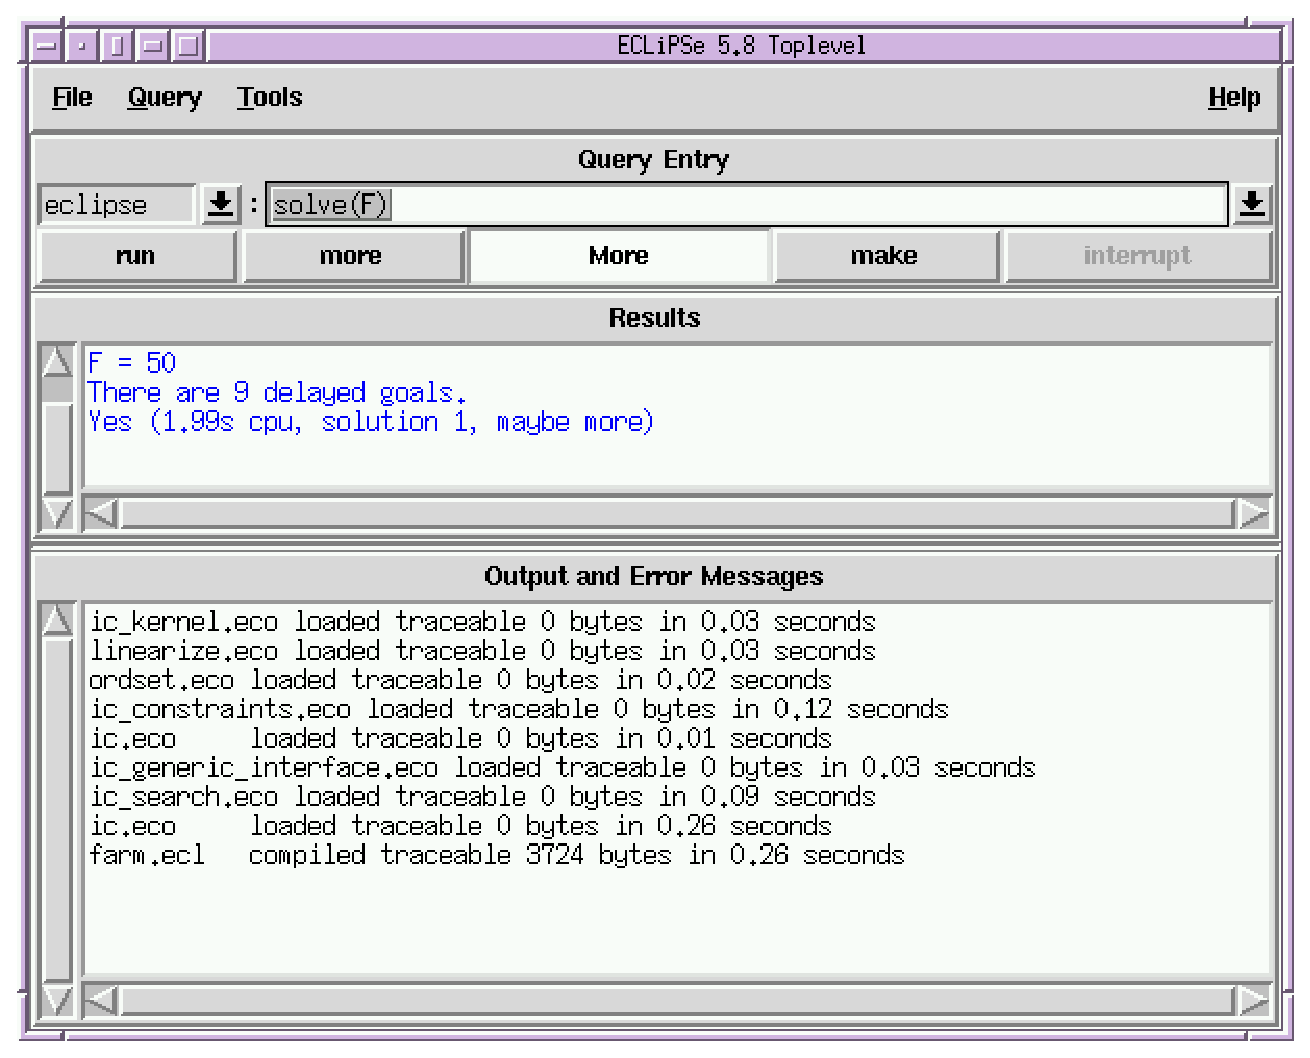
\includegraphics{tktop.eps}}
\end{center}
\caption{{\tkeclipse} top-level}
\label{tktop}
\end{figure}

Note that help on {\tkeclipse} and its component tools is available from the
\menu{Help} menu in the top-level window.
If you need more information than can be found in this manual, try looking
in the \menu{Help} menu.

%------------------------------------------------------------------------
\section{How do I write an {\eclipse} program?}
%------------------------------------------------------------------------
You must use an editor to write your programs. {\eclipse} does not come
with an editor, but any editor that can save plain text files can be used.
Save your program as a plain text file, and you can then compile the
program into {\eclipse} and run it.

With {\tkeclipse}, you can specify the editor you want to use, and this
editor will be started by {\tkeclipse}, e.g., when you select a file in
the `Edit' option under the File menu. The default values are the value of
the VISUAL environment variable  under Unix, or Wordpad under Windows.
This can be changed with the Preference Editor under the Tools menu.

%------------------------------------------------------------------------
\subsection{Compiling a program}

From the \menu{File} menu, select the \menuopt{Compile ...} option.
This will bring up a file selection dialog.
Select the file you wish to compile, and click on the \button{Open} button.
This will compile the file and any others it depends on.
Messages indicating which files have been compiled and describing any errors
encountered will be displayed in the bottom portion of the {\tkeclipse}
window (\guitext{Output and Error Messages}).

If a file has been modified since it was compiled,
it may be recompiled by clicking on the \guitext{make} button.
This recompiles any files which have become out-of-date.

For more information on program compilation and the compiler, please see
chapter \ref{chapcompiler}.

%------------------------------------------------------------------------
\subsection{Executing a query}

To execute a query, first enter it into the \guitext{Query Entry}
text field.
You will also have to specify which module the query should be run from, by
selecting the appropriate entry from the drop-down list to the left of the
\guitext{Query Entry} field.
Normally, the default selection of \guitext{eclipse} will be fine; this will
allow access to all {\eclipse} built-ins and all predicates that have not
explicitly been compiled into a different module.
Selecting another module for the query is only needed if you wish to call a
predicate which is not visible from the \notation{eclipse} module, in which
case you must select that module.
(For more information about the module system, please see chapter
\ref{chapmodules}.)

To actually execute the query, either hit the \keyboard{Enter} key while
editing the query, or click on the \guitext{run} button.
{\tkeclipse} maintains a history of commands entered during the session, and
these may be recalled either by using the drop-down list to the right of the
\guitext{Query Entry} field, or by using the up and down arrow keys while
editing the \guitext{Query Entry} field.

If {\eclipse} cannot find a solution to the query, it will print \notation{No}
in the \guitext{Results} section of the {\tkeclipse} window.
If it finds a solution and knows there are no more, it will print it in the
\guitext{Results} section, and then print \notation{Yes}.
If it finds a solution and there may be more, it will print the solution
found as before, print \notation{More}, and enable the \guitext{more} button.
Clicking on the \guitext{more} button tells {\eclipse} to try to find
another solution.
In all cases it also prints the total time taken to execute the query.

Note that a query can be interrupted during execution by clicking on the
\guitext{interrupt} button.

%------------------------------------------------------------------------
\subsection{Editing a file}
\label{secedit}

If you wish to edit a file (e.g., a program source file), then you may do so
by selecting the \guitext{Edit ...} option from the \guitext{File} menu.
This will bring up a file selection dialog.
Select the file you wish to edit, and click on the \guitext{Open} button.

When you have finished editing the file, save it.
After you've saved it, if you wish to update the version compiled into
{\eclipse} (assuming it had been compiled previously), simply click on the
\guitext{make} button.

You can change which program is used to edit your file by using the
{\tkeclipse} Preference Editor, available from the \guitext{Tools} menu.

%------------------------------------------------------------------------
\subsection{Debugging a program}
\label{secdebug}

To help diagnose problems in {\eclipse} programs, {\tkeclipse} provides the
tracer.
This can be invoked by selecting the \guitext{Tracer} option from the
\guitext{Tools} menu.
The next time a goal is executed, the tracer window will become active,
allowing you to step through the program's execution and examine the
program's state as it executes.

The tracer displays the current call stack and a trace log.
By using the left mouse button in the \guitext{Call Stack} region of the
tracer window, you can bring up a menu of additional operations you can
perform on that goal, such as inspecting it, or setting a spy point on the
predicate in question.
Selecting \guitext{Configure filter ...} from the \guitext{Options} menu
of the tracer will launch the conditional filter.
This filter allows you to
specify conditions on which the tracer should stop at a debug port. This
can be very useful for skipping over unwanted debug ports.

For more information on using the tracer, please see the online help,
available by selecting \guitext{Tracer Help} from the \guitext{Help} menu.

Other {\tkeclipse} tools which are useful while using the tracer are:

\begin{itemize}

\item the predicate browser (available by selecting the \guitext{Predicate
Browser} option from the \guitext{Tools} menu), which is useful for setting
or removing spy points on predicates, or for setting the
\notation{start_tracing}
flag which activates the tracer when a particular predicate is called for
the first time; and

\item the term inspector (available by double left clicking on a term from
the stack window, or by selecting the \guitext{Inspector}
option from the \guitext{Tools} menu), which is useful for examining and
browse the arguments of a term in detail.

\item the delayed goals browser (available by selecting the \guitext{Delayed
Goals} option from the \guitext{Tools} menu), which allows you to inspect
the current list of delayed goals.

\item the display matrix (available either from calls in user's code, or by
interactively selecting terms to be observed from the inspector, tracer or
delay goals tools), which allows you to monitor any changes to a term and
its arguments.

\end{itemize}

More information about debugging in {\eclipse} may be found in chapter
\ref{chapdebug}.

%------------------------------------------------------------------------
\subsection{Getting help}

More detailed help than is provided here can be obtained online.
Simply select the entry from the \guitext{Help} menu on {\tkeclipse}'s
top-level window which corresponds to the topic or tool you are interested
in.

%------------------------------------------------------------------------
\subsection{Other tools}

{\tkeclipse} comes with a number of useful tools.
Some have been mentioned above, but here is a more complete list.
Note that we only provide brief descriptions here; for more details, please
see the online help for the tool in question.

\subsubsection{Compile scratch-pad}

This tool allows you to enter small amounts of program code and have it
compiled.
This is useful for quick experimentation, but not for larger examples or
programs you wish to keep, since the source code is lost when the session is
exited.

\subsubsection{Source File Manager}

This tool allows you to keep track of and manage which source files have
been compiled in the current {\eclipse} session.
You can select files to edit them, or compile them individually, as well as
adding new files.

\subsubsection{Predicate Browser}

This tool allows you to browse through the modules and predicates which have
been compiled in the current session.
It also lets you alter some properties of compiled predicates.

\subsubsection{Source Viewer}

This tool attempts to display the source code for predicates selected in
other tools.

\subsubsection{Delayed Goals}

This tool displays the current delayed goals, as well as allowing a spy
point to be placed on the predicate and the source code viewed.

\subsubsection{Tracer}

As discussed in section \ref{secdebug}, the tracer is useful for debugging
programs.
See also chapter \ref{chapdebug}.

\subsubsection{Inspector}

This tool provides a graphical browser for inspecting terms.
Goals and data terms are displayed as a tree structure.
Sub-trees can be collapsed and expanded by double-clicking.
A navigation panel can be launched which provides arrow buttons as an
alternative way to navigate the tree.

Note that while the inspector window is open, interaction with other
{\tkeclipse} windows is disallowed.
This prevents the term from changing while being inspected.
To continue {\tkeclipse}, the inspector window must be closed.

\subsubsection{Global Settings}

This tool allows the setting of some global flags governing the way
{\eclipse} behaves.
See also the documentation for the
\bipref{set_flag/2}{../bips/kernel/env/set_flag-2.html} and
\bipref{get_flag/2}{../bips/kernel/env/get_flag-2.html} predicates.

\subsubsection{Statistics}

This tool displays some statistics about memory and CPU usage of the
{\eclipse} system, updated at regular intervals.
See also the documentation for the
\bipref{statistics/0}{../bips/kernel/env/statistics-0.html} and
\bipref{statistics/2}{../bips/kernel/env/statistics-2.html} predicates.

\subsubsection{Simple Query}

This tool allows the user to send a simple query to {\eclipse} even while
{\eclipse} is running some program and the Toplevel Query Entry window
is unavailable.
Note that the reply is shown in EXDR format (see the {\eclipse} Embedding
and Interfacing Manual).

\subsubsection{Library Help}

This tool allows you to browse the online help for the {\eclipse} libraries.
On the left is a tree display of the libraries available and the predicates
they provide.
\begin{itemize}
\item Double clicking on a node in this tree either expands it or collapses it
again.
\item Clicking on an entry displays help for that entry to the right.
\item Double clicking on a word in the right-hand pane searches for help
entries containing that string.
\end{itemize}
You can also enter a search string or a predicate specification manually
in the text entry box at the top right.
If there is only one match, detailed help for that predicate is displayed.
If there are multiple matches, only very brief help is displayed for each;
to get detailed help, try specifying the module and/or the arity of the
predicate in the text field.

\subsection{Preference Editor}

This tool allows you to edit and set various user preferences. This include
parameters for how {\tkeclipse} will start up, e.g., the amount of memory it
will be able to use, and an initial query to execute; and parameters which
affects the appearance of {\tkeclipse}, such as the fonts {\tkeclipse}
uses.

%------------------------------------------------------------------------
\section{How do I use \notation{eclipse}?}
%------------------------------------------------------------------------

\subsection{Getting started}

To start {\eclipse}, type the command \notation{eclipse} at an
operating system command-line prompt.
This will display something like this:
\begin{quote}
\begin{verbatim}
% eclipse
ECLiPSe Constraint Logic Programming System [kernel]
Kernel and basic libraries copyright Cisco Systems, Inc.
and subject to the Cisco-style Mozilla Public Licence 1.1
(see legal/cmpl.txt or www.eclipse-clp.org/licence)
Source available at www.sourceforge.org/projects/eclipse-clp
GMP library copyright Free Software Foundation, see legal/lgpl.txt
For other libraries see their individual copyright notices
Version X.Y #Z, DAY MONTH DD HH:MM YYYY
[eclipse 1]:
\end{verbatim}
\end{quote}
The list in square brackets on the first line specifies the configuration
of the running system, i.e., the language extensions that are present.
The copyright and version information is followed by the prompt
\notation{[eclipse 1]:}, which tells the user that the top-level loop is waiting
for a user query in the module \notation{eclipse}.
The predicate \predspecidx{help/0} gives
general help and \bipref{help/1}{../bips/kernel/env/help-1.html} gives
help about specific built-in predicates.

%------------------------------------------------------------------------
\subsection{Interacting with the top level loop}

The {\eclipse} prompt \notation{[eclipse 1]:} indicates that {\eclipse}
is at the top level
and the opened module is \notation{eclipse}.
The \aboutidx{top level loop} is a procedure which repetitively
prompts the user for a query, executes it and reports its
result, i.e., either the answer variable bindings or the
failure message.
There is always exactly one module opened in the top level
and its name is printed in the prompt.
From this point it is possible to enter {\eclipse} goals, e.g., to
pose queries, to enter an {\eclipse} program from the keyboard
or to compile a program from a file.
Goals are entered after the prompt and are terminated by fullstop and
newline.

The {\eclipse} system may be exited by typing \notation{CTRL-D} (UNIX) or
\notation{CTRL-Z} + \notation{RETURN} (Windows) at the top level prompt,
\index{Exiting {\eclipse}}
or by calling either the \bipref{halt/0}{../bips/kernel/opsys/halt-0.html}
or the \bipref{exit/1}{../bips/kernel/opsys/exit-1.html} predicates.

%------------------------------------------------------------------------
\subsection{Compiling a program}

The square brackets \notation{[}\pattern{...}\notation{]} or the
\bipref{compile/1}{../bips/kernel/compiler/compile-1.html} predicate are used
to compile {\eclipse} source from a file.
If the goal
\begin{quote}
\begin{verbatim}
compile(myfile).
\end{verbatim}
\end{quote}
or the short-hand notation
\begin{quote}
\begin{verbatim}
[myfile].
\end{verbatim}
\end{quote}
is called, either as a query at the top level or within another goal,
the system looks for the file \notation{myfile} or for a file called
\notation{myfile.pl} or \notation{myfile.ecl} and compiles it.
The short-hand notation may also be used to compile several files in
sequence:
\begin{quote}
\begin{verbatim}
[ file_1, file_2, ..., file_n ]
\end{verbatim}
\end{quote}
The \bipref{compile/2}{../bips/kernel/compiler/compile-2.html} predicate may be
used to compile a file or list of
files into a module specified in the second argument.

If a file has been modified since it was compiled, it may be recompiled by
invoking the \bipref{make/0}{../bips/kernel/env/make-0.html} predicate.
This recompiles any files which have become out-of-date.

For more information on program compilation and the compiler, please see
chapter \ref{chapcompiler}.

%------------------------------------------------------------------------
\subsection{Entering a program from the terminal}

Programs can be entered directly from the terminal, as well as being read
from files.
To do this, simply compile the special file \notation{user}.
That is, \notation{[user].} or \notation{compile(user).} at a top level
prompt.
The system then displays the compiler prompt (which is a blank by default)
and waits for a sequence of clauses.
Each of the clauses is terminated by a fullstop.%
\index{fullstop}\index{clause!termination}
(If the fullstop is omitted the system just sits
waiting, because it supposes the clause is not terminated.
If you omit the fullstop by accident simply type it in on the following line,
and then proceed to type in the program clauses, each followed by a fullstop and
carriage return.)
To return to the top level prompt,
type CTRL-D (UNIX), CTRL-Z + RETURN (Windows) or enter the atom
\notation{end_of_file} followed by fullstop and RETURN.

For example:
\begin{quote}
\begin{verbatim}
[eclipse 1]: [user].
source_processor.eco loaded in 0.01 seconds
...
ecl_compiler.eco loaded in 0.23 seconds
 father(abraham, isaac).
 father(isaac, jacob).
 father(jacob, joseph).
 ancestor(X, Y) :- father(X, Y).
 ancestor(X, Y) :- ancestor(X, Z), ancestor(Z, Y).
 ^D
 tty        compiled 420 bytes in 0.01 seconds

Yes (0.24s cpu)
[eclipse 2]:
\end{verbatim}
\end{quote}
The two predicates \predspec{father/2} and \predspec{ancestor/2} are now
compiled
and can be used.

%------------------------------------------------------------------------
\subsection{Executing a \Index{query}}

Once a set of clauses has been compiled,
it may be queried in the usual Prolog manner.
If there are uninstantiated \Index{variables} in the query,
the system will attempt to find an instantiation of them which will
satisfy the query, and if successful it will
display one such instantiation.
If potentially there is another solution, the top level
will then wait for a further instruction: either a \notation{<CR>}
(``newline'' or ``return'') or a semi-colon (\notation{;}).
A return will end the query successfully.
A semi-colon will initiate \Index{backtracking}
in an attempt to find another solution to the query.
Note that it is not necessary to type a new line after the semicolon
--- one keystroke is enough.
When the top level loop can detect
that there are no further solutions, it does not wait for the semicolon
or newline, but it displays directly the next prompt.
For example in a query on
a family database:
\begin{quote}
\begin{verbatim}
[eclipse 3]: father(X, Y).

X = abraham
Y = isaac
Yes (0.00s cpu, solution 1, maybe more) ? ;            (user types ';')

X = isaac
Y = jacob
Yes (0.00s cpu, solution 2)
[eclipse 4]:
\end{verbatim}
\end{quote}

Queries may be extended over more than one line. When this is done the prompt
changes to a tabulation character, i.e., the input is indented to
indicate that the query is not yet completed.
The fullstop marks the end of the input.

%------------------------------------------------------------------------
\subsection{Interrupting the execution\index{interrupt}}

If a program is executing, it may be interrupted by
typing \notation{CTRL-C} (interrupt in the UNIX environment).
This will invoke the corresponding interrupt handler
(see section \ref{sectinterrupts}).
By default, the system prints a menu offering some alternatives:
\begin{quote}
\begin{verbatim}
^C
interruption: type a, b, c, e, or h for help : ? h       (user types 'h')
help
	a : abort
	b : break level
	c : continue
	e : exit
	h : help


interruption: type a, b, c, e, or h for help : ?
\end{verbatim}
\end{quote}
The \notation{a} option returns to the toplevel, \notation{b} starts a nested
toplevel,
\notation{c} continues the interrupted execution, and \notation{e} is an
emergency
exit
of the whole {\eclipse} session. If the debugger is running, an additional
option \notation{d} is displayed: it switches the debugger to creep mode.

The execution of {\eclipse} may be suspended by typing \notation{CTRL-Z}
(suspend) or by calling \bipref{pause/0}{../bips/kernel/opsys/pause-0.html}.
This will suspend the {\eclipse} process and return the UNIX prompt.
Entering the shell command \notation{fg} will return to {\eclipse}.
Note that this feature may not be available on all systems.

%------------------------------------------------------------------------
\subsection{Debugging a program}

Please see the chapters on debugging in the tutorial and user manuals for
more details. The tutorial chapter covers the {\tkeclipse} debugging in a
tutorial style tour, and the user manual chapter covers
 debugging in
general and the command-line debugger in particular.

%------------------------------------------------------------------------
\subsection{The \Index{history} mechanism}
The {\eclipse} toplevel loop provides a simple history mechanism which allows
the examination and repetition of previous queries.
The history list is printed with the command \notation{h}.
A previous query is invoked by typing either its absolute number or its
relative negative offset from the current query number (i.e., --1 will
execute the previous query).
The current query number is displayed in the toplevel prompt.

The history is initialized from the file \notationidx{.eclipse_history}
in the current directory or in the home directory.
This file contains the history goals, each ended by a fullstop.
The current history can be written using the predicate
\bipref{write_history/0}{../bips/lib/toplevel/write_history-0.html} from the
\notation{util} library.

%------------------------------------------------------------------------
\subsection{Getting \Index{help}}
Detailed documentation about all the predicates in the {\eclipse} libraries
can be obtained online through the help facility.
It has two modes of operation.
First, when a fragment of a built-in name is specified, a list of short
descriptions of all built-ins whose name contains the specified string
is printed.
For example,
\begin{quote}
\begin{verbatim}
:- help(write).
\end{verbatim}
\end{quote}
will print one-line descriptions about \predspec{write/1},
\predspec{writeclause/2}, etc.
When a unique specification is given, the full description of the
specified built-in is displayed, e.g., in
\begin{quote}
\begin{verbatim}
:- help(write/1).
\end{verbatim}
\end{quote}

%------------------------------------------------------------------------
\section{How do I make things happen at compile time?}
%------------------------------------------------------------------------

A file being compiled may contain queries.\index{query}
These are goals preceded by the symbol ``:-''.
As soon as a query is encountered in the compilation of a file,
the {\eclipse} system will try to satisfy it.
Thus by inserting goals in this fashion, things can be made to happen at
compile time.

In particular, a file can contain a directive to the system
to compile another file, and so large programs can be split between files,
while still only requiring a single simple command to compile them.%
\index{compilation!nesting compile commands}
When this happens, {\eclipse} interprets the pathnames of the nested
compiled files relative to the directory of the parent compiled file;
if, for example, the user calls
\begin{quote}
\begin{verbatim}
[eclipse 1]: compile('src/pl/prog').
\end{verbatim}
\end{quote}
and the file src/pl/prog.pl contains a query
\begin{quote}
\begin{verbatim}
:- [part1, part2].
\end{verbatim}
\end{quote}
then the system searches for the files \notation{part1.pl} and
\notation{part2.pl}
in the
directory \notation{src/pl} and not in the current directory.
Usually larger {\eclipse} programs have one main file which contains
only commands to compile all the subfiles.
In {\eclipse} it is possible to compile this main file from any directory.
(Note that if your program is large enough to warrant breaking into multiple
files (let alone multiple directories), it is probably worth turning the
constituent components into modules --- see chapter \ref{chapmodules}.)

%------------------------------------------------------------------------
\section{How do I use {\eclipse} \Index{libraries} in my programs?}
%------------------------------------------------------------------------

A number of files containing library predicates are supplied with
the {\eclipse} system.
These predicates provide utility functions for general use.
They are usually installed in an {\eclipse} library directory (or
directories).
These predicates are either loaded automatically by {\eclipse} or may be
loaded ``by hand''.

During the execution of an {\eclipse} program, the system may dynamically
load files containing library predicates. When this happens, the user is
informed by a compilation or loading message.
It is possible to explicitly force this loading to occur by use
of the \bipref{lib/1}{../bips/kernel/compiler/lib-1.html} or
\bipref{use_module/1}{../bips/kernel/modules/use_module-1.html} predicates.
e.g., to load the library
called \notation{lists}, use one of the following goals:
\begin{quote}
\begin{verbatim}
lib(lists)
use_module(library(lists))
\end{verbatim} 
\end{quote}
This will load the library file unless it has been already loaded.
In particular, a program can ensure that a given library is loaded when it
is compiled, by including an appropriate directive in the source, e.g.,
\notation{:- lib(lists).}

Library files are found by searching the
\Index{library path}\index{library search path}
and by appending a suffix to the library name.
The search path used when loading libraries is
specified by the global flag \notation{library_path} using the
\bipref{get_flag/2}{../bips/kernel/env/get_flag-2.html} and
\bipref{set_flag/2}{../bips/kernel/env/set_flag-2.html} predicates.
This flag contains a list of strings containing the pathnames of the
directories to be searched when loading a library file.
User libraries may be be added to the system simply by copying the
desired file into the {\eclipse} library directory.
Alternatively the \notation{library_path} flag may be updated to point
at a number of user specific directories. The following example illustrates
how a directive may be added to a file to add a user-defined library in front
of any existing system libraries.
\begin{quote}
\begin{verbatim}
?- get_flag(library_path,Path),
   set_flag(library_path, ["/home/myuser/mylibs" | Path]).
\end{verbatim}
\end{quote}
The UNIX environment variable \notationidx{ECLIPSELIBRARYPATH} may also be used
to
specify the initial setting of the library path.
The syntax is similar to the syntax of the UNIX PATH variable, i.e.,
a list of directory names separated by colons.
The directories will be prepended to the standard library path in the
given order.

%------------------------------------------------------------------------
\section{How do I make my programs run faster?}
%------------------------------------------------------------------------

By default, {\eclipse} compiles programs as \about{traceable}, which
means that they can be traced using the built-in debugger.
To obtain maximum efficiency, the directive
\bipref{nodbgcomp/0}{../bips/kernel/obsolete/nodbgcomp-0.html}
should be used, which will set some flags to produce a more efficient
and shorter code:
\begin{quote}
\begin{verbatim}
[eclipse 2]: nodbgcomp.

yes.
[eclipse 3]: [user].
 father(abraham, isaac).
 father(isaac, jacob).
 father(jacob, joseph).
 ancestor(X, Y) :- father(X, Y).
 ancestor(X, Y) :- ancestor(X, Z), ancestor(Z, Y).
  user       compiled optimized 396 bytes in 0.02 seconds

yes.
[eclipse 4]:
\end{verbatim}
\end{quote}

Section \ref{secefficientcode} contains more detailed discussion on other
techniques which can be used to optimise your programs.


%------------------------------------------------------------------------
\section{Other tips}
%------------------------------------------------------------------------

%------------------------------------------------------------------------
\subsection{Initialization at start-up}

If you wish to have {\eclipse} do or execute things at startup time, you
can achieve this in {\tkeclipse} by setting the initial query call in the
Preference editor; and in the command-line \notation{eclipse} by putting via a
\notation{.eclipserc} file.

For \notation{eclipse},
before displaying the initial prompt, the system checks whether there is a file
called \notationidx{.eclipserc}\index{initialization file}\label{eclipserc}
in the current directory and if not, in the user's home
directory.  If such a file is found, {\eclipse} compiles it first.
Thus it is possible to put various initialization commands into
this file.
{\eclipse} has many possibilities to change its default behaviour and
setting up a \notation{.eclipserc} file is a convenient way to achieve this.
A different name for the initialization file can be specified
in the environment variable \notationidx{ECLIPSEINIT}.
If \notation{ECLIPSEINIT} is set to an empty string, no initialization is done.
If the system is started with a -e option, then the \notation{.eclipserc} file
is ignored.

For {\tkeclipse}, the system will make the initial query call as set in the
Preference Editor before giving control to the user. This call can be set
to compile an initialization file. This can be the \notation{.eclipserc} file,
or some other file if the user wants to initialize the system differently in
{\tkeclipse}.

%------------------------------------------------------------------------
\subsection{Recommended file names}

It is recommended programming practice to give the Prolog source programs
the suffix \notation{.pl}, or \notation{.ecl} if it contains {\eclipse} specific
code.
It is not enforced by the system, but it simplifies managing the source
programs.
The \bipref{compile/1}{../bips/kernel/compiler/compile-1.html} predicate
automatically adds the suffix to the
file name, so that it does not have to be specified;
if the literal file name can not be found, the system tries appending
each of the valid suffixes in turn and tries to find the resulting file name.
The system's list of valid Prolog suffixes is in the global flag
\notationidx{prolog_suffix} and can be examined and modified
using \bipref{get_flag/2}{../bips/kernel/env/get_flag-2.html} and
\bipref{set_flag/2}{../bips/kernel/env/set_flag-2.html}.
For example, to add the new suffix \notation{.pro} use:
\begin{quote}
\begin{verbatim}
get_flag(prolog_suffix, Old), set_flag(prolog_suffix, [".pro"|Old]).
\end{verbatim}
\end{quote}

%HEVEA\cutend

% BEGIN LICENSE BLOCK
% Version: CMPL 1.1
%
% The contents of this file are subject to the Cisco-style Mozilla Public
% License Version 1.1 (the "License"); you may not use this file except
% in compliance with the License.  You may obtain a copy of the License
% at www.eclipse-clp.org/license.
%
% Software distributed under the License is distributed on an "AS IS"
% basis, WITHOUT WARRANTY OF ANY KIND, either express or implied.  See
% the License for the specific language governing rights and limitations
% under the License.
%
% The Original Code is  The ECLiPSe Constraint Logic Programming System.
% The Initial Developer of the Original Code is  Cisco Systems, Inc.
% Portions created by the Initial Developer are
% Copyright (C) 2006 Cisco Systems, Inc.  All Rights Reserved.
%
% Contributor(s):
%
% END LICENSE BLOCK
\chapter{The {\tkeclipse} Development Tools}
\label{chaptkeclipse}
%HEVEA\cutdef[1]{section}

{\tkeclipse} is a graphical user interface to {\eclipse}. It is an
alternative to the traditional textual line-based user interface, providing
multiple windows, menus and buttons to assist the user in interacting with
{\eclipse}. It consists of two major components:

\begin{itemize}
\item A graphical top-level.
\item A suite of development tools for aiding the development of {\eclipse}
code.
\end{itemize}

{\tkeclipse} is implemented in the Tcl/Tk scripting language/graphical toolkit
\cite{Tcl94}, using the new {\eclipse} Tcl/Tk interface
\cite{interfaceManual}. The development tools are designed to be
independent of the top-level, so the users can develop their own
applications with a graphical front end written in Tcl/Tk, replacing the
{\tkeclipse} top-level, but still using the development tools.

Chapter \ref{chapusing} gave an introduction to using {\tkeclipse} from a
user's point of view.
This chapter focuses on how to use the tools from a programmer's point of
view (i.e., how to include them in a program).
In particular it discusses in detail the \toolname{display matrix} tool, which
can be invoked in user's {\eclipse} code; and also how to use the
development tools in the user's own applications.

\section{Display Matrix}
\label{displaymat}

This tool provides a method to display the values of terms in a matrix
form. It is particularly useful because it can display the attributes of an
attributed variable.\footnote{%
  The display matrix tool is similar to the variable display of
  \toolname{Grace}.
  The main differences are:
  it can display all attributes, not just the finite domain attribute;
  the attributes can only be observed, not changed;
  and the labelling strategy cannot be changed.}
The predicate which invokes the display matrix is considered a no-op
in the tty-based {\eclipse},\footnote{%
  Unless it is attached to the remote
  development tools, in which case the display matrix is invoked.}
and so the same code can be run without
modification from either \texttt{eclipse} or \texttt{tkeclipse}, though
the matrix display is only presented to the user in the latter.

To invoke this tool use either
\bipref{make_display_matrix/2}%
{../bips/kernel/debug/make_display_matrix-2.html}
or
\bipref{make_display_matrix/5}%
{../bips/kernel/debug/make_display_matrix-5.html}.
Adding a call to one of these predicates should be the only change you need
to make to your code.
For example, in the following fragment of a N-queens program, only one
extra line has been added to invoke a display matrix:
\vfill      %<<<<<<<<<<<<<<
\pagebreak  %<<<<<<<<<<<<<<
\begin{quote}
\begin{verbatim}
   queens(N, List) :-
       length(List, N),
       List :: 1..N,
       make_display_matrix(List/0, queens),
       % sets up a matrix with all variables in 1 row. This is the only
       % extra goal that has to be added to enable monitoring
       alldistinct(List),
       constrain_queens(List),
       labeling(List).
\end{verbatim}
\end{quote}

\begin{figure}[bt]
\begin{center}
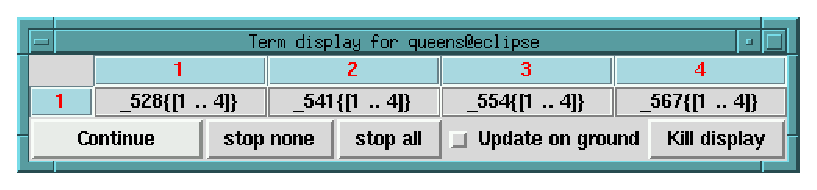
\includegraphics{dismat.eps}
\end{center}
\caption{Display Matrix Tool for 4-Queens (Initial)}
\label{dismat}
\end{figure}

\begin{figure}[bt]
\begin{center}
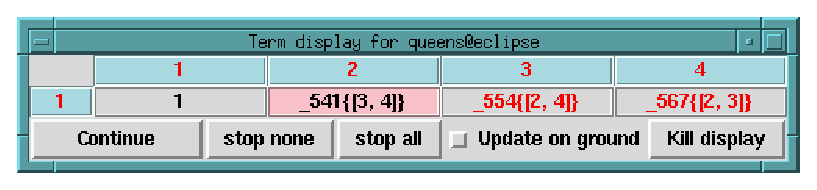
\includegraphics{dismat2.eps}
\end{center}
\caption{Display Matrix Tool for 4-Queens (During execution)}
\label{dismat2}
\end{figure}

Figures~\ref{dismat} and \ref{dismat2} show the tool
invoked with the example N-Queens programs for 4 Queens, at the start
initially and during the execution of the program. The name of the display
window is specified by the second argument of
\bipref{make_display_matrix/2}%
{../bips/kernel/debug/make_display_matrix-2.html},
along with the module it is in. The values of the terms are shown in the
matrix, which can be one dimensional (as in this case), or two
dimensional. Spy points can be set on each individual cell of the matrix
so that execution will stop when the cell is updated. The matrix can be
killed using the `Kill display' button. Left-clicking on a cell will bring
up a menu which shows the current and previous value of the term in the
cell (the current value is shown because the space available in the cell
may be too small to fully display the term), and allows the user to inspect
the term using the inspector.

Note that the display matrix can be used independently of, or in conjunction
with, the tracer. Multiple display matrices can be created to view
different terms.

The following predicates are available in conjunction with the display
matrix:

\medskip
\begin{quote}
\preddef{make_display_matrix(+\pattern{Terms},~+\pattern{Name})}%
\indextt{make_display_matrix/2}\\
\preddef{make_display_matrix(%
+\pattern{Terms},~+\pattern{Prio},~+\pattern{Type},%
~+\pattern{CondList},~+\pattern{Name})}%
\indextt{make_display_matrix/5}
\end{quote}

These
predicates create a display matrix of terms that can be monitored under
{\tkeclipse}. The two argument form is a simplification of the five argument
form, with defaults settings for the extra arguments.
\about{Terms} is a list or
array of terms to be displayed.
A list \about{List} can be specified in the form \pattern{List/N},
where \about{N} is the number of elements per row of the matrix.
If \about{N} is 0, then
the list will be displayed in one row (it could also be omitted in this
case). The extra arguments are used to control how the display is updated.

   The terms are monitored by placing a demon suspension on the variables
   in each term. When a demon wakes, the new value of the term it is
   associated with is sent to the display matrix (and possibly updated,
   depending on the interactive settings on the matrix). When the new
   value is retracted during backtracking,
   the old value is sent to the display matrix.
   The other arguments in this predicate are used to control when the
   demon wakes, and what sort of information is monitored. \about{Prio} is the
   priority that the demon should be suspended at, \about{Type} is designed to
   specify the attributes that are being monitored (currently all
   attributes are monitored, and
   \about{Type} is a dummy argument), \about{CondList} is
   the suspension list that the demon should be added to. Depending on
   these arguments, the level of monitoring can be controlled. Note that
   it is possible for the display matrix to show values that are out of
   date because the change was not monitored.

   The display matrix will be removed on backtracking. However, it will
   not be removed if \predspec{make_display_matrix} has been
   cut: \predspec{kill_display_matrix/1} can be used to explicitly remove
   the
   matrix in this case.

\medskip
\begin{quote}
\preddef{kill_display_matrix(+\pattern{Name})}%
\indextt{kill_display_matrix/1}
\end{quote}

This predicate destroys an existing
   display matrix. \about{Name} is an atomic term which identifies the matrix.

   Destroys an existing display matrix. The display matrix is removed
   from being displayed.


\subsection{Invoking display matrix tool interactively}

Display matrices can be created interactively when a program is
executing, if the program is being debugged with the tracer tool. The user
can select terms that are to be observed by a display matrix while at a
debug port. This can be done from the inspector, the tracer, and the delay
goal tools. See the online help files (available from the help menu of
{\tkeclipse}) for more details.

\section{Using the development tools in applications}

The user can develop their own {\eclipse} applications using the
development tools independently of the {\tkeclipse} toplevel. There are two
ways to do this, depending on if the user is also using the embedding Tcl/Tk
interface (see the Embedding and Interfacing Manual) to provide a graphical
front end:

\begin{itemize}
\item The user is using the embedding Tcl/Tk interface, and is thus
developing a graphical front end in Tk. In this case the user can use the
 development tools via the embedding interface. This is described in
 section~\ref{embedtools}.
\item The user is not using the embedding Tcl/Tk interface. In this case
 the user can use the development tools remotely, by using the remote_tools
 library. This is described in section~\ref{useremotetools}.
\end{itemize}

\subsection{Using the Development tools in the Tcl/Tk Embedding Interface}
\label{embedtools}

 The development tool suite was
designed to be independent of the {\tkeclipse} top-level so that they can be
used in a user's application. In effect, the user can replace the
{\tkeclipse}
top-level with their own alternative top-level. Two simple examples in
which this is done are provided in the \verb'lib_tcl' library as
\verb'example.tcl' and \verb'example1.tcl'. In addition, \verb'tkeclipse'
itself, in the file \verb'tkeclipse.pl', can be seen as a more complex
example usage of the interface.

In order to use the Tcl/Tk interface, the system must be initialized as
described in the Embedding manual. In addition, the user's Tcl code should
probably also be provided as a package using Tcl's package facility, in
order to allow the program to run in a different directory. See the
Embedding manual and the example programs for more details on the
initialization needed.

The user should most likely provide a connection for the output stream
of {\eclipse} so that output from {\eclipse} will go somewhere in the GUI. In
addition, especially during the development, it is also useful to connect
the error stream to some window so that errors (such as {\eclipse}
compilation errors) are seen by the user. This can be done using the
\verb'ec_queue_connect' Tcl command described in the embedding manual.

Output from {\eclipse} need not be sent to a Tk window directly. The Tcl/Tk
code which receives the output can operate on it before displaying it. It
is intended that all such graphical operations should be performed on the
Tcl side, rather than having some primitives provided on the {\eclipse} side.


The user can also provide balloon-help to his/her own application. The
balloon help package is part of the Megawidget developed by Jeffrey Hobbs
and used in {\tkeclipse}. In order to define a balloon help for a particular
widget, the following Tcl code is needed:

\begin{quote}
\begin{verbatim}
balloonhelp <path> <text>
\end{verbatim}
\end{quote}

\noindent
where \verb'<path>' is the pathname of the widget, and \verb'<text>' is the
text that the user wants to display in the balloon.


\subsection{Using the Remote Development Tools}
\label{useremotetools}

The user can also use the development tools via the remote_tools
library. In this case, the development tools are run as a separate program
from the {\eclipse} session, and are attached to it via the Tcl/Tk remote
interface (see the Embedding and Interfacing Manual). This allows any
{\eclipse} session to use the development tools,
as long as there is the capability for graphical display.

The main purpose for the remote_tools library is to allow the user to
use the development tools in situations where (s)he cannot use the Tcl/Tk
embedding interface, e.g., if {\eclipse} is already embedded into another
programming language, or if the user has to use the tty interface for
{\eclipse}.

\begin{figure}[bt]
\begin{center}
\centering{
\mbox{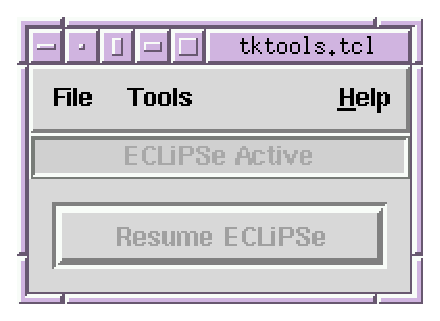
\includegraphics{remotetools.eps}}
\mbox{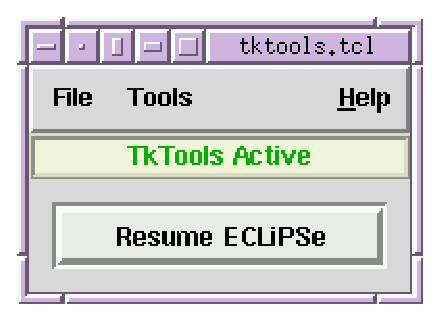
\includegraphics{remotetools2.eps}}
}
\end{center}
\caption{Remote Development Tools Toplevel (left: {\eclipse} active; right:
remote tools active)}
\label{remotetools}
\end{figure}

Once attached to an {\eclipse} session, the remote development tools have
their own window as shown in Figure~\ref{remotetools}. The Tools menu is the
same as in {\tkeclipse}, providing access to the same suite of development
tools. The main body of the window consists of one button and a status
indicator. The indicator shows whether the tools can be used or not (the
tools cannot be used when the {\eclipse} is active), and the button
is used to pass control explicitly to {\eclipse}.

The {\eclipse} session and the development tools are two separate processes
(and in fact they can be running on different machines) that are connected
to each other via the remote Tcl/Tk interface. The interactions of the two
processes are synchronised in that there is a thread-like flow of control
between them: only one process can be `active' at any time. The interaction
is similar to the standard interaction between a debugger and the program
being debugged -- debugging commands can only be issued
while the execution of the program is suspended. In the same way, the user
can only interact with the remote tools window when execution in the
{\eclipse} session is suspended. The toplevel window of the remote tools
has an indicator showing which side has control (see Figure~\ref{remotetools}).
To allow {\eclipse} to resume execution, control is transferred back from
the remote tools to {\eclipse}. This can either be
done automatically from the tools (e.g., when one of the debug buttons is
pressed in the tracer tool), or control can be transferred explicitly back
to {\eclipse} via the ``Resume ECLiPSe'' button on the remote tools window.


\subsubsection{Starting Remote Tools}

To use the remote tools, the user must first load the right library
with \verb'lib(remote_tools)'. After loading the library, the user can
start the remote tools by
starting the development tools as a separate program and then manually
attaching the program to the {\eclipse} session. This allows the development
tools to be run on a different machine from the {\eclipse} session. In this
case, the user initiates the attachment in {\eclipse} with
\bipref{attach_tools/0}{../bips/lib/remote_tools/attach_tools-0.html}:

\begin{quote}
\begin{verbatim}
[eclipse 2]: attach_tools.
Socket created at address holborn.icparc.ic.ac.uk/22849
\end{verbatim}
\end{quote}

{\eclipse} prints the host and port address it expects the remote tools to
attach to, and execution is now suspended waiting for the remote tools to
attach. This is done by running the \toolname{tktools} program, which is located
with the other {\eclipse} executables. As stated, this program can be run
on a different machine from the {\eclipse} session, as long as the two are
connected via a network such as the internet. A connection window is then
displayed as shown:
\vfill %<<<<<<<<<<<

\begin{center}
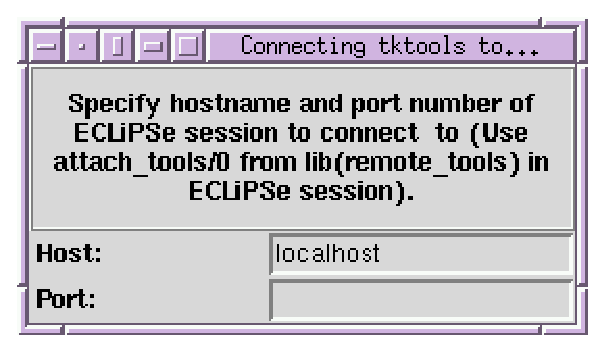
\includegraphics{remotecon.eps}
\end{center}

The same `host' and `port' fields as printed by the {\eclipse} session should
be entered. The default `host' field is `localhost'. This will work if the
remote tools are ran on the same machine as the {\eclipse}
session. Otherwise the full name of the `host' as given by
\predspec{attach_tools/0} must be entered:

\begin{center}
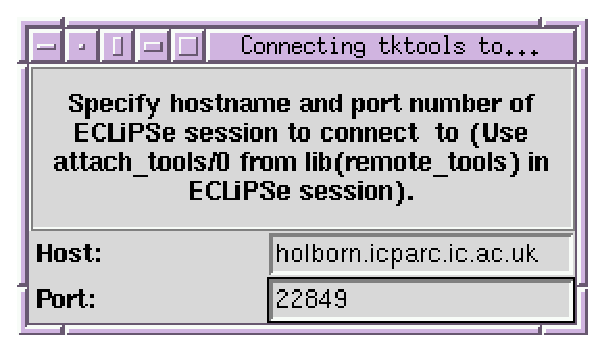
\includegraphics{remotecon2.eps}
\end{center}

Typing return in the `port' field will start the attachment, and with
success, the remote tools window (see Figure~\ref{remotetools}) will be
displayed. The \predspec{attach_tools/0} predicate will also return.

The user is not able to immediately interact directly with the remote
tools, as the {\eclipse} session is initially given control. The user can
use the {\eclipse} session normally, with the additional availability of
the development tools. For example, the display matrix predicates can be
used as in {\tkeclipse}. Also, the tracer tool replaces the previous
tracing facilities of the {\eclipse} session (this would typically be the
command-line debugger).

The tools can be triggered by events in the {\eclipse} session as described
above. In order to use the tools in a more interactive way, control should
be handed over to the remote tools. This can be done by calling the
\bipref{tools/0}{../bips/lib/remote_tools/tools-0.html} predicate.
When the remote tools have control, the user can
now interactively select development tools from the Tools menu.

The remote_tools library provides several predicates to facilitate the use
of the remote development tools:

\begin{quote}
\begin{description}
\item[tools\indextt{tools/0}] Explicitly hands over control to the remote
development
tools. The tools window can then be used interactively. Execution on the
{\eclipse} session is suspended until the remote tools allows {\eclipse} to
resume, at which point the predicate succeeds. The predicate will abort if
the development tools are disconnected from the {\eclipse} session.

\item[attached(?\pattern{ControlStream})\indextt{attached/1}]
	Checks if the remote development tools have been attached to this
        {\eclipse} session or not. If attached, the predicate succeeds and
        unifies \about{ControlStream} with the stream name of the control
        stream. If not attached, the  predicate fails.

\end{description}
\end{quote}

Once attached, the remote development tools should be connected until the
user quits the session. Although it is possible to disconnect the tools
from the {\eclipse} session (from the File menu in the development tools
window), this is not recommended, as there would not be any debugging
facilities available after the disconnection -- the original tracer would
not be restored.

It is possible to attach the remote development tools to any {\eclipse}
session, including one that is using the embedding Tcl/Tk interface (and
indeed, to {\tkeclipse} itself). However, using the tools via the embedding
interface is usually the better option if available, because the tools are
more tightly coupled to {\eclipse} in this case. This means that the
communications between {\eclipse} and the tools are more efficient (and
hence something like the display matrix would perform more efficiently).


%HEVEA\cutend


% BEGIN LICENSE BLOCK
% Version: CMPL 1.1
%
% The contents of this file are subject to the Cisco-style Mozilla Public
% License Version 1.1 (the "License"); you may not use this file except
% in compliance with the License.  You may obtain a copy of the License
% at www.eclipse-clp.org/license.
%
% Software distributed under the License is distributed on an "AS IS"
% basis, WITHOUT WARRANTY OF ANY KIND, either express or implied.  See
% the License for the specific language governing rights and limitations
% under the License.
%
% The Original Code is  The ECLiPSe Constraint Logic Programming System.
% The Initial Developer of the Original Code is  Cisco Systems, Inc.
% Portions created by the Initial Developer are
% Copyright (C) 2006 Cisco Systems, Inc.  All Rights Reserved.
%
% Contributor(s): Joachim Schimpf, IC-Parc
%
% END LICENSE BLOCK
%
% $Id: umslanguage.tex,v 1.4 2009/12/17 08:22:12 jschimpf Exp $
%
% AUTHOR        Joachim Schimpf, IC-Parc, Imperial College, London
%

%----------------------------------------------------------------------
\chapter{\eclipse-specific Language Features\label{chaplanguage}}
%----------------------------------------------------------------------

%HEVEA\cutdef[1]{section}

{\eclipse} is a logic programming language derived from Prolog.
This chapter describes \eclipse-specific language constructs
that have been introduced to overcome some of the main deficiencies
of Prolog.

%----------------------------------------------------------------------
\section{Structure Notation\label{chapstruct}}
%----------------------------------------------------------------------

\index{structures}
{\eclipse} \Index{abstract structure notation}%
\index{structure notation|see{abstract structure notation}}
provides a way to use structures with
field names. It is intended to make programs more readable and easier
to modify, without compromising efficiency
(it is implemented by parse-time preprocessing).

A structure is declared by specifying a template like this
\indextt{local/1}
\indextt{export/1}
\indextt{struct/1}
\begin{quote}
\begin{verbatim}
:- local struct( book(author, title, year, publisher) ).
\end{verbatim}
\end{quote}
Structures with the functor \about{book/4} can then be written as%
\index{curly braces}%
\indextt{with/2}
\begin{quote}
\begin{verbatim}
book{}
book{title:'tom sawyer'}
book{title:'tom sawyer', year:1886, author:twain}
\end{verbatim}
\end{quote}
which translate to the corresponding forms
\begin{quote}
\begin{verbatim}
book(_, _, _, _)
book(_, 'tom sawyer', _, _)
book(twain, 'tom sawyer', 1886, _)
\end{verbatim}
\end{quote}
This transformation is done by the parser, therefore it can
be used in any context and is as efficient as using the structures
directly.

The argument index of a field in a structure can be obtained
using a term of the form
\indextt{of/2}
\begin{quote}
\begin{verbatim}
FieldName of StructName
\end{verbatim}
\end{quote}
For example, to access (i.e., unify) a single argument of a structure
use \predspec{arg/3} like this:
\begin{quote}
\begin{verbatim}
..., arg(year of book, B, Y), ...
\end{verbatim}
\end{quote}
which is translated into
\begin{quote}
\begin{verbatim}
..., arg(3, B, Y), ...
\end{verbatim}
\end{quote}

If a program is consistently written using the abstract structure notation
(i.e., with \notation{\{...\}} and \notation{of}), then the struct-declaration
can be modified (fields added or rearranged) without having to update the code
anywhere else.


\subsection{Updating Structures}

To construct an updated structure, i.e., a structure which is similar
to an existing structure except that one or more fields have new
values, use the
\bipref{update_struct/4}{../bips/kernel/termmanip/update_struct-4.html}
built-in, which allows you to do that without having to mention all the
other field names in the structure.


\subsection{Arity and Functor of Structures}

The arity of a structure can be symbolically written using \predspec{of/2}
as follows:
\begin{quote}\begin{verbatim}
property(arity) of StructName
\end{verbatim}\end{quote}
For example,
\begin{quote}\begin{verbatim}
?- printf("A book has %d fields%n", [property(arity) of book]).
A book has 4 fields
Yes.
\end{verbatim}
\end{quote}
Similarly, the whole \pattern{StructName/Arity} specification can be written as
\begin{quote}
\begin{verbatim}
property(functor) of StructName
\end{verbatim}
\end{quote}
which is used for the portray-declaration in the example below.


\subsection{Printing Structures}
When structures are printed, they are not translated back into the
abstract structure syntax by default. The reason this is not done is that this
can
be bulky if all fields are printed, and often
it is desirable to hide some of the fields anyway.

A good way to control printing of big structures is to write customized
 portray-transformations for them, for instance
\begin{quote}
\begin{verbatim}
:- local portray(property(functor) of book, tr_book_out/2, []).
tr_book_out(book{author:A,title:T},
        no_macro_expansion(book{author:A,title:T})).
\end{verbatim}
\end{quote}
\indextt{no_macro_expansion/1}
which will cause \predspec{book/4} structures to be printed like
\begin{quote}
\begin{verbatim}
book{author:twain, title:tom sawyer}
\end{verbatim}
\end{quote}
while the other two arguments remain hidden.

\subsection{Inheritance}
\index{inheritance}\index{structures!inheritance}
Structures can be declared to contain other structures,
in which case they inherit the base structure's field names.
Consider the following declarations:
\begin{quote}
\begin{verbatim}
:- local struct(person(name,address,age)).
:- local struct(employee(p:person,salary)).
\end{verbatim}
\end{quote}
The \notation{employee} structure contains a field \notation{p} which is a
\notation{person} structure.
Field names of the \verb+person+ structure can now be used as if
they were field names of the \notation{employee} structure:
\begin{quote}
\begin{verbatim}
[eclipse 1]: Emp = employee{name:john,salary:2000}.
Emp = employee(person(john, _105, _106), 2000)
yes.
\end{verbatim}
\end{quote}
Note that, as long as the abstract structure notation is used,
the \notation{employee} structure can be viewed either as nested or as flat,
depending on what is more convenient in a given situation.
In particular, the embedded structure can still be accessed as a whole:
\begin{quote}
\begin{verbatim}
[eclipse 1]:
        Emp = employee{name:john,age:30,salary:2000,address:here},
        arg(name of employee, Emp, Name),
        arg(age of employee, Emp, Age),
        arg(salary of employee, Emp, Salary),
        arg(address of employee, Emp, Address),
        arg(p of employee, Emp, Person).

Emp = employee(person(john, here, 30), 2000)
Name = john
Age = 30
Salary = 2000
Address = here
Person = person(john, here, 30)
yes.
\end{verbatim}
\end{quote}
The indices of nested structures expand into
lists of integers rather than simple integers,
e.g., \notation{age of employee} expands into \notation{[1,3]}.


\subsection{Visibility}
Structure declaration can be local to a module (when declared as above)
or exported when declared as
\indextt{export/1}
\begin{quote}
\begin{verbatim}
:- export struct(...).
\end{verbatim}
\end{quote}
in the module.


%----------------------------------------------------------------------
\section{Loop/Iterator Constructs}
%----------------------------------------------------------------------
\label{doloops}
\index{loops}
\index{iteration}
Many types of simple iterations are inconvenient to write in the
form of recursive predicates. {\eclipse} therefore provides a logical
iteration construct
\bipref{do/2}{../bips/kernel/control/do-2.html},
which can be understood either by itself
or by its translation to an equivalent recursion.

A simple example is the traversal of a list
\begin{quote}
\begin{verbatim}
main :-
        write_list([1,2,3]).

write_list([]).
write_list([X|Xs]) :-
        writeln(X),
        write_list(Xs).
\end{verbatim}
\end{quote}
which can be written as follows without the need for an auxiliary predicate:
\begin{quote}
\begin{verbatim}
main :-
        ( foreach(X, [1,2,3]) do
            writeln(X)
        ).
\end{verbatim}
\end{quote}
This looks very much like a loop in a procedural language. However,
due to the relational nature of logic programming, the same \predspec{foreach}
construct can be used not only to control iteration over an existing list,
but also to build a new list during an iteration. For example
\begin{quote}
\begin{verbatim}
main :-
        ( foreach(X, [1,2,3]), foreach(Y, Negatives) do
            Y is -X
        ),
        writeln(Negatives).
\end{verbatim}
\end{quote}
will print \notation{[-1, -2, -3]}.

The general form of a do-loop is
\begin{quote}
\preddef{(~\pattern{IterationSpecs}~do~\pattern{Goals}~)}\indextt{do/2}
\end{quote}
and it corresponds to a call to an auxiliary recursive
predicate of the form
\begin{quote}
\begin{verbatim}
    do__n(...).
    do__n(...) :- Goals, do__n(...).
\end{verbatim}
\end{quote}

The \about{IterationSpecs} determine the number of times the loop is executed
(i.e., the termination condition), and the way information is passed
into the loop, from one iteration to the next, and out of the loop.

\about{IterationSpecs} is one (or a comma-separated sequence) of the following:

\begin{quote}
\begin{description}
\item[fromto(\pattern{First},~\pattern{In},~\pattern{Out},~\pattern{Last})]%
\index{fromto@\notation{fromto}---iterator construct}\mbox{}\\
    iterate \about{Goals} starting with \about{In=First} until
    \about{Out=Last}.
    \about{In} and \about{Out} are local variables in \about{Goals}.
    For all but the first iteration, the value of \about{In} is the same as the
    value of \about{Out} in the previous iteration.

\item[foreach(\pattern{X},~\pattern{List})]%
\index{foreach@\notation{foreach}---iterator construct}\mbox{}\\
    iterate \about{Goals} with \about{X} ranging over all elements of
    \about{List}.
    \about{X} is a local variable in \about{Goals}.
    Can also be used for constructing a list.

\item[foreacharg(\pattern{X},~\pattern{Struct})]%
\index{foreacharg@\notation{foreacharg}---iterator construct}\mbox{}\\
    iterate \about{Goals} with \about{X} ranging over all elements of
    \about{Struct}.
    \about{X} is a local variable in \about{Goals}.
    Cannot be used for constructing a term.

\item[foreacharg(\pattern{X},~\pattern{Struct},~\pattern{Idx})]
\index{foreacharg@\notation{foreacharg}---iterator construct}\mbox{}\\
    same as before, but \about{Idx} is set to the argument position of \about{X}
    in \about{Struct}. (In other words, \notation{arg(Idx,~Struct,~X)} is true.)
    \about{Idx} is a local variable in \about{Goals}.

\item[foreachelem(\pattern{X},~\pattern{Array})]%
\index{foreachelem@\notation{foreachelem}---iterator construct}\mbox{}\\
    like \predspec{foreacharg/2}, but iterates over all elements of an array
    of arbitrary dimension.  The order is the natural order, i.e.,
    if\\
    \hbox{\hspace{2em}}\notation{Array~=~[]([](a,~b,~c),~[](d,~e,~f))},\\
    then for successive
    iterations \about{X} is bound in turn to \about{a}, \about{b}, \about{c},
    \about{d}, \about{e} and \about{f}.
    \about{X} is a local variable in \about{Goals}.
    Cannot be used for constructing a term.

\item[foreachelem(\pattern{X},~\pattern{Array},~\pattern{Idx})]%
\index{foreachelem@\notation{foreachelem}---iterator construct}\mbox{}\\
    same as before, but \about{Idx} is set to the index position of \about{X} in
    \about{Array}. (In other words, \notation{subscript(Array,~Idx,~X)} is
    true.)
    \about{Idx} is a local variable in \about{Goals}.

\item[foreachindex(\pattern{Idx},~\pattern{Array})]%
\index{foreachindex@\notation{foreachindex}---iterator construct}\mbox{}\\
    like \predspec{foreachelem/3}, but returns just the index position and not
    the element.

\item[for(\pattern{I},~\pattern{MinExpr},~\pattern{MaxExpr})]%
\index{for@\notation{for}---iterator construct}\mbox{}\\
    iterate \about{Goals} with \about{I} ranging over integers from
    \about{MinExpr} to \about{MaxExpr}.
    \about{I} is a local variable in \about{Goals}.
    \about{MinExpr} and \about{MaxExpr} can be arithmetic expressions.
    Can be used only for controlling iteration, i.e., \about{MaxExpr} cannot
    be uninstantiated.

\item[for(\pattern{I},%
~\pattern{MinExpr},~\pattern{MaxExpr},~\pattern{Increment})]%
\index{for@\notation{for}---iterator construct}\mbox{}\\
    same as before, but \about{Increment} can be specified (it defaults to 1).

\item[multifor(\pattern{List},~\pattern{MinList},~\pattern{MaxList})]%
\index{multifor@\notation{multifor}---iterator construct}\mbox{}\\
    like \predspec{for/3}, but allows iteration over multiple indices (saves
    writing nested loops).  Each element of \about{List} takes a value
    between the corresponding elements in \about{MinList} and \about{MaxList}.
    Successive iterations go through the possible combinations of
    values for \about{List} in lexicographic order.  \about{List} is a local
    variable in \about{Goals}.
    \about{MinList} and \about{MaxList} must be either lists of
    arithmetic expressions evaluating to integers, or arithmetic
    expressions evaluating to integers (in the latter case they are
    treated as lists containing the (evaluated) integer repeated an
    appropriate number of times).  At least one of \about{List}, \about{MinList}
    and
    \about{MaxList} must be a list of fixed length at call time so that it is
    known how many indices are to be iterated.

\item[multifor(%
\pattern{List},~\pattern{MinList},~\pattern{MaxList},~\pattern{IncrementList})]%
\index{multifor@\notation{multifor}---iterator construct}\mbox{}\\
    same as before, but \about{IncrementList} can be specified (i.e., how
    much to increment each element of \about{List} by).
    \about{IncrementList} must be
    either a list of arithmetic expressions evaluating to non-zero
    integers, or an arithmetic expression evaluating to a non-zero
    integer (in which case all elements are incremented by this
    amount).  \about{IncrementList} defaults to 1.

\item[count(\pattern{I},~\pattern{Min},~\pattern{Max})]%
\index{count@\notation{count}---iterator construct}\mbox{}\\
    iterate \about{Goals} with \about{I} ranging over integers from \about{Min}
    up to \about{Max}.
    \about{I} is a local variable in \about{Goals}.
    Can be used for controlling iteration as well as counting,
    i.e., \about{Max} can be a variable.

\item[param(\pattern{Var1},~\pattern{Var2},~...)]%
\index{param@\notation{param}---iterator construct}\mbox{}\\
    for declaring variables in \about{Goals} global, i.e., shared with the
    context.
    \begin{quotation}
      CAUTION: By default, variables in \about{Goals} are local!
    \end{quotation}
\end{description}
\end{quote}

Note that \predspec{fromto/4} is the most general specifier (subsuming the
functionality of all the others), but \predspec{foreach/2},
\predspec{foreacharg/2,3},
\predspec{foreachelem/2,3}, \predspec{foreachindex/2}, \predspec{count/3},
\predspec{for/3,4}, \predspec{multifor/3,4} and
\predspec{param/\pattern{N}} are convenient shorthands.

There are three ways to combine the above specifiers in a single do loop:

\begin{quote}
\begin{description}
\item[\pattern{IterSpec1},~\pattern{IterSpec2}] (``synchronous iteration'')%
\index{,@\notation{,}---compound iterator construct}\\
    This is the normal way to combine iteration specifiers: simply
    provide a comma-separated sequence of them.  The specifiers are
    iterated synchronously; that is, they all take their first
    ``value'' for the first execution of \about{Goals}, their second ``value''
    for the second execution of \about{Goals}, etc.  The order in which they
    are written does not matter, and the set of local variables in
    \about{Goals} is the union of those of \about{IterSpec1} and
    \about{IterSpec2}.

    When multiple iteration specifiers are given in this way,
    typically not all of them will impose a termination condition on
    the loop (e.g., \predspec{foreach} with an uninstantiated list and
    \predspec{count} with an uninstantiated maximum do not impose a termination
    condition), but at least one of them should do so.  If several
    specifiers impose termination conditions, then these conditions
    must coincide, i.e., specify the same number of iterations.

\item[\pattern{IterSpec1}~*~\pattern{IterSpec2}] (``cross product'')%
\index{*@\notation{*}---compound iterator construct}\\
    This iterates over the cross product of \about{IterSpec1} and
    \about{IterSpec2}.
    The sequence of iteration is to iterate \about{IterSpec2} completely for a
    given ``value'' of \about{IterSpec1} before doing the same with the next
    ``value'' of \about{IterSpec1}, and so on.  The set of local variables in
    Goals is the union of those of \about{IterSpec1} and \about{IterSpec2}.

\item[\pattern{IterSpec1}~$>>$~\pattern{IterSpec2}] (``nested iteration'')%
\index{>>@\notation{>}\notation{>}---compound iterator construct}\\
    Like \notation{( IterSpec1 do ( IterSpec2 do Goals ) )}, including with
    respect to scoping.  The local variables in \about{Goals} are those of
    \about{IterSpec2}; in particular, those of \about{IterSpec1} are not
    available
    unless \about{IterSpec2} passes them through, e.g., using  \predspec{param}.
    Similarly, the only ``external'' variables available as inputs to
    \about{IterSpec2} are the locals of \about{IterSpec1}; variables from
    outside the
    loop are not available unless passed through by \about{IterSpec1}, e.g.,
    using  \predspec{param}.
\end{description}
\end{quote}

Syntactically, the do-operator binds like the semicolon, i.e., less than comma.
That means that the whole do-construct should always be enclosed in
parentheses (see examples).

Unless you use \notation{:-pragma(noexpand)} or \notation{:-dbgcomp},
the do-construct is
compiled into an efficient auxiliary predicate named \about{do__nnn}, where
\about{nnn} is a unique integer. This will be visible during debugging.
To make debugging easier, it is possible to give the loop a
user-defined name by adding \notation{loop_name(\pattern{Name})}%
\index{loop_name@\notation{loop_name}---iterator construct}
to the iteration specifiers.  Name must be an atom, and is used as the
name of the auxiliary predicate into which the loop is compiled
(instead of \about{do__nnn}).  The name should therefore not clash with other
predicate names in the same module.



\subsection{Examples}

Iterate over a list:
\begin{quote}
\begin{verbatim}
foreach(X,[1,2,3]) do writeln(X).
\end{verbatim}
\end{quote}

Map a list (construct a new list from an existing list):
\begin{quote}
\begin{verbatim}
(foreach(X,[1,2,3]), foreach(Y,List) do Y is X+3).
\end{verbatim}
\end{quote}

Compute the sum of a list of numbers:
\begin{quote}
\begin{verbatim}
(foreach(X,[1,2,3]), fromto(0,In,Out,Sum) do Out is In+X).
\end{verbatim}
\end{quote}

Reverse a list:
\begin{quote}
\begin{verbatim}
(foreach(X,[1,2,3]), fromto([],In,Out,   Rev) do Out=[X|In]). % or:
(foreach(X,[1,2,3]), fromto([],In,[X|In],Rev) do true).
\end{verbatim}
\end{quote}

Iterate over integers from 1 up to 5:
\begin{quote}
\begin{verbatim}
for(I,1,5) do writeln(I). % or:
count(I,1,5) do writeln(I).
\end{verbatim}
\end{quote}

Iterate over integers from 5 down to 1:
\begin{quote}
\begin{verbatim}
(for(I,5,1,-1) do writeln(I)).
\end{verbatim}
\end{quote}

Make the list of integers \notation{[1,2,3,4,5]}:
\begin{quote}
\begin{verbatim}
(for(I,1,5), foreach(I,List) do true). % or:
(count(I,1,5), foreach(I,List) do true).
\end{verbatim}
\end{quote}

Make a list of length 3:
\begin{quote}
\begin{verbatim}
(foreach(_,List), for(_,1,3) do true). % or:
(foreach(_,List), count(_,1,3) do true).
\end{verbatim}
\end{quote}

Get the length of a list:
\begin{quote}
\begin{verbatim}
(foreach(_,[a,b,c]), count(_,1,N) do true).
\end{verbatim}
\end{quote}

Actually, the \predspec{length/2} built-in is (almost)
\begin{quote}
\begin{verbatim}
length(List, N) :- (foreach(_,List), count(_,1,N) do true).
\end{verbatim}
\end{quote}

Iterate \notation{[I,J]} over \notation{[1,1]}, \notation{[1,2]},
 \notation{[1,3]}, \notation{[2,1]}, ..., \notation{[3,3]}:
\begin{quote}
\begin{verbatim}
(multifor([I,J],1,3) do writeln([I,J])).
\end{verbatim}
\end{quote}

Similar, but have different start/stop values for \about{I} and \about{J}:
\begin{quote}
\begin{verbatim}
(multifor([I,J], [2,1], [4,5]) do writeln([I,J])).
\end{verbatim}
\end{quote}

Similar, but only do odd values for the second variable:
\begin{quote}
\begin{verbatim}
(multifor(List, [2,1], [4,5], [1,2]) do writeln(List)).
\end{verbatim}
\end{quote}

Filter the elements of a list:
\begin{quote}
\begin{verbatim}
(foreach(X,[5,3,8,1,4,6]), fromto(List,Out,In,[]) do
    X>3 -> Out=[X|In] ; Out=In).
\end{verbatim}
\end{quote}

Iterate over the arguments of a structure:
\begin{quote}
\begin{verbatim}
(foreacharg(X,s(a,b,c,d,e)) do writeln(X)).
\end{verbatim}
\end{quote}

Collect arguments in a list
(in practice you would use \predspec{=..} to do this):
\begin{quote}
\begin{verbatim}
(foreacharg(X,s(a,b,c,d,e)), foreach(X,List) do true).
\end{verbatim}
\end{quote}

Collect arguments in reverse order:
\begin{quote}
\begin{verbatim}
(foreacharg(X,s(a,b,c,d,e)), fromto([],In,[X|In],List) do true).
\end{verbatim}
\end{quote}
or like this:
\begin{quote}
\begin{verbatim}
S = s(a,b,c,d,e), functor(S, _, N),
(for(I,N,1,-1), foreach(A,List), param(S) do arg(I,S,A)).
\end{verbatim}
\end{quote}

Rotate the arguments of a structure:
\begin{quote}
\begin{verbatim}
S0 = s(a,b,c,d,e), functor(S0, F, N), functor(S1, F, N),
(foreacharg(X,S0,I), param(S1, N) do I1 is (I mod N)+1, arg(I1,S1,X)).
\end{verbatim}
\end{quote}

Flatten an array into a list:
\begin{quote}
\begin{verbatim}
(foreachelem(X,[]([](5,1,2),[](3,3,2))), foreach(X,List) do true).
\end{verbatim}
\end{quote}

Transpose a 2D array:
\begin{quote}
\begin{verbatim}
A = []([](5,1,2),[](3,3,2)), dim(A, [R,C]), dim(T, [C,R]),
(foreachelem(X,A,[I,J]), param(T) do X is T[J,I]).
\end{verbatim}
\end{quote}

Same, using \predspec{foreachindex}:
\begin{quote}
\begin{verbatim}
A = []([](5,1,2),[](3,3,2)), dim(A, [R,C]), dim(T, [C,R]),
(foreachindex([I,J],A), param(A, T) do
    subscript(A, [I,J], X), subscript(T, [J,I], X)).
\end{verbatim}
\end{quote}

The following two are equivalent:
\begin{quote}
\begin{verbatim}
foreach(X,[1,2,3])        do             writeln(X).
fromto([1,2,3],In,Out,[]) do In=[X|Out], writeln(X).
\end{verbatim}
\end{quote}

The following two are equivalent:
\begin{quote}
\begin{verbatim}
count(I,1,5)     do            writeln(I).
fromto(0,I0,I,5) do I is I0+1, writeln(I).
\end{verbatim}
\end{quote}

Now for some examples of nested loops.

Print all pairs of list elements:
\begin{quote}
\begin{verbatim}
Xs = [1,2,3,4],
( foreach(X, Xs), param(Xs) do
    ( foreach(Y,Xs), param(X) do
        writeln(X-Y)
    )
).
% or
Xs = [1,2,3,4],
( foreach(X, Xs) * foreach(Y, Xs) do
    writeln(X-Y)
).
\end{verbatim}
\end{quote}
and the same without symmetries:
\begin{quote}
\begin{verbatim}
Xs = [1,2,3,4],
( fromto(Xs, [X|Xs1], Xs1, []) do
    ( foreach(Y,Xs1), param(X) do
        writeln(X-Y)
    )
).
\end{verbatim}
\end{quote}
or
\begin{quote}
\begin{verbatim}
Xs = [1,2,3,4],
( fromto(Xs, [X|Xs1], Xs1, []) >> ( foreach(Y,Xs1), param(X) ) do
    writeln(X-Y)
).
\end{verbatim}
\end{quote}

Find all pairs of list elements and collect them in a result list:
\begin{quote}
\begin{verbatim}
pairs(Xs, Ys, Zs) :-
    (
        foreach(X,Xs),
        fromto(Zs, Zs4, Zs1, []),
        param(Ys)
    do
        (
            foreach(Y,Ys),
            fromto(Zs4, Zs3, Zs2, Zs1),
            param(X)
        do
            Zs3 = [X-Y|Zs2]
        )
    ).
\end{verbatim}
\end{quote}
or
\begin{quote}
\begin{verbatim}
pairs(Xs, Ys, Zs) :-
    (
        foreach(X, Xs) * foreach(Y, Ys),
        foreach(Z, Zs)
    do
        Z = X-Y
    ).
\end{verbatim}
\end{quote}

Flatten a 2-dimensional matrix into a list:
\begin{quote}
\begin{verbatim}
flatten_matrix(Mat, Xs) :-
    dim(Mat, [M,N]),
    (
        for(I,1,M),
        fromto(Xs, Xs4, Xs1, []),
        param(Mat,N)
    do
        (
            for(J,1,N),
            fromto(Xs4, [X|Xs2], Xs2, Xs1),
            param(Mat,I)
        do
            subscript(Mat, [I,J], X)
        )
    ).
\end{verbatim}
\end{quote}

Same using * to avoid nesting:
\begin{quote}
\begin{verbatim}
flatten_matrix(Mat, Xs) :-
    dim(Mat, [M,N]),
    (
        for(I, 1, M) * for(J, 1, N),
        foreach(X, Xs),
        param(Mat)
    do
        subscript(Mat, [I,J], X)
    ).
\end{verbatim}
\end{quote}

Same using multifor to avoid nesting:
\begin{quote}
\begin{verbatim}
flatten_matrix(Mat, Xs) :-
    dim(Mat, [M,N]),
    (
        multifor([I,J], 1, [M,N]),
        foreach(X, Xs),
        param(Mat)
    do
        subscript(Mat, [I,J], X)
    ).
\end{verbatim}
\end{quote}

Same for an array of arbitrary dimension:
\begin{quote}
\begin{verbatim}
flatten_array(Array, Xs) :-
    dim(Array, Dims),
    (
        multifor(Idx, 1, Dims),
        foreach(X, Xs),
        param(Array)
    do
        subscript(Array, Idx, X)
    ).
\end{verbatim}
\end{quote}

Same but returns the elements in the reverse order:
\begin{quote}
\begin{verbatim}
flatten_array(Array, Xs) :-
    dim(Array, Dims),
    (
        multifor(Idx, Dims, 1, -1),
        foreach(X, Xs),
        param(Array)
    do
        subscript(Array, Idx, X)
    ).
\end{verbatim}
\end{quote}

Flatten nested lists one level (cf. flatten/2 which flattens completely):
\begin{quote}
\begin{verbatim}
List = [[a,b],[[c,d,e],[f]],[g]],
(foreach(Xs,List) >> foreach(X,Xs), foreach(X,Ys) do true).
\end{verbatim}
\end{quote}

Iterate over all ordered pairs of integers 1..4 (param(I) required to make
I available in body of loop):
\begin{quote}
\begin{verbatim}
(for(I,1,4) >> (for(J,I+1,4), param(I)) do writeln(I-J)).
\end{verbatim}
\end{quote}

Same for general 1..N (param(N) required to make N available to second for):
\begin{quote}
\begin{verbatim}
N=4,
((for(I,1,N), param(N)) >> (for(J,I+1,N), param(I)) do writeln(I-J)).
\end{verbatim}
\end{quote}


%----------------------------------------------------------------------
\section{Array Notation}
\index{array}
\index{matrix}
%----------------------------------------------------------------------

Since our language has no type declarations, there is really
no difference between a structure and an array. In fact,
a structure can always be used as an array, creating it with
\bipref{functor/3}{../bips/kernel/termmanip/functor-3.html}
and accessing elements with
\bipref{arg/3}{../bips/kernel/termmanip/arg-3.html}.
However, this can look clumsy, especially in arithmetic expressions.

{\eclipse} therefore provides array syntax which enables the
programmer to write code like
\begin{quote}
\begin{verbatim}
[eclipse 1]: Prime = a(2,3,5,7,11), X is Prime[2] + Prime[4].
X = 10
Prime = a(2, 3, 5, 7, 11)
yes.
\end{verbatim}
\end{quote}
Within expressions, array elements can be written as variable-indexlist
or structure-indexlist sequences, e.g.,
\begin{quote}
\begin{verbatim}
X[3] + M[3,4] + s(4,5,6)[3]
\end{verbatim}
\end{quote}
Indices run from 1 up to the arity of the array-structure.
The number of array dimensions is not limited.

To create multi-dimensional arrays conveniently, the built-in
\bipref{dim/2}{../bips/kernel/termmanip/dim-2.html}
is provided (it can also be used backwards to access
the array dimensions):
\begin{quote}
\begin{verbatim}
[eclipse]: dim(M,[3,4]), dim(M,D).
M = []([](_131, _132, _133, _134),
       [](_126, _127, _128, _129),
       [](_121, _122, _123, _124))
D = [3, 4]
yes.
\end{verbatim}
\end{quote}
Although
\bipref{dim/2}{../bips/kernel/termmanip/dim-2.html}
creates all structures with the functor \nil , this has
no significance other than reminding the programmer that
these structures are intended to represent arrays.

Array notation is especially useful within loops.
Here is the code for a matrix multiplication routine:
\indextt{matmult/3}
\begin{quote}
\begin{verbatim}
matmult(M1, M2, M3) :-
        dim(M1, [MaxIJ,MaxK]),
        dim(M2, [MaxK,MaxIJ]),
        dim(M3, [MaxIJ,MaxIJ]),
        (
            for(I,1,MaxIJ),
            param(M1,M2,M3,MaxIJ,MaxK)
        do
            (
                for(J,1,MaxIJ),
                param(M1,M2,M3,I,MaxK)
            do
                (
                    for(K,1,MaxK),
                    fromto(0,Sum0,Sum1,Sum),
                    param(M1,M2,I,J)
                do
                    Sum1 is Sum0 + M1[I,K] * M2[K,J]
                ),
                subscript(M3, [I,J], Sum)
            )
        ).
\end{verbatim}
\end{quote}



\subsection{Implementation Note}

Array syntax is implemented by parsing variable-list and
structure-list sequences as terms with the functor \predspecidx{subscript/2}.
For example:
\begin{quote}
\begin{verbatim}
X[3]          --->      subscript(X, [3])
M[3,4]        --->      subscript(M, [3,4])
s(4,5,6)[3]   --->      subscript(s(4,5,6), [3])
\end{verbatim}
\end{quote}
If such a term is then used within an arithmetic expression,
a result argument is added and the built-in predicate
\bipref{subscript/3}{../bips/kernel/termmanip/subscript-3.html}
is called, which is a generalised form of
\bipref{arg/3}{../bips/kernel/termmanip/arg-3.html}
and extracts the indicated array element.

When printed, \predspec{subscript/2} terms are again printed in array notation,
unless the print-option to suppress operator notation (\notation{O}) is used.


%----------------------------------------------------------------------
\section{The String Data Type}
\label{chapstring}
\index{strings}
%----------------------------------------------------------------------

In the Prolog community there have been ongoing discussions about the need
to have a special string data type.
The main argument against strings is that everything that can be done
with strings can as well be done with atoms or with lists, depending
on the application.
Nevertheless, in {\eclipse} it was decided to have the string data type, so that
users that are aware of the advantages and disadvantages of the
different data types can always choose the most appropriate one.
The system provides efficient built-ins for converting from one data
type to another.

\subsection{Choosing The Appropriate Data Type}
Strings, atoms and character lists differ in space consumption and in
the time needed for performing operations on the data.

\subsubsection{Strings vs. Character Lists}
\index{character lists}
Let us first compare strings with character lists.
The space consumption of a string is always less than that of the corresponding
list. For long strings, it is asymptotically 16 times more compact.
Items of both types are allocated on the global stack, which means that
the space is reclaimed on failure and on garbage collection.

For the complexity of operations it must be kept in mind that the string type
is essentially an array representation, i.e., every character in the string
can be immediately accessed via its index.
The list representation allows only sequential access.
The time complexity for extracting a substring when the position is given
is therefore only dependent on the size of the substring for strings,
while for lists it is also dependent on the position of the substring.
Comparing two strings is of the same order as comparing two lists, but
faster by a constant factor.
If a string is to be processed character by character, this is easier to
do using the list representation, since using strings involves keeping
index counters and calling the
\bipref{string_code/3}{../bips/kernel/stratom/string_code-3.html} predicate.

The higher memory consumption of lists is sometimes compensated by the
property that when two lists are concatenated, only the first one needs
to be copied, while the list that makes up the tail of the concatenated
list can be shared.
When two string are concatenated, both strings must be copied to form
the new one.

\subsubsection{Strings vs. Atoms}
\index{atoms}
At a first glance, an atom does not look too different from a string.
In {\eclipse}, many predicates accept both strings and atoms (e.g.,
the file name
in \predspec{open/3}) and some predicates are provided in two versions, one for
atoms and one for strings (e.g., \predspec{concat_atoms/3} and
\predspec{concat_strings/3}).

However, internally these data types are quite different.
While a string is simply stored as a character sequence, an atom is mapped
into an internal constant.
This mapping is done via a table called the \emph{dictionary}.
A consequence of this representation is that copying and comparing atoms
is a unit time operation,
while for strings both are proportional to the string length.
On the other hand, each time an atom is read into the system, it has to
be looked up and possibly entered into the dictionary, which implies
some overhead.
The dictionary is a much less dynamic memory area than the global stack.
That means that once an atom has been entered there, this space will
only be reclaimed by a relatively expensive dictionary garbage collection.
It is therefore in general not a good idea to have a
program creating new atoms dynamically at runtime.

Atoms should always be preferred when they are involved in unification
and matching. As opposed to strings, they can be used to \emph{index}
clauses of predicates.
Consider the following example:
\begin{quote}
\begin{verbatim}
[eclipse 1]: [user].
 afather(mary, george).
 afather(john, george).
 afather(sue, harry).
 afather(george, edward).

 sfather("mary", "george").
 sfather("john", "george").
 sfather("sue", "harry").
 sfather("george", "edward").
user   compiled 676 bytes in 0.00 seconds

yes.
[eclipse 2]: afather(sue,X).

X = harry
yes.
[eclipse 3]: sfather("sue",X).

X = "harry"     More? (;)

no (more) solution.
\end{verbatim}
\end{quote}
\index{indexing}
The predicate with atoms is indexed: the matching
clause is selected directly and the determinacy of the call is recognised
(the system does not prompt for more solutions).
When the names are instead written as strings, the system attempts
to unify the call with the first clause, then the second and so on until
a match is found. This is much slower than the indexed access.
Moreover the call leaves a choicepoint behind (as shown by the
\notation{More?} prompt).

\subsubsection{Conclusion}
Atoms should be used for representing (naming) the items that a
program reasons about, much like enumeration constants in PASCAL.
If used like this, an atom is in fact {\em indivisible} and there should
be no need to ever consider the atom name as a sequence of characters.

When a program deals with text processing, it should choose between string
and list representation.
When there is a lot of
manipulation on the single character level, it is probably best to use
the character list representation, since this
makes it very easy to write recursive predicates walking through the text.

The string type can be viewed as being a compromise between atoms and lists.
It should be used when handling large amounts of input, when the extreme
flexibility of lists is not needed, when space is a problem or when
handling very temporary data.


\subsection{Built-in Support for Strings}
Most {\eclipse} built-ins that deliver text objects (like
\bipref{getcwd/1}{../bips/kernel/opsys/getcwd-1.html},
\bipref{read_string/3,4}{../bips/kernel/iochar/read_string-3.html} and many
others) return strings.
Strings can be created and their contents may be read using the string
stream feature (cf. section \ref{stringio}).
By means of the built-ins
\bipref{atom_string/2}{../bips/kernel/stratom/atom_string-2.html},
\bipref{string_list/2}{../bips/kernel/stratom/string_list-2.html},
\bipref{number_string/2}{../bips/kernel/stratom/number_string-2.html} and
\bipref{term_string/2}{../bips/kernel/termmanip/term_string-2.html},
strings can easily be converted to other data types.

\subsection{Quoted lists}

Many Prologs use the double quotes as a notation for
lists of characters. By default, {\eclipse} does not provide any
syntactical support for such quoted lists. However, the  user can
manipulate the quotes by means of the
\bipref{set_chtab/2}{../bips/kernel/syntax/set_chtab-2.html}
predicate.
A quote is defined by setting the character class of the chosen character
to \notation{string_quote}, \notation{list_quote} or \notation{atom_quote}
respectively.
To create a list quote (which is not available by default)
one may use:
\begin{quote}
\begin{verbatim}
[eclipse 1]: set_chtab(0'`, list_quote).

yes.
[eclipse 2]: X = `text`, Y = "text", type_of(X, TX), type_of(Y, TY).

X = [116, 101, 120, 116]
TX = compound
Y = "text"
TY = string
yes.
\end{verbatim}
\end{quote}


%----------------------------------------------------------------------
\section{Matching Clauses}
\label{matching}
%----------------------------------------------------------------------
\index{matching}
\index{clause!matching}
When Prolog systems look for clauses that match a given call,
they use full unification of the goal with the clause head
(but usually without the occur check).
Sometimes it is useful or necessary to use {\it pattern matching}
instead of full unification, i.e., during the matching
only variables in the clause head can be bound, the call
variables must not be changed.
This means that the call must be an instance of the
clause head.

The operator \notationidx{-?->} at the beginning of the clause
body specifies that one-way matching should be used
instead of full unification in the clause head:
\begin{quote}
\begin{verbatim}
p(f(X)) :-
    -?->
    q(X).
\end{verbatim}
\end{quote}
Using the \notationidx{?-} operator in the neck of the clause (instead of
\notationidx{:-}) is an alternative way of expressing the same, so the following
is equivalent to the above:
\begin{quote}
\begin{verbatim}
p(f(X)) ?-
    q(X).
\end{verbatim}
\end{quote}

Matching clauses are not supported in dynamic clauses. A runtime error
(calling an undefined procedure \predspec{\notation{-?->}/1}) will be raised
when
executing dynamic code that has a matching clause head.

Pattern matching can be used for several purposes:
\begin{itemize}
\item Generic pattern matching when looking for clauses
whose heads are more general than the call.

\item Decomposing {\it attributed variables} \cite{eclipseext}.
When an attributed variable occurs in the head of a matching clause,
it is not unified with the call argument (which would trigger
the unification handlers) but instead, the call argument
is decomposed into the variable and its attribute(s):
\begin{quote}
\begin{verbatim}
get_attr(X{A}, Attr) :-
    -?->
    A = Attr.
\end{verbatim}
\end{quote}
This predicate can be used to return the attribute of a given
attributed variable and fail if it is not one.

\item Replacing other metalogical operations,
e.g., \bipref{var/1}{../bips/kernel/typetest/var-1.html}
test. Since a nonvariable in the head of a matching clause
matches only a nonvariable, explicit variable tests and/or cuts
may become obsolete.
\end{itemize}

If some argument positions of a matching clause are declared
as \notation{output} in a mode declaration, then they are not
unified using pattern matching but normal unification,
in this case then the variable is normally bound.
The above example can thus be also written as
\begin{quote}
\begin{verbatim}
:- mode get_attr(?, -).
get_attr(X{A}, A) :-
    -?->
    true.
\end{verbatim}
\end{quote}
but in this case it must not be called with its second argument
already instantiated.


%----------------------------------------------------------------------
\section{Soft Cut}
%----------------------------------------------------------------------
Sometimes it is useful to be able to remove a choice point which is
not the last one and to keep the following ones, for example
when defining an if-then-else construct which backtracks also
into the condition.
This functionality is usually called {\it soft cut} in the Prolog
folklore.

Softcuts are written as:
\begin{quote}
\preddef{\pattern{A}~\notation{*->}~\pattern{B}~;~\pattern{C}}%
\indextt{*->/2}
\end{quote}
If A succeeds, B is executed and on backtracking subsequent
solutions of A followed by B are returned, but C is never executed.
If A fails straight away, C is executed.
The behaviour of
\txtbipref{\notation{*->}/2}{*->/2}{../bips/kernel/control/X-G-2.html}
is similar to
\txtbipref{\notation{->}/2}{->/2}{../bips/kernel/control/-G-2.html},
with the exception that \predspec{\notation{->}/2}
cuts both A and the disjunction if A succeeds, whereas
\txtbipref{\notation{*->}/2}{*->/2}{../bips/kernel/control/X-G-2.html}
cuts only the disjunction.

%HEVEA\cutend

% BEGIN LICENSE BLOCK
% Version: CMPL 1.1
%
% The contents of this file are subject to the Cisco-style Mozilla Public
% License Version 1.1 (the "License"); you may not use this file except
% in compliance with the License.  You may obtain a copy of the License
% at www.eclipse-clp.org/license.
%
% Software distributed under the License is distributed on an "AS IS"
% basis, WITHOUT WARRANTY OF ANY KIND, either express or implied.  See
% the License for the specific language governing rights and limitations
% under the License.
%
% The Original Code is  The ECLiPSe Constraint Logic Programming System.
% The Initial Developer of the Original Code is  Cisco Systems, Inc.
% Portions created by the Initial Developer are
% Copyright (C) 1994 - 2006 Cisco Systems, Inc.  All Rights Reserved.
%
% Contributor(s):
%
% END LICENSE BLOCK
%
% @(#)umscompiler.tex	1.9 94/07/15
%
% \comment{@(\#)text1.mss	20.4 9/19/88}
%
% REL	 DATE		BY		DESCRIPTION
% 3.0.17 10.10.91	Micha Meier	Created the file
% 6.0	 2008		Joachim Schimpf Update for new compiler
%
%----------------------------------------------------------------------
\chapter{The Compiler}
\label{chapcompiler}
%HEVEA\cutdef[1]{section}
%----------------------------------------------------------------------

%----------------------------------------------------------------------
\section{Summary}
%----------------------------------------------------------------------
The {\eclipse} compiler compiles {\eclipse} source (or Prolog source in
various dialects) into the instructions of an abstract machine, which
are then executed by an emulator.

Program source can be read in text form from files, console,
strings and general input streams.  Alternatively, it can be provided
in the form of a data structure (list of clause terms).

The smallest program unit the compiler can meaningfully process is a
predicate. In practice it is best to compile modules as a whole, since
this allows for better consistency checks.

Usually, the generated code is immediately loaded into main memory and
ready for execution.
This method is the most convenient during program development.
In addition, compiled code can be output to a file ({\eclipse}
object format, or {\it eco}), from which it can later be loaded more quickly.

Compiled code optionally contains debugging information, allowing a
source-oriented trace of program execution.


%----------------------------------------------------------------------
\section{Compiler Invocation}
%----------------------------------------------------------------------

The compiler is usually invoked by calling one of the following built-in
predicates:
\begin{quote}
\begin{description}
\item[\biptxtref{compile(\pattern{Source})}{compile/1}{../bips/kernel/compiler/compile-1.html}]
This is the standard compiler predicate.
Source is usually a file name, other forms are detailed below.
The contents of the file is compiled with the default compiler options.

\item[\biptxtref{compile(\pattern{Source},~\pattern{Options})}{compile/2}{../bips/kernel/compiler/compile-2.html}]
This is the standard compiler predicate.
Source is usually a file name, other forms are detailed below.
Options is a list of options to control the compilation process, see details
below.

\item[\txtbipref{[\pattern{File1},...,\pattern{FileN}]}{(.)/2}{../bips/kernel/compiler/D-2.html}]
This predicate can be used as a shorthand for the
\bipref{compile/1}{../bips/kernel/compiler/compile-1.html}
predicate.
It accepts a list of files, which can be source files or precompiled files.

\item[\biptxtref{compile_stream(\pattern{Stream})}{compile_stream/1}{../bips/kernel/compiler/compile_stream-1.html}]
This predicate compiles a given, open stream up to its end
or to the \notation{end_of_file} clause.
It can be used when the input file is already open,
e.g., when the beginning of the file does not contain
compiler input.

\item[\biptxtref{compile_stream(\pattern{Stream},~\pattern{Options})}{compile_stream/2}{../bips/kernel/compiler/compile_stream-2.html}]
Like compile_stream/1 but with options list.

\item[\biptxtref{compile_term(\pattern{Clauses})}{compile_term/1}{../bips/kernel/compiler/compile_term-1.html}]
This predicate is used to compile a given term,
usually a list of clauses and directives.
Unlike \bipref{assert/1}{../bips/kernel/dynamic/assert-1.html} it compiles
a static procedure,
and so it can be used to compile a procedure which is dynamically
created and then used as a static one.

\item[\biptxtref{compile_term(\pattern{Clauses},~\pattern{Options})}{compile_term/2}{../bips/kernel/compiler/compile_term-2.html}]
Like \predspec{compile_term/2} but with options list.
\end{description}
\end{quote}

When using a development environment like
\index{tkeclipse}
\index{Saros}
TkEclipse or Saros, the compiler is usually invoked implicitly via
menu options or buttons.

%- - - - - - - - - - - - - - - - - - - - - - - - - - - - - - - - - - -
\subsection{Source Files}
%- - - - - - - - - - - - - - - - - - - - - - - - - - - - - - - - - - -

Program source is usually contained in files.  The recommended file name
\index{extension (file name)}\index{suffix (file name)}\index{file name!extension}
suffixes (extensions) are
\begin{itemize}
\item \notation{.ecl} for {\eclipse} specific source
\item \notation{.pl} for Prolog source
\end{itemize}
To compile a source files solver.ecl, any of the following forms is
acceptable:
\begin{quote}
\begin{verbatim}
?- compile('solver.ecl').
?- compile("solver.ecl").
?- compile("/home/joe/solver.ecl").
?- compile("/home/joe/solver").
?- compile(solver).
\end{verbatim}
\end{quote}
File names must be single quoted (atom) or double quoted (string)
if they contain punctuation, blank space, or start with an upper case letter.
The \notation{.ecl} extension can be omitted as long as no file without
extension
is present. A \notation{.pl} extension can be omitted as long as no file without
extension and no file with \notation{.ecl} extension is present. The list of
accepted suffixes and their precedence is given by the global flag
\notationidx{prolog_suffix}, see
\bipref{get_flag/3}{../bips/kernel/compiler/get_flag-3.html}.

The following shorthands can be used, but note that the last two forms
will load precompiled .eco files by preference, should they be present:
\begin{quote}
\begin{verbatim}
?- ['solver.ecl'].
?- ["solver.ecl"].
?- ["/home/joe/solver.ecl"].
?- ["/home/joe/solver"].
?- [solver].
\end{verbatim}
\end{quote}

If the source is given as \notation{library(\pattern{Name})}, the predicates
looks for the file
in the directories from the global flag \notation{library_path}.

If File is the special atom 'user', the source will be taken from
the current 'input' stream, i.e., will usually generate a prompt
at which clauses can be typed in.  In this case, input must be
terminated either by typing \notation{CTRL-D} (on Unix),
\notation{CTRL-Z} + \notation{RETURN}
(on Windows), or with the single atom \notation{end_of_file}, followed by
a fullstop (period).
\begin{quote}
\begin{verbatim}
?- [user].
 main :- writeln(hello).
^D
tty        compiled 72 bytes in 0.01 seconds
Yes (0.01 cpu)
?- main.
hello
Yes (0.00s cpu)
\end{verbatim}
\end{quote}

If File is the special form stream(Stream), then the source is taken
from the given stream (which must be already opened).  The stream
content is compiled until the end of stream (or the \notation{end_of_file}
marker).
Using this feature, any {\eclipse} stream (file, socket, tty, string,
queue, pipe) can be used as the source for program text.


%- - - - - - - - - - - - - - - - - - - - - - - - - - - - - - - - - - -
\subsection{Main Compiler Options}
%- - - - - - - - - - - - - - - - - - - - - - - - - - - - - - - - - - -

The following compiler options affect the generated code:
\begin{quote}
\begin{description}
\item[debug:]
    This option (\notation{off}/\notation{on}) determines whether the resulting
    code
    contains
    debugging information.  If \notation{off}, subgoals of the compiled
    predicates
    will
    not be visible to the debugger, the code will be significantly smaller,
    and slightly faster.
    The default value is taken from the global flag \notation{debug_compile}.
    The setting can be changed via a pragma
    (\notation{debug}/\notation{nodebug}) in the code.

\item[opt_level:]
    Currently the integer 0 or 1, with 1 the default. Setting this to 0
    will disable certain compiler optimizations and usually reduce performance.
    The setting can be changed via an \notation{opt_level(Level)} pragma in the
    code.
\end{description}
\end{quote}
The following options determine what is being done with the compilation result:
\begin{quote}
\begin{description}
\item[load:]
    Determines whether the generated code is immediately loaded into memory,
    ready for execution.  Values for the \notation{load} option are:
    \begin{description}
    \item[all]
        (This is the default.) Load and replace code in memory, create/re-create
      all modules,
	interpret pragmas, and execute all directives and queries.
    \item[none]
        Do not load any code into memory, do not execute queries,
	but interpret pragmas and execute directives.
        Do not re-create modules, but create new ones and erase them
        again after compilation.
    \item[new]
        Do not overwrite any code in memory, but load new predicates.
        Do not execute queries, but interpret pragmas and execute directives.
        Do not re-create modules, but create new ones and erase them
        again after compilation. For existing modules, erase pragmas.
    \end{description}

\item[output:]
    The abstract machine code which is the result of the compilation can
    be output in various forms.  Possible values are:
    \begin{description}
    \item[none]
        (This is the default).
      No output (but code may be loaded, see \notation{load} option).
    \item[eco]
        output compiled code in \about{eco} format to a file whose suffix is
        \notation{.eco}.
        This format can be loaded using \predspec{ensure_loaded/1} or the
        compiler itself.
    \item[eco(\pattern{File})]
        output compiled code in \about{eco} format to \about{File}.
    \item[asm]
        output compiled code in \about{asm} format to a file whose suffix is
        \notation{.asm}.
        This format represents the code as WAM code that can be loaded back
        into ECLiPSe using the assembler (\notation{lib(asm)}).
    \item[asm(\pattern{File})]
        output compiled code in \notation{asm} format to \about{File}.
    \end{description}

\item[outdir:]
    Value is the destination directory for all output files.
    The default is the empty string \notation{""}, meaning that all output files
    go into the same directory as the corresponding input file.
\end{description}
\end{quote}
For other options see
\bipref{compile/2}{../bips/kernel/compiler/compile-2.html}.

For example, to compile a program without debugging support directly into
memory, use
\begin{quote}\begin{verbatim}
?- compile(myprogram, [debug:off]).
\end{verbatim}
\end{quote}
The following command will create a precompiled file myprogram.eco from a
source file called myprogram.ecl (or myprogram.pl):
\begin{quote}\begin{verbatim}
?- compile(myprogram, [output:eco]).
\end{verbatim}
\end{quote}


%----------------------------------------------------------------------
\section{Source Structure}
%----------------------------------------------------------------------

The compiler normally reads files from beginning to end, but the
file end can also be simulated with a clause
\begin{quote}
\begin{verbatim}
end_of_file.
\end{verbatim}
\end{quote}
When reading from a terminal/console, the end of the input can be
marked by \notation{CTRL-D} (in Unix-like systems) or
\notation{CTRL-Z}+\notation{RETURN} on Windows.

When reading program source, the compiler distinguishes
{\it clauses}, {\it directives} and {\it file queries}.
Directives are terms with main functor
\predspec{:-/1}
while file queries have the main functor
\predspec{?-/1}.  Everything else is a program clause
(see Appendix~\ref{chapsyntax}).

The differences between a directive and a file query are as follows:
\begin{itemize}
\item File queries are general goals, and are executed when the program
	is loaded, i.e., when compiling with the load-option set to
        \notation{all},
	or when loading a compiled file.  When compiling without loading,
	they are ignored.
\item Directives can be general goals, in which case they are executed
	while the program is being compiled, and also when a compiled
	program is loaded.
\item Some directives are not goals, but are interpreted by the compiler
	(or other source processing tool), e.g., module-directives or
	pragmas.  These should not be combined with general goals in
	the same directive.
\end{itemize}
Directives and file queries should succeed and should only have a single
solution. No results are printed by the system, failure leads to a warning,
and an error condition will cause compilation to abort.

%- - - - - - - - - - - - - - - - - - - - - - - - - - - - - - - - - - -
\subsection{Clauses and Predicates}
%- - - - - - - - - - - - - - - - - - - - - - - - - - - - - - - - - - -

All other input terms are interpreted as clauses to be compiled.
A sequence of consecutive clauses whose heads have the same
functor is interpreted as one predicate.  Normally, all clauses for
one predicate should be consecutive in the source.  If this is not the
case, the compiler issues a warning and ignores the new clauses.

To change this behaviour, a
\bipref{discontiguous/1}{../bips/kernel/compiler/discontiguous-1.html}
declaration must be used.  The clauses are then collected and compiled
as a whole once the end of the source unit (file or module) has been reached.

To add clauses for a predicate incrementally though several independent
compiler invocations is only possible by declaring the corresponding
predicate as \bipref{dynamic/1}{../bips/kernel/dynamic/dynamic-1.html},
see Chapter \ref{chapdynamic}.


%- - - - - - - - - - - - - - - - - - - - - - - - - - - - - - - - - - -
\subsection{Compilation and Modules}
%- - - - - - - - - - - - - - - - - - - - - - - - - - - - - - - - - - -

In the absence of module-directives
(\bipref{module/1}{../bips/kernel/modules/module-1.html},
\bipref{module/3}{../bips/kernel/modules/module-3.html})
within the file, the
file content is compiled into the module from which \predspec{compile/1,2}
itself
was called.  This context module may be modified using the \notation{@/2}
notation,
i.e., \notation{compile(File, Options)@Module}.  Existing static predicates will
be redefined, and clauses for dynamic predicates appended to the
existing ones (unless the 'load' option requests otherwise).

If the compiled file contains module directives (\predspec{module/1,3}), these
specify to which module(s) the subsequent code belongs.  Module directives
are effective from the point where they occur until the next module
directive, or until the end of file.  If a module directive refers
to a module that already exists, this module is erased and redefined
(unless the 'load' option requests otherwise).

It is generally recommended to follow the \emph{one file -- one module}
convention, and to make the base name of the file identical to the
module name.  In rare cases, it may make sense to have an auxiliary
module in the same file as the main module.  This is allowed, and
every new module directive terminates the previous module.

To spread the code for one module over several files, use a top-level
file containing the module directive plus one or more include-directives
(section \ref{secinclude}) for the component files.


%- - - - - - - - - - - - - - - - - - - - - - - - - - - - - - - - - - -
\subsection{Incrementality}
%- - - - - - - - - - - - - - - - - - - - - - - - - - - - - - - - - - -

When it encounters a
\bipref{module/1}{../bips/kernel/modules/module-1.html} or
\bipref{module/3}{../bips/kernel/modules/module-3.html} directive
the compiler first erases previous contents of this module,
if there was any, before starting to compile predicates
into it.  This means that in order to incrementally add predicates
to a module, the module directive cannot be used
because the previous contents of the module would be destroyed.
Instead, the construct \notation{compile(File)@Module} must be used.




%----------------------------------------------------------------------
\section{Directives}
%----------------------------------------------------------------------

%- - - - - - - - - - - - - - - - - - - - - - - - - - - - - - - - - - -
\subsection{Modules and Declarations}
%- - - - - - - - - - - - - - - - - - - - - - - - - - - - - - - - - - -

The following is a list of the directives most commonly used in source files:
\begin{quote}
\begin{description}
\item[\biptxtref{:- module(\pattern{Name}).}{module/1}{../bips/kernel/modules/module-1.html}]
Beginning of a module.

\item[\biptxtref{%
:- module(\pattern{Name},~\pattern{Exports},~\pattern{Dialect}).}{module/3}{../bips/kernel/modules/module-3.html}]
Beginning of a module in a given dialect.

\item[\biptxtref{:- local \pattern{Specs}.}{local/1}{../bips/kernel/modules/local-1.html}]
Declaration of local items, e.g., syntax settings, operators, global storage,
etc.

\item[\biptxtref{:- export \pattern{Specs}.}{export/1}{../bips/kernel/modules/export-1.html}]
Declaration of exported items, e.g., predicates, syntax settings, operators,
etc.

\item[\biptxtref{:- reexport \pattern{Specs}.}{reexport/1}{../bips/kernel/modules/reexport-1.html}]
Declaration of reexported items.

\item[\biptxtref{:- import \pattern{Specs}.}{import/1}{../bips/kernel/modules/import-1.html}]
Declaration of imported modules or predicates.

\item[\biptxtref{:- use_module(\pattern{Mods}).}{use_module/1}{../bips/kernel/modules/use_module-1.html}]
Loading and importing of modules or libraries.

\item[\biptxtref{:- lib(\pattern{Libs}).}{lib/1}{../bips/kernel/compiler/lib-1.html}]
Loading and importing of libraries.

\item[\biptxtref{:- meta_attribute(\pattern{Name},~\pattern{Handlers})}{meta_attribute/2}{../bips/kernel/termmanip/meta_attribute-2.html}]
Declare a variable attribute.

\item[\biptxtref{:- comment(\pattern{Type},~\pattern{Info})}{comment/2}{../bips/kernel/directives/comment-2.html}]
Structured program documentation.
\end{description}
\end{quote}


%- - - - - - - - - - - - - - - - - - - - - - - - - - - - - - - - - - -
\subsection{Conditional Compilation}
%- - - - - - - - - - - - - - - - - - - - - - - - - - - - - - - - - - -

The compiler and other source-processing tools recognise the conditional
compilation directives
\bipref{if/1}{../bips/kernel/directives/if-1.html},
\bipref{elif/1}{../bips/kernel/directives/elif-1.html},
\bipref{else/0}{../bips/kernel/directives/else-0.html} and
\bipref{endif/0}{../bips/kernel/directives/endif-0.html}.
The first two
take a goal as their argument, and parts of the program source can be
included or excluded depending of the satisfiability of that goal.
For example,
\begin{quote}
\begin{verbatim}
:- if(get_flag(hostarch, "i386_nt")).
    ...Windows-specific code...
:- elif( (get_flag(version_as_list,Version), Version @>= [6,0]) ).
    ...code for version 6.0 and later...
:- else.
    ...alternative code...
:- endif.
\end{verbatim}
\end{quote}
Note however, that only complete clauses or directives can be
conditionally included.


%- - - - - - - - - - - - - - - - - - - - - - - - - - - - - - - - - - -
\subsection{Include Directives}
\label{secinclude}
%- - - - - - - - - - - - - - - - - - - - - - - - - - - - - - - - - - -

Generally, it is best to use the module system to structure {\eclipse}
applications, and to use one module per file.  The modules then refer
to each other via \predspec{use_module/1}, \predspec{lib/1}, or
\predspec{import/1} directives.
In rare cases it can make sense to split a single module into several
files, which can then be pulled together using the following include
directives:

\begin{quote}
\begin{description}
\item[\biptxtref{:- include(\pattern{Files}).}{include/1}{../bips/kernel/directives/include-1.html}]
The contents of the given Files are treated as if they occurred in place of
the include directive.  Files is a single file name or a list of them.

\item[\biptxtref{:- [\pattern{Files}].}{'.'/2}{../bips/kernel/compiler/D-2.html}]
A synonym for the include/1 directive.  Note that the semantics of this
construct when used as a directive (include semantics) differs slightly
from its use as a goal or query (compiler/loader invocation).
\end{description}
\end{quote}

Included files can contain clauses, directives and queries, but should
not contain \predspec{module/1,3} directives, since they would be interpreted as
occurring within the including file, and the included module would
not end at the end of the included file.


%- - - - - - - - - - - - - - - - - - - - - - - - - - - - - - - - - - -
\subsection{Compiler Pragmas}
%- - - - - - - - - - - - - - - - - - - - - - - - - - - - - - - - - - -
\index{pragma}\index{compiler!pragma}
Compiler pragmas are compiler directives which instruct the compiler
to emit a particular code type, overriding the options given to the compiler.
Their syntax is similar to directives:
\begin{quote}
\predspec{:- pragma(\pattern{Option}).}\indextt{pragma/1}
\end{quote}
It is not possible to have several pragmas grouped together and separated
by commas, every pragma must be specified separately.
{\it Option} can be one of the following:
\begin{quote}
\begin{description}
\item[debug] - generate code which can be inspected with the
debugger.
This overrides the global setting of the \notation{debug_compile} flag,
and any debug-option given to the compiler.

\item[nodebug] - generate optimized code with no debugger support.
This overrides the global setting of the \notation{debug_compile} flag,
and any debug-option given to the compiler.

\item[expand] - do in-line expansion of built-ins
like \bipref{is/2}{../bips/kernel/arithmetic/is-2.html} and user-defined
inline predicates.
This code can still be inspected with the debugger but the expanded
subgoals look differently than in the normal debugged code,
or their arguments cannot be seen.
This pragma overrides the global setting of the \notation{goal_expansion} flag,
and any expand-option given to the compiler.

\item[noexpand] - inhibit the in-line goal expansion.
This pragma overrides the global setting of the \notation{goal_expansion} flag,
and any expand-option given to the compiler.

\item[opt_level(\pattern{Level})]
         - override the \notation{opt_level} option given to the
         compiler. \about{Level} is an integer greater or equal to 0.  A zero
         setting disables all optional optimization.

\item[skip] - set the \notation{skip} flag of all following
predicates to \notation{on}.

\item[noskip] - set the \notation{skip} flag of all following
predicates to \notation{off}.

\item[system] - set the \notation{type} flag of all following
predicates to \notation{built_in}.
Moreover, all following predicates will have unspecified
\notation{source_file} and \notation{source_line} flags.

\item[warnings] - enable compiler warnings, overriding any
warnings-option given to the compiler.

\item[nowarnings] - disable compiler warnings, overriding any
warnings-option given to the compiler.

\end{description}
\end{quote}

A pragma is active from its specification in the file
until the file end or until it is disabled by another pragma.
Recursive compilations or calls to other compiling predicates
are not affected by the pragma.

The pragmas are  useful mainly for libraries and other programs
that should be always compiled in a particular mode
independently of the global flags or compiler option settings.


%----------------------------------------------------------------------
\section{Precompiled (ECO) Files}
%----------------------------------------------------------------------

%- - - - - - - - - - - - - - - - - - - - - - - - - - - - - - - - - - -
\subsection{Making Precompiled Files}
%- - - - - - - - - - - - - - - - - - - - - - - - - - - - - - - - - - -
{\eclipse} source files can be compiled into {\eclipse} object files,
\index{object code}
for subsequent loading. These files have the \notation{.eco} suffix
by default.
This facility is mainly intended for module files.
To create such a file, call the compiler with the
appropriate output-option, e.g.,
\begin{quote}
\begin{verbatim}
?- compile(myprogram, [output:eco]).
\end{verbatim}
\end{quote}
This creates a precompiled file myprogram.eco from a source file called
\notation{myprogram.ecl} (or \notation{myprogram.pl}).  If the source file
contained
include directives, the result will be a single object file containing
the compiled code of all included files.
In earlier releases of {\eclipse} this was done using the
\bipref{fcompile/1}{../bips/lib/fcompile/fcompile-1.html}
predicate from the fcompile library,
which is still supported for compatibility.

Loading of {\eclipse} object files is significantly faster than compilation
from source.  In {\eclipse} 6.0, {\eclipse} object files are text files
containing a representation of the compiled abstract machine code, and
can be used to deploy application code without revealing the source.
The precompiled code is hardware and operating system independent.
It may however not be portable between different versions of {\eclipse}
if details of the abstract machine were modified between releases.

The global flag
\notationidx{eclipse_object_suffix} determines the
file suffix used for {\eclipse} object files.


\subsection{Restrictions}

Currently, the compiler generates the auxiliary predicates for the do
iterator using a module-wide counter to name the predicates. Unfortunately this
means that if an object file with auxiliary predicates is loaded into a
module that already has existing code that contains auxiliary predicates,
naming conflict can occur and the old auxiliaries may be replaced. It is
thus strongly recommended that object files should not be loaded into an
existing module. This will only be a problem if the file does not contain
any module declarations that redefine the module (i.e.,
\bipref{module/1}{../bips/kernel/modules/module-1.html}),
as these redefinition will erase the old copy of
the module.

%The predicate generates the object code by first compiling the program and
%then outputting the object code. Directives, which are executed in a normal
%compilation process, will not be executed during the output of the object
%code (but the directives themselves will be added to the object code so
%that they will be executed when the code is loaded). This can lead to
%differences between loading the object code and compiling the program if
%the directive affects the compiled code during the compilation
%(e.g., determining which files to load by a conditional in a
%directive).

%If macro transformation is defined (via
%\bipref{macro/3}{../bips/kernel/syntax/macro-3.html}
%declarations) in the module that is fcompiled, then
%the ``protecting functor'' {\tt no_macro_expansion}
%\index{no_macro_expansion/1} \index{macro!no_macro_expansion} (see
%section~\ref{usingmacros}) should be used to prevent the macro definition
%itself from being transformed when the definition is generated by
%fcompile. For example:
%
%\begin{quote}\begin{verbatim}
%:- local macro(no_macro_transformation(foo/1), trans_foo/2, []).
%\end{verbatim}\end{quote}
%
%\noindent
%the {\tt no_macro_transformation/1} wrapper prevents this instance of {\tt
%foo/1} from being transformed when the directive is generated by fcompile.
%Note that this is only needed if all terms are transformed, and not for
%goals or clause transformation.

One restriction does apply between platforms of different
word sizes: integers which fit in the word size of one platform
but not the other are represented differently internally in {\eclipse}.
Specifically, integers which takes between 32 and 64
bits to represent are treated as normal integers on a 64 bit machine,
but as bignums (see section~\ref{intrep}) on 32 bit machines. This
difference is normally invisible, but if
such numbers occur as constants in the program code (i.e., their values appear
textually), they can lead to different low-level compiled abstract code on
the different platforms. Avoid using such constants if you want
the object code to be portable across different word sizes (they can always
be computed at run-time, e.g., writing \verb'2^34' instead of
\notation{17179869184}).



%- - - - - - - - - - - - - - - - - - - - - - - - - - - - - - - - - - -
\subsection{Loading Precompiled Files}
%- - - - - - - - - - - - - - - - - - - - - - - - - - - - - - - - - - -
The following predicates either invoke the compiler or load
precompiled\notation{.eco} files.
If the source specification does not specify the file type, precompiled files
are preferred if they can be found in the search path:

\begin{quote}
\begin{description}
\item[\txtbipref{[\pattern{File1},...,\pattern{FileN}]}{(.)/2}{../bips/kernel/compiler/D-2.html}]
This predicate can be used as a shorthand for the \predspec{compile} predicate,
usually in the interactive toplevel.
It accepts a list of files, which can be source files or precompiled files.

\item[\biptxtref{ensure_loaded(\pattern{Files})}{ensure_loaded/1}{../bips/kernel/compiler/ensure_loaded-1.html}]
This predicate compiles the specified file if it has not been compiled
yet or if it has been modified since the last compilation.
It can be used to load application code or system libraries.

\item[\biptxtref{use_module(\pattern{Files})}{use_module/1}{../bips/kernel/modules/use_module-1.html}]
A combination of \predspec{ensure_loaded/1} and \predspec{import/1}.

\item[\biptxtref{lib(\pattern{Lib})}{lib/1}{../bips/kernel/compiler/lib-1.html}]
This predicate is used to ensure that a specified library file is loaded.
It is equivalent to \notation{ensure_loaded(library(\pattern{Lib}))}.
If this library is not yet compiled or loaded, the system will look
in all directories in the \notation{library_path} flag for a file with this
name,
which is either a source file or a precompiled file, and compile or load it.

\item[\biptxtref{make}{make/0}{../bips/kernel/env/make-0.html}]
This predicate recompiles or reloads all files that have been modified
since their last compilation or loading.
\end{description}
\end{quote}

To implement reloading/recompiling when needed, the system keeps track of
when a particular source files was compiled or precompiled file was loaded
into memory.  This information can be accessed explicitly through
\bipref{current_compiled_file/3}{../bips/kernel/compiler/current_compiled_file-3.html}.

%\item[\biptxtref{assert(Clause)}{assert/1}{../bips/kernel/dynamic/assert-1.html}]
%\index{assert/1}
%This predicate compiles the given clause of a dynamic predicate.


%- - - - - - - - - - - - - - - - - - - - - - - - - - - - - - - - - - -
\subsection{Using the Compiler with a Makefile}
%- - - - - - - - - - - - - - - - - - - - - - - - - - - - - - - - - - -

To generate .eco file from source files, the compiler can be run from the
command line using the -e option.
To invoke it from a makefile, use the following suffix rule
\begin{quote}
\begin{verbatim}
.SUFFIXES:  $(SUFFIXES) .ecl .eco
.ecl.eco:
        eclipse -e "compile(\"$<\",[output:eco])"
\end{verbatim}
\end{quote}
or a pattern rule for Gnu make:
\begin{quote}
\begin{verbatim}
%.eco:  %.ecl
        eclipse -e "compile(\"$<\",[output:eco])"
\end{verbatim}
\end{quote}



%----------------------------------------------------------------------
\section{Special Compiler Features}
%----------------------------------------------------------------------

%----------------------------------------------------------------------
\subsection{Compiling Non-Textual Source}
%----------------------------------------------------------------------
A characteristic feature of Prolog and {\eclipse} is, that programs can
be represented as data structures in a straightforward way.
The compiler therefore provides the
\bipref{compile_term/1}{../bips/kernel/compiler/compile_term-1.html} and
\bipref{compile_term/2}{../bips/kernel/compiler/compile_term-2.html}
interface predicates, which allow one to compile a list of terms.  The compiler
interprets these as clauses, directives and queries, similarly to what happens
when the program
source is being read from a file.  For program generators, it is therefore
not necessary to create a textual representation of generated code -
the data structures can be compiled directly.

There are the following minor differences between compilation from
textual sources and term compilation:
\begin{itemize}
\item Module directives are not supported - to compile code into a certain
    module, use the construct compile_term(Clauses,Options)@Module, and use
    \bipref{create_module/1}{../bips/kernel/modules/create_module-1.html}
    to create modules beforehand if necessary.
\item Include directives do not make sense and are not supported.
\item No end-of-compilation events are raised---\predspec{compile_term/1}
  behaves more
    like the compilation of an included file in this respect. This implies
    that discontiguous predicates are not supported.
\end{itemize}

A variant of \predspec{compile_term/2} is
\bipref{compile_term_annotated/3}{../bips/kernel/compiler/compile_term_annotated-3.html}
which takes source terms with source position annotations.
This can be used when compiling auxiliary code within inlining/goal
expansions transformations, without losing the source position information
which is needed by the debugger.


%----------------------------------------------------------------------
\subsection{Mode Declarations}
%----------------------------------------------------------------------
\indextt{mode/1}
\index{mode declaration}
Mode declarations are a way for the user to give some additional
information to the compiler, thus enabling it to do a better job.
The {\eclipse} compiler makes use of the mode information mainly to
improve indexing and to reduce code size.

Mode declarations are optional. They specify the argument instantiation
patterns that a predicate will be called with at runtime, for example:
\begin{quote}
\begin{verbatim}
:- mode p(+), q(-), r(++, ?).
\end{verbatim}
\end{quote}
The possible argument modes and their meaning are:

\newlength{\firstColumn}
\newlength{\secondColumn}
\settowidth{\firstColumn}{\notation{++}}
\setlength{\secondColumn}{\textwidth}
\addtolength{\secondColumn}{-\firstColumn}
\addtolength{\secondColumn}{-7.5em}
\begin{quote}
\begin{tabular}[t]{l@{\hspace{1em}}p{\secondColumn}}
\notation{+}   & the argument is instantiated, i.e., it is not a variable;\\
\notation{++}  & the argument is ground;\\
\notation{-}   & the argument is not instantiated, it must be a free variable
                  without any constraints, especially it must not occur in any
                  other argument and it cannot be a suspending variable;\\
\notation{?}   &  the mode is not known or it is neither of the above ones.
\end{tabular}
\end{quote}

Note that, if the actual instantiation of a predicate call violates
its mode declaration, the behaviour is undefined.
Usually, an unexpected failure occurs in this case.

%----------------------------------------------------------------------
\subsection{Inlining}
%----------------------------------------------------------------------
\index{inlining}
\index{goal expansion}
To improve efficiency, calls to user-defined predicates can be
preprocessed and transformed at compile time.  The directive
\bipref{inline/2}{../bips/kernel/compiler/inline-2.html}, e.g.,
\begin{quote}
\begin{verbatim}
:- inline(mypred/1, mytranspred/2).
\end{verbatim}
\end{quote}
arranges for \predspec{mytranspred/2} to be invoked at compile time for each
call to the predicate \predspec{mypred/1} before this call is being compiled.

The transformation predicate receives the original call to \predspec{mypred/1}
as its first argument, and is expected to return a replacement goal
in its second argument. This replacement goal replaces the original
call in the compiled code. Usually, the replacement goal would be
semantically equivalent, but more efficient than the original goal.
When the transformation predicate fails, the original goal is not
replaced.

Typically, a predicate would be defined together with the corresponding
inlining transformation predicate, e.g.,
\begin{quote}
\begin{verbatim}
:- inline(double/2, trans_double/2).

double(X, Y) :-
        Y is 2*X.

trans_double(double(X, Y), Y=Result) :-
        not nonground(X),    % if X already known at compile time:
        Result is 2*X.       % do calculation at compile time!
\end{verbatim}
\end{quote}
All compiled calls to \predspec{double/2} will now be preprocessed by being
passed
to \predspec{trans_double/2}.
For example, if we now compile the following predicate involving
\predspec{double/2}:
\begin{quote}
\begin{verbatim}
sample :-
        double(12, Y), ...,  double(Y, Z).
\end{verbatim}
\end{quote}
then the first call to double will be replaced by \notation{Y~=~24} while the
second one will be unaffected. The code that the compiler sees and
compiles is therefore
\begin{quote}
\begin{verbatim}
sample :-
        Y = 24, ...,  double(Y, Z).
\end{verbatim}
\end{quote}
Note that meta-calls (e.g., via
\bipref{call/1}{../bips/kernel/control/call-1.html}) are never
preprocessed, they always go directly to the definition of \predspec{double/2}.

Transformation can be disabled for debugging purposes by adding
\begin{quote}
\begin{verbatim}
:- pragma(noexpand).
\end{verbatim}
\end{quote}
to the compiled file, or by setting the global flag
\begin{quote}
\begin{verbatim}
:- set_flag(goal_expansion, off).
\end{verbatim}
\end{quote}


%- - - - - - - - - - - - - - - - - - - - - - - - - - - - - - - - - - -
\subsection{Clause Expansion}
%- - - - - - - - - - - - - - - - - - - - - - - - - - - - - - - - - - -
Before compilation, the compiler also performs clause macro expansion
(\bipref{macro/3}{../bips/kernel/syntax/macro-3.html}).  This includes
the DCG grammar rule expansion (section \ref{dcg}).



%----------------------------------------------------------------------
\section{Writing Efficient Code}
\label{secefficientcode}
%----------------------------------------------------------------------
Even with a declarative language, there are certain
constructs which can be compiled more efficiently than others.
It is however not recommended to write unreadable code with the aim
of achieving faster execution - intuition is often wrong about which
particular construct will execute more efficiently in the end.
The advice is therefore
\begin{quotation}
        \emph{Try the simple and straightforward solution first!}
\end{quotation}
This will keep code maintainable, and will often be
as fast or marginally slower than elaborate tricks.
The second rule is to keep this original program even if you try
to optimise it. You may find out that the optimisation
was not worth the effort.
{\eclipse} provides some support for finding those program parts
that are worth optimizing.

To achieve the maximum speed of your programs, choose the following compiler
options:
\begin{itemize}
\item \notation{debug:off} ;
\item \notation{opt_level:1} (the default);
\item \notation{expand:on} (the default).
\end{itemize}
%Setting the flag {\tt variable_names} can also cause slight
%performance degradations and it is thus better to have
%it off, unless variable names have to be kept.
%Unlike in the previous releases, the flag {\tt coroutine}
%has now no influence on the execution speed.
Some programs spend a lot of time in the garbage collection,
collecting the stacks and/or the dictionary.
If the space is known to be deallocated anyway, e.g., on failure,
the programs can be often sped up considerably
by switching the garbage collector off or by increasing
the \notation{gc_interval} flag.
As the global stack expands automatically, this does not cause
any stack overflow, but it may of course exhaust the machine memory.

When the program is running and its speed is still
not satisfactory, use the profiling tools.
The profiler can tell you which predicates
are the most expensive ones, and the statistics tool
tells you why.
A program may spend its time in a predicate because the predicate
itself is very time consuming, or because it was frequently executed.
The port profiling tool gives you this information.
It can also tell whether the predicate was slow because it
has created a choice point or because there was too much
backtracking due to bad indexing.

One of the very important points is the selection
of the clause that matches the current call.
If there is only one clause that can potentially match,
the compiler is expected to recognise this and generate code
that will directly execute the right clause
instead of trying several subsequent clauses until the
matching one is found.
Unlike most of the current Prolog compilers, the {\eclipse}
compiler tries to base this selection ({\it indexing}) on the most suitable
argument of the predicate.\footnote{%
         The standard approach is to index only on the first argument.}
It is therefore not necessary to reorder the predicate
arguments so that the first one is the crucial argument
for indexing. For example, in a predicate like
\begin{quote}
\begin{verbatim}
p(a, a) :- a.
p(b, a) :- b.
p(a, b) :- c.
p(d, b) :- d.
p(b, c) :- e.
\end{verbatim}
\end{quote}
calls where the first argument is instantiated, like \notation{p(d,Y)}, will be
indexed on the first argument, while calls where the second argument is
instantiated, like \notation{p(X,b)}, will be indexed on the second.

However, the decision is still based on only one argument at a time:
a call like \notation{p(d,b)} will be indexed on the first argument only
(not because it is the first, but because it is more discriminating
than the second).  If it is crucial that such a procedure is executed
as fast as possible with such a calling pattern, it can help to define
an auxiliary procedure which will be indexed on the other argument:
\begin{quote}
\begin{verbatim}
p(X, a) :- pa(X).
p(X, b) :- pb(X).
p(b, c) :- e.

pa(a) :- a. pa(b) :- b.

pb(a) :- c. pb(d) :- d.
\end{verbatim}
\end{quote}

The compiler also tries to use for indexing all type-testing information
that appears at the beginning of the clause body (or beginning of a
disjunction):
\begin{itemize}

\item Type testing predicates, i.e.,
  \bipref{free/1}{../bips/kernel/typetest/free-1.html},
  \bipref{var/1}{../bips/kernel/typetest/var-1.html},
  \bipref{meta/1}{../bips/kernel/typetest/meta-1.html},
\bipref{atom/1}{../bips/kernel/typetest/atom-1.html},
\bipref{integer/1}{../bips/kernel/typetest/integer-1.html},
\bipref{rational/1}{../bips/kernel/typetest/rational-1.html},
\bipref{float/1}{../bips/kernel/typetest/float-1.html},
\bipref{breal/1}{../bips/kernel/typetest/breal-1.html},
\bipref{real/1}{../bips/kernel/typetest/real-1.html},
\bipref{number/1}{../bips/kernel/typetest/number-1.html},
\bipref{string/1}{../bips/kernel/typetest/string-1.html},
\bipref{atomic/1}{../bips/kernel/typetest/atomic-1.html},
\bipref{compound/1}{../bips/kernel/typetest/compound-1.html},
\bipref{nonvar/1}{../bips/kernel/typetest/nonvar-1.html} and
\bipref{nonground/1}{../bips/kernel/typetest/nonground-1.html}.

\item Explicit unification and value testing
\txtbipref{=/2}{(=)/2}{../bips/kernel/termcomp/E-2.html},
\txtbipref{==/2}{(==)/2}{../bips/kernel/termcomp/EE-2.html},
\biptxtrefni{\bsl==/2}{'\\=='/2}{../bips/kernel/termcomp/REE-2.html}%
\index{\bsl==/2@\bsl\notation{==/2}}
and
\biptxtrefni{\bsl=/2}{'\\='/2}{../bips/kernel/termcomp/RE-2.html}\index{\bsl=/2@\bsl\notation{=/2}}.

\item Combinations of tests with
  \txtbipref{,/2}{','/2}{../bips/kernel/control/C-2.html},
  \bipref{;/2}{../bips/kernel/control/O-2.html},
\bipref{not/1}{../bips/kernel/control/not-1.html},
\txtbipref{$->$/2}{->/2}{../bips/kernel/control/-G-2.html}.

%\item Arithmetic testing predicates
%\txtbipref{$<$/2}{(<)/2}{../bips/kernel/arithmetic/L-2.html},
%\txtbipref{=$<$/2}{(=<)/2}{../bips/kernel/arithmetic/EL-2.html},
%\txtbipref{$>$/2}{(>)/2}{../bips/kernel/arithmetic/G-2.html},
%\txtbipref{$>=$/2}{(>=)/2}{../bips/kernel/arithmetic/GE-2.html} if one argument
%is an integer constant and the
%other one known to be of the integer type.

\item A cut after the type tests.
\end{itemize}

If the compiler can decide about the clause selection at compile time,
the type tests are never executed and thus they incur no overhead.
When the clauses are not disjoint because of the type tests, either a cut
after the test or more tests into the other clauses can be added.
For example, the following procedure will be recognised as deterministic
and all tests are optimised away:

\begin{verbatim}
    % a procedure without cuts
    p(X) :- var(X), ...
    p(X) :- (atom(X); integer(X)), X \= [], ...
    p(X) :- nonvar(X), X = [_|_], ...
    p(X) :- nonvar(X), X = [], ...
\end{verbatim}

Another example:
\begin{verbatim}
    % A procedure with cuts
    p(X{_}) ?- !, ...
    p(X) :- var(X), !, ...
    p(X) :- integer(X), ...
    p(X) :- real(X), ...
    p([H|T]) :- ...
    p([]) :- ...
\end{verbatim}

%Integers less than or greater than a constant can also be
%recognised by the compiler:
%\begin{verbatim}
%    p(X) :- integer(X), X < 5, ...
%    p(7) :- ...
%    p(9) :- ...
%    p(X) :- integer(X), X >= 15, ...
%\end{verbatim}

%If the clause contains tests of several head arguments, only the
%first one is taken into account for indexing.

Here are some more hints for efficient coding with {\eclipse}:
\begin{itemize}

\item Arguments which are repeated in the clause head and in the first
regular goal in the body do not require any data moving and thus
they do not cost anything. For example,
\begin{quote}
\begin{verbatim}
p(X, Y, Z, T, U) :- q(X, Y, Z, T, U).
\end{verbatim}
\end{quote}
is just as cheap as
\begin{quote}
\begin{verbatim}
p :- q.
\end{verbatim}
\end{quote}
On the other hand, switching arguments requires data moves and so
\begin{quote}
\begin{verbatim}
p(A, B, C) :- q(B, C, A).
\end{verbatim}
\end{quote}
is somewhat more expensive.

\item When accessing an argument of a
structure whose functor is known, unification and
\bipref{arg/3}{../bips/kernel/termmanip/arg-3.html} are both similarly
efficient, so the question of whether to write
\notation{Struct = emp(_,~X,~_)} or
\notation{arg(2,~Struct,~X)} is just a matter of taste and style.

We recommend that the structure notation (see section~\ref{chapstruct})
\index{structures}
be used, as it improves readability without adding any overhead.
So, for example, use \notation{Struct~=~emp\{salary:X\}} or
\notation{arg(salary~of~emp,~Struct,~X)}.

\item Tests are generally rather slow unless they can be compiled away
(see \about{indexing}).
%\item When processing all arguments of a structure, using
%\txtbipref{=../2}{(=..)/2}{../bips/kernel/termmanip/EDD-2.html}
%and list predicates is always faster, more readable
%and easier analyzable by automated tools than using
%\bipref{functor/3}{../bips/kernel/termmanip/functor-3.html}
%and \bipref{arg/3}{../bips/kernel/termmanip/arg-3.html} loops.

%\item Similarly, when adding one new element to a structure, using {\bf =../2}
%and \bipref{append/3}{../bips/lib/lists/append-3.html} is faster than
%functor/arg.

\item Waking is more expensive (due to the priority mechanism) than metacalling
which is more expensive than compiled calls.
Metacalls however do not carry as heavy a penalty as in
some other Prolog systems.

\item Sorting using \bipref{sort/2}{../bips/kernel/termcomp/sort-2.html} is very
  efficient and it does not use
much space.
Using \bipref{setof/3}{../bips/kernel/allsols/setof-3.html},
\bipref{findall/3}{../bips/kernel/allsols/findall-3.html} etc. is also efficient
enough
to be used every time a list of all solutions is needed.

%\item using {\bf not not Goal} is optimised in the compiler
%to use only one choice point.

\item \txtbipref{=/2}{=/2}{../bips/kernel/termcomp/E-2.html} and
\txtbipref{==/2}{==/2}{../bips/kernel/termcomp/EE-2.html}
are faster than
\txtbipref{=:=/2}{=:=/2}{../bips/kernel/arithmetic/ENE-2.html}.

\item \txtbipref{:/2}{:/2}{../bips/kernel/control/N-2.html} is optimised away
  by the compiler
if both arguments are known.

\item Starting from {\eclipse} 6.0, there is no performance difference between
using multiple clauses or using disjunction or if-then-else cascades.
In fact, the compiler normalises multiple clause predicates into
a single-clause representation with inline disjunctions.
Disjunctions are indexed.

\item Conditionals
(i.e., \notation{$\ldots$->$\ldots$;$\ldots$}) are compiled
more efficiently if the condition is an indexable built-in test.

\end{itemize}


%----------------------------------------------------------------------
\section{Implementation Notes}
%----------------------------------------------------------------------

The {\eclipse} compiler is actually contained in the eclipse library
\notation{lib(ecl_compiler)} which relies on a number of auxiliary modules.
It uses
\biptxtref{lib(source_processor)}{library(source_processor)}{../bips/lib/source_processor/index.html}
to read programs, and produces abstract
machine code that is assembled using
\biptxtref{lib(asm)}{library(asm)}{../bips/lib/asm/index.html}.

The built-in predicate \bipref{als/1}{../bips/kernel/compiler/als-1.html}
or \bipref{asm:wam/1}{../bips/lib/asm/wam-1.html}
lists the abstract code of the given predicate and it can thus be used by
experts
to check if the predicate was compiled as expected.



%HEVEA\cutend






%% BEGIN LICENSE BLOCK
% Version: CMPL 1.1
%
% The contents of this file are subject to the Cisco-style Mozilla Public
% License Version 1.1 (the "License"); you may not use this file except
% in compliance with the License.  You may obtain a copy of the License
% at www.eclipse-clp.org/license.
% 
% Software distributed under the License is distributed on an "AS IS"
% basis, WITHOUT WARRANTY OF ANY KIND, either express or implied.  See
% the License for the specific language governing rights and limitations
% under the License. 
% 
% The Original Code is  The ECLiPSe Constraint Logic Programming System. 
% The Initial Developer of the Original Code is  Cisco Systems, Inc. 
% Portions created by the Initial Developer are
% Copyright (C) 1995 - 2006 Cisco Systems, Inc.  All Rights Reserved.
% 
% Contributor(s): 
% 
% END LICENSE BLOCK
%
% @(#)umsparallel.tex	1.6 95/07/26 
%

\chapter{Parallel Execution}
\label{chapparallel}

{\eclipse} implements {\bf Or-Parallelism}.
\index{parallelism}
\index{Or-parallelism}
This means that (on parallel hardware) the alternatives of
non-deterministic choices can be explored in parallel rather
than through sequential backtracking.

{\bf Note that this feature is currently not actively supported!}

\section{Using the Parallel System}
A parallel {\eclipse} session consists of a number of processes that jointly
execute your program in parallel. They are called {\bf workers}.
\index{worker}
On a multi-processor machine, the number of workers should match the
number of physical processors available on the machine.
When there are more workers than processors, then several workers
must share a processor which is slower than having just one worker
per processor. When there are more processors than workers the
power of the machine cannot be fully exploited since some processors
may be left idle.
Note that {\eclipse} allows you to add and remove workers during program execution.

A parallel session is started as follows:
\begin{quote}\begin{verbatim}
% peclipse
ECRC Common Logic Programming System [sepia opium megalog parallel]
Version 3.5.0, Copyright ECRC GmbH, Wed Nov 31 10:13 1994
[eclipse 1]: 
\end{verbatim}\end{quote}
Parallel {\eclipse} takes the following additional command line options:
\begin{description}
\item[--w $<$number of workers$>$] The initial number of workers.
The default is 1. The space between w and the number is optional.
%\item[--wh $<$hostname$>$] Start the initial workers on the specified host.
%By default they are started on the host where peclipse runs.
\item[--wmi] 
This option pops up an interactive worker manager window which allows 
\index{worker manager}
you to dynamically control worker configuration during the session. 
\item[--wv] Be verbose while starting up the workers.
\item[--wx $<$worker executable$>$]
Use the specified sequential eclipse for the workers rather
than the default one.
\end{description}
Apart from that, parallel {\eclipse} behaves much like the sequential
version, in particular, all sequential command line options apply.

\section{Parallel Programming Constructs}
\subsection{Parallel Annotation}
\index{parallel annotation}
The basic language construct for parallelising a program is
the \bipref{parallel/1}{../bips/kernel/compiler/parallel-1.html} annotation, for example
\begin{quote}\begin{verbatim}
:- parallel colour/1.
colour(red).
colour(green).
colour(blue).
\end{verbatim}\end{quote}
Without the annotation, the system would backtrack sequentially through the
alternative solutions of colour(X), and X would successively take the values
red, green and blue.
When using the parallel annotation, all three solutions are (potentially)
explored in parallel by different workers, so one worker continues with X=blue,
another with X=red and a third one with X=green.
Note that for a parallel predicate
\begin{itemize}
\item the order of the clauses is not relevant
\item there is no programmer control over which worker takes which
alternative\footnote{this is controlled by an automatic scheduler.}.
\end{itemize}
Note that not only is colour/1 executed in parallel, but also the
resulting alternative continuations, e.g.\ if a program contains
the sequence
\begin{quote}\begin{verbatim}
..., colour(X), work(X), ...
\end{verbatim}\end{quote}
then the goals work(red), work(blue) and work(green) will also be executed
in parallel, as a consequence of the nondeterminism in colour/1.

For many applications, it is enough to add parallel annotations
to a small number
of central points in a program in order to achieve parallel speedup.

\subsection{Built-In}
A parallel primitive that is useful to build upon is \bipref{fork/2}{../bips/kernel/control/fork-2.html}.
It behaves as if defined by
\begin{quote}\begin{verbatim}
:- parallel fork/2.
fork(N, N).
...
fork(N, 2).
fork(N, 1).
\end{verbatim}\end{quote}
i.e.\ a call of {\tt fork(100, X)} generates the numbers between 1 and 100
in parallel, where the limit does not have to be fixed at compile time.

\subsection{Utility Libraries}
The library {\tt par_util} (see appendix \ref{chapparutil})
\index{parallel utilities}
contains some predicates that are frequently
used and are built on top of the above mentioned primitives.
\bipref{par_member/2}{../bips/lib/par_util/par_member-2.html}, \bipref{par_delete/3}{../bips/lib/par_util/par_delete-3.html}, \bipref{par_between/3}{../bips/lib/par_util/par_between-3.html},
\bipref{par_maplist/3}{../bips/lib/par_util/par_maplist-3.html} etc.\ are parallel versions of the corresponding
sequential predicates.
It also contains \bip{\&/2} which implements a restricted form of
AND-parallelism.
The finite domain solver library library(fd) provides \bipref{par_indomain/1}{../bips/lib/fd/par_indomain-1.html},
a parallel version of \bipref{indomain/1}{../bips/lib/fd/indomain-1.html}.
The finite set solver library(conjunto) provides \bip{par_refine/1},
a parallel version of \bipref{refine/1}{../bips/lib/conjunto_fd_sets/refine-1.html}.

The library {\tt elipsys} provides compatibility with the ElipSys system and
uses the {\tt par_util} library.

\section{Controlling and Analysing the Execution}
\subsection{Which worker executes this code?}
Although the parallelism is controlled automatically,
during program development it is useful to find out how the system
actually behaves. In the following example we use \bipref{get_flag/2}{../bips/kernel/env/get_flag-2.html}
to find out which worker finds which solution:
\begin{quote}\begin{verbatim}
[eclipse 1]: fork(10,X), get_flag(worker,W).

X = 6
W = 4     More? (;) 

X = 7
W = 2     More? (;) 
\end{verbatim}\end{quote}
The solution X=6 has been found on worker 4 and X=7 on worker 2.
In a parallel session, the number identifying the worker is greater
or equal to 1, in a sequential session it is 0.

\subsection{Measuring Runtimes}
Measuring runtimes of parallel executions is especially tricky,
since the processes involved have their own local timers, e.g.\ for
measuring cputime.
The simplest way is to measure true elapsed time instead of cputimes,
and use an otherwise unloaded machine.
The primitive that should be used to read the clock is
\begin{quote}\begin{verbatim}
statistics(session_time, T)
\end{verbatim}\end{quote}
where {\tt T} is the number of seconds elapsed since the start of the parallel
session.

\subsection{Amount of Parallelism}
On hardware that provides a high-precision low-overhead timer,
the predicate \bip{par_statistics/0} from the {\tt par_util}
library can be used.
It prints a compact summary information about where the different workers
spent their time, together with some other data about the parallel execution.
For example:
\begin{verbatim}
[eclipse 7]: par_statistics_reset, queens(10), par_statistics.
 Wrkr Jobs Prun Published Copy      Copied  Idling Working Copying Scheduling
   ID    #    # cpts alts    #       bytes      ms      ms      ms      ms

    1   24    0   34   34   11       30208      50    7591      10     157
    2   24    0   16   16   15       29088     147    7638       8      18
    3   35    0   38   38   18       39656     134    7604      38      35
    4   30    0   25   25   13       36668     192    7519      34      24
\end{verbatim}

\subsection{Adding and Removing Workers}
Workers in a parallel {\eclipse} session can be in one of two states:
active (awake) or asleep.  As one would expect, only active workers
take part in any computation. A newly created worker's default state
is active. New workers can be added and the number of active workers
\index{worker}
can be altered using the worker manager interface. 
These actions are performed asynchronously, thus the configuration
can be altered even during parallel execution: a newly added
worker will join the computation and when a worker is sent to sleep, it
will stop working at an appropriate point of the execution.
\index{worker manager}
Note that the worker manager interface
be started either using the {\tt -wmi} command-line option or via the
\bipref{wm_set/2}{../bips/lib/sepia/index.html} builtin.

Worker management is also possible under program control.  Use the
builtins \bipref{wm_get/2}{../bips/lib/sepia/index.html} to inquire about, and \bipref{wm_set/2}{../bips/lib/sepia/index.html} to affect
the worker configuration. For example, to enquire about the number of
workers currently active:
\begin{quote}\begin{verbatim}
[eclipse 1]: wm_get(workers(Host), Awake+Asleep).

Host = "turing"
Awake = 2
Asleep = 1
yes.
\end{verbatim}\end{quote}

This means that the there are a total of 3 workers on the machine
``turing'', out of which 2 are active. In the above example, if one
wanted to have only one worker active:

\begin{quote}\begin{verbatim}
[eclipse 2]: wm_set(workers(turing),1), wm_get(workers(turing),Status).

Status = 1 + 2
yes.
\end{verbatim}\end{quote}

\section{Parallelism and Side Effects}
In the current version, all side effect builtins like assert, record,
setval and the I/O predicates work on resources that are shared
between the workers and are accessed in a mutually exclusive way.  For
example, when two workers write onto a stream at the same time, the
access will be sequentialised such that one of them writes first, and
then the other. The order is unspecified.  It is however, expected
that the internal database builtins (such as assert and retract) will
not be fully supported in the next major release (which will allow the
system to execute on distributed memory platforms).

The current version also provides an explicit mutual exclusion primitive
\bipref{mutex/2}{../bips/kernel/control/mutex-2.html}. It can be used to make a sequence of several goals atomic,
ie.\ to make sure that the execution of a piece of code is not interleaved
with the execution of similarly protected code on other workers.
For example, the following code will make sure that every list is
printed in one chunk, even when several workers execute different instances
of atomic_write_list/1 in parallel:
\begin{quote}\begin{verbatim}
:- mutex_init(my_lock).
atomic_write_list(List) :-
    mutex(my_lock, write_list(List)).
write_list([]) :- nl.
write_list([X|Xs]) :- writeln(X), write_list(Xs).
\end{verbatim}\end{quote}

\section{Parallel Cuts}
\index{cut!parallel}
The semantics of cut follows the philosophy that the order of clauses in
a parallel predicate is not relevant. E.g.\ a predicate like
\begin{quote}\begin{verbatim}
:- parallel p/0.
p :- writeln(a).
p :- !, writeln(b).
p :- !, writeln(c).
\end{verbatim}\end{quote}
may print 'a' and 'b', 'a' and 'c', only 'b' or only 'c'.
It depends on which cut is executed first,
and whether it is executed before or after 'a' has been printed.

\section{Restrictions}

Some features of sequential {\eclipse} are not fully
supported or make no sense in the parallel version. These include:
\begin{itemize}

\item The Debugger: The prolog debugger cannot be used to trace parallel 
sessions i.e. programs in which more than one worker is active. 
\index{debugger!parallel}

\item File queries: When a compiled file contains queries (i.e.\ lines of
the form \verb/:- <goal>./ or \verb/?- <goal>./, then these goals will not
be executed in parallel. To start a parallel computation, either start
it from the toplevel, or use the -e command line option.

\item Dynamic predicates can currently not be declared parallel.

\item Dynamic loading: This feature is not currently available in 
the parallel version, but should be available in subsequent releases.

\item Unix process related primitives: Currently most primitives such as
socket, accept, listen, exec, wait which depend on private data
structures created by the operating system are not fully
supported. For example, it is currently up to the user to guarantee
that some operations on a socket (such as \bipref{accept/3}{../bips/kernel/iostream/accept-3.html}) are only performed
on the worker on which the socket in question was created. In future
releases most of these restrictions will be removed, however, it is
likely that some complex builtins (e.g. \bipref{select/3}{../bips/kernel/obsolete/select-3.html}) will not be completely
supported.

%\item Execution saved states: This feature will not be supported for the
%\index{saved states}
%parallel version since it is difficult to guarantee that identical 
%resources will be available on restarting the system. Program saved states,
%however, can be created.

\item Timing statistics: The values returned by the \bip{statistics(times,_)}
builtin do not make sense in a parallel session, since they only refer
to timers local to the worker on which the call is executed. As noted
earlier, elapsed time for a parallel session should be measured using
the {\tt statistics(session_time,Time)} builtin. It is envisaged that the the
\bipref{wm_get/2}{../bips/lib/sepia/index.html} builtin will be expanded in the future in order to allow
the user to query total cpu usage of all active workers.

\end{itemize}
%\begin{itemize}
%\item Execution saved states
%\item Dynamic loading on some machines
%\item Process communication primitives (sockets)
%\item Unix process related primitives (exec/3, select/3)
%\item Signal handling
%\item CPU times
%\end{itemize}

\section{Troubleshooting}
\subsection{No Space}
When the system complains about lack of swap space, then it is likely
that there is no space in your /tmp filesystem. In this case set
the environment variable ECLIPSETMP to a directory that has enough space
\index{ECLIPSETMP}
to hold the temporary files that the system uses at runtime.
It is recommended to use a different directory for different hosts,
e.g.
\begin{quote}\begin{verbatim}
setenv ECLIPSETMP ~/tmp/`hostname`
\end{verbatim}\end{quote}

\subsection{Process structure}
A parallel {\eclipse} session consists of
\begin{itemize}
\item The worker manager process {\tt peclipse}.
\index{worker manager}
This is usually the parent process of the whole parallel session.
Its process id is used to identify a parallel session.
All temporary files belonging to a parallel session contain this
process id in their name.
\item A number of worker processes {\tt eclipse.exec}.
\index{worker}
They are normal sequential {\eclipse} processes that do the actual
work in parallel.
\item A {\bf name server} process {\tt nsrv}.
\index{nsrv}
\index{name server}
The name server is a support process and is not really part of a
parallel {\eclipse} session.
A name server process is launched when
a parallel session is started on a machine for the first time.
It stays in existence even after the session is finished and is reused
by concurrent or future parallel sessions on the same machine.
The name server puts some data files into the \$ECLIPSETMP (or /tmp)
directory. Their names start with {\tt nsrv}.
\end{itemize}

\subsection{Crash recovery}
After a machine crash or after an abnormal termination of a parallel
session, it may be necessary to kill some processes and to remove files
in the temporary directory
(if ECLIPSETMP is not set, this defaults to /tmp):
\begin{enumerate}
\item When you still have a worker manager window, try exiting using
the {\bf EXIT} button.  If that does not help:
\item Kill the peclipse process and then any remaining workers
(eclipse.exec). This will most likely require a hard kill (-9).
\item Remove temporary
files \$ECLIPSETMP/session_id.*.map where session_id
is the process number of the peclipse process.
\end{enumerate}
If it is not possible to restart a parallel session after this cleanup,
then the name server may be corrupted as well. In this case:
\begin{enumerate}
\item Kill the nsrv process. Use kill -9 only if the process does not go away
after a soft kill.
\item Remove \$ECLIPSETMP/nsrv* if these files still exist.
\end{enumerate}

% BEGIN LICENSE BLOCK
% Version: CMPL 1.1
%
% The contents of this file are subject to the Cisco-style Mozilla Public
% License Version 1.1 (the "License"); you may not use this file except
% in compliance with the License.  You may obtain a copy of the License
% at www.eclipse-clp.org/license.
% 
% Software distributed under the License is distributed on an "AS IS"
% basis, WITHOUT WARRANTY OF ANY KIND, either express or implied.  See
% the License for the specific language governing rights and limitations
% under the License. 
% 
% The Original Code is  The ECLiPSe Constraint Logic Programming System. 
% The Initial Developer of the Original Code is  Cisco Systems, Inc. 
% Portions created by the Initial Developer are
% Copyright (C) 2006 Cisco Systems, Inc.  All Rights Reserved.
% 
% Contributor(s): 
% 
% END LICENSE BLOCK
%----------------------------------------------------------------------
\chapter{Module System}
\label{modules}
\label{chapmodules}
\index{modules}
%HEVEA\cutdef[1]{section}
%----------------------------------------------------------------------

%----------------------------------------------------------------------
\section{Basics}
\subsection{Purpose of Modules}
%----------------------------------------------------------------------

The purpose of the module system is to provide a way to package
a piece of code in such a way that
\begin{itemize}
\item internals are hidden
\item it has a clearly defined interface
\item naming conflicts are avoided
\end{itemize}
In particular, this helps with
\begin{itemize}
\item Structuring of large applications:
    Modules should be used to break application programs into
    natural components and to define the interfaces between them.
\item Provision of libraries:
    All {\eclipse} libraries are modules. Their interfaces are
    defined in terms of what the module makes visible to the world.
\item Different implementations of the same predicate:
    In constraint programming it is quite common to have different
    implementations of a constraint, which all have the same declarative
    meaning but different operational behaviour (e.g.\ different amount of
    propagation, using different algorithms, exhibiting different
    performance characteristics). The module system supports that by
    allowing to specify easily which version(s) of a predicate should
    be used in a particular context.
\end{itemize}


%----------------------------------------------------------------------
\subsection{What is under Visibility Control?}
%----------------------------------------------------------------------

The {\eclipse} module system governs the visibility of the following
entities:
\begin{description}
\item[Predicate names]
    Predicates can always be used in the module where they are defined
    and optionally in other modules when they are made available.
\item[Structure names]
\index{structure}
    Structure declarations can be valid only local to a module or
    shared between several modules.
\item[Syntax settings]
\index{syntax}
    These include operator declarations
    \bipref{op/3}{../bips/kernel/syntax/op-3.html},
    syntax options and
    character classes.
    This means in particular that different modules can use different
    language dialects (e.g.\ {\eclipse} vs.\ ISO-Prolog).
\item[Container names]
\index{container}
    These include the names of record keys, nonlogical variables and references.
    They are always local to the module where they are declared.
\item[Initialization and Finalization goals]
    Modules can have initialization and finalization goals attached,
    see section \ref{initfini}.
\end{description}

Note that every definition (predicate, structure etc) is in some module,
\index{definition}
there is no space outside the modules. When you don't explicitly
specify a module, you inherit the module from the context in which
you do an operation. When you are using an interactive {\eclipse}
toplevel, a prompt will tell you in which module your input is
read and interpreted.

%----------------------------------------------------------------------
\subsection{What Modules are There?}
%----------------------------------------------------------------------

The module system is flat, i.e.\ no module is part of another module, 
and module names must be unique. There are
\begin{itemize}
\item a few basic modules that are part of the {\eclipse} runtime
    \index{runtime system}
	system and are always there. The most important one is
	called {\tt eclipse_language} and is by default imported
	into all other modules.
\item the library modules: every library consists of at least one
    \index{libraries}
	module. By convention, that module name is the library name
	and same as the base part of the library filename.
\item the application-defined modules: these are created by the
	application programmer.
\item in an interactive {\eclipse} toplevel there is one module
    \index{toplevel module}
	in which queries entered by the user are read and executed.
	That module name is displayed in a prompt.
\end{itemize}


%----------------------------------------------------------------------
\section{Getting Started}
\subsection{Creating a Module}
%----------------------------------------------------------------------

You create a module simply by starting your program code with a
\bipref{module/1}{../bips/kernel/modules/module-1.html}
directive.  This should usually be placed at the beginning of the source file
and looks like
\begin{quote}\begin{verbatim}
:- module(mymodule).
\end{verbatim}\end{quote}
As a rule, the module name should be chosen to be the same as the
file's base name (the filename without directory/folder and
suffix/extension part). E.g.\ the module {\tt mymodule} might be
contained in a file {\tt mymodule.ecl}.

Anything you define in your module is by default {\bf local} to that module.


%----------------------------------------------------------------------
\subsection{Exporting}
\index{exporting}
%----------------------------------------------------------------------

A definition is made available to the outside world by {\bf exporting} it.
All the exports of a module together form the module's {\bf interface}.
Exporting is done with the
\bipref{export/1}{../bips/kernel/modules/export-1.html}
directive, which can take
different forms depending on the kind of the exported item.

Predicates are exported as follows:
\begin{quote}\begin{verbatim}
:- export p/2.

p(X,Y) :-
        ...
\end{verbatim}\end{quote}

Structures are exported by defining them with an
\bipref{export/1}{../bips/kernel/modules/export-1.html}
instead of a
\bipref{local/1}{../bips/kernel/modules/local-1.html}
directive, e.g.
\begin{quote}\begin{verbatim}
:- export struct(book(author,title,publisher)).
\end{verbatim}\end{quote}

And the same holds for operators and other syntax settings:
\begin{quote}\begin{verbatim}
:- export op(500, xfx, before).
:- export chtab(0'$, lower_case).
:- export syntax_option(no_array_subscripts).
:- export macro(pretty/1, tr_pretty/2, []).
\end{verbatim}\end{quote}
All these declarations are valid locally in the module where they appear
{\em and} in every module that imports them.

Initialization goals are exported as follows:
\begin{quote}\begin{verbatim}
:- export initialization(writeln("I have been imported")).
\end{verbatim}\end{quote}
Unlike the other declarations above, an exported
\bipref{initialization/1}{../bips/kernel/modules/export-1.html} directive is {\em not} executed locally in
they module where it appears, but {\em only} in the context of the
module where it gets imported\footnote{
    for local initialization use :- local initialization(...).}.


%----------------------------------------------------------------------
\subsection{Importing}
\index{importing}
%----------------------------------------------------------------------

In order to use a definition that has been exported elsewhere, it has
to be {\bf imported}.  Often it is desirable to import another module's
interface as a whole, i.e.\ everything it exports.
This is achieved by an
\bipref{import/1}{../bips/kernel/modules/import-1.html}
directive of the form
\begin{quote}\begin{verbatim}
:- import amodule.
\end{verbatim}\end{quote}
If the module is in a file and has to be compiled first, then
\bipref{use_module/1}{../bips/kernel/modules/use_module-1.html}
can be used, which is a combination of
\bipref{ensure_loaded/1}{../bips/kernel/database/ensure_loaded-1.html}
(see chapter \ref{chapcompiler}) and
\bipref{import/1}{../bips/kernel/modules/import-1.html}:
\begin{quote}\begin{verbatim}
:- use_module("/home/util/amodule").
\end{verbatim}\end{quote}
If the module is a library in one of {\eclipse}'s library directories,
then it can be loaded and imported by
\begin{quote}\begin{verbatim}
:- use_module(library(hash)).
\end{verbatim}\end{quote}
or simply using
\bipref{lib/1}{../bips/kernel/database/lib-1.html} as in
\begin{quote}\begin{verbatim}
:- lib(hash).
\end{verbatim}\end{quote}

It is also possible to import only a part of another module's
interface, using an
\biptxtref{import-from directive}{import/1}{../bips/kernel/modules/import-1.html}
\begin{quote}\begin{verbatim}
:- import p/2 from amodule.
\end{verbatim}\end{quote}
Note that this is the only form of import that can refer to a module
that has not yet been loaded, and therefore allows a restricted form
of circularity in the import structure.


%----------------------------------------------------------------------
\subsection{Definitions, Visibility and Accessibility}
%----------------------------------------------------------------------

For a given predicate name and arity the following rules hold:

\begin{itemize}
\item Every module can contain at most one {\bf definition}
\index{definition}
    \begin{itemize}
    \item this definition may be local or exported
    \end{itemize}
\item In every module, at most one definition is {\bf visible}
\index{visible}
    \begin{itemize}
    \item if there is a definition in the module itself,
	this is also the visible one in the module
    \item otherwise, if there is an (unambiguous) import or reexport,
	this is the visible one
    \item otherwise no definition is visible
    \end{itemize}
\item All exported definitions are {\bf accessible} everywhere
\index{accessible}
    \begin{itemize}
    \item this might require explicit module qualification
	(see~\ref{qualifiedaccess})
    \end{itemize}
\end{itemize}


%----------------------------------------------------------------------
\section{Advanced Topics}
%----------------------------------------------------------------------
%----------------------------------------------------------------------
\subsection{Solving Name Conflicts}
%----------------------------------------------------------------------

Name conflicts occur in two flavours:
\index{name conflict}
\begin{description}
\item[Import/Import conflict:]
    this is the case when two or more imported modules provide a
    predicate of the same name.
\item[Import/Local conflict:]
    this is the case when a local (or exported) predicate has the
    same name as a predicate provided from an imported module.
\end{description}
Conflicts of the first type are accepted silently by the system as
long as there is no reference to the conflict predicate. Only when an attempt
\index{ambiguity warning}
is made to access the conflict predicate is an error raised.
The conflict can be resolved by explicitly importing one of the versions, e.g.
\begin{quote}\begin{verbatim}
:- lib(ria).                 % exports #>= / 2
:- lib(eplex).               % exports #>= / 2
:- import (#>=)/2 from ria.  % resolves the conflict
\end{verbatim}\end{quote}
Alternatively, the conflict can remain unresolved and qualified access can
be used whenever the predicates are referred to (see~\ref{qualifiedaccess}).

Conflicts of the second type give rise to an error or warning message
\index{redefinition error}
\index{redefinition warning}
when the compiler encounters the local (re)definition. To avoid that,
an explicit
\bipref{local/1}{../bips/kernel/modules/local-1.html}
declaration has to be used:
\begin{quote}\begin{verbatim}
:- local write/1.
write(X) :-   % my own version of write/1
   ...
\end{verbatim}\end{quote}
Note that the \bipref{local/1}{../bips/kernel/modules/local-1.html}-declaration
must occur textually before any use of the predicate inside the module.


%----------------------------------------------------------------------
\subsection{Qualified Access via :/2}
\label{qualifiedaccess}
\index{qualified acccess}
%----------------------------------------------------------------------

Normally, it is convenient to import predicates which are needed.
By importing, they become {\bf visible} and can be used within
\index{visible}
the module in the same way as local definitions.
However, sometimes it is preferable to explicitly specify from
which module a definition is meant to be taken. This is the case for
example when multiple versions of the predicate are needed,
or when the presence of a local definition makes it impossible
to import a predicate of the same name from elsewhere.
A call with explicit module qualification is done using
\bipref{: /2}{../bips/kernel/control/N-2.html}
and looks like this:
\begin{quote}\begin{verbatim}
lists:print_list([1,2,3])
\end{verbatim}\end{quote}
Here, the module where the definition of print_list/1 is looked up
(the {\bf lookup module}) is explicitly specified. To call print_list/1
like this, it is not necessary to make print_list/1 visible.
The only requirement is that it is exported (or reexported) from
the module {\tt lists}.

Note that, if the called predicate is in operator notation, it will
often be necessary to use brackets, e.g.\ in
\begin{quote}\begin{verbatim}
..., ria:(X #>= Y), ...
\end{verbatim}\end{quote}

The \bipref{: /2}{../bips/kernel/control/N-2.html} primitive can be used to resolve import conflicts,
i.e.\ the case where the same name is exported from more than one
module and both are needed. In this case, none of the conflicting
predicates is imported - an attempt to call the unqualified predicate
raises an error.
The solution is to qualify every reference with the module name:
\begin{quote}\begin{verbatim}
:- lib(ria).    % exports #>= / 2
:- lib(eplex).  % exports #>= / 2

    ..., ria:(X #>= Y), ...
    ..., eplex:(X #>= Y), ...
\end{verbatim}\end{quote}

Another case is the situation that a module wants to define a
predicate of a given name but at the same time use a predicate
of the same name from another module. It is not possible to
import the predicate because of the name conflict with the local
definition. Explicit qualification must be used instead:
\begin{quote}\begin{verbatim}
:- lib(lists).

print_list(List) :-
        writeln("This is the list"),
        lists:print_list(List).
\end{verbatim}\end{quote}


A more unusual feature, which is however very appropriate for
constraint programming, is the possibility to call several versions
of the same predicate by specifying several lookup modules:
\begin{quote}\begin{verbatim}
    ..., [ria,eplex]:(X #>= Y), ...
\end{verbatim}\end{quote}
which has exactly the same meaning as
\begin{quote}\begin{verbatim}
    ..., ria:(X #>= Y), eplex:(X #>= Y), ...
\end{verbatim}\end{quote}
Note that the modules do not have to be known at compile time, i.e. it
is allowed to write code like
\begin{quote}\begin{verbatim}
    after(X, Y, Solver) :-
        Solver:(X #>= Y).
\end{verbatim}\end{quote}
However, this is likely to be less efficient because it prevents
compile-time optimizations.


%----------------------------------------------------------------------
\subsection{Reexport - Making Modules from Modules}
%----------------------------------------------------------------------

To allow more flexibility in the design of module interfaces, and to
avoid duplication of definitions, it is possible to re-export definitions.
A reexport is an import combined with an export.
That means that a reexported definition becomes visible inside the
reexporting module and is at the same time exported again.
A user of a module's interface sees no difference between
exported and reexported definitions\footnote{
    except that reexported predicates retain their original definition module}.

There are 3 forms of the
\bipref{reexport/1}{../bips/kernel/modules/reexport-1.html}
directive. To reexport the complete
module interface of another module, use
\begin{quote}\begin{verbatim}
:- reexport amodule.
\end{verbatim}\end{quote}
To reexport only an explicitly enumerated selection, use
\begin{quote}\begin{verbatim}
:- reexport p/1,q/2 from amodule.
\end{verbatim}\end{quote}
To reexport everything except some explicitly enumerated items, use
\begin{quote}\begin{verbatim}
:- reexport amodule except p/2,q/3.
\end{verbatim}\end{quote}

These facilities make it possible to extend, modify, restrict or
combine modules into new modules, as illustrated in figure~\ref{reexport}. 

\begin{figure}[hbt]
\begin{center}
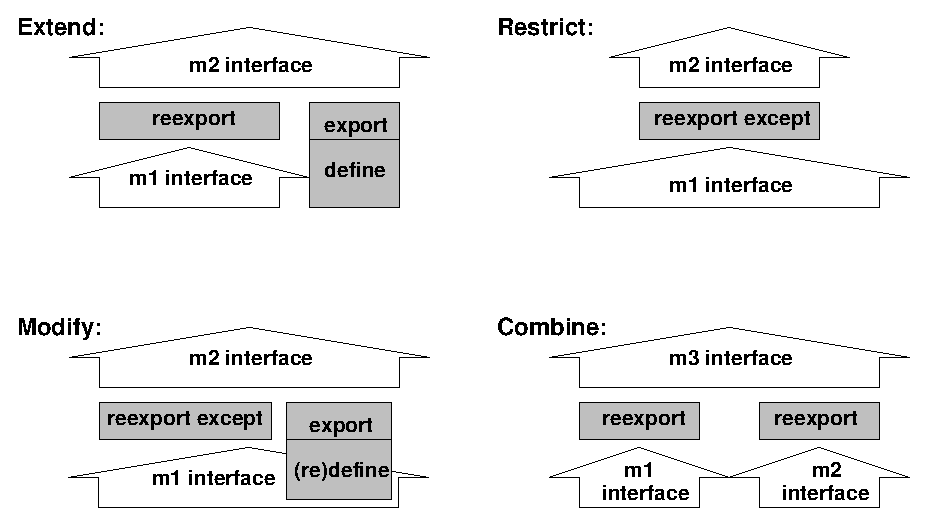
\includegraphics{reexport.eps}
\end{center}
\caption{Making modules from modules with reexport}
\label{reexport}
\end{figure}


%----------------------------------------------------------------------
\subsection{Modules and Source Files}
\index{source files}
%----------------------------------------------------------------------

When a source file contains no module directives, it becomes part of
the module from which its compilation was invoked.  This makes it
possible to write small programs without caring about modules. 
However, serious applications should be structured into modules. 

Often it is the most appropriate to have one file per module and to
have the file name match the module name.

It is however possible to have several modules in one file, e.g.\ a
main module and one or more auxiliary modules - in that
case the name of the main module should match the filename.
Every module-directive in the file marks the end of the previous
module and the start of the next one.

It is also possible to spread the contents of a module over several
files. In this case, there should be a main file whose filename
matches the module name, and the other files should be referenced
from the main file using the \bipref{include/1}{../bips/kernel/directives/include-1.html} directive, e.g.
\begin{quote}\begin{verbatim}
:- module(bigmodule).
:- include(part1).
:- include(part2).
\end{verbatim}\end{quote}



%----------------------------------------------------------------------
\subsection{Tools and Caller Modules}
%----------------------------------------------------------------------

\subsubsection{Tools}
\index{Tools}
\index{procedure!tool}
\label{tools}
There are predicates in a modular system that need to know from which
module they were called (since this may be different from the module
in which they were defined).
\index{meta-predicates}
The most common case is where a predicate is a meta-predicate,
i.e.\ a predicate that has another goal or predicate name as an argument.
Other cases are I/O predicates - they need to be executed in a
certain module context in order to obey the correct syntax of this module.
In {\eclipse}, such predicates that need to know their caller module
are called {\bf tool} predicates\footnote{
    Many Prolog systems call them meta-predicates.}.

Tool predicates must be declared.  As a consequence, the system will
automatically add a {\bf caller module} argument whenever such a tool
predicate is called.

Consider for example a predicate that calls another predicate twice.
\index{twice/1}
The naive version of this predicate looks like
\begin{quote} \begin{verbatim}
twice(Goal) :-
    call(Goal),
    call(Goal).
\end{verbatim} \end{quote}
As long as no modules are involved, this works fine.
Now consider the situation where the definition of twice/1 and a
call of twice/1 are in two different modules:
\begin{quote} \begin{verbatim}
:- module(stuff).
:- export twice/1.
twice(Goal) :-
    call(Goal),
    call(Goal).

:- module(main).
:- import stuff.

top :- twice(hello).

hello :- writeln(hi).
\end{verbatim} \end{quote}
This will not work because hello/0 is only visible in module main
and an attempt to call it from within twice/1 in module stuff will
raise an error. The solution is to declare twice/1 as a tool and
change the code as follows:
\begin{quote} \begin{verbatim}
:- module(stuff).
:- export twice/1.
:- tool(twice/1, twice/2).
twice(Goal, Module) :-
    call(Goal)@Module,
    call(Goal)@Module.
\end{verbatim} \end{quote}
What happens now is that the call to twice/1 in module main
\begin{quote} \begin{verbatim}
..., twice(hello), ...
\end{verbatim} \end{quote}
is effectively replaced by the system with a call to twice/2 where
the additional argument is the module in which the call occurs:
\begin{quote} \begin{verbatim}
..., twice(hello, main), ...
\end{verbatim} \end{quote}
This caller module is then used by twice/2 to execute
\begin{quote} \begin{verbatim}
..., call(hello)@main, ...
\end{verbatim} \end{quote}
The 
\biprefnoidx{call(Goal)@Module}{../bips/kernel/control/A-2.html}
\index{\atsym/2} construct means that the call is supposed to happen
{\em in the context} of module main.


The debugger trace shows what happens:
\begin{quote} \begin{verbatim}
[main 5]: top.
  (1) 1 CALL  top
  (2) 2 CALL  twice(hello)
  (3) 3 CALL  twice(hello, main)
  (4) 4 CALL  call(hello) @ main
  (5) 5 CALL  call(hello)
  (6) 6 CALL  hello
S (7) 7 CALL  writeln(hi)
hi
S (7) 7 EXIT  writeln(hi)
  (6) 6 EXIT  hello
  ...
\end{verbatim} \end{quote}

One complication that can arise when you use tools is that the compiler
must know that a predicate is a tool in order to properly compile
a call to the tool.
If the call occurs textually before the tool
declaration,  this will therefore give rise to an
{\bf inconsistent tool redefinition} error.
The
\bipref{tool/2}{../bips/kernel/modules/tool-2.html}
declaration must therefore occur before any call to the tool.


\subsubsection{System Tools}
\index{tool!system}
Many of the system built-in predicates are in fact tools, e.g.
\bipref{read/1}{../bips/kernel/ioterm/read-1.html},
\bipref{write/1}{../bips/kernel/ioterm/write-1.html},
\bipref{record/2}{../bips/kernel/record/record-2.html},
\bipref{compile/1}{../bips/kernel/database/compile-1.html}, etc.
All predicates which handle modular items must be tools
so that they know from which module they have been called.
In case that the built-in predicate has to be executed in
a different module (this is very often the case inside
user tool predicates), the 
\biptxtref{@ /2}{\atsym /2}{../bips/kernel/control/A-2.html}
construct must be used, e.g.
\begin{quote}\begin{verbatim}
current_predicate(P) @ SomeModule
\end{verbatim}\end{quote}


%----------------------------------------------------------------------
\subsection{Lookup Module vs Caller Module}
\index{lookup module}
\index{caller module}
%----------------------------------------------------------------------

The following table summarises the different call patterns with and
without module specifications.
There are only two basic rules to remember:
\begin{itemize}
\item \bipref{: /2}{../bips/kernel/control/N-2.html}
	specifies the {\bf lookup module} (to find the definition)
\item \biprefnoidx{@ /2}{../bips/kernel/control/A-2.html}
% need a separate index entry because latex evaluates \atsym too early
% inside \bipref
\index{\atsym/2} 
	specifies the {\bf caller module} (to know the context)
\end{itemize}

\begin{tabular}{|p{5cm}|p{4cm}|p{4cm}|}
\hline
Call inside module(m)	& Module where definition of twice/1 is looked up
	    & Caller module argument added to twice/1 \\
\hline
..., twice(X), ...		&  m &  m \\
..., lm : twice(X), ...		& lm &  m \\
..., twice(X) @ cm, ...		&  m & cm \\
..., lm : twice(X) @ cm, ...	& lm & cm \\
..., call(twice(X)) @ cm, ...	& cm & cm \\
\hline
\end{tabular}


%----------------------------------------------------------------------
\subsection{The Module Interface}
%----------------------------------------------------------------------
The primitive 
\bipref{current_module/1}{../bips/kernel/modules/current_module-1.html}
can be used to check for the existence of a module, or to enumerate
all currently defined modules.

Further details about existing modules can be retrieved using
\index{properties!module}
\bipref{get_module_info/3}{../bips/kernel/modules/get_module_info-3.html},
in particular information about the module's interface, what other
modules it uses and whether it is locked (see~\ref{locking}).


%----------------------------------------------------------------------
\subsection{Module-related Predicate Properties}
%----------------------------------------------------------------------
Information about a predicate's properties can be retrieved using the 
\index{properties!predicate}
\bipref{get_flag/3}{../bips/kernel/database/get_flag-3.html} primitive
or printed using \bipref{pred/1}{../bips/kernel/env/pred-1.html}.
The module-related predicate properties are
\begin{description}
\item[defined]
	(on/off) indicates whether code for the predicate has already
	been compiled. If not, only a declaration was encountered.
\item[definition_module]
	(an atom) the module where the predicate is defined.
\item[visibility]
	(local/exported/reexported/imported) indicates the visibility
	of the predicate in the caller module.
\item[tool]
	(on/off) indicates whether the predicate has been declared a tool.
\end{description}
For tool predicates, 
\bipref{tool_body/3}{../bips/kernel/modules/tool_body-3.html}
can be used to retrieve the predicate it maps to when the module
argument is added.

To get information about a predicate visible in a different module,
use for instance
\begin{quote}\begin{verbatim}
    get_flag(p/3, visibility, V) @ othermodule
\end{verbatim}\end{quote}

%----------------------------------------------------------------------
\section{Less Common Topics}
%----------------------------------------------------------------------

%----------------------------------------------------------------------
\subsection{Modules Using Other Languages}
%----------------------------------------------------------------------

Modules created with the \bipref{module/1}{../bips/kernel/modules/module-1.html} directive automatically import
\index{language}
\index{eclipse_language}
the module {\tt eclipse_language},  which provides the standard set
of {\eclipse} built-in predicates. 
To create a module that uses a different language dialect, use
\bipref{module/3}{../bips/kernel/modules/module-3.html}.
For instance
\begin{quote}\begin{verbatim}
:- module(mystdcode, [], iso).
\end{verbatim}\end{quote}
creates a module in which you can use ISO Standard Prolog\footnote{to the
extent implemented by {\eclipse}'s compatibility library},
but not all of {\eclipse}'s usual language features.
Note that the third argument (here {\tt iso}) simply
specifies a library which implements the desired language,
so new languages can be added easily.


%----------------------------------------------------------------------
\subsection{Creating and Erasing Modules at Runtime}
%----------------------------------------------------------------------
\begin{sloppypar}
A module can also be created explicitly by a running program with
\bipref{create_module/1}{../bips/kernel/modules/create_module-1.html} or
\bipref{create_module/3}{../bips/kernel/modules/create_module-3.html}
and erased with
\bipref{erase_module/1}{../bips/kernel/modules/erase_module-1.html}. 
The latter should be used with care, erasing a module while a
predicate defined in that module is being executed can provoke
unpredictable results. The same holds for trying to erase essential
system modules.
\end{sloppypar}


%----------------------------------------------------------------------
\subsection{Initialization and Finalization}
\label{initfini}
\index{initialization}
\index{finalization}
%----------------------------------------------------------------------
Sometimes modules have global state which needs to be initialised
or finalised. For this purpose, modules can have
\begin{description}
\item[Local Initialization Goals:]
these are specified as
\begin{quote}\begin{verbatim}
:- local initialization(Goal).
\end{verbatim}\end{quote}
and are executed just after the module containing them has been loaded.
\item[Exported Initialization Goals:]
these are specified as
\begin{quote}\begin{verbatim}
:- export initialization(Goal).
\end{verbatim}\end{quote}
and are executed whenever the module containing the declaration gets
imported into another module. The call will happen in the context of
the importing module.
\item[Finalization Goals:]
these are specified as
\begin{quote}\begin{verbatim}
:- local finalization(Goal).
\end{verbatim}\end{quote}
and are executed just before the module containing them gets erased.
Modules can get erased either explicitly through
\bipref{erase_module/1}{../bips/kernel/modules/erase_module-1.html} 
or implicitly when the module is re-compiled, or when the {\eclipse}
session is exited.  Finalization goals should not do any I/O because
in the case of an embedded ECLiPSe, I/O may no longer be available at
finalization time.

\end{description}

%----------------------------------------------------------------------
\subsection{Locking Modules}
\label{locking}
\index{locking}
%----------------------------------------------------------------------
By default, {\eclipse} does not strictly enforce the hiding of
module internals. This facilitates program development as is makes
it possible to inspect and trace without being too concerned about module
boundaries. E.g.\ you can set a spy point on a local predicate p/3
in module othermod by calling:
\begin{quote}\begin{verbatim}
:- spy(p/3)@othermod.
\end{verbatim}\end{quote}
Once a module implementation is stable and there is a need for privacy,
it is possible to {\em lock} a module. Locking makes it impossible
to access internal, local items from outside the module. Of course,
the module can still be used though its interface.
The built-in predicates related to locking are
\bipref{lock/0}{../bips/kernel/modules/lock-0.html} which provides
a definitive lock,
\bipref{lock_pass/1}{../bips/kernel/modules/lock_pass-1.html}
which allows subsequent unlocking using a password (
\bipref{unlock/2}{../bips/kernel/modules/unlock-2.html}),
and
\bipref{get_module_info/3}{../bips/kernel/modules/get_module_info-3.html}
which allows to check whether a module is locked.
\bipref{lock/0}{../bips/kernel/modules/lock-0.html} and
\bipref{lock_pass/1}{../bips/kernel/modules/lock_pass-1.html} are
usually used as a directive in the source file of the module to be locked.

%HEVEA\cutend

% BEGIN LICENSE BLOCK
% Version: CMPL 1.1
%
% The contents of this file are subject to the Cisco-style Mozilla Public
% License Version 1.1 (the "License"); you may not use this file except
% in compliance with the License.  You may obtain a copy of the License
% at www.eclipse-clp.org/license.
%
% Software distributed under the License is distributed on an "AS IS"
% basis, WITHOUT WARRANTY OF ANY KIND, either express or implied.  See
% the License for the specific language governing rights and limitations
% under the License.
%
% The Original Code is  The ECLiPSe Constraint Logic Programming System.
% The Initial Developer of the Original Code is  Cisco Systems, Inc.
% Portions created by the Initial Developer are
% Copyright (C) 1995 - 2006 Cisco Systems, Inc.  All Rights Reserved.
%
% Contributor(s):
%
% END LICENSE BLOCK
%
% @(#)umsarith.tex	1.8 95/03/17
%
%
%
% REL      DATE      AUTHOR             DESCRIPTION
% 2.10     080489    David Miller       Begin work on new arithmetic chapter
%                                       based on old builtins chapter.
%          250489    Joachim Schimpf    Modified for inline compiled arithmetic
%
\chapter{Arithmetic Evaluation\label{chaparith}}
\index{arithmetic}
%HEVEA\cutdef[1]{section}

\section{Built-Ins to Evaluate Arithmetic Expressions}
\index{arithmetic!built-ins}\index{built-ins!arithmetic}
Unlike other languages, Prolog usually interprets an arithmetic expression like
\notation{3 + 4} as a compound term with functor \notation{+} and two arguments.
Therefore a query like \notation{3 + 4 = 7} fails because a compound term does
not
unify with a number. The evaluation of an arithmetic expression has to be
explicitly requested by using one of the built-ins described below.

\index{comparison!arithmetic}\index{arithmetic!comparison}%
\index{arithmetic!built-ins!comparison}\index{built-ins!arithmetic!comparison}
The basic predicate for evaluating an arithmetic expression is
\bipref{is/2}{../bips/kernel/arithmetic/is-2.html}.
Apart from that only the 6 arithmetic comparison predicates evaluate
arithmetic expressions automatically.

\begin{quote}
\begin{description}
\item[\pattern{Result} is \pattern{Expression}]\indextt{is/2}
\about{Expression} is a valid arithmetic expression and \about{Result}
is an uninstantiated variable or a number.
The system evaluates \about{Expression} which yields a numeric result.
This result is then unified with \about{Result}.
An error occurs if \about{Expression} is not a valid arithmetic expression or
if the evaluated value and \about{Result} are of different types.

\item[\pattern{Expr1} $<$ \pattern{Expr2}]\indextt{</2}
succeeds if (after evaluation and type coercion) \about{Expr1} is less than
\about{Expr2}.

\item[\pattern{Expr1} $>=$ \pattern{Expr2}]\indextt{>=/2}
succeeds if (after evaluation and type coercion) \about{Expr1} is greater or
equal to \about{Expr2}.

\item[\pattern{Expr1} $>$ \pattern{Expr2}]\indextt{>/2}
succeeds if (after evaluation and type coercion) \about{Expr1} is greater than
\about{Expr2}.

\item[\pattern{Expr1} $=<$ \pattern{Expr2}]\indextt{=</2}
succeeds if (after evaluation and type coercion) \about{Expr1} is less or equal
to \about{Expr2}.

\item[\pattern{Expr1} =:= \pattern{Expr2}]\indextt{=:=/2}
succeeds if (after evaluation and type coercion) \about{Expr1} is equal to
\about{Expr2}.

\item[\pattern{Expr1} =\bsl= \pattern{Expr2}]%
\index{=\bsl=/2@\notation{=}\bsl\notation{=/2}}
succeeds if (after evaluation and type coercion) \about{Expr1} is not equal to
\about{Expr2}.
\end{description}
\end{quote}


\subsection{Arithmetic Evaluation vs Arithmetic Constraint Solving}

This chapter deals purely with the evaluation of arithmetic expressions
containing numbers. No uninstantiated variables must occur within the
expressions at the time they are evaluated. This is exactly like
arithmetic evaluation in procedural languages.

As opposed to that, in arithmetic constraint solving one can state
equalities and inequalities involving variables, and a constraint
solver tries to find values for these variables which satisfy these
constraints. Note that {\eclipse} uses the same syntax in both cases,
but different implementations providing different solving capabilities.
See the chapter \chapname{Common Solver Interface} in the
\ahref{../libman/libman.html}{Constraint Library Manual} for an overview.


\section{Numeric Types and Type Conversions}
\index{arithmetic!types}\index{types!arithmetic}
{\eclipse} distinguishes four types of numbers: \defnotionni{integers},
\defnotionni{rationals}, \defnotionni{floats} and \defnotionni{bounded reals}.
% we might have bounded integers at some point...

\subsection{Integers\label{intrep}}
\index{integers}
\index{bignum}
\index{type!integer}
The magnitude of integers is only limited by your available
memory. However, integers that fit into the word size of your computer are
represented more efficiently (this distinction is invisible to the user).
Integers are written in decimal notation or in base notation, for example:
\begin{quote}
\begin{verbatim}
0  3  -5  1024  16'f3ae  0'a  15511210043330985984000000
\end{verbatim}
\end{quote}

Note that integer range is unlimited if {\eclipse} was compiled with
bignum support. Otherwise, integers are restricted to that representable
in a machine word, and  \notation{max_integer flag} of
\bipref{get_flag/2}{../bips/kernel/env/get_flag-2.html}
returns the maximum integer value.

\subsection{Rationals}
\index{rational numbers}
\index{type!rational}
Rational numbers implement the corresponding mathematical domain,
i.e., ratios of two integers (numerator and denominator).
{\eclipse} represents rationals in a canonical form where the
greatest common divisor of numerator and denominator is 1 and the
denominator is positive. Rational constants are written as numerator
and denominator separated by an underscore, e.g.,
\begin{quote}
\begin{verbatim}
1_3  -30517578125_32768  0_1
\end{verbatim}
\end{quote}
Rational arithmetic is arbitrarily precise. When the global flag
\index{global flag!prefer_rationals}
\notationidx{prefer_rationals} is set, the system uses rational arithmetic
wherever possible. In particular, dividing two integers then yields a precise
rational rather than a float result.

Rationals are supported if {\eclipse} is compiled with bignum support.
If rationals are not supported, a type error will be raised when a rational is
required.

\subsection{Floating Point Numbers}
\index{floating point numbers}
\index{type!float}
Floating point numbers conceptually correspond to the mathematical
domain of real numbers, but are not precisely represented.
Floats are written with decimal point and/or an exponent, e.g.,
\begin{quote}
\begin{verbatim}
0.0  3.141592653589793  6.02e23  -35e-12  -1.0Inf
\end{verbatim}
\end{quote}
{\eclipse} uses double precision floats\footnote{%
  {\eclipse} versions older than 5.5 optionally supported single precision
  floats. This is no longer the case.}.


\subsection{Bounded Real Numbers}
\index{bounded reals}
\index{breal}
\index{type!breal}
It is a well known problem that floating point arithmetic suffers
from rounding errors.
To provide safe arithmetic over the real numbers, {\eclipse}
also implements bounded reals\footnote{%
  We have chosen to use the term \about{bounded real} rather than
  \about{interval} in order to avoid confusion with interval variables
  as used in the interval arithmetic constraint solvers}.
A bounded real consists of a pair of floating point numbers
which constitute a safe lower and upper bound for the real number that
is being represented. Bounded reals are written as two floating point
numbers separated by two underscores, e.g.,
\begin{quote}
\begin{verbatim}
-0.001__0.001  3.141592653__3.141592654  1e308__1.0Inf
\end{verbatim}
\end{quote}
A bounded real is a representation for a real number that definitely lies
somewhere between the two bounds, but the exact value cannot be determined\
\footnote{%
  This is in contrast to a floating point number, which represents
  a real number which lies somewhere in the vicinity of the float}.
Bounded reals are usually not typed in by the user, they are normally
the result of a computation or type coercion.

All computations with bounded reals give safe results, taking rounding
errors into account. This is achieved by doing \Index{interval arithmetic}
on the bounds and rounding the results outwards. The resulting
bounded real is then guaranteed to enclose the true real result.

Computations with floating point values result in uncertainties
about the correct result. Bounded reals make this uncertainty
explicit. A consequence of this is that sometimes it is conceptually
not possible to decide whether two bounded reals are identical or not.
This occurs when the bounds of the compared intervals overlap.
In this case, the arithmetic comparisons leave a (ground) delayed goal
behind which can then be inspected by the user to decide whether the
match is considered close enough. The syntactical comparisons like
\bipref{=/2}{../bips/kernel/termcomp/E-2.html} and
\bipref{==/2}{../bips/kernel/termcomp/EE-2.html} treat bounded reals
simply as a pair of bounds, and consider them equal when the bounds are
equal.


\subsection{Type Conversions}
Note that numbers of different types never unify, e.g., 3, 3_1, 3.0
and 3.0__3.0 are all different.
Use the arithmetic comparison predicates when you want to
compare numeric values.
When numbers of different types occur as arguments of an arithmetic
operation or comparison, the types are first made equal by converting
to the more general of the two types, i.e., the rightmost one in the sequence
\begin{quote}
integer $\rightarrow$ rational $\rightarrow$ float $\rightarrow$ bounded real
\end{quote}
The operation or comparison is then carried out with this type and the
result is of this type as well, unless otherwise specified.
Beware of the potential loss of precision in the
rational $\rightarrow$ float conversion!
Note that the system never does automatic conversions in the opposite direction.
Such conversion must be programmed explicitly using the
\biptxtref{integer}{integer/2}{../bips/kernel/arithmetic/integer-2.html},
\biptxtref{rational}{rational/2}{../bips/kernel/arithmetic/rational-2.html},
\biptxtref{float}{float/2}{../bips/kernel/arithmetic/float-2.html} and
\biptxtref{breal}{breal/2}{../bips/kernel/arithmetic/breal-2.html}
functions.

\section{Arithmetic Functions}
\index{arithmetic!functions}\index{functions!arithmetic}
\subsection{Predefined Arithmetic Functions}
\index{arithmetic!predefined arithmetic functions}
The following predefined arithmetic functions are available.
\about{E}, \about{E1} and \about{E2} stand for
arbitrary arithmetic expressions.

\vspace{2mm}
\noindent
{\small
\begin{tabular}{l l l l}
Function & Description & Argument Types & Result Type \\
\hline
+ E        & unary plus & number & number \\
-- E       & unary minus & number & number \\
abs(E)    & absolute value & number & number \\
sgn(E)    & sign value & number & integer \\
floor(E)   & round down to integral value & number & number \\
ceiling(E) & round up to integral value & number & number \\
round(E)   & round to nearest integral value & number & number \\
truncate(E) & truncate to integral value & number & number \\
E1 + E2    & addition & number $\times$ number & number \\
E1 -- E2   & subtraction & number $\times$ number & number \\
E1 * E2    & multiplication & number $\times$ number & number \\
E1 / E2    & division & number $\times$ number & see below \\
E1 // E2   & integer division (truncate) & integer $\times$ integer & integer \\
E1 rem E2  & integer remainder & integer $\times$ integer & integer \\
E1 div E2  & integer division (floor) & integer $\times$ integer & integer \\
E1 mod E2  & integer modulus & integer $\times$ integer & integer \\
gcd(E1,E2) & greatest common divisor & integer $\times$ integer & integer \\
lcm(E1,E2) & least common multiple & integer $\times$ integer & integer \\
E1 \char`\^\ E2 & power operation & number $\times$ number & number \\
min(E1,E2) & minimum of 2 values & number $\times$ number & number \\
max(E1,E2) & maximum of 2 values & number $\times$ number & number \\
\verb:\: E & bitwise complement & integer & integer \\
E1 \verb:/\: E2  & bitwise conjunction & integer $\times$ integer & integer \\
E1 \verb:\/: E2 & bitwise disjunction & integer $\times$ integer & integer \\
xor(E1,E2) & bitwise exclusive disjunction & integer $\times$ integer & integer \\
E1 $>>$ E2 & shift E1 right by E2 bits & integer $\times$ integer & integer \\
E1 $<<$ E2 & shift E1 left by E2 bits & integer $\times$ integer & integer \\
sin(E)     & trigonometric function & number & real \\
cos(E)     & trigonometric function & number & real \\
tan(E)     & trigonometric function & number & real \\
asin(E)    & trigonometric function & number & real \\
acos(E)    & trigonometric function & number & real \\
atan(E)    & trigonometric function & number & real \\
atan(E1,E1) & trigonometric function & number $\times$ number & real \\
exp(E)     & exponential function \( e^{x} \) & number & real \\
ln(E)      & natural logarithm & number & real \\
sqrt(E)    & square root & number & real \\
pi         & the constant pi = 3.1415926...  & --- & float \\
e          & the constant e = 2.7182818... & --- & float \\
fix(E)     & convert to integer (truncate) & number & integer \\
integer(E) & convert to integer (exact) & number & integer \\
float(E)   & convert to float & number & float \\
breal(E)   & convert to bounded real & number & breal \\
rational(E)   & convert to rational & number & rational \\
rationalize(E) & convert to rational & number & rational \\
numerator(E)   & extract numerator of a  rational & integer or rational &
                 integer \\
denominator(E)   & extract denominator of a rational & integer or rational &
                   integer \\
sum(L)   & sum of list elements & list & number \\
min(L)   & minimum of list elements & list & number \\
max(L)   & maximum of list elements & list & number \\
eval(E)   & evaluate runtime expression & term & number \\
\end{tabular}
}
\vspace{2mm}
\vfill       %<<<<<<<<<<<
\pagebreak   %<<<<<<<<<<<

\noindent
Argument types other than specified yield a type error.
As an argument type, \about{number} stands for \about{integer},
\about{rational}, \about{float} or \about{breal} with the type conversions as
specified above.
As a result type, \about{number} stands for
\emph{the more general of the argument types}, and \about{real} stands for
\about{float} or \about{breal}.
The division operator \notation{/} yields either a rational or a float result,
depending on the value of the global flag
\notationidx{prefer_rationals}.%
\index{global flag!prefer_rationals}\index{arithmetic!prefer_rationals}
The same is true for the result of \char`\^\ if an integer is raised to
a negative integral power.

The integer division \notation{//} rounds the result towards zero (truncates),
while the \notation{div} division rounds towards negative infinity (floor).
Each division function is paired with a corresponding remainder function:
(\notation{rem} computes the remainder corresponding to \notation{//}, and
\notation{mod}
computes the remainder corresponding to \notation{div}\
\footnote{%
  Caution: In {\eclipse} versions up to 5.8, \notation{mod} was the
  remainder corresponding to \notation{//}, i.e., behaved like \notation{rem}}.
The remainder results differ only in the case where the two arguments
have opposite signs.  The relationship between them is as follows:
\begin{quote}
\begin{verbatim}
X =:= (X rem Y) + (X // Y) * Y
X =:= (X mod Y) + (X div Y) * Y
\end{verbatim}
\end{quote}
This table gives an overview:
\begin{quote}
\begin{verbatim}
      10 x 3   -10 x 3   10 x -3   -10 x -3

//       3        -3       -3          3
rem      1        -1        1         -1
div      3        -4       -4          3
mod      1         2       -2         -1
\end{verbatim}
\end{quote}

\subsection{Evaluation Mechanism}
\index{arithmetic!expressions}

An arithmetic expression is a Prolog term that is made up of variables,
numbers, atoms and compound terms, e.g.,
\begin{quote}
\begin{verbatim}
3 * 1.5 + Y / sqrt(pi)
\end{verbatim}\end{quote}
Compound terms are evaluated by first evaluating their arguments and then
calling the corresponding evaluation predicate.
The evaluation predicate associated with a compound term
 \notation{func(a_1,..,a_n)}
is the predicate \predspec{func/}$(n+1)$. It receives
\notation{a_1},..,\notation{a_n} as its first
\about{n} arguments and returns a numeric result as its last argument.
This result is then used in the arithmetic computation.
For instance, the expression above would be evaluated by the goal sequence
\begin{quote}
\begin{verbatim}
*(3,1.5,T1), sqrt(3.14159,T2), /(Y,T2,T3), +(T1,T3,T4)
\end{verbatim}\end{quote}
where \about{T1}, \about{T2} etc. are auxiliary variables created by the system
to hold
intermediate results.

Although this evaluation mechanism is usually transparent to the user, it
becomes visible when errors occur, when subgoals are delayed, or
when inline-expanded code is traced.

\subsection{User Defined Arithmetic Functions}
\index{arithmetic!user defined arithmetic}
This evaluation mechanism outlined above is not restricted to the
predefined arithmetic functions shown in the table.
In fact it works for all atoms and compound terms.
It is therefore possible to define a new arithmetic operation by
just defining an evaluating predicate:
\index{factorial function}
\begin{quote}
\begin{verbatim}
[eclipse 1]: [user].
 :- op(200, yf, !).             % let's have some syntaxtic sugar
 !(N, F) :- fac(N, 1, F).
 fac(0, F0, F) :- !, F=F0.
 fac(N, F0, F) :- N1 is N-1, F1 is F0*N, fac(N1, F1, F).
 user       compiled traceable 504 bytes in 0.00 seconds

yes.
[eclipse 2]: X is 23!.       % calls !/2

X = 25852016738884976640000
yes.
\end{verbatim}
\end{quote}
Note that this mechanism is not only useful for user-defined predicates, but
can also be used to call {\eclipse} built-ins inside arithmetic expressions,
e.g.,
\begin{quote}
\begin{verbatim}
T is cputime - T0.
L is string_length("abcde") - 1.
\end{verbatim}\end{quote}
which call \bipref{cputime/1}{../bips/kernel/opsys/cputime-1.html} and
\bipref{string_length/2}{../bips/kernel/stratom/string_length-2.html}
respectively.
Any predicate that returns a number as its last argument
can be used in a similar manner.

However there is a difference compared to the evaluation of the predefined
arithmetic functions (as listed in the table above):
The arguments of the user-defined arithmetic expression are \emph{not
evaluated} but passed unchanged to the evaluating predicate.
For example, the expression \notation{twice(3+4)} is transformed into the goal
\notation{twice(3+4, Result)} rather than \notation{twice(7, Result)}.
This makes sense because otherwise it would not be possible to pass
any compound term to the predicate.
If evaluation is wanted, the user-defined predicate can explicitly call
\bipref{is/2}{../bips/kernel/arithmetic/is-2.html} or use \predspec{eval/1}.

\subsection{Runtime Expressions}
In order to enable efficient compilation of arithmetic expressions,
{\eclipse} requires that variables in compiled arithmetic expressions
must be bound to numbers at runtime, not symbolic expressions.
For example, in the following code \predspec{p/1} will only work when called
with a
numerical argument, else it will raise error 24:
\begin{quote}
\begin{verbatim}
p(Number) :- Res is 1 + Number, ...
\end{verbatim}
\end{quote}
To make it work even when the argument gets bound to a symbolic expression
at runtime, use \predspec{eval/1} as in the following example:
\begin{quote}
\begin{verbatim}
p(Expr) :- Res is 1 + eval(Expr), ...
\end{verbatim}
\end{quote}
If the expression is the only argument of \predspec{is/2}, the \predspec{eval/1}
may be omitted.


\section{Low Level Arithmetic Builtins}
The low level builtins (like
\txtbipref{+/3}{+/3}{../bips/kernel/arithmetic/P-3.html},
\bipref{sin/2}{../bips/kernel/arithmetic/sin-2.html} etc.)
which are used to evaluate
the predefined arithmetic functions can also be called directly,
but this is not recommended for portability reasons.
\index{compiler!arithmetic}
Moreover, there is no need to use them directly since the {\eclipse} compiler
will transform all arithmetic expressions into calls to the corresponding
low level builtins.

\section{The Multi-Directional Arithmetic Predicates}%
A drawback of arithmetic using
\bipref{is/2}{../bips/kernel/arithmetic/is-2.html} is that the right hand side
must
be fully instantiated at evaluation time.
Often it is desirable to have predicates that define true logic
relationships between their arguments like ``\about{Z} is the sum of \about{X}
and \about{Y}''.
For integer addition and multiplication this is provided as:
\begin{quote}
\begin{description}
\item[succ(X, Y)]\indextt{succ/2}
True if \about{X}and \about{Y} are natural numbers, and \about{Y} is one greater
than \about{X}.
At most one of \about{X}, \about{Y} can be a variable.

\item[plus(X, Y, Z)]\indextt{plus/3}
True if the sum of \about{X} and \about{Y} is \about{Z}. At most one of
\about{X}, \about{Y}, \about{Z} can be a variable.

\item[times(X, Y, Z)]\indextt{times/3}
True if the product of \about{X} and \about{Y} is \about{Z}. At most one of
\about{X}, \about{Y}, \about{Z} can be a variable.

\end{description}
\end{quote}

These predicates work only with integer arguments but any single argument
can be a variable which is then instantiated so that the relation holds.
If more than one argument is uninstantiated, an instantiation fault is produced.

Note that if one of the first two arguments is a variable,
a solution doesn't necessarily exist. For example, the following goal has
no integer solution :
\begin{quote}
\begin{verbatim}
[eclipse 1]: times(2, X, 3).

no (more) solution.
\end{verbatim}\end{quote}

Since any one of the arguments of these two predicates can be a variable,
it does not make much sense to use them in arithmetic expressions
where always the first arguments are taken as input and the last
one as output.

\section{Arithmetic and Coroutining}
\index{arithmetic!coroutining}
\index{coroutining!arithmetic}
\index{delay!arithmetic}
\label{arithdelay}

Arithmetic comparisons can be delayed until their arguments are
instantiated instead of generating an instantiation fault by passing the
comparison to the suspend solver (see section~\ref{suspendsolver}). This
gives a form of coroutining.

%HEVEA\cutend


% BEGIN LICENSE BLOCK
% Version: CMPL 1.1
%
% The contents of this file are subject to the Cisco-style Mozilla Public
% License Version 1.1 (the "License"); you may not use this file except
% in compliance with the License.  You may obtain a copy of the License
% at www.eclipse-clp.org/license.
%
% Software distributed under the License is distributed on an "AS IS"
% basis, WITHOUT WARRANTY OF ANY KIND, either express or implied.  See
% the License for the specific language governing rights and limitations
% under the License.
%
% The Original Code is  The ECLiPSe Constraint Logic Programming System.
% The Initial Developer of the Original Code is  Cisco Systems, Inc.
% Portions created by the Initial Developer are
% Copyright (C) 1996 - 2006 Cisco Systems, Inc.  All Rights Reserved.
%
% Contributor(s):
%
% END LICENSE BLOCK
%
% @(#)umsarrays.tex     1.4
%

\chapter{Non-logical Storage and References}
\label{chaparrays}
%HEVEA\cutdef[1]{section}

%----------------------------------------------------------------------
\section{Introduction}
%----------------------------------------------------------------------

This chapter describes primitives that allow one to break the normal logic
programming rules in two ways:
\begin{itemize}
\item information can be \emph{saved across logical failures} and backtracking;
\item information can be accessed by \emph{naming} rather than by argument
  passing.
\end{itemize}
Obviously, these facilities must be used with care and should always
be encapsulated in an interface that provides logical semantics.

ECLiPSe provides several facilities to store information across
backtracking.  The following table gives an overview.  If at all
possible, the handle-based facilities (bags, shelves and stores) should be
preferred because they lead to cleaner, reentrant code (without global
state) and reduce the risk of memory leaks.

\vspace{2mm}
\begin{center}
\begin{tabular}{l|l l l}
Facility & Type & Access & See \\
\hline
shelves&                array&          by handle&      shelf_create/2,3 \\
bags&                   unordered bag&  by handle&      bag_create/1 \\
stores&                 hash table&     by handle&      store_create/1 \\
named shelves&          array&          by name&        shelf/2 \\
named stores&           hash table&     by name&        store/1 \\
non-logical variables&  single cell&    by name&        variable/1 \\
non-logical arrays&     array&          by name&        array/1,2 \\
records&                ordered list&   by name&        record/1,2 \\
dynamic predicates&     ordered list&   by name&        dynamic/1, assert/1 \\
\end{tabular}
\end{center}
\vspace{2mm}

\index{reference}
\index{global reference}
The other facility described here, \emph{Global References}, does not store
information across failure, but provides a means to give a name to
an otherwise logical data structure. See section \ref{globrefs}.


%----------------------------------------------------------------------
\section{Bags}
%----------------------------------------------------------------------

A bag is an anonymous object which can be used to store
information across failures.
A bag is unordered and untyped. Any {\eclipse} term can be stored in a bag.
Bags are referred to by a handle.
An empty bag is created using
\bipref{bag_create/1}{../bips/kernel/storage/bag_create-1.html},
data is stored in the bag by invoking
\bipref{bag_enter/2}{../bips/kernel/storage/bag_enter-2.html},
and the stored data can be retrieved as a list with
\bipref{bag_retrieve/2}{../bips/kernel/storage/bag_retrieve-2.html} or
\bipref{bag_dissolve/2}{../bips/kernel/storage/bag_dissolve-2.html}.

A typical application is the
implementation of the \predspec{findall/3} predicate or similar functionality.
As opposed to the use of \predspec{record/2} or \predspec{assert/1}, the
solution using
bags is more efficient, more robust, and trivially reentrant.
\begin{verbatim}
    simple_findall(Goal, Solutions) :-
        bag_create(Bag),
        (
            call(Goal),
            bag_enter(Bag, Goal),
            fail
        ;
            true
        ),
        bag_dissolve(Bag, Solutions).
\end{verbatim}


%----------------------------------------------------------------------
\section{Shelves}
%----------------------------------------------------------------------

A \defnotion{shelf} is an anonymous object which can be used to store information
across failures.  A typical application is counting of solutions,
keeping track of the best solution, aggregating information across
multiple solutions, etc.

A shelf is an object with multiple slots whose contents survive
backtracking.  The content of each slot can be set and retrieved
individually, or the whole shelf can be retrieved as a term.

Shelves are referred to by handle, not by name, so they make it easy
to write robust, reentrant code.  A shelf disappears when the system
backtracks over its creation, when the shelf handle gets garbage
collected, or when it is explicitly destroyed.

A shelf is initialized using
\bipref{shelf_create/2}{../bips/kernel/storage/shelf_create-2.html} or
\bipref{shelf_create/3}{../bips/kernel/storage/shelf_create-3.html}.
Data is stored in the slots (or the shelf as a whole) with
\bipref{shelf_set/3}{../bips/kernel/storage/shelf_set-3.html}
and retrieved with
\bipref{shelf_get/3}{../bips/kernel/storage/shelf_get-3.html}.

Example: Counting how many solutions a goal has:
\begin{verbatim}
    count_solutions(Goal, Total) :-
        shelf_create(count(0), Shelf),
        (
            call(Goal),
            shelf_get(Shelf, 1, Old),
            New is Old + 1,
            shelf_set(Shelf, 1, New),
            fail
        ;
            shelf_get(Shelf, 1, Total)
        ).
\end{verbatim}
In this particular example, we could have used
\bipref{shelf_inc/2}{../bips/kernel/storage/shelf_inc-2.html} to
increment the counter.


%----------------------------------------------------------------------
\section{Stores}
%----------------------------------------------------------------------


\index{hash table}
A \defnotion{store} is an anonymous object which can be used to store information
across failures.  A typical application is aggregating information across
multiple solutions.  Note that, if it is not necessary to save information
across backtracking, the use of the
\bipref{library(hash)}{../bips/lib/hash/index.html}
is more appropriate and efficient than the facilities described here.

A store is a hash table which can store arbitrary terms under arbitrary
ground keys. Modifications of a store, as well as the entries within it,
survive backtracking.  The basic operations on stores are entering and
looking up information under a key, or retrieving the store contents as
a whole.

Stores come in two flavours:  anonymous stores are created with
\bipref{store_create/1}{../bips/kernel/storage/store_create-1.html}
and referred to by handle, while named stores are created with a
\bipref{store/ 1}{../bips/kernel/storage/store-1.html}
declaration and referred to by their name within a module.
If possible, anonymous stores should be preferred because they make it
easier to write robust, reentrant code.  For example, an anonymous store
automatically disappears when the system backtracks over its creation,
or when the store handle gets garbage collected.  Named stores, on the
other hand, must be explicitly destroyed in order to free the
associated memory.

Data is entered into a store using
\bipref{store_set/3}{../bips/kernel/storage/store_set-3.html}
and retrieved using
\bipref{store_get/3}{../bips/kernel/storage/store_get-3.html}.
It is also possible to retrieve information: either all keys with
\bipref{stored_keys/2}{../bips/kernel/storage/stored_keys-2.html},
or the full contents of the table with
\bipref{stored_keys_and_values/2}%
{../bips/kernel/storage/stored_keys_and_values-2.html}.
Entries can be deleted via
\bipref{store_delete/2}{../bips/kernel/storage/store_delete-2.html} or
\bipref{store_erase/1}{../bips/kernel/storage/store_erase-1.html}.

\index{memoization}
\index{Fibonacci}
\indextt{fib/2}
A typical use of stores is for the implementation of memoization.
The following is an implementation of the Fibonacci function, which
uses a store to remember previously computed results.
It consists of the declaration of a named store, a wrapper predicate
\predspec{fib/2} that handles storage and lookup of results, and the standard
recursive definition \predspec{fib_naive/2}:
\begin{verbatim}
    :- local store(fib).

    fib(N, F) :-
        ( store_get(fib, N, FN) ->
            F = FN                    % use a stored result
        ;
            fib_naive(N, F),
            store_set(fib, N, F)      % store computed result
        ).

    fib_naive(0, 0).
    fib_naive(1, 1).
    fib_naive(N, F) :-
        N1 is N-1, N2 is N-2,
        fib(N1, F1), fib(N2, F2),
        F is F1 + F2.
\end{verbatim}
Using this definition, large function values can be efficiently computed:
\begin{verbatim}
    ?- fib(300, F).
    F = 222232244629420445529739893461909967206666939096499764990979600
    Yes (0.00s cpu)
\end{verbatim}



The next example shows the use of an anonymous store, for computing
how many solutions of each kind a goal has.
The store is used to maintain counter values, using the
solution term as the key to distinguish the different counters:
\begin{verbatim}
    solutions_profile(Sol, Goal, Profile) :-
        store_create(Store),
        (
            call(Goal),
            store_inc(Store, Sol),
            fail
        ;
            stored_keys_and_values(Store, Profile)
        ).
\end{verbatim}
Running this code produces for example:
\begin{verbatim}
    ?- solutions_profile(X, member(X, [a, b, c, b, a, b]), R).
    X = X
    R = [a - 2, b - 3, c - 1]
    Yes (0.00s cpu)
\end{verbatim}


%----------------------------------------------------------------------
\section{Non-logical Variables}
%----------------------------------------------------------------------
\index{non-logical variable}\index{variable!non-logical}
Non-logical variables in {\eclipse} are a means of storing a copy
of a Prolog term under a name (an atom).
The atom is the \defnotionni{name} and the associated
term is the \defnotionni{value} of the non-logical variable.
This term may be of any form, whether an integer or a huge compound
structure.
Note that the associated term is being copied and so if it is not ground,
the retrieved term is not strictly identical to the stored one
but is a \emph{variant} of it\footnote{%
  Though this feature could be used to make a copy of a term with new variables,
  it is cleaner and more efficient to use
  \bipref{copy_term/2}{../bips/kernel/termmanip/copy_term-2.html} for that
  purpose}.
There are two fundamental operations that can be performed on a non-logical
variable:
setting the variable (giving it a value), and referencing the variable
(finding the value currently associated with it).

The value of a non-logical variable is set using the
\bipref{setval/2}{../bips/kernel/storage/setval-2.html}
predicate.
This has the format
\begin{quote}
\preddef{setval(\pattern{Name},~\pattern{Value})}\indextt{setval/2}
\end{quote}
For instance, the goal
\begin{quote}
\begin{verbatim}
setval(firm, 3)
\end{verbatim}
\end{quote}
gives the non-logical variable \about{firm} the value 3.
The value of a non-logical variable is retrieved using the
\bipref{getval/2}{../bips/kernel/storage/getval-2.html}
predicate.

The goal
\begin{quote}
\begin{verbatim}
getval(firm, X)
\end{verbatim}
\end{quote}
will unify \about{X} to
the value of the non-logical variable \about{firm}, which has been previously
set by
\bipref{setval/2}{../bips/kernel/storage/setval-2.html}.
If no value has been previously set, the call raises an exception.
If the value of a non-logical variable is an integer, the predicates
\bipref{incval/1}{../bips/kernel/storage/incval-1.html}
and \bipref{decval/1}{../bips/kernel/storage/decval-1.html}
may be used toincrement and decrement the value of the
variable, respectively.
The predicates \bipref{incval/1}{../bips/kernel/storage/incval-1.html} and
\bipref{decval/1}{../bips/kernel/storage/decval-1.html} may be used e.g., in a
failure-driven loop to provide
an incremental count across failures as in the example:
\begin{quote}
\begin{verbatim}
count_solutions(Goal, _) :-
        setval(count, 0),
        call(Goal),
        incval(count),
        fail.
count_solutions(_, N) :-
        getval(count, N).
\end{verbatim}
\end{quote}
However, code like this should be used carefully.
Apart from being a non-logical feature, it also causes the code to be
not reentrant. That is, if \predspec{count_solutions/2} were called recursively
from
inside \about{Goal}, this would smash the counter and yield incorrect
results.\footnote{%
  A similar problem can occur when the counter is used by an interrupt handler.}

The visibility of a non-logical variable is local to the module
where it is first set. It is good style to declare them using
\bipref{local/1}{../bips/kernel/modules/local-1.html}
\bipref{variable/1}{../bips/kernel/storage/variable-1.html}
declarations. For example, in the above example one should use
\begin{quote}
\begin{verbatim}
:- local variable(count).
\end{verbatim}
\end{quote}
If it is necessary to access the value of a variable in other modules,
exported access predicates should be provided.


%----------------------------------------------------------------------
\section{Non-logical Arrays}
%----------------------------------------------------------------------
\index{non-logical array}\index{array!non-logical}
Non-logical arrays are a generalisation of the non-logical variable, capable of
storing
multiple values.
An array has to be declared in advance.
It has a fixed number of dimensions and a fixed size in each dimension.
Arrays in {\eclipse} are managed solely by special predicates.
In these predicates, arrays are represented by compound terms, e.g.,
\notation{matrix(5, 8)}
where \about{matrix} is the name of the array, the arity of 2 specifies
the number of dimensions, and the integers 5 and 8 specify the size
in each dimension. The number of elements this array can hold is
thus 5*8 = 40.
The elements of this array can be addressed from \notation{matrix(0, 0)}
up to \notation{matrix(4, 7)}.

An array must be explicitly created using a
\bipref{local/1}{../bips/kernel/modules/local-1.html}
\bipref{array/1}{../bips/kernel/storage/array-1.html}
declaration, e.g.,
\begin{quote}
\begin{verbatim}
:- local array(matrix(5, 8)).
\end{verbatim}
\end{quote}
The array is only accessible from within the module where it was declared.
The declaration will create a two-dimensional, 5-by-8 array with 40 elements
\notation{matrix(0, 0)} to \notation{matrix(4, 7)}.
Arrays can be  erased using the predicate
\bipref{erase_array/1}{../bips/kernel/storage/erase_array-1.html},
e.g.,
\begin{quote}
\begin{verbatim}
erase_array(matrix/2).
\end{verbatim}
\end{quote}

The value of an element of the array is set using the
\bipref{setval/2}{../bips/kernel/storage/setval-2.html}
predicate. The first argument of
\bipref{setval/2}{../bips/kernel/storage/setval-2.html} specifies the element
which is
to be set, the second specifies the value to assign to it.
The goal
\begin{quote}
\begin{verbatim}
setval(matrix(3, 2), plato)
\end{verbatim}
\end{quote}
sets the value
of element (3, 2) of array \about{matrix} to the atom \about{plato}.
Similarly, values of array elements are retrieved by use of the
\bipref{getval/2}{../bips/kernel/storage/getval-2.html}
predicate. The first argument of
\bipref{getval/2}{../bips/kernel/storage/getval-2.html} specifies the element to
be
referenced, the second is unified with the value of that element.
Thus if the value of \notation{matrix(3, 2)} had been set as above, the goal
\begin{quote}
\begin{verbatim}
getval(matrix(3, 2), Val)
\end{verbatim}
\end{quote}
would unify \about{Val} with the atom \about{plato}.
Similarly to non-logical variables, the value of integer array elements
can be updated using \bipref{incval/1}{../bips/kernel/storage/incval-1.html} and
\bipref{decval/1}{../bips/kernel/storage/decval-1.html}.

It is possible to declare arrays whose elements are
constrained to belong to certain types. This allows {\eclipse} to increase
time and space efficiency of array element manipulation.
Such an array is created for instance by the predicate
\begin{quote}
\begin{verbatim}
:- local array(primes(100),integer).
\end{verbatim}
\end{quote}
The second argument specifies the type of the elements of the array.
It takes as value an atom from the
list {\tt float} (for floating point numbers),
{\tt integer} (for integers), {\tt byte} (an integer modulo 256),
or {\tt prolog} (any Prolog term---the resulting array is the
same as if no type was specified).
When a typed array is created, the value of each element is initialized to zero
in the case of {\tt byte}, {\tt integer} and {\tt float}, and to
an uninstantiated variable in the case of {\tt prolog}.
Whenever a typed array element is set, type checking is carried out.

As an example of the use of a typed array, consider the following goal, which
creates a 3-by-3 matrix describing a 90 degree rotation about the x-axis of
a Cartesian coordinate system.
\begin{quote}
\begin{verbatim}
:- local array(rotate(3, 3), integer).
:- setval(rotate(0, 0), 1),
   setval(rotate(1, 2), -1),
   setval(rotate(2, 1), 1).
\end{verbatim}
\end{quote}
(The other elements of the above array are automatically initialized to zero).

The predicate
\bipref{current_array/2}{../bips/kernel/storage/current_array-2.html}
is provided to find the size, type and visibility of defined arrays.
of the array and its type to be found:
\begin{quote}
\preddef{current_array(\pattern{Array},~\pattern{Props})}
\end{quote}
where \about{Array} is the array specification as in the declaration (but it
may be uninstantiated or partially instantiated), and \about{Props} is
a list indicating the array's type and visibility.
Non-logical variables are also returned: \about{Array} is then an atom, and
the type is \notation{prolog}.
\begin{quote}
\begin{verbatim}
[eclipse 1]: local(array(pair(2))),
        setval(count, 3),
        local(array(count(3,4,5), integer)).

yes.
[eclipse 2]: current_array(Array, Props).

Array = pair(2)
Props = [prolog, local]     More? (;)

Array = count
Props = [prolog, local]     More? (;)

Array = count(3, 4, 5)
Props = [integer, local]     More? (;)

no (more) solution.
[eclipse 3]: current_array(count(X,Y,Z), _).

X = 3
Y = 4
Z = 5
yes.
\end{verbatim}
\end{quote}


%----------------------------------------------------------------------
\section{Global References}
%----------------------------------------------------------------------
\label{globrefs}
Terms stored in non-logical variables and arrays are copies of the
\bipref{setval/2}{../bips/kernel/storage/setval-2.html} arguments,
and the terms obtained by
\bipref{getval/2}{../bips/kernel/storage/getval-2.html} are thus not identical
to the original terms, in particular their variables are different.
Sometimes it is necessary to be able
to access the original term with its variables, i.e., to have
\emph{global variables} in the meaning of conventional programming
languages.
A typical example is global state that a set of predicates wants to
share without having to pass an argument pair through all the
predicate invocations.

{\eclipse} offers the possibility to store references to general terms
and to access them even inside predicates that have no common variables
with the predicate that has stored them.
They are stored in so-called \defnotioni{references}{reference}.%
\index{global reference}
For example,
\begin{quote}
\begin{verbatim}
:- local reference(p).
\end{verbatim}
\end{quote}
or
\begin{quote}
\begin{verbatim}
:- local reference(p, 0).
\end{verbatim}
\end{quote}
creates a named reference \about{p} (with an initial value of 0)
which can be used to store references to terms.
This reference is accessed and modified in the same way as non-logical
variables,
with \bipref{setval/2}{../bips/kernel/storage/setval-2.html}
and \bipref{getval/2}{../bips/kernel/storage/getval-2.html},
but the following points are different for references:
\begin{itemize}
\item the accessed term is identical to the stored term (with its current
substitutions):
\begin{quote}
\begin{verbatim}
[eclipse 1]: local reference(a), variable(b).

yes.
[eclipse 2]: Term = p(X), setval(a, Term), getval(a, Y), Y == Term.
X = X
Y = p(X)
Term = p(X)
yes.
[eclipse 3]: Term = p(X), setval(b, Term), getval(b, Y), Y == Term.

no (more) solution.
\end{verbatim}
\end{quote}

\item the modifications are backtrackable, when the execution fails
over the \bipref{setval/2}{../bips/kernel/storage/setval-2.html} call, the
previous value of the global reference is restored

\begin{quote}
\begin{verbatim}
[eclipse 4]: setval(a, 1), (setval(a, 2), getval(a, X); getval(a, Y)).
X = 2
Y = Y     More? (;)

X = X
Y = 1
\end{verbatim}
\end{quote}

\item there are no arrays of references, but the same effect can be
achieved by storing a structure in a reference and using the structure's
arguments. The arguments can then be accessed and modified using
\bipref{arg/3}{../bips/kernel/termmanip/arg-3.html} and
\bipref{setarg/3}{../bips/kernel/termmanip/setarg-3.html} respectively.
\end{itemize}

%There is only a limited number of references available and their
%use should be considered very carefully.
The use of references should be considered carefully.
Their overuse can lead to programs which are
difficult to understand and difficult to optimize.
Typical applications use at most a single reference per module,
for example to hold state that would otherwise have to be passed
via additional arguments through many predicate invocations.

%HEVEA\cutend

% BEGIN LICENSE BLOCK
% Version: CMPL 1.1
%
% The contents of this file are subject to the Cisco-style Mozilla Public
% License Version 1.1 (the "License"); you may not use this file except
% in compliance with the License.  You may obtain a copy of the License
% at www.eclipse-clp.org/license.
% 
% Software distributed under the License is distributed on an "AS IS"
% basis, WITHOUT WARRANTY OF ANY KIND, either express or implied.  See
% the License for the specific language governing rights and limitations
% under the License. 
% 
% The Original Code is  The ECLiPSe Constraint Logic Programming System. 
% The Initial Developer of the Original Code is  Cisco Systems, Inc. 
% Portions created by the Initial Developer are
% Copyright (C) 1994 - 2006 Cisco Systems, Inc.  All Rights Reserved.
% 
% Contributor(s): 
% 
% END LICENSE BLOCK
%
% @(#)umsio.tex	1.8 94/10/20 
%

% \comment{@(\#)text2.mss	20.3 9/19/88}
% \part{text2, root = `manual.mss'}
\chapter{Input and Output}
\label{chapio}
%HEVEA\cutdef[1]{section}
%----------------------------------------------------------------------
\section{Streams}
%----------------------------------------------------------------------
\index{input/output} 
\index{streams}
Input and output in {\eclipse} is done via communication channels
called {\it streams}.
They are usually associated with either a file, a terminal, a socket,
a pipe, or in-memory queues and buffers.
\index{read mode}
\index{write mode}
\index{update mode}
The streams may be opened for input only ({\it read mode}), output only
({\it write mode}), or for both input and output ({\it update mode}).

%- - - - - - - - - - - - - - - - - - - - - - - - - - - - - - - - - - - 
\subsection{Predefined Streams}
%- - - - - - - - - - - - - - - - - - - - - - - - - - - - - - - - - - - 
Every {\eclipse} session has 4 predefined system streams:
\label{streams}
\begin{description}
\item[{\bf stdin}]	The standard input stream.
\index{stdin}

\item[{\bf stdout}]	The standard output stream.
\index{stdout}

\item[{\bf stderr}]	The standard error stream.
\index{stderr}

\item[{\bf null}]
\index{null}
A dummy stream, output to it is discarded, on input it always
gives end of file.
\end{description}
In a stand-alone {\eclipse} stdin, stdout and stderr are connected
to the corresponding standard I/O descriptors of the process.
In an embedded {\eclipse}, the meaning of stdin, stdout and
stderr is determined by the {\eclipse} initialisation options.


Moreover, every {\eclipse} session defines the following symbolic stream
names, which are used for certain categories of input/output:
\begin{description}
\item[{\bf input}]	Used by the input predicates that do not have
an explicit stream argument, e.g. \bipref{read/1}{../bips/kernel/ioterm/read-1.html}.
\index{read/1}
\index{input}
This is by default the same as stdin, but can be redirected.

\item[{\bf output}]	Used by the output predicates that do not have
an explicit stream argument, e.g. \bipref{write/1}{../bips/kernel/ioterm/write-1.html}.
\index{write/1}
\index{output}
This is by default the same as stdout, but can be redirected.

\item[{\bf error}]
Output for error messages and all messages about exceptional states.
\index{error}
This is by default the same as stderr, but can be redirected.

\item[{\bf warning_output}]
Used by the system to output warning messages.
\index{warning_output}
This is by default the same as stdout, but can be redirected.

\item[{\bf log_output}]
Used by the system to output log messages, e.g.\ messages about garbage
collection activity.
\index{log_output}
This is by default the same as stdout, but can be redirected.

\item[{\bf user}]
\index{user}
This identifier is provided for compatibility with Prolog
systems and it is identical with {\bf stdin} and {\bf stdout}
depending on the context where it is used.
\end{description}
\begin{center}
\begin{tabular}{|r|l|}
\hline
Symbolic Stream	&	System Stream	\\
\hline
\hline
input		&	0 (stdin)	\\
\hline
output		&	1 (stdout)	\\
warning_output	&	1 (stdout)	\\
log_output	&	1 (stdout)	\\
\hline
error		&	2 (stderr)	\\
\hline
		&	3 (null)	\\
\hline
\end{tabular}

Initial assignment of symbolic stream names
\end{center}

%- - - - - - - - - - - - - - - - - - - - - - - - - - - - - - - - - - - 
\subsection{Stream Identifiers and Aliases}
%- - - - - - - - - - - - - - - - - - - - - - - - - - - - - - - - - - - 
Every stream is identified by a small integer\footnote{
Note that the stream numbers are not the same as UNIX file descriptors
}, but it can have several symbolic names (aliases), which are atoms.
Most of the built-in predicates that require a stream to be specified
have a stream argument at the first position,
e.g. {\it write(Stream, Term)}. This argument can be either the stream
number or a symbolic stream name.

An alias name can be given to a stream either when it is created or
explicitly by invoking
\bipref{set_stream/2}{../bips/kernel/iostream/set_stream-2.html}:
\begin{quote}\begin{verbatim}
set_stream(Alias, Stream)
\end{verbatim}\end{quote}
To find the corresponding stream number, use
\bipref{get_stream/2}{../bips/kernel/iostream/get_stream-2.html}:
\begin{quote}\begin{verbatim}
get_stream(StreamOrAlias, StreamNr)
\end{verbatim}\end{quote}
\bipref{get_stream/2}{../bips/kernel/iostream/get_stream-2.html} can also
be used to check whether two stream names are aliases of each other.


%- - - - - - - - - - - - - - - - - - - - - - - - - - - - - - - - - - - 
\subsection{Opening New Streams}
%- - - - - - - - - - - - - - - - - - - - - - - - - - - - - - - - - - - 
\label{openstream}

Streams provide a uniform interface to a variety of I/O devices and
pseudo-devices. The following table gives an overview of how
streams on the different devices are opened.
\begin{center}
\begin{tabular}{|c|l|}
\hline
I/O device	&	How to open		\\
\hline
\hline
tty		&	implicit (stdin,stdout,stderr) or
			\bipref{open/3}{../bips/kernel/iostream/open-3.html} of a device file \\
\hline
file		&	\biptxtref{open(FileName, Mode, Stream)}{open/3}{../bips/kernel/iostream/open-3.html}		\\
\hline
string		&	\biptxtref{open(string(String), Mode, Stream)}{open/3}{../bips/kernel/iostream/open-3.html}		\\
\hline
queue		&	\biptxtref{open(queue(String), Mode, Stream)}{open/3}{../bips/kernel/iostream/open-3.html}		\\
\hline
pipe		&	\bipref{exec/2}{../bips/kernel/opsys/exec-2.html},
			\bipref{exec/3}{../bips/kernel/opsys/exec-3.html} and
			\bipref{exec_group/3}{../bips/kernel/opsys/exec_group-3.html}	\\
\hline
socket		&	\bipref{socket/3}{../bips/kernel/iostream/socket-3.html} and
			\bipref{accept/3}{../bips/kernel/iostream/accept-3.html}	\\
\hline
null		&	implicit (null stream)	\\
\hline
\end{tabular}

How to open streams onto the different I/O devices
\end{center}

Most streams are opened for input or output by means of the
\bipref{open/3}{../bips/kernel/iostream/open-3.html}
or
\bipref{open/4}{../bips/kernel/iostream/open-4.html}
predicate.
The goals
\begin{quote}\begin{verbatim}
open(SourceSink, Mode, Stream)
open(SourceSink, Mode, Stream, Options)
\end{verbatim}\end{quote}
open a communication channel with {\it SourceSink}.

If {\it SourceSink} is an atom or a string, a file is being opened
and {\it SourceSink} takes
the form of a file name in the host machine environment.
{\eclipse} uses an operating
system independent path name syntax, where the components are separated by
forward slashes.
The following forms are possible:
\begin{itemize}
\item absolute path name, e.g.\ /usr/peter/prolog/file.pl
\item relative to the current directory, e.g.\ prolog/file.pl
\item relative to the own home directory, e.g.\ \verb$~$/prolog/file.pl
\item start with an environment variable, e.g.\ \$HOME/prolog/file.pl
\item relative to a user's home directory, e.g.\ \verb$~$peter/prolog/file.pl
	(UNIX only)
\item specifying a drive name, e.g.\ //C/prolog/file.pl
	(Windows only)
\end{itemize}
Note that path names usually have to be quoted (in single or double quotes)
because they contain non-alphanumeric characters.

If {\it SourceSink} is of the form {\tt string(InitString)} a pseudo-file
in memory is opened, see section \ref{stringio}.

If {\it SourceSink} is of the form {\tt queue(InitString)} a pseudo-pipe
in memory is opened, see section \ref{queueio}.

{\it Mode} must be one of the atoms {\tt read}, {\tt write}, {\tt append} or
{\tt update},
which means that the stream is to be opened for input, output, output at the
end of the existing stream, or both input and output, respectively.
Opening a file in {\tt write} mode will create it if it does not exist,
and erase the previous contents if it does exist.
Opening a file in {\tt append} mode will keep the current contents
of the file and start writing at its end.

{\it Stream} is a symbolic stream identifier or an uninstantiated variable.
If it is uninstantiated, the system will bind it to an identifier (the stream
number):
\begin{quote}\begin{verbatim}
[eclipse 1]: open(new_file, write, Stream).
Stream = 6
yes.
\end{verbatim}\end{quote}
If the stream argument is an atomic name, this name becomes an alias
for the (hidden) stream number:
\begin{quote}\begin{verbatim}
[eclipse 1]: open(new_file, write, new_stream).
yes.
\end{verbatim}\end{quote}
The stream identifier (symbolic or numeric) may then be used in predicates
which have a named stream as one of their arguments. For example
\begin{quote}\begin{verbatim}
open("foo", update, Stream), write(Stream, subject), close(Stream).
\end{verbatim}\end{quote}
will write the atom
{\it subject} to the file `foo' and close the stream subsequently.


It is recommended style {\bf not} to use symbolic stream names in code that is
meant to be reused. This is because the stream names are global,
there is the possibility of name clashes, and the code will not be reentrant.
It is cleaner to open streams with a variable for the stream identifier
and pass the identifier as an argument wherever it is needed.


\index{socket streams}
{\bf Socket} streams are not opened with open/3, but with the special primitives
\bipref{socket/3}{../bips/kernel/iostream/socket-3.html} and
\bipref{accept/3}{../bips/kernel/iostream/accept-3.html}.
More details are in chapter \ref{sockets}.

\index{pipe streams}
%The predicate
%\bipref{pipe/2}{../bips/kernel/iostream/pipe-2.html} is used to
%open a UNIX pipe, i.e. two streams, {\it In} for reading and {\it Out}
%for writing, which are connected together using the {\it pipe(2)}
%system call.
%This mechanism is normally used to communicate with other processes
%which were forked by the main process.

A further group of primitives which open streams implicitly is
\bipref{exec/2}{../bips/kernel/opsys/exec-2.html},
\bipref{exec/3}{../bips/kernel/opsys/exec-3.html} and
and \bipref{exec_group/3}{../bips/kernel/opsys/exec_group-3.html}.
They open {\bf pipes} which connect directly to the I/O channels of the
executed process. See chapter \ref{chapopsys} for details.



%- - - - - - - - - - - - - - - - - - - - - - - - - - - - - - - - - - - 
\subsection{Closing Streams}
%- - - - - - - - - - - - - - - - - - - - - - - - - - - - - - - - - - - 

The predicate
\begin{quote}\begin{verbatim}
close(Stream)
\end{verbatim}\end{quote}
is used to close an open stream.
If a stream has several alias names, closing any of them will close
the actual stream. All the other aliases should be closed as well
(or redirected to streams that are still open),
because otherwise they will continue
to refer to the number of the already closed stream.

When an attempt is made to close a redirected system stream (e.g.\ output),
the stream is closed, but the system stream is reset to its default setting.

%- - - - - - - - - - - - - - - - - - - - - - - - - - - - - - - - - - - 
\subsection{Redirecting Streams}
%- - - - - - - - - - - - - - - - - - - - - - - - - - - - - - - - - - - 

\index{redirecting streams}
The \bipref{set_stream/2}{../bips/kernel/iostream/set_stream-2.html}
primitive can be used to redirect an already existing symbolic stream
to a new actual stream.
This is particularly useful to redirect e.g.\ the default {\bf output} stream
\begin{quote}\begin{verbatim}
set_stream(output, MyStream)
\end{verbatim}\end{quote}
so that all standard output is redirected to some other destination
(e.g.\ an opened file instead of the terminal).
Note that the stream modes (read/write) must be compatible.
The redirection is terminated by calling
\begin{quote}\begin{verbatim}
close(output)
\end{verbatim}\end{quote}
which will reestablish the original meaning of the output stream.


%- - - - - - - - - - - - - - - - - - - - - - - - - - - - - - - - - - - 
\subsection{Finding Streams}
%- - - - - - - - - - - - - - - - - - - - - - - - - - - - - - - - - - - 
The predicate
\begin{quote}\begin{verbatim}
current_stream(?Stream)
\end{verbatim}\end{quote}
\index{current_stream/1}
can be used to backtrack over all the currently opened stream
indentifiers (but not their aliases).


%- - - - - - - - - - - - - - - - - - - - - - - - - - - - - - - - - - - 
\subsection{Stream Properties}
%- - - - - - - - - - - - - - - - - - - - - - - - - - - - - - - - - - - 
A stream's properties can be accessed using
\bipref{get_stream_info/3}{../bips/kernel/iostream/get_stream_info-3.html}
\begin{quote}\begin{verbatim}
get_stream_info(+Stream, +Property, -Value)
\end{verbatim}\end{quote}
e.g.\ its mode, line number, file name etc.
Some stream properties can be modified using
\bipref{set_stream_property/3}{../bips/kernel/iostream/set_stream_property-3.html}
\begin{quote}\begin{verbatim}
set_stream_property(+Stream, +Property, +Value)
\end{verbatim}\end{quote}
e.g.\ the end-of-line sequence used, the flushing behaviour, the event-raising
behaviour, the prompt etc.


%----------------------------------------------------------------------
\section{Communication via Streams}
%----------------------------------------------------------------------
The contents of a stream may be interpreted in one of the
three basic ways.
The first one is to
consider it as a sequence of characters, so that the basic unit to
be read or written is a character. The second one interprets
the stream as a sequence of tokens, thus providing an interface
to the Prolog lexical analyzer and the third one is to consider a stream as
a sequence of Prolog terms.

%- - - - - - - - - - - - - - - - - - - - - - - - - - - - - - - - - - - 
\subsection{Character I/O}
%- - - - - - - - - - - - - - - - - - - - - - - - - - - - - - - - - - - 
The \bipref{get/1, 2}{../bips/kernel/iochar/get-1.html} and \bipref{put/1, 2}{../bips/kernel/iochar/put-1.html}
\index{get/1}
\index{get/2}
\index{put/1}
\index{put/2}
predicates corresponds to the first way
of looking at streams. The call\begin{quote}\begin{verbatim}
get(Char)\end{verbatim}\end{quote} takes the next character
from
the current input stream and matches it as a single character with Char.
Note that a character in {\eclipse} is represented as an integer corresponding
to the ASCII code of the character.
If the end of file has been reached then an exception is raised.
The call\begin{quote}\begin{verbatim}
put(Char)\end{verbatim}\end{quote} puts the char Char on to the current output
stream.
The predicates
\begin{quote}\begin{verbatim}
get(Stream, Char)\end{verbatim}\end{quote} and
\begin{quote}\begin{verbatim}
put(Stream, Char)\end{verbatim}\end{quote} work similarly on the specified stream.

The input and output is normally buffered by {\eclipse}.
To make I/O in {\it raw mode}, without buffering, the predicates
\bipref{tyi/1, 2}{../bips/kernel/iochar/tyi-1.html} and \bipref{tyo/1, 2}{../bips/kernel/iochar/tyo-1.html} are provided.
\index{tyi/1}
\index{tyi/2}
\index{tyo/1}
\index{tyo/2}

%- - - - - - - - - - - - - - - - - - - - - - - - - - - - - - - - - - - 
\subsection{Token I/O}
\index{token}
%- - - - - - - - - - - - - - - - - - - - - - - - - - - - - - - - - - - 
The predicates
\bipref{read_token/2}{../bips/kernel/iochar/read_token-2.html} and
\bipref{read_token/3}{../bips/kernel/iochar/read_token-3.html}
\begin{quote}\begin{verbatim}
read_token(Token, Class)
read_token(Stream, Token, Class)
\end{verbatim}\end{quote}
represent the second way of interpreting stream contents.
They read the next token from the current
input stream, unify it with {\it Token},
and its token class is unified with {\it Class}.
A token is either a sequence of characters with the same or compatible
\index{character class}
character class, e.g. ab_1A, then it is a Prolog constant
or variable, or a single character, e.g. ')'.
\index{token class}
The token class represents the type of the token and
its special meaning, e.g. {\tt fullstop}, {\tt comma}, {\tt open_par}, etc.
The exact definition of character classes and tokens can be found in
appendices \ref{charclass} and \ref{tokendef}, respectively.

A further, very flexible possibility to read a sequence of
characters is provided by the built-ins
\bipref{read_string/3}{../bips/kernel/iochar/read_string-3.html} and
\bipref{read_string/4}{../bips/kernel/iochar/read_string-4.html}
\begin{quote}\begin{verbatim}
read_string(Delimiters, Length, String)
read_string(Stream, Delimiters, Length, String)
\end{verbatim}\end{quote}
Here, the input is read up to a specified delimiter or up to a specified
length, and returned as an {\eclipse} string.

In particular, one line of input can be read as follows:
\begin{quote}\begin{verbatim}
read_line(Stream, String) :-
    read_string(Stream, end_of_line, _Length, String).
\end{verbatim}\end{quote}
Once a string has been read, string manipulation predicates like
\bipref{split_string/4}{../bips/kernel/stratom/split_string-4.html}
can be used to break it up into smaller components.


%- - - - - - - - - - - - - - - - - - - - - - - - - - - - - - - - - - - 
\subsection{Term I/O}
%- - - - - - - - - - - - - - - - - - - - - - - - - - - - - - - - - - - 
The \bipref{read/1, 2}{../bips/kernel/ioterm/read-1.html} and \bipref{write/1, 2}{../bips/kernel/ioterm/write-1.html} predicates  correspond to
\index{read/1}
\index{read/2}
\index{write/1}
\index{write/2}
the third way of looking at streams.
For input, the goal \begin{quote}\begin{verbatim}
read(Term)\end{verbatim}\end{quote} reads the next {\eclipse} term from the current input
stream and unifies it with {\it Term}. The input term must be followed by a
full stop, that is, a '.' character followed by a layout
character (tab, space or newline) or by the end of file.
The exact definition of the term syntax can be found in appendix
\ref{chapsyntax}.

If end of file has been reached then
an exception is raised, the default handler causes the atom
{\it end_of_file} to be returned.
A term may be read from a stream other than the current input stream by
the call \begin{quote}\begin{verbatim}
read(Stream, Term)\end{verbatim}\end{quote} which reads the term from the
named stream.

For additional information about other options for reading terms,
in particular for how to get variable names, refer to
\bipref{readvar/3}{../bips/kernel/ioterm/readvar-3.html},
\bipref{read_term/2}{../bips/kernel/ioterm/read_term-2.html} and
\bipref{read_term/3}{../bips/kernel/ioterm/read_term-3.html}.
For reading and processing complete {\eclipse} source code files, use the
\bipref{library(source_processor)}{../bips/lib/source_processor/index.html}.



For output, the goal \begin{quote}\begin{verbatim}
write(Term)\end{verbatim}\end{quote} writes {\it Term} to the current output stream.
\index{write/1}
\index{write/2}
This is done by taking the current operator declarations into account. Output
produced by the \bipref{write/1, 2}{../bips/kernel/ioterm/write-1.html} predicate is not (necessarily) in
a form suitable for subsequent input to a Prolog program using the \bipref{read/1}{../bips/kernel/ioterm/read-1.html}
predicate, for this purpose \bipref{writeq/1, 2}{../bips/kernel/ioterm/writeq-1.html} is to be used.
\index{writeq/1}
\index{writeq/2}
The goal \begin{quote}\begin{verbatim}
write(Stream, Term)\end{verbatim}\end{quote} writes {\it Term} to the
named output stream.
For more details about how to output terms in different formats, see
section \ref{secoutputformats}.

%The predicate \begin{quote}\begin{verbatim}
%display(Term)\end{verbatim}\end{quote}
%\index{display/1}
%outputs the {\it Term} on the current output stream in the functor syntax,
%ignoring possible operator declarations.

%The predicate \begin{quote}\begin{verbatim}
%readvar(Stream, Term, VarList)\end{verbatim}\end{quote}
%%\index{readvar/3}
%can be used to read a term from the specified stream
%and obtain the list of variable names contained in the {\it Term}.
%{\it VarList} is a list of pairs {\tt [VarName\verb'|'Var]} where
%{\it VarName} is the atom corresponding to the variable name
%and {\it Var} is the corresponding variable.

When the flag {\tt variable_names} is switched off,
\index{variable_names}
the output predicates are not able to write free variables
in their source form, i.e. with the correct variable names.
Then the variables are output in the form
\begin{quote}\begin{verbatim}
_N\end{verbatim}\end{quote}
where {\tt N} is a number which identifies the variable (but note that these
numbers may change on garbage collection and can therefore not be used to
identify the variable in a more permanent way).
Occasionally the number will be prefixed with the lower-case letter {\tt l},
indicating that the variable is in a short-lived memory area called the
local stack (see \ref{chapmemory}).
\index{variable output}

%It is possible to pass any input stream to the {\eclipse} compiler
%using the predicate 
%\index{compile_stream/1}
%\begin{quote}\begin{verbatim}
%compile_stream(Stream)\end{verbatim}\end{quote}
%and it is of course possible to mix the compilation with
%other input predicates.
%If, for example, the file {\bf a.pl} contains the following data
%\begin{quote}\begin{verbatim}
%p(1).
%p(2).
%end_of_file.
%p(3).
%\end{verbatim}\end{quote}
%it is possible to execute
%\begin{quote}\begin{verbatim}
%[eclipse 1]: open('a.pl', read, a).
%
%yes.
%[eclipse 2]: read(a, X).
%
%X = p(1)
%yes.
%[eclipse 3]: compile_stream(a).
%a.pl    compiled 40 bytes in 0.00 seconds
%
%yes.
%[eclipse 4]: read(a, X).
%
%X = p(3)
%yes.
%[eclipse 5]: p(X).
%
%X = 2
%yes.
%\end{verbatim}\end{quote}


%- - - - - - - - - - - - - - - - - - - - - - - - - - - - - - - - - - - 
\subsection{Newlines}
%- - - - - - - - - - - - - - - - - - - - - - - - - - - - - - - - - - - 

Newlines should be output using either
\bipref{nl/0}{../bips/kernel/iochar/nl-0.html},
\bipref{nl/1}{../bips/kernel/iochar/nl-1.html},
\bipref{writeln/1}{../bips/kernel/ioterm/writeln-1.html},
\bipref{writeln/2}{../bips/kernel/ioterm/writeln-2.html},
or using the "\%n" format with
\bipref{printf/2}{../bips/kernel/ioterm/printf-2.html},
\bipref{printf/3}{../bips/kernel/ioterm/printf-3.html}.
All those will produce a LF or CRLF sequence, depending on the
stream property settings (see
\bipref{set_stream_property/3}{../bips/kernel/iostream/set_stream_property-3.html}).


%- - - - - - - - - - - - - - - - - - - - - - - - - - - - - - - - - - - 
\subsection{General Parsing and Text Generation}
%- - - - - - - - - - - - - - - - - - - - - - - - - - - - - - - - - - - 

Reading and writing of I/O formats that cannot be handled by the methods
discussed above are probably best done using Definite Clause Grammar
(DCG) rules. See chapter \ref{dcg} for details.


%- - - - - - - - - - - - - - - - - - - - - - - - - - - - - - - - - - - 
\subsection{Flushing}
%- - - - - - - - - - - - - - - - - - - - - - - - - - - - - - - - - - - 
On most devices, output is buffered, i.e.\ any output does not appear
\index{buffered output}
immediately on the file, pipe or socket, but goes into a buffer first.
To make sure the data is actually written to the device, the stream
usually has to be flushed using
\bipref{flush/1}{../bips/kernel/iostream/flush-1.html}.
If this is forgotten, the receiving end of a pipe or socket may hang
in a blocking read operation.

It is possible to configure a stream such that it is automatically
flushed at every line end (see 
\bipref{set_stream_property/3}{../bips/kernel/iostream/set_stream_property-3.html}).


%- - - - - - - - - - - - - - - - - - - - - - - - - - - - - - - - - - - 
\subsection{Prompting}
%- - - - - - - - - - - - - - - - - - - - - - - - - - - - - - - - - - - 
Input streams on terminals can be configured to print a prompt
whenever input is required, see 
\bipref{set_stream_property/3}{../bips/kernel/iostream/set_stream_property-3.html}.


%- - - - - - - - - - - - - - - - - - - - - - - - - - - - - - - - - - - 
\subsection{Positioning}
%- - - - - - - - - - - - - - - - - - - - - - - - - - - - - - - - - - - 
Streams that are opened on files or strings can be positioned,
ie.\ the read/write position can be moved forward or backwards.
This is not possible on pipes, sockets, queues and terminals.

To specify a position in the file
to write to or read from, the predicate \bipref{seek/2}{../bips/kernel/iostream/seek-2.html} is provided. The
\index{seek/2}
call \begin{quote}\begin{verbatim}
seek(Stream, Pointer)\end{verbatim}\end{quote} moves the current position in the
file (the 'file pointer') to the offset {\it Pointer} (a number specifying
the length in bytes) from
the start of the file.
If {\it Pointer} is the atom {\it end_of_file} the
current position is moved to the end of the file.
Hence a file could be open in {\tt append} mode using
\begin{quote}\begin{verbatim}
open(File, update, Stream), seek(Stream, end_of_file)\end{verbatim}\end{quote}
The current position in a file may be found by the predicate \bipref{at/2}{../bips/kernel/iostream/at-2.html}.
\index{at/2}
The call \begin{quote}\begin{verbatim}
at(Stream, Pointer)\end{verbatim}\end{quote} unifies {\it Pointer} with the current
position in the file.
The predicate
\begin{quote}\begin{verbatim}
at_eof(Stream)\end{verbatim}\end{quote}
succeeds if the current position in the given stream
is at the file end.


%----------------------------------------------------------------------
\section{In-memory Streams}
%----------------------------------------------------------------------
There are two kinds of in-memory streams, string streams and queues.
String streams behave much like files, they can be read, written,
positioned etc, but they are implemented as buffer in memory.
Queues are intended mainly for message-passing-style communication
between \eclipse and a host language, and they are also implemented as
memory buffers.

\subsection{String Streams}
\label{stringio}
In {\eclipse} it is possible to associate a stream with a Prolog string
in its memory, and this string is then used in the same way as a file
for the input and output operations.
A string stream is opened like a file by the \bipref{open/3}{../bips/kernel/iostream/open-3.html} predicate call
\begin{quote}\begin{verbatim}
open(string(InitString), Mode, Stream)
\end{verbatim}\end{quote}
where {\it InitString} can be a {\eclipse} string or a variable and represents
the initial contents of the string stream.
If a variable is supplied for {\it InitString}, the initial value of the string
stream is the empty string and the variable is bound to this value:
\begin{quote}\begin{verbatim}
[eclipse 1]: open(string(S), update, s).
S = ""
yes.
\end{verbatim}\end{quote} 
Once a string stream is opened, all predicates using streams
can take it as argument and perform I/O on it.
In particular the predicates
\bipref{seek/2}{../bips/kernel/iostream/seek-2.html} and
\bipref{at/2}{../bips/kernel/iostream/at-2.html}
can be used with them.

While writing into a stream changes the stream contents destructively,
the initial string that has been opened will never be affected.
The new stream contents can be retrieved either by reading from the string
stream, or as a whole by using
\bipref{get_stream_info/3}{../bips/kernel/iostream/get_stream_info-3.html}:
\begin{quote}\begin{verbatim}
[eclipse 1]: S = "abcdef", open(string(S), write, s), write(s, ---).

S = "abcdef"
yes.
[eclipse 2]: get_stream_info(s, name, S).

S = "---def"
yes.
[eclipse 3]: seek(s, 1), write(s, .), get_stream_info(s, name, S).

S = "-.-def"
yes.
[eclipse 4]: seek(s, end_of_file), write(s, ine),
             get_stream_info(s, name, S).

S = "-.-define"
yes.
\end{verbatim}\end{quote}


\subsection{Queue streams}
\label{queueio}
A queue stream is opened by the \bipref{open/3}{../bips/kernel/iostream/open-3.html} predicate
\begin{quote}\begin{verbatim}
open(queue(InitString), Mode, Stream)
\end{verbatim}\end{quote}
The initial queue contents is {\it InitString}.
It can be seen as a string which gets extended at its end on writing
and consumed at its beginning on reading.
\begin{quote}\begin{verbatim}
[eclipse 11]: open(queue(""), update, q), write(q, hello), write(q, " wo").
yes.
[eclipse 12]: read_string(q, " ", _, X).
S = "hello"
yes.
[eclipse 13]: write(q, "rld"), read(q, X).
S = world
yes.
[eclipse 14]: at_eof(q).
yes.
\end{verbatim}\end{quote} 
It is not allowed to seek on a queue. Therefore, once something is read
from a queue, it is no longer accessible. A queue is considered to be
at its end-of-file position when it is currently empty, however this
is no longer the case when the queue is written again.

A useful feature of queues is that they can raise a synchronous event
when data arrives on the empty queue. To create such an event-raising
queue, this has to be specified as an option when opening the queue with
\bipref{open/4}{../bips/kernel/iostream/open-4.html}.
In the example we have chosen the same name for the stream and for the
event, which is not necessary but convenient when the same handler
is going to be used for different queues:
\begin{quote}\begin{verbatim}
[eclipse 1]: [user].
 handle_queue_event(Q) :-  
        read_string(Q, "", _, Data),
        printf("Queue %s received data: %s\n", [Q,Data]).
yes.
[eclipse 2]: set_event_handler(eventq, handle_queue_event/1).
yes.
[eclipse 3]: open(queue(""), update, eventq, [event(eventq)]).
yes.
[eclipse 4]: write(eventq, hello).
Queue eventq received data: hello
yes.
\end{verbatim}\end{quote} 


%----------------------------------------------------------------------
\section{Term Output Formats}
\label{secoutputformats}
%----------------------------------------------------------------------

\subsection{Write_term and Printf}

The way {\eclipse} terms are printed can be customised in a number of ways.
The most flexible predicates to print terms are
\bipref{write_term/3}{../bips/kernel/ioterm/write_term-3.html}
and
\bipref{printf/3}{../bips/kernel/ioterm/printf-3.html}.
They both allow all variants of term output, but the format is
specified in a different way.
\index{output options}
The following figure gives an overview.
\begin{center}
\begin{tabular}{|p{3.5cm}|p{1.5cm}|p{10cm}|}
\hline
Output Option for write_term/2,3 & Format char for printf \%..w & Meaning \\
\hline
\hline
as(term)		&   & do not assume any particular meaning of the printed term \\
\hline
as(clause)		& C & print the term as a clause (apply clause transformations) \\
\hline
as(goal)		& G & print the term as a goal (apply goal transformations) \\
\hline
attributes(none)	&   & do not print any variable attributes \\
\hline
attributes(pretty)	& m & print attributes using the corresponding print handlers \\
\hline
attributes(full)	& M & print the full contents of all variable attributes \\
\hline
compact(false)		&   & print extra blank space (around operators, after commas, etc.) for better readability \\
\hline
compact(true)		& K & don't print blank space unless necessary \\
\hline
depth(Max)		& <Max>  & print the term only up to a maximum nesting depth of Max (a positive integer) \\
\hline
depth(0)		&   & observe the stream-specific or global flag 'print_depth' \\
\hline
depth(full)		& D & print the whole term (may loop when the term is cyclic!) \\
\hline
dotlists(false)		&   & write lists in square bracket notation, e.g. [a,b] \\
\hline
dotlists(true)		& . & write lists as terms with functor ./2 \\
\hline
newlines(false)		&   & print newlines inside quotes as escape sequence {\bsl}n \\
\hline
newlines(true)		& N & print newlines as line breaks even inside quotes \\
\hline
numbervars(false)	&   & do not treat '\$VAR'/1 terms specially \\
\hline
numbervars(true)	& I & 
print terms of the form '\$VAR'(N) as named variables: 
'\$VAR'(0) is printed as A, '\$VAR'(25) as Z, '\$VAR'(26) as A1 and so on.
When the argument is an atom or a string, just this argument is printed. \\
\hline
operators(true)		&   & obey operator declarations and print prefix/infix/postfix \\
\hline
operators(false)	& O & ignore operator declarations and print functor notation \\
\hline
portrayed(false)	&   & do not use portray/1,2 \\
\hline
portrayed(true)		& P & call the user-defined predicate portray/1,2 for printing \\
\hline
quoted(false)		&   & do not print quotes around strings or atoms \\
\hline
quoted(true)		& Q & quote strings and atoms if necessary \\
\hline
transform(true)		&   & apply portray transformations (write macros) \\
\hline
transform(false)	& T & do not apply portray transformations (write macros). \\
\hline
variables(default)	&   & print variables using their source name (if available) \\
\hline
variables(raw)		& v & print variables using a system-generated name, e.g. _123 \\
\hline
variables(full)		& V & print variables using source name followed by a number, e.g. Alpha_132 \\
\hline
variables(anonymous)	& _ & print every variable as a simple underscore \\
\hline
\end{tabular}

Overview of term output options (see write_term/3 for more details)
\label{outputoptions}
\end{center}
The
\bipref{write_term/2}{../bips/kernel/ioterm/write_term-2.html} and
\bipref{write_term/3}{../bips/kernel/ioterm/write_term-3.html}
predicates print a single {\eclipse} term and accept a list of
output options (first column in the table \ref{outputoptions}).

The
\bipref{printf/2}{../bips/kernel/ioterm/printf-2.html} and
\bipref{printf/3}{../bips/kernel/ioterm/printf-3.html}
predicates are similar to C's printf(3) function, but provide
additional format characters for printing {\eclipse} terms.
\index{format string}
The basic format string for printing arbitrary terms is "\%w".
Additional format characters can go between \% and w, according
to the second column in the table \ref{outputoptions}.

For example, the following pairs of printing goals are equivalent:
\begin{quote}\begin{verbatim}
printf("%mw",  [X])  <->   write_term(X, [attributes(pretty)])
printf("%O.w", [X])  <->   write_term(X, [operators(false),dotlist(true)])
printf("%5_w", [X])  <->   write_term(X, [depth(5),variables(anonymous)])
\end{verbatim}\end{quote}


\subsection{Other Term Output Predicates}

The other term output predicates
\bipref{write/1}{../bips/kernel/ioterm/write-1.html},
\bipref{writeln/1}{../bips/kernel/ioterm/write-1.html},
\bipref{writeq/1}{../bips/kernel/ioterm/writeq-1.html},
\bipref{write_canonical/1}{../bips/kernel/ioterm/write_canonical-1.html},
\bipref{display/1}{../bips/kernel/ioterm/display-1.html},
\bipref{print/1}{../bips/kernel/ioterm/print-1.html}
can all be defined in terms of write_term/2 (or, similarly
in terms of printf/2) as follows:
\begin{quote}\begin{verbatim}
write(X)   :- write_term(X, []).
writeln(X)   :- write_term(X, []), nl.
writeq(X)  :- write_term(X, [variables(raw), attributes(full),
                transform(false), quoted(true), depth(full)]).
write_canonical(X) :- write_term(X, [variables(raw), attributes(full),
                transform(false), quoted(true), depth(full),
                dotlist(true), operators(false)]).
display(X) :- write_term(X, [dotlist(true), operators(false)]).
print(X)   :- write_term(X, [portrayed(true)]).
\end{verbatim}\end{quote}


\subsection{Default Output Options}

It is possible to set default output options for an output stream
in order to globally affect all output to this particular stream.
The
\bipref{set_stream_property/3}{../bips/kernel/iostream/set_stream_property-3.html}
predicate can be used to assign default options (in the same form as
accepted by write_term/3) to a stream.
These options will then be observed by all output predicates which do not
override the particular option.

%HEVEA\cutend



% BEGIN LICENSE BLOCK
% Version: CMPL 1.1
%
% The contents of this file are subject to the Cisco-style Mozilla Public
% License Version 1.1 (the "License"); you may not use this file except
% in compliance with the License.  You may obtain a copy of the License
% at www.eclipse-clp.org/license.
% 
% Software distributed under the License is distributed on an "AS IS"
% basis, WITHOUT WARRANTY OF ANY KIND, either express or implied.  See
% the License for the specific language governing rights and limitations
% under the License. 
% 
% The Original Code is  The ECLiPSe Constraint Logic Programming System. 
% The Initial Developer of the Original Code is  Cisco Systems, Inc. 
% Portions created by the Initial Developer are
% Copyright (C) 2006 Cisco Systems, Inc.  All Rights Reserved.
% 
% Contributor(s): 
% 
% END LICENSE BLOCK

%------------------------------------------------------------------------
\chapter{Dynamic Code}
%HEVEA\cutdef[1]{section}
%------------------------------------------------------------------------
\label{chapdynamic}

Support for dynamic code is provided partly for compatibility with
Prolog. Note that \eclipse provides much better primitives (see
chapter~\ref{chaparrays}) to support the non-logical storage of information
-- a major use for dynamic  predicates in Prolog. 

An {\eclipse} predicate can be made \emph{dynamic}.
That is, it can have clauses added and removed from its definition at run
time.
This chapter discusses how to do this, and what the implications are.

%------------------------------------------------------------------------
\section{Compiling Procedures as Dynamic or Static}
\label{compdynamic}

If it is intended that
a procedure be altered through the use of \bipref{assert/1}{../bips/kernel/dynamic/assert-1.html} and \bipref{retract/1}{../bips/kernel/dynamic/retract-1.html},
\index{assert/1}
\index{retract/1}
the system should be informed that the procedure will be dynamic,
since these predicates are
designed to work on dynamic procedures. 
If \bipref{assert/1}{../bips/kernel/dynamic/assert-1.html} is applied on a non-existing procedure, an error
is raised, however the default error handler for this error
only declares the procedure as dynamic and then makes the assertion.

A procedure is by default static unless it has been specifically declared as
dynamic.
Clauses of static procedures must always be consecutive,
they may not
be separated in one or more source files or by the user from the top level.
If the static procedure clauses are not consecutive, each of the
consecutive parts is taken as a separate procedure which redefines
the previous occurrence of that procedure, and so only the last one will
remain.
However, whenever the compiler encounters nonconsecutive clauses of a static
procedure in one file, it raises an exception whose default handler
prints a warning but it continues to compile the rest of the file.

If a procedure is to be dynamic the {\eclipse} system should be
given a specific {\it dynamic declaration}
A dynamic declaration takes the form
\begin{quote} \begin{verbatim}
:- dynamic SpecList.
\end{verbatim} \end{quote}
\index{dynamic/1}
The predicate \bipref{is_dynamic/1}{../bips/kernel/dynamic/is_dynamic-1.html} may be used to check if a procedure
is dynamic:
\begin{quote} \begin{verbatim}
is_dynamic(Name/Arity).
\end{verbatim} \end{quote}
\index{is_dynamic/1}
When the goal 
\begin{quote} \begin{verbatim}
compile(Somefile)
\end{verbatim} \end{quote}
is executed
and {\tt Somefile} contains clauses for procedures that have
already been defined
in the Prolog database, those procedures are treated in one of two ways:
If such a procedure is dynamic, its clauses compiled from {\tt Somefile}
are added to the database (just as would happen if they were asserted),
and the existing clauses are not affected.
For example, if the following
clauses have already been compiled:
\begin{quote}
\begin{verbatim}
:- dynamic city/1.

city(london).
city(paris).
\end{verbatim}
\end{quote}
and the file {\tt Somefile} contains the
following Prolog code:
\begin{quote}
\begin{verbatim}
city(munich).
city(tokyo).
\end{verbatim}
\end{quote}
then compiling {\tt Somefile} will cause adding
the clauses for {\bf city/1} to those
already compiled, as {\bf city/1} has been declared dynamic.
Thus the query  {\bf city(X}) will give:
\begin{quote}
\begin{verbatim}
[eclipse 5]: city(X).
X = london    More? (;)

X = paris    More? (;)

X = munich    More? (;)

X = tokyo
yes.
\end{verbatim}
\end{quote}

If, however, the compiled procedure is static,
the new clauses in {\tt Somefile} replace the old procedure.
Thus, if
the following clauses have been compiled:
\begin{quote}
\begin{verbatim}
city(london).
city(paris).
\end{verbatim}
\end{quote}
and the file {\tt Somefile} contains the following Prolog code:
\begin{quote}
\begin{verbatim}
city(munich).
city(tokyo).
\end{verbatim}
\end{quote}
when {\tt Somefile} is compiled, then the procedure {\bf city/1} is redefined.
Thus the query {\tt city(X}) will give:
\begin{quote}
\begin{verbatim}
[eclipse 5]: city(X).
X = munich    More? (;)

X = tokyo
yes.
\end{verbatim}
\end{quote}

When the \bipref{dynamic/1}{../bips/kernel/dynamic/dynamic-1.html} declaration is used on a procedure that is
already dynamic, which may happen for instance by recompiling a file
with this declaration inside, the system raises the error 64,
'procedure already dynamic'.
The default handler for this error, however, will only erase
all existing clauses for the specified procedure, so that
when such a file is recompiled several times during its debugging,
the system behaves as expected, the existing clauses
are always replaced.
The handler for this error can of course be changed if required.
If it is set to \bipref{true/0}{../bips/kernel/control/true-0.html}, for instance,
the \bipref{dynamic/1}{../bips/kernel/dynamic/dynamic-1.html} declaration is be just silently
accepted without erasing any clauses and without printing an error message.

%------------------------------------------------------------------------
\section{Altering programs at run time}

The Prolog database can be updated during the execution of a program.
\index{database}
{\eclipse} allows the user to modify procedures dynamically by adding
new clauses via \bipref{assert/1}{../bips/kernel/dynamic/assert-1.html} and by removing some clauses via \bipref{retract/1}{../bips/kernel/dynamic/retract-1.html}.
\index{assert/1}
\index{retract/1}
These predicates operate on dynamic procedures; if it is
required that the definition of a procedure be altered through
assertion and retraction, the procedure should therefore first be declared
dynamic (see the previous section). The effect of \bipref{assert/1}{../bips/kernel/dynamic/assert-1.html} and
\bipref{retract/1}{../bips/kernel/dynamic/retract-1.html} on static procedures is explained below.


The effect of the goal
\begin{quote}
\begin{verbatim}
assert(ProcClause)
\end{verbatim}
\end{quote}
where
{\tt ProcClause}\footnote{It should be remembered that because of the
definition of the syntax of a term, to assert a procedure of the form p
:- q,r it is necessary to enclose it in parentheses:
{\tt assert((p:-q,r))}.}
is a clause of the procedure {\tt Proc}, is as follows.
\begin{enumerate}
\item If {\tt Proc} has not been previously defined, the assertion
raises an exception, however the default handler for this exception
just declares the given procedure silently as dynamic and executes
the assertion.

\item If {\tt Proc} is already defined as a dynamic procedure,
the assertion adds {\it ProcClause}
to the database after any clauses already existing for {\tt Proc}.

\item If {\tt Proc} is already defined as a static procedure, then the assertion
raises an exception.
\end{enumerate}

\noindent
The goal 
\begin{quote}
\begin{verbatim}
retract(Clause)
\end{verbatim} 
\end{quote}
will unify {\tt Clause} with a clause on the dynamic database and remove it.
If {\tt Clause} does not specify a dynamic procedure, an exception is raised.

\index{logical update semantics}
{\eclipse}'s dynamic database features the so-called {\it logical update semantics}.
This means that any change in the database that occurs as a result of
executing one of the builtins of the abolish, assert or retract family
affects only those goals that start executing
afterwards. For every call to a dynamic procedure, the procedure is
virtually frozen at call time.

\section{Differences between static and dynamic code}

\begin{itemize}
\item Only dynamic procedures can have clauses added or removed at run time.
\item Matching clauses (section~\ref{matching}) are not supported by dynamic
  code. A runtime error (calling an undefined procedure $-\query->$/1) will
  be raised when executing dynamic code that has a matching clause head.
\item Clauses for a dynamic procedure need not be consecutive.
\item Source tracing is not supported for dynamic procedures.
\item assert/1, retract/1 and clause/1 does not perform clause
  transformation on the clause. If clause transformation is required,
  this can be done explicitly with 
  bipref{expand_clause/2}{../bips/kernel/database/expand_clause-2.html}
  before.
\item Internally, dynamic procedures are represented differently from static
  procedures. The execution of dynamic procedures will generally be slower
  than for static procedures.
\end{itemize}
   
%HEVEA\cutend

% BEGIN LICENSE BLOCK
% Version: CMPL 1.1
%
% The contents of this file are subject to the Cisco-style Mozilla Public
% License Version 1.1 (the "License"); you may not use this file except
% in compliance with the License.  You may obtain a copy of the License
% at www.eclipse-clp.org/license.
% 
% Software distributed under the License is distributed on an "AS IS"
% basis, WITHOUT WARRANTY OF ANY KIND, either express or implied.  See
% the License for the specific language governing rights and limitations
% under the License. 
% 
% The Original Code is  The ECLiPSe Constraint Logic Programming System. 
% The Initial Developer of the Original Code is  Cisco Systems, Inc. 
% Portions created by the Initial Developer are
% Copyright (C) 1996 - 2006 Cisco Systems, Inc.  All Rights Reserved.
% 
% Contributor(s): 
% 
% END LICENSE BLOCK
%
% @(#)umsmacros.tex	1.9 96/01/08 
%
% umsmacros.tex
%

\chapter{{\eclipse} Macros}
%HEVEA\cutdef[1]{section}
\label{chapmacros}

%----------------------------------------------------------------------
\section{Introduction}
%----------------------------------------------------------------------
\index{source transformation}
\index{macro expansion}
{\eclipse} provides a general mechanism to perform macro expansion
of Prolog terms.
Macro expansion can be performed in 3 situations:
\begin{description}

\item[read macros]
\index{read macros}
\index{macros!read}
they are expanded just after a Prolog term has been read by the
{\eclipse} parser. Note that the parser is not only used during
comilation but by all
\biptxtref{term-reading}{read/1}{../bips/kernel/ioterm/read-1.html}
predicates.

\item[compiler macros]
\index{compiler macros}
\index{macros!compiler}
they are expanded only during compilation and only when a term occurs
in a certain context (clause or goal).

\item[write macros]
\index{write macros}
\index{macros!write}
they are expanded just before a Prolog term is printed by one of the
output predicates

\end{description}
Macros are attached to classes of terms specified by their functors
or by their type.
Macros obey the module system's visibility rules.
They may be either
\biptxtref{local}{local/1}{../bips/kernel/modules/local-1.html}
or
\biptxtref{exported}{export/1}{../bips/kernel/modules/export-1.html}.
The macro expansion is performed by a user-defined Prolog predicate.


%----------------------------------------------------------------------
\section{Using the macros}
\label{usingmacros}
%----------------------------------------------------------------------

The following declarations and built-ins control macro expansion:
\begin{description}
\item[local macro(+TermClass, +TransPred, +Options)]
define a macro for the given {\it TermClass}. The transformation will
be performed by the predicate {\it TransPred}.
\item[export macro(+TermClass, +TransPred, +Options)]
as above, but available to other modules.
\item[erase_macro(+TermClass, +Options)]
erase a currently defined macro for {\it TermClass}. This can only be done
in the module where the definition was made.
\item[current_macro(?TermClass, ?TransPred, ?Options, ?Module)]
retrieve information about currently defined visible macros.
\end{description}
Macros are selectively applied only to terms of the specified class.
{\it TermClass} can take two forms:
\begin{description}
\item[Name/Arity] transform all terms with the specified functor
\index{type macros}
\index{macros!type}
\item[type(Type)] transform all terms of the specified type, where Type
is one of {\tt compound, string, integer, rational, float, breal, atom,
goal}\footnote{type(goal) stands for suspensions.}.
\end{description}
The {+TransPred} argument specifies the predicate that will perform the
transformation. It has to be of arity 2 or 3 and should have the form:
\begin{quote}\begin{verbatim}
trans_function(OldTerm, NewTerm [, Module]) :- ... .
\end{verbatim}\end{quote}
At transformation time, the system will call {\it TransPred} in the module
where \bipref{macro/3}{../bips/kernel/syntax/macro-3.html} was invoked.
The term to transform is passed as the first argument, the second is a free
variable which the transformation predicate should bind to the
transformed term, and the optional
third argument is the module where the term is read or written.

{\it Options} is a list which may be empty (in this case the macro defaults
to a local read term macro) or contain specifications from
the following categories:
\begin{itemize}
\item mode
\begin{description}
\index{macros!read}
\item[read:] This is a read macro and shall be applied after reading a
term (default).

\index{macros!write}
\item[write:] This is a write macro and shall be applied before printing
a term. 
\end{description}

\item type
\begin{description}
\index{macros!term}
\item[term:] Transform all terms (default).

\index{macros!clause}
\item[clause:] Transform only if the term is a program clause,
i.e. inside \bipref{compile/1}{../bips/kernel/database/compile-1.html}, \bipref{assert/1}{../bips/kernel/dynamic/assert-1.html} etc.
Write macros are applied using the 'C' option in the \bipref{printf/2}{../bips/kernel/ioterm/printf-2.html} predicate.

\index{macros!goal}
\item[goal:] Goal-read-macros are transformed only if the term is a
subgoal in the body of a program clause.
Goal-write macros are applied using the 'G' option in the
\bipref{printf/2}{../bips/kernel/ioterm/printf-2.html} predicate.
\end{description}

\item additional specification
\begin{description}
\index{macros!protect_arg}
\item[protect_arg:] Disable transformation of subterms (optional).
\index{macros!top_only}
\item[top_only:] Consider only the whole term, not subterms (optional).
\end{description}
\end{itemize}
The following shorthands exist:
\begin{description}
\item[local/export portray(+TermClass, +TransPred, +Options)]
    \bipref{portray/3}{../bips/kernel/syntax/portray-3.html}
    is like
    \bipref{macro/3}{../bips/kernel/syntax/macro-3.html},
    but the write-option is implied.
\item[inline(+PredSpec, +TransPred)]
    \bipref{inline/2}{../bips/kernel/database/inline-2.html}
    is the same as a goal-read-macro. The visibility is inherited
    from the transformed predicate.
\end{description}

Here is an example of a conditional read macro:
\begin{quote}
\begin{verbatim}
[eclipse 1]: [user].
 trans_a(a(X,Y), b(Y)) :-    % transform a/2 into b/1,
        number(X),           % but only under these
        X > 0.               % conditions

:- local macro(a/2, trans_a/2, []).
  user       compiled traceable 204 bytes in 0.00 seconds

yes.
[eclipse 2]: read(X).
        a(1, hello).

X = b(hello)                 % transformed
yes.
[eclipse 3]: read(X).
        a(-1, bye).

X = a(-1, bye)               % not transformed
yes.
\end{verbatim}
\end{quote}
If the transformation function fails, the term is not transformed. Thus, 
{\bf a(1, zzz)} is transformed into {\bf b(zzz)} but {\bf a(-1, zzz)} 
is not transformed.
The arguments are transformed bottom-up. It is possible to protect the 
subterms of a transformed term by specifying the flag {\tt protect_arg}.

A term can be protected against transformation by quoting it with 
the ``protecting functor'' (by default it is {\bf no_macro_expansion/1}):
\index{no_macro_expansion/1}
\index{macro!no_macro_expansion}
\begin{quote}
\begin{verbatim}
[eclipse 4]: read(X).
        a(1, no_macro_expansion(a(1, zzz))).
X = b(a(1, zzz)).
\end{verbatim}
\end{quote}
Note that the protecting functor is itself defined as a macro:
\begin{quote} \begin{verbatim}
trprotect(no_macro_expansion(X), X).
:- export macro(no_macro_expansion/1, trprotect/2, [protect_arg]).
\end{verbatim} \end{quote}

A local macro is only visible in the module where it has been defined.
When it is defined as exported, then it is copied to all
other modules that contain a
\bipref{use_module/1}{../bips/kernel/modules/use_module-1.html} or
\bipref{import/1}{../bips/kernel/modules/import-1.html}
for this module.
The transformation function should also be exported in this case.
There are a few global macros predefined by the system, e.g.\ for
% the following stops latex2html from turning --> into ->
{\tt -}{\tt ->/2} (grammar rules, see below) or {\tt with/2} and {\tt of/2}
(structure syntax, see section \ref{chapstruct}).
These predefined macros can be hidden by local macro definitions.

\index{macro_expansion}
The global flag {\bf macro_expansion} can be used to disable
macro expansion globally, e.g.\ for debugging purposes.
Use {\tt set_flag(macro_expansion, off)} to do so.

The next example shows the use of a type macro. Suppose we want to represent
integers as s/1 terms:
\begin{quote} \begin{verbatim}
[eclipse 1]: [user].
 tr_int(0, 0).
 tr_int(N, s(S)) :- N > 0, N1 is N-1, tr_int(N1, S).
 :- local macro(type(integer), tr_int/2, []).

yes.
[eclipse 2]: read(X).
        3.

X = s(s(s(0)))
yes.
\end{verbatim} \end{quote}
When we want to convert the s/1 terms back to normal integers so that they
are printed in the familiar form, we can use a write macro.
Note that we first erase the read macro for integers, otherwise we would get
unexpected effects since all integers occurring in the definition of
tr_s/2 would turn into s/1 structures:
\begin{quote} \begin{verbatim}
[eclipse 3]: erase_macro(type(integer)).

yes.
[eclipse 4]: [user].
 tr_s(0, 0).
 tr_s(s(S), N) :- tr_s(S, N1), N is N1+1.
 :- local macro(s/1, tr_s/2, [write]).

yes.
[eclipse 2]: write(s(s(s(0)))).
3
yes.
\end{verbatim} \end{quote}

%----------------------------------------------------------------------
\section{Definite Clause Grammars --- DCGs}
\label{dcg}
%----------------------------------------------------------------------
\index{DCG}
\index{definite clause grammar}
\index{grammar rules}
\index{$-->$/2}
Grammar rules are described in many standard Prolog texts (\cite{clocksin81}).
In {\eclipse} they are provided by a predefined global\footnote{
So that the user can redefine it with a local one.} macro for
% the following stops latex2html from turning --> into ->
{\tt -}{\tt ->/2}.
When the parser reads a clause whose main functor is {\tt -}{\tt ->/2}, it transforms 
it according to the standard rules.
The syntax for DCGs is as follows: 
\begin{quote}
\begin{verbatim}
grammar_rule --> grammar_head, ['-->'], grammar_body.

grammar_head --> non_terminal.
grammar_head --> non_terminal, [','], terminal.

grammar_body --> grammar_body, [','], grammar_body.
grammar_body --> grammar_body, [';'], grammar_body.
grammar_body --> grammar_body, ['->'], grammar_body.
grammar_body --> grammar_body, ['|'], grammar_body.
grammar_body --> iteration_spec, ['do'], grammar_body.
grammar_body --> ['-?->'], grammar_body.
grammar_body --> grammar_body_item.

grammar_body_item --> ['!'].
grammar_body_item --> ['{'], Prolog_goals, ['}'].
grammar_body_item --> non_terminal.
grammar_body_item --> terminal.
\end{verbatim}
\end{quote}
The non-terminals are syntactically identical to prolog goals (atom, compound
term or variable), the terminals are lists of prolog terms (typically
characters or tokens). Every 
term is transformed, unless it is enclosed in curly brackets. The control
constructs like conjunction {\tt ,/2}, disjunction ({\tt ;/2} or {\tt |/2}),
the cut ({\tt !/0}), the condition ({\tt ->/1}) and do-loops do not need to
be enclosed in curly brackets.

The grammar can be accessed with the built-in \bipref{phrase/3}{../bips/kernel/control/phrase-3.html}.
The first argument of \bipref{phrase/3}{../bips/kernel/control/phrase-3.html} is the name of the
grammar to be used, the 
second argument one is a list containing the input to be parsed. If the
parsing is successful the built-in will succeed.
For instance with the grammar
\begin{quote}
\begin{verbatim}
a --> [] | [z], a.
\end{verbatim}
\end{quote}
{\tt phrase(a, X, [])} will give on backtracking: {\tt X = [z] ; X = [z, z] ; X = [z, z, z] ; ...}.

\subsection{Simple DCG example}

The following example illustrates a simple grammar declared using the DCGs.

\begin{quote}
\begin{verbatim}
sentence --> imperative, noun_phrase(Number), verb_phrase(Number).

imperative, [you] --> [].
imperative --> [].

noun_phrase(Number) --> determiner, noun(Number).
noun_phrase(Number) --> pronom(Number).

verb_phrase(Number) --> verb(Number).
verb_phrase(Number) --> verb(Number), noun_phrase(_).

determiner --> [the].

noun(singular) --> [man].
noun(singular) --> [apple].
noun(plural) --> [men].
noun(plural) --> [apples].

verb(singular) --> [eats].
verb(singular) --> [sings].
verb(plural) --> [eat].
verb(plural) --> [sing].

pronom(plural) --> [you].
\end{verbatim}
\end{quote}
The above grammar may be successfully parsed
using \bipref{phrase/3}{../bips/kernel/control/phrase-3.html}. If the predicate
succeeds then the input has been parsed successfully.
\begin{quote}
\begin{verbatim}
[eclipse 1]: phrase(sentence, [the,man,eats,the,apple], []).

yes.
[eclipse 2]: phrase(sentence, [the,men,eat], []).

yes.
[eclipse 3]: phrase(sentence, [the,men,eats], []).

no.
[eclipse 4]: phrase(sentence, [eat,the,apples], []).

yes.
[eclipse 5]: phrase(sentence, [you,eat,the,man], []). 

yes.
\end{verbatim}
\end{quote}
The predicate \bipref{phrase/3}{../bips/kernel/control/phrase-3.html} may be used to return the point at which
parsing of a grammar fails --- if the returned list is empty then the
input has been successfully parsed.

\begin{quote}
\begin{verbatim}
[eclipse 1]: phrase(sentence, [the,man,eats,something,nasty],X).

X = [something, nasty]     More? (;) 

no (more) solution.
[eclipse 2]: phrase(sentence, [eat,the,apples],X).

X = [the, apples]     More? (;) 

X = []     More? (;) 

no (more) solution.
[eclipse 3]: phrase(sentence, [hello,there],X).

no (more) solution.
\end{verbatim}
\end{quote}

\subsection{Mapping to Prolog Clauses}
Grammar rule are translated to Prolog clauses by adding two arguments
which represent the input before and after the nonterminal which is
represented by the rule.
The effect of the transformation can be observed, e.g.\ by calling bipref{expand_clause/2}{../bips/kernel/database/expand_clause-2.html}:
\begin{quote} \begin{verbatim}
[eclipse 1]: expand_clause(p(X) --> q(X), Expanded).

X = X
Expanded = p(X, _250, _243) :- q(X, _250, _243)
Yes (0.00s cpu)
[eclipse 2]: expand_clause(p(X) --> [a], Expanded).

X = X
Expanded = p(X, _251, _244) :- 'C'(_251, a, _244)
Yes (0.00s cpu)
\end{verbatim} \end{quote}

\subsection{Parsing other Data Structures}

DCGs are in principle not limited to the parsing of lists.
The predicate \bipref{'C'/3}{../bips/kernel/termmanip/C-3.html} is responsible for reading resp.\ generating
the input tokens. The default definition is
\begin{quote}\begin{verbatim}
'C'([Token|Rest], Token, Rest).
\end{verbatim}\end{quote}
The first argument represents the parsing input before consuming
Token and Rest is the input after consuming Token.

By redefining 'C'/3, it is possible to apply a DCG to other
input sources than a list, e.g.\ to parse directly from an I/O stream:
\begin{quote}\begin{verbatim}
:- local 'C'/3.
'C'(Stream-Pos0, Token, Stream-Pos1) :-
        seek(Stream, Pos0),
        read_string(Stream, " ", _, TokenString),
        atom_string(Token, TokenString),
        at(Stream, Pos1).

 sentence --> noun, [is], adjective.
 noun --> [prolog] ; [lisp].
 adjective --> [boring] ; [great].
\end{verbatim}\end{quote}
This can then be applied to a string as follows:
\begin{quote}\begin{verbatim}
[eclipse 1]: String = "prolog is great", open(String, string, S),
             phrase(sentence, S-0, S-End).
...
End = 15
yes.
\end{verbatim}\end{quote}
Here is another redefinition of 'C'/3, using a similar idea, which allows
the direct parsing of {\eclipse} strings as sequences of characters:
\begin{quote}\begin{verbatim}
:- local 'C'/3.
'C'(String-Pos0, Char, String-Pos1) :-
        Pos0 =< string_length(String),
        string_code(String, Pos0, Char),
        Pos1 is Pos0+1.

anagram --> [].
anagram --> [_].
anagram --> [C], anagram, [C].
\end{verbatim}\end{quote}
This can then be applied to a string as follows:
\begin{quote}\begin{verbatim}
[eclipse 1]: phrase(anagram, "abba"-1, "abba"-5).
yes.
[eclipse 2]: phrase(anagram, "abca"-1, "abca"-5).
no (more) solution.
\end{verbatim}\end{quote}
Unlike the default definition, these redefinitions of 'C'/3 are not bi-directional.
Consequently, the grammar rules using them can only be used for parsing,
not for generating sentences.

Note that every grammar rule uses that definition of 'C'/3 which is visible in
the module where the grammar rule itself is defined.

%HEVEA\cutend

% BEGIN LICENSE BLOCK
% Version: CMPL 1.1
%
% The contents of this file are subject to the Cisco-style Mozilla Public
% License Version 1.1 (the "License"); you may not use this file except
% in compliance with the License.  You may obtain a copy of the License
% at www.eclipse-clp.org/license.
%
% Software distributed under the License is distributed on an "AS IS"
% basis, WITHOUT WARRANTY OF ANY KIND, either express or implied.  See
% the License for the specific language governing rights and limitations
% under the License.
%
% The Original Code is  The ECLiPSe Constraint Logic Programming System.
% The Initial Developer of the Original Code is  Cisco Systems, Inc.
% Portions created by the Initial Developer are
% Copyright (C) 2006 Cisco Systems, Inc.  All Rights Reserved.
%
% Contributor(s):
%
% END LICENSE BLOCK
%
% $Id: umsexcept.tex,v 1.5 2013/02/09 20:27:58 jschimpf Exp $
%
% Created from umsexcept.tex
%

%----------------------------------------------------------------------
\chapter{Events and Interrupts}
%HEVEA\cutdef[1]{section}
%----------------------------------------------------------------------
\label{chapexcept}

The normal execution of a Prolog program may be interrupted by
events and interrupts:

\begin{quote}
\begin{description}
\item[Events]\mbox{}\\
  Events have the following properties:
    \begin{itemize}
    \item they may occur asynchronously (when posted by the environment)
        or synchronously (when raised by the program itself);
    \item they are handled synchronously by a handler goal that is inserted
        into the resolvent;
    \item the handler can cause the interrupted execution to fail or to abort;
    \item the handler can interact with the interrupted execution only via
        non-logical features (e.g., global variable or references);
    \item the handler can cause waking of delayed goals via symbolic triggers.
    \end{itemize}

\item[Errors]\mbox{}\\
    Errors can be viewed as a special case of events. They are raised by
    built-in predicates (e.g., when the arguments are of the wrong type)
    and usually pass the culprit goal to the error handler.

\item[Interrupts]\mbox{}\\
    Interrupts usually originate from the operating system, e.g., on a Unix
    host, signals are mapped to {\eclipse} interrupts.
    \begin{itemize}
    \item they occur asynchronously, but may be mapped into a sychronous event;
    \item certain predefined actions (like aborting) can be performed
        asynchronously.
%    \item in Unix, the handler can be executed asynchronously in a separate
%    {\eclipse} engine. This means that
%    \item the handler cannot interact with interrupted execution, except via
%       global variables, files and the like.
%    \item failure of the handler is ignored.
%    \item the development system catches and handles many operating system
%       signals as interrupts, user abort by typing \verb.^.C,
%       data arriving at sockets, memory protection faults, etc.
    \end{itemize}
\end{description}
\end{quote}


%----------------------------------------------------------------------
\section{Events}
%----------------------------------------------------------------------
\index{events}

\subsection{Event Identifiers and Event Handling}

Events are identified by names (atoms) or by anonymous handles.

When an event is raised, a call to the appropriate handler is inserted
into the resolvent (the sequence of executing goals).
The handler will be executed as soon as possible, which means at the
next synchronous point in execution, which is usually just before the
next regular predicate is invoked. Note that there are a few
built-in predicates that can run for a long time and will not allow
handlers to be executed until they return (e.g., \predspec{read/1},
\predspec{sort/4}).


\subsubsection{Creating Named Events}

A named event is created by defining a handler for it using
\bipref{set_event_handler/2}{../bips/kernel/event/set_event_handler-2.html}:
\begin{quote}
\begin{verbatim}
:- set_event_handler(hello, my_handler/1).
my_handler(Event) :-
    <code to deal with Event>
\end{verbatim}
\end{quote}
A handler for a named event can have zero or one arguments. When invoked,
the first argument is the event identifier, in this case the atom
\notation{hello}.
It is not possible to pass other information to the handler.

The handler for a defined event can be queried using
\bipref{get_event_handler/3}{../bips/kernel/event/get_event_handler-3.html}.


\subsubsection{Creating Anonymous Events}

An anonymous event is created with the built-in
\bipref{event_create/3}{../bips/kernel/event/event_create-3.html}:
\begin{quote}
\begin{verbatim}
..., event_create(my_other_handler(...), [], Event), ...
\end{verbatim}
\end{quote}
The built-in takes a handler goal and creates an anonymous event handle Event.
This handle is the only way to identify the event, and therefore must be
passed to any program location that wants to raise the event.
The handler goal can be of any arity and can take arbitrary arguments.
Typically, these arguments would include the Event handle itself and other
ground arguments (variables should not be passed because when the event
is raised, a copy of the handler goal with fresh variables will be executed).


\subsection{Raising Events}
Events can be raised in the following different ways:
\begin{itemize}
\item Explicitly by the {\eclipse} program itself, using
    \bipref{event/1}{../bips/kernel/event/event-1.html}.
\item By foreign code (C/C++) using the \notation{ec_post_event()} function.
\item Via signals/interrupts by setting the interrupt handler to
    \bipref{event/1}{../bips/kernel/event/event-1.html}.
\item Via I/O streams (e.g., queues can be configured to raise an event
    when they get written into).
\item Via timers, so-called after-events
\end{itemize}

\subsubsection{Raising Events Explicitly}
To raise an event from within {\eclipse} code, call
\bipref{event/1}{../bips/kernel/event/event-1.html} with the event
identifier as its argument. If no handler has been defined, a warning
will be raised:
\begin{quote}
\begin{verbatim}
?- event(hello).
WARNING: no handler for event in hello
Yes (0.00s cpu)
\end{verbatim}
\end{quote}
The event can be an anonymous event handle, e.g.,
\begin{quote}
\begin{verbatim}
?- event_create(writeln(handling(E)), [], E), event(E).
handling('EVENT'(16'edbc0b20))
E = 'EVENT'(16'edbc0b20)
Yes (0.00s cpu)
\end{verbatim}
\end{quote}
Raising events explicitly is mainly useful for test purposes, since
it is almost the same as calling the handler directly.

\subsubsection{Raising Events from Foreign Code}
To raise an event from within foreign C/C++ code, call
\begin{quote}
\begin{verbatim}
ec_post_event(ec_atom(ec_did("hello",0)));
\end{verbatim}
\end{quote}
This works both when the foreign code is called from {\eclipse} or when
{\eclipse} is embedded into a foreign code host program.


\subsubsection{Timed Events (``after'' events)}
\index{after events}
\index{timers}
\index{timed events}

An event can be triggered after a specified amount
of elapsed time. The event is then handled sychronously by {\eclipse}.
These events are known as ``after''
events, as they are set up so that the event occurs \emph{after} a
certain amount of elapsed time.
They are setup by one of the following predicates:

\begin{quote}
\begin{description}
\item[\biptxtref{event_after(+\pattern{EventId},~+\pattern{Time})}%
{event_after/2}{../bips/kernel/event/event_after-2.html}]
This sets up an event \about{EventId} so that the event is raised once after
\about{Time} seconds
of elapsed time from when the predicate is executed. \about{EventId} is an event
identifier and \about{Time} is a positive number.

\item[\biptxtref{event_after_every(+\pattern{EventId},~+\pattern{Time})}%
{event_after_every/2}{../bips/kernel/event/event_after_every-2.html}]
This sets up an event \about{EventId} so
that the event is raised repeatedly every \about{Time} seconds: first
\about{Time} seconds after the invocation of the predicate, then \about{Time}
seconds after that event was raised, and so on.

\item[\biptxtref{events_after(+\pattern{EventList})}%
{events_after/1}{../bips/kernel/event/events_after-1.html}]
This sets up a series of after events specified in the list \about{EventList},
which contains events of the form \pattern{EventId-Time}, or
\pattern{EventId-every(Time)} (specifying a single
event or a repeated event respectively).

The \about{Time} parameter is actually the minimum of elapsed time before the
event is raised. Factors constraining the actual time of raising of the
event include the granularity of the system clock, and also that {\eclipse}
must be in a state where it can \emph{synchronously} process the event, i.e.,
where it can make a procedure call.

Once an after event has been set up, it is pending until it is raised. In
the case of events caused by an invocation of \predspec{event_after_every/2},
the event will always be pending
because it is raised repeatedly. A pending event can be cancelled so that
it will not be raised.


\item[\biptxtref{%
cancel_after_event(+\pattern{EventId},~-\pattern{Cancelled})}%
{cancel_after_event/2}{../bips/kernel/event/cancel_after_event-2.html}]
This finds and cancels all pending after events with name \about{EventId} and
returns the actually cancelled ones in a list.

\item[\biptxtref{current_after_events(-\pattern{Events})}%
{current_after_events/1}{../bips/kernel/event/current_after_events-1.html}]
This returns a list of all pending after events.
\end{description}
\end{quote}

The after event mechanism allows multiple events to make use of the timing
mechanism independently of each other. The same event can be setup
multiple times with multiple calls to \predspec{event_after/2} and
\predspec{event_after_every/2}. The \predspec{cancel_after_event/2}
predicate will cancel all instances of an event.

By default, the after event feature uses the \notation{real} timer. The
timer can be switched to the \notation{virtual} timer, in which case the
elapsed time measured is user CPU time.\footnote{%
  This is time that the CPU spends on executing user code, i.e., the {\eclipse}
  program.}
This  setting is specified by the {\eclipse} environment flag
\notation{after_event_timer} (see \predspec{get_flag/2},
\predspec{set_flag/2}). Note that if the
timer is changed while some after event is still pending, these events
will no longer be processed. The timer should therefore not be changed
once after events are initiated.

Currently, the \notation{virtual} timer is not available on the Windows
platform. In addition, the users should not make use of these
timers for their own purposes if they plan to use the after event
mechanism.


\subsection{Events and Waking}

Using the suspension and event handling mechanisms together, a goal can be
added to the resolvent and executed after a defined elapsed time.
To achieve this, the goal is suspended and attached to a symbolic
trigger, which is triggered by an afer-event handler.  The goal behaves
``logically'', in that if the execution backtracks pass the point in which
the suspended goal is created, the goal will disappear from the resolvent
as expected and thus not be executed. The event will still be raised, but
there will not be a suspended goal to wake up. Note that if the execution
finishes before the suspended goal is due to be woken up, it will also not
enter the resolvent and will thus not be executed.

The following is an example of waking a goal with a timed event.
Once \verb+monitor(X)+ is called, the current value of X will be
printed every second until the query finishes or is backtracked over:
\begin{quote}
\begin{verbatim}
:- set_event_handler(monvar, trigger/1).

monitor(Var) :-
     suspend(m(Var), 3, trigger(monvar)),
     event_after_every(monvar, 1).

:- demon m/1.
m(Var) :- writeln(Var).

:- monitor(Var), <do_something>.
\end{verbatim}
\end{quote}
Note the need to declare
\predspec{m/1} as a demon: otherwise, once \predspec{m/1} is woken up once, it
will
disappear from the resolvent and the next \notation{monvar} event will not have
a suspended \predspec{m/1} to wake up.
Note also that it is necessary to connect the event machanism to
the waking mechanism by setting the event handler to
\bipref{trigger/1}{../bips/kernel/suspensions/trigger-1.html}.


\subsection{Aborting an Execution with Events}

Typically, event handlers would perform some action and then succeed,
letting the interrupted exectuion continue unharmed. Event handlers for
asynchronous events should never fail, because the failure will be inserted
in a random place in the resolvent, and the effect will be unpredictable.
It is however sometimes useful to allow an asynchronous event to abort
an execution (via
\bipref{throw/1}{../bips/kernel/control/throw-1.html}), e.g.,
to implement timeouts.\footnote{%
  Since implementing reliable timeouts is a
  nontrivial task, we recommend the use of
  \bipref{lib(timeout)}{../bips/lib/timeout/index.html} for this purpose.}

When dealing with events that occur asynchronously (in particular after-events),
and event handlers that cause the execution to abort, it is often a problem
that event handlers may be interrupted or preempted by other event handlers.
This can be avoided by use of the event-defer mechanism. An event can be
declared with the defer-property, which means that all further event handling
is temporarily suppressed as soon as the handling of this event begins.
In this case, the event handler is responsible for reenabling event handling
explicitly before returning by calling
\bipref{events_nodefer/0}{../bips/kernel/event/events_nodefer-0.html}.
For instance:
\begin{quote}
\begin{verbatim}
:- set_event_handler(my_event, defers(my_handler/0)).
my_after_handler :-       % event handling is deferred at this point
        <deal with event>,
        events_nodefer.   % allow other events to be handled again
\end{verbatim}
\end{quote}
In the presence of other event handlers which can cause aborts, this will
protect the handler code from being preempted.


%----------------------------------------------------------------------
\section{Errors}
%----------------------------------------------------------------------
\index{errors}
Error handling is one particular use of events.
The main property of error events is that they have a culprit goal,
i.e., the goal that detected or caused the error.
The error handler obtains that goal as an argument.

The errors that the system raises have numerical identifiers,
as documented in appendix \ref{chaperrors}.
User-defined errors have atomic names, they are the same as events.
Whenever an error occurs, the {\eclipse} system identifies the type of error,
and
calls the appropriate handler. For each type of error, it is possible
for the user to define a separate handler. This definition will replace
the default error handling routine for that particular error---all other
errors will still
be handled by their respective
handlers.
It is of
course possible to associate the same user defined error handler to more
than one error type.

When a goal is called and produces an error, execution of the goal
is aborted and the appropriate error handler is invoked.
This invocation of the error handler is seen as \emph{replacing}
the invocation of the erroneous goal:
\begin{itemize}
\item if the error handler fails it has the same effect as if the
erroneous goal failed;
\item if the error handler succeeds, possibly binding some variables,
the execution continues at the point behind the call of the erroneous goal;
\item if the handler calls \bipref{throw/1}%
{../bips/kernel/control/throw-1.html}, it has the same effect as if
this was done by the erroneous goal itself.
\end{itemize}
For errors that are classified as warnings the second point is somewhat
different: if the handler succeeds, the goal that raised the warning
is allowed to continue execution.

Apart from binding variables in the erroneous goal, error handlers can
also leave backtrack points. However, if the error was raised by
an external or a built-in that is implemented as an external, these
choicepoints are discarded.\footnote{%
  This is necessary because the compiler recognises simple predicates as
  deterministic at compile time and so if a simple predicate were to cause the
  invocation of a non-deterministic error handler, the generated code might no
  longer be correct.}


\subsection{Error Handlers}
The predicate \bipref{set_event_handler/2}%
{../bips/kernel/event/set_event_handler-2.html} is used to assign a procedure as
an error handler. The call
\begin{quote}
\begin{verbatim}
set_event_handler(ErrorId, PredSpec)
\end{verbatim}
\end{quote}
sets the event handler for error type \about{ErrorId} to the procedure specified
by \about{PredSpec}, which must be of the form \pattern{Name/Arity}.

The corresponding predicate
\bipref{get_event_handler/3}{../bips/kernel/event/get_event_handler-3.html}
may be used to identify
the current handler for a particular error. The call
\begin{quote}
\begin{verbatim}
get_event_handler(ErrorId, PredSpec, HomeModule)
\end{verbatim}
\end{quote}
will, provided \about{ErrorId} is a valid error identifier, unify
\about{PredSpec}
with the
specification of the current handler for error \about{ErrorId} in the form
\pattern{Name/Arity}, and \about{HomeModule} will be unified with the module
where the
error handler has been defined. Note that this error handler might not be
visible from every module and therefore may not be callable.

To re-install the system's error handler in case the user error handler is
no longer needed,
\bipref{reset_event_handler/1}%
{../bips/kernel/event/reset_event_handler-1.html}
should be used.
\bipref{reset_error_handlers/0}%
{../bips/kernel/event/reset_error_handlers-0.html} resets all error handlers to
their default values.

To enable the user to conveniently write predicates with error checking
the built-ins
\indextt{error/2}
\indextt{error/3}
\begin{quote}
\begin{verbatim}
error(ErrorId, Goal)
error(ErrorId, Goal, Module)
\end{verbatim}
\end{quote}
are provided to raise the error \about{ErrorId} (an error number or a name atom)
with the culprit \about{Goal}.
Inside tool procedures it is usually necessary to use
\bipref{error/3}{../bips/kernel/event/error-3.html}
in order to pass the caller module to the error handler.
Typical error checking code looks like this
\begin{quote}
\begin{verbatim}
increment(X, X1) :-
        ( integer(X) ->
            X1 is X + 1
        ;
            error(5, increment(X, X1))
        ).
\end{verbatim}
\end{quote}

The predicate
\bipref{current_error/1}{../bips/kernel/event/current_error-1.html}
can be used to yield all valid error numbers, a valid error is that one
to which an error message and an error handler are associated.
The predicate \bipref{error_id/2}{../bips/kernel/event/error_id-2.html}
gives the corresponding error message to the specified error number.
To ease the search for the appropriate error number,
the library \notation{util} contains the predicate
\indextt{list_error/3}
\begin{quote}
\begin{verbatim}
util:list_error(Text, N, Message)
\end{verbatim}
\end{quote}
which returns on backtracking all the errors whose error message
contains the string \about{Text}.

The ability to define any Prolog predicate as the error handler permits a
great deal of flexibility in error handling. However, this flexibility
should be used with caution. The action of an error handler could have side
effects altering the correctness of a program; indeed it could be responsible
for further errors being introduced. One particular area of danger is in the
use of input and output streams by error handlers.
%For example:
%a particular error handler may interact with
%the user at the terminal, to explain the nature of the error and ask for
%directions regarding what action should be taken. Care should be taken in
%such a case
%to ensure that the error handler does not affect the input to the program.
%If it does, since program execution continues normally after exit of the error
%handler, any input consumed by the error handler is lost.


\subsection{Arguments of Error Handlers}
An error handler has four optional arguments:
\begin{enumerate}
\item The first argument is the number or atom that identifies the error.
\item The second argument is
the culprit (a structure corresponding to the call which caused the
error).
For instance, if,
say, a type error occurs upon calling the second goal of the procedure
\notation{p(2, Z)}:
\begin{quote}
\begin{verbatim}
 p(X, Y) :- a(X), b(X, Y), c(Y).
\end{verbatim}
\end{quote}
the structure given to the error handler is \notation{b(2, Y)}.
Note that the handler could bind Y which would have the same effect
as if \predspec{b/2} had done the binding.

\item The third argument is only defined for a subset of the existing errors.
If the error occurred inside a tool body, it holds the caller module,
otherwise it is identical to the fourth argument.\footnote{%
  Note that some events are not errors but are used for different purposes.
  In those cases the second and third argument are sometimes used
  differently. See Appendix \ref{chaperrors} for details.}

\item The fourth argument is the lookup module for the culprit goal.  This
is needed for example when the handler wants to call the culprit reliably,
using a qualified call via \txtbipref{:/2}{(:)/2}{../bips/kernel/control/N-2.html}.
\end{enumerate}

The error handler is free to ignore some of these arguments,
i.e., it can have any arity from 0 to 4.
The first argument is provided for the case that the same procedure serves
as the handler for several error types---then it can distinguish
which is the actual error type.
\index{errors!handlers}
An error handler is just an ordinary Prolog procedure and thus within
it a call may be made to any other procedure, or any built in predicate;
this in particular means that a call to
\bipref{throw/1}{../bips/kernel/control/throw-1.html} may be
made (see the section on the
\bipref{catch/3}{../bips/kernel/control/catch-3.html}
predicate).\index{blocks} This will work
``through'' the call to the error handler, and so an exit may be made from
within the handler out of the current catch-block (i.e., back to the corresponding
call of the \bipref{catch/3}{../bips/kernel/control/catch-3.html} predicate).
Specifying the predicates \bipref{true/0}{../bips/kernel/control/true-0.html} or
\bipref{fail/0}{../bips/kernel/control/fail-0.html} as error handlers
will make the erroneous predicate succeed (without binding
any further variables) or fail respectively.

The following two templates are the most common for error handlers.
The first simply prints an error message and aborts:
\begin{quote}
\begin{verbatim}
my_error_handler(ErrorId, Goal, ContextModule) :-
        printf(error, "Error %w in %w in module %w%n",
                [ErrorId,Goal,ContextModule]),
        abort.
\end{verbatim}
\end{quote}
The following handler tries to repair the error and call the goal again:
\begin{quote}
\begin{verbatim}
my_error_repair_handler(ErrorId, Goal, ContextModule, LookupModule) :-
        % repair the error
        ... some code to repair the cause for the error ...
        % try call the erroneous goal again
        LookupModule : Goal @ ContextModule.
\end{verbatim}
\end{quote}


\subsection{User Defined Errors}
\label{user-errors}
\index{errors!user defined}
The following example illustrates the use of a user-defined error.
We declare a handler for the event \notation{Invalid command} and
raise the new error in the application code.
\begin{quote}
\begin{verbatim}
% Command error handler - output invalid command, sound bell and abort
command_error_handler(_, Command) :-
        printf("\007\nInvalid command: %w\n", [Command]),
        abort.

% Activate the handler
:- set_event_handler('Invalid command', command_error_handler/2).

% top command processing loop
go :-
        writeln("Enter command."),
        read(Command),
        ( valid_command(Command)->
            process_command(Command),
            go
        ;
            error('Invalid command',Command)  % Call the error handler
        ).

% Some valid commands
valid_command(start).
valid_command(stop).
\end{verbatim}
\end{quote}



%\subsection{Using Tools in Error Handlers}
%\index{errors!toolhandlers}
%\label{toolhandlers}
%If an error occurs in a tool predicate and the error handler
%has to fix the problem and continue the execution,
%it usually has to call directly the system tools
%using its module argument.
%As an example, here is the script of constructing the error handler
%for the error `procedure already dynamic'.
%This error occurs if the argument of the
%\bipref{dynamic/1}{../bips/kernel/dynamic/dynamic-1.html}
%predicate is already dynamic.
%The intended action is to erase the procedure so that
%when a file with this declaration is being compiled,
%the dynamic clauses are not added but they replace
%the existing procedure, which is what one wants
%during the debugging phase.
%We want to use the predicate
%\bipref{retract_all/1}{../bips/kernel/obsolete/retract_all-1.html} to remove
%all existing clauses, however we have to use its body procedure
%(it is a tool) to be able to access a predicate in an explicit module.
%
%\pagebreak[1]
%\begin{quote}
%\begin{verbatim}
%[eclipse 1]: use_module(library(util)),
%             list_error("dynamic", N, M).
%N = 63
%M = "procedure not dynamic"     More? (;)
%N = 64
%M = "procedure already dynamic"     More? (;)
%yes.
%       % find the tool body of retract_all/1
%
%[eclipse 2]: tool_body(retract_all/1, P, M).
%P = retract_all_body / 2
%M = sepia_kernel
%yes.
%       % to be able to use the body procedure, we must import it
%
%[eclipse 3]: import retract_all_body/2 from sepia_kernel.
%yes.
%       % Now we can define the error handling procedure
%
%[eclipse 4]: [user].
% dynamic_handler(_, dynamic(Name/Arity), Module) :-
%        !,
%        functor(F, Name, Arity),
%        retract_all_body(F, Module).
% dynamic_handler(N, OtherGoal, Module) :-
%        error(default(N), OtherGoal, Module).
% user compiled 348 bytes in 0.00 seconds
%
%yes.
%       % and set it as the error handler
%
%[eclipse 5]: set_event_handler(64, dynamic_handler/3).
%yes.
%       % Finally, we check whether it works as desired
%
%[eclipse 6]: [user].
% :- dynamic p/1.
% p(a). p(b).
% :- listing p/1.
%p(a).
%p(b).
% :- dynamic p/1.
% p(1).
% :- listing p/1.
%p(1).
%       % the previous clauses are indeed erased
%
% user compiled 0 bytes in 0.07 seconds
%\end{verbatim}
%\end{quote}
%\vspace*{\fill}


%----------------------------------------------------------------------
\section{Interrupts\label{sectinterrupts}}
%----------------------------------------------------------------------

\index{interrupts}
Operating systems such as Unix provide a notion of asynchronous interrupts
or signals. In a standalone {\eclipse} system, the signals can be handled by
defining interrupt handlers for them. In fact, a set of
default handlers is already predefined in this case.

In an embedded {\eclipse}, signals are usually handled by the host
application, and it is recommended to use the event mechanism described above
(the \notation{ec_post_event()} library function) to communicate between the
host
application and the {\eclipse} code.
However, even in this setting, {\eclipse} can also handle signals directly,
provided the programmer sets up a corresponding interrupt handler.

\vfill % <<<<<<<<<<<<<<<<<<<<<<<<<<

\subsection{Interrupt Identifiers}
Interrupts are identified either by their signal number (Unix) or
by a name which is derived from the name the signal has in the operating
system. Most built-ins understand both identifiers. It is usually
more portable to use the symbolic name.
The built-in
\bipref{current_interrupt/2}{../bips/kernel/event/current_interrupt-2.html} is
provided to check and/or
generate the valid interrupt numbers and their mnemonic names.


\subsection{Asynchronous handling}

When an interrupt happens, the {\eclipse} system
calls an interrupt handling routine in a manner very similar to
the case of event handling. The only argument to the handler is
the interrupt number.
Just as event handlers may be user defined, so it is possible to define
interrupt handlers. The goal
\begin{quote}
\preddef{set_interrupt_handler(\pattern{N},~\pattern{PredSpec})}%
\indextt{set_interrupt_handler/2}
\end{quote}
assigns the procedure specified by \about{PredSpec} as the interrupt handler for
the interrupt identified by \about{N} (a number or a name).
Some interrupts cannot be caught by the user (e.g., the \about{kill} signal),
trying to establish a handler for them yields an error message. Note that
\about{PredSpec} should be one of the predefined handlers. The use of general
user defined predicates is deprecated because of portability considerations.

To test interrupt handlers, the built-in
\bipref{kill/2}{../bips/kernel/opsys/kill-2.html} may be used to send
a signal to the own process.

The predicate
\bipref{get_interrupt_handler/3}%
{../bips/kernel/event/get_interrupt_handler-3.html}
may be used to find the
current interrupt handler for an interrupt N, in the same manner as
\predspec{get_event_handler}:
\begin{quote}
\preddef{%
get_interrupt_handler(\pattern{N},~\pattern{PredSpec},~\pattern{HomeModule})}%
\indextt{get_interrupt_handler/3}
\end{quote}

An interrupt handler has one optional argument, which is the interrupt
number.
There is no argument corresponding to the error culprit, since
the interrupt has no relation to the currently executed predicate.
A handler may be defined which takes no argument (such
as when the handler is defined for only one interrupt type).
If the handler has one argument, the identifier of the interrupt is passed
to the handler when it is called.

The following is the list of predefined interrupt handlers:
\begin{quote}
\begin{description}
\item[default/0]\indextt{default/0}\mbox{}\\
performs the standard UNIX handling of the specified interrupt (signal).
    Setting this handler is equivalent to calling \notation{signal(N, SIG_DFL)}
    on the C level.
    Thus e.g., specifying
    \begin{quote}
    \begin{verbatim}
    ?- set_interrupt_handler(int, default/0).
    \end{verbatim}
    \end{quote}
    will exit the {\eclipse} system when \verb:^C: is pressed.

\item[true/0]\indextt{true/0}\mbox{}\\
    This is equivalent to calling \notation{signal(N, SIG_IGN)} on the C level,
    i.e., the interrupt is ignored.

\item[throw/1]\indextt{throw/1}\mbox{}\\
    Invoke \predspec{throw/1} with the interupt's symbolic name.

\item[abort/0]\indextt{abort/0}\mbox{}\\
    Invoke \notation{throw(abort)}.

\item[halt/0]\indextt{halt/0}\mbox{}\\
    Terminate the {\eclipse} process.

\item[internal/0]\indextt{internal/0}\mbox{}\\
    Used by {\eclipse} to implement internal functionality like the
    profiler. This is not intended to be used by the user.

\item[event/1]\indextt{event/1}\mbox{}\\
    The signal is handled by posting a (synchronous) event. The event
    name is the symbolic name of the interrupt.
\end{description}
\end{quote}
Apart from these special cases, all other arguments will
result in the specified predicate being called when the appropriate
interrupt occurs. This general asynchronous interrupt handling
is not supported on all hardware/platforms,
neither in an embedded {\eclipse} (including the
\index{interrupts!tkeclipse} \tkeclipse{} development environment),
and is therefore deprecated.


%{\eclipse} provides special support for debugging interrupt handlers.
%They can be debugged independently of the interrupted program.
%To achieve this, every interrupt number has a flag that can take one of the
%values {\tt debug}, {\tt trace}, {\tt nodebug} or {\tt notrace}
%(the latter two are synonyms).
%It specifies if the corresponding interrupt handlers are executed
%with the debugger in leap mode, in creep mode or without debugger respectively.
%The flags can be set with the built-in
%\bipref{set_interrupt_flag/2}{../bips/kernel/event/set_interrupt_flag-2.html}
%and queried with
%\bipref{get_interrupt_flag/2}{../bips/kernel/event/get_interrupt_flag-2.html}.
%
%The remarks about care in the use of error handlers, especially in the
%matter of how they affect input and output, are equally applicable to
%interrupt handlers.

%\section{The block/3 Predicate}
%\index{blocks}
%\label{blocks}
%Another mechanism provided by {\eclipse} which may be used to provide error
%handling is the one proposed by the BSI and ISO standardisation committees.
%Is is called ``blocks'' in the standardisation context,
%but also known as ``Catch and Throw'' in some other systems.  There are
%two predicates involved here:
%\begin{quote}
%\begin{verbatim}
%block(Goal, Tag, Recovery)
%\end{verbatim}
%\begin{verbatim}
%exit_block(Tag)
%\end{verbatim}
%\end{quote}
%\index{block/3}
%\index{exit_block/1}
%{\it Goal} and {\it Recovery} must be callable Prolog terms,
%{\it Tag} must be a constant or a free variable.
%{\bf block(Goal,\ Tag,\ Recovery)} is very similar to {\bf call(Goal)}, but it
%also creates a label to which the program can return immediately by a suitable
%call of \bipref{exit_block/1}{../bips/kernel/control/exit_block-1.html}.
%
%{\bf block(Goal, Tag, Recovery)} first calls {\it Goal}, and if this succeeds
%then \bipref{block/3}{../bips/kernel/control/block-3.html} succeeds.
%If {\it Goal} fails then so does the call of
%\bipref{block/3}{../bips/kernel/control/block-3.html}.
%If, however, during the execution of
%{\it Goal} there is a call of {\bf exit_block(TagExit)}
%such that {\it TagExit} unifies with the {\it Tag} of a
%\bipref{block/3}{../bips/kernel/control/block-3.html}
%invocation,
%then \bipref{block/3}{../bips/kernel/control/block-3.html} calls the goal {\it
%Recovery}, and
%succeeds or fails according to whether {\it Recovery} succeeds or fails.
%
%If {\it Tag} does not unify with {\it TagExit}, the system continues
%looking for an earlier
%invocation of \bipref{block/3}{../bips/kernel/control/block-3.html}. (An error
%is raised if {\it TagExit} does
%not unify with a {\it Tag}  of any uncompleted call of
%\bipref{block/3}{../bips/kernel/control/block-3.html}.)
%
%One of the most likely uses for the block
%mechanism is exception handling.
%Since {\eclipse} provides the user with a sophisticated exception
%handling via user-definable handlers, the likely use of the block
%mechanism is more restricted than in other systems.
%Note that in contrast to the BSI proposal, the tag
%of the block cannot be a compound term.
%This restriction has been introduced because the semantics of
%having non-ground compound terms is not clearly defined.
%This does not mean that {\eclipse} is less powerful, though.
%If more information is to be passed from
%\bipref{exit_block/1}{../bips/kernel/control/exit_block-1.html} to
%\bipref{block/3}{../bips/kernel/control/block-3.html},
%communication using global variables can be used instead.
%

%HEVEA\cutend

% BEGIN LICENSE BLOCK
% Version: CMPL 1.1
%
% The contents of this file are subject to the Cisco-style Mozilla Public
% License Version 1.1 (the "License"); you may not use this file except
% in compliance with the License.  You may obtain a copy of the License
% at www.eclipse-clp.org/license.
%
% Software distributed under the License is distributed on an "AS IS"
% basis, WITHOUT WARRANTY OF ANY KIND, either express or implied.  See
% the License for the specific language governing rights and limitations
% under the License.
%
% The Original Code is  The ECLiPSe Constraint Logic Programming System.
% The Initial Developer of the Original Code is  Cisco Systems, Inc.
% Portions created by the Initial Developer are
% Copyright (C) 2006 Cisco Systems, Inc.  All Rights Reserved.
%
% Contributor(s):
%
% END LICENSE BLOCK
%
% $Id: umsdebug.tex,v 1.8 2009/12/14 17:49:14 kish_shen Exp $
%

\chapter{Debugging}
%HEVEA\cutdef[1]{section}
\label{chapdebug}

\section{The Box Model}
\label{boxmodel}

The {\eclipse} debugger is based on a port model which is an extension
of the classical Box Model commonly used in Prolog debugging.

A procedure invocation (or goal) is represented by a box with entry
and exit ports.  Each time a procedure is invoked, a box is created
and given a unique invocation number.  The invocations of subgoals of
this procedure are seen as boxes inside this procedure box.

\begin{figure}
% The picture has been made with xfig and exported in
% encapsulated postscript mode
%\psfig{figure=boxmodel.ps}
\begin{center}
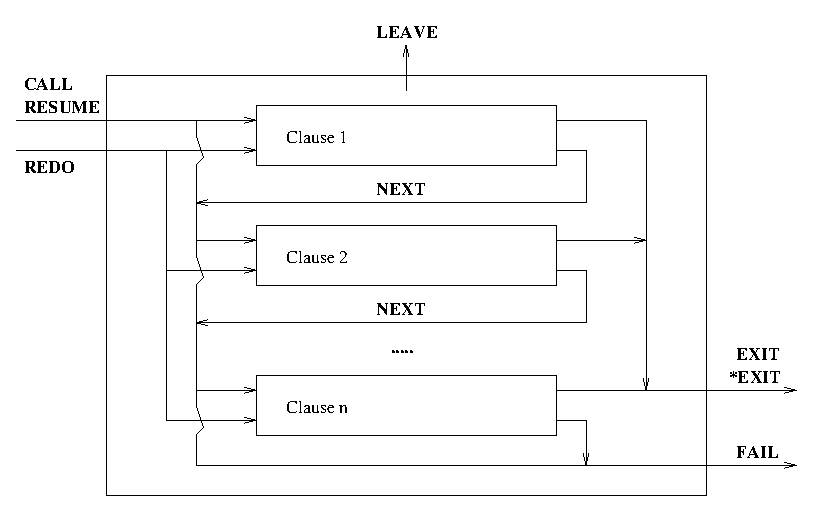
\includegraphics{boxmodel.eps}
\end{center}
\caption{The box model}
\end{figure}

Tracing the flow of the execution consists in tracing the crossing of
the execution flow through any of the port of the box.

The five basic ports of the box model of {\eclipse} are the CALL, EXIT,
REDO, FAIL and NEXT ports, the suspension facilities are traced through
the DELAY and RESUME ports, and the exceptional exit is indicated by LEAVE.

\begin{description}

\item[CALL:] When a procedure is invoked, the flow of the execution
enters the procedure box by its CALL port and enters the first clause
box which could (since not all clauses are tried, some of them being
sure to fail, i.e., indexing is shown) unify with the goal.
It may happen that a procedure is
called with arguments that make it sure to fail (because of
indexing). In such cases, the flow does not enter any clause box.

For each CALL port a new procedure box is created and is given:
\begin{itemize}
\item an \emph{invocation number} that is one higher than that given for
the most recent CALL port. This allows to uniquely identify a
procedure invocation and all its corresponding ports.

\item a \emph{level} that is one higher than that of its parent goal.
\end{itemize}

The displayed variable instantiations are the ones at call time,
i.e., before the head unification of any clause.

\item[EXIT:] When a clause of a predicate succeeds (i.e., unification
succeeded and all procedures called by the clause succeeded),
the flow gets out of the box by the EXIT port of both boxes (only
the EXIT port of the \emph{procedure box} is traced).

When a procedure exits non-deterministically (and there are still
other clauses to try on that procedure or one of its children goals
has alternatives which could be resatisfied), the EXIT port is traced
with an asterisk (*EXIT). When the last possibly matching clause of a
procedure is exited, the exit is traced without asterisk. This means
that this procedure box will never be retried as there is no other
untried alternative.

The instantiations shown in the EXIT port are the ones at exit time,
they result from the (successful) execution of the procedure.

\item[FAIL:] When a clause of a procedure fails (because head unification
failed or because a sub-goal failed), the flow of the execution exits
the clause box and leaves the procedure box via the FAIL port.
Note that the debugger cannot display any argument information at
FAIL ports (an ellipsis \verb:...: is displayed instead for each argument).

\item[NEXT:] If a clause fails and there is another possibly
matching clause to try, then that one is tried for unification.
The flow of the execution from the failure of one clause to the
head unification of a following clause is traced as a NEXT port.
The displayed variable instantiations are the same as those of the
corresponding CALL or REDO port.

\item[ELSE:]
This is similar to the NEXT port, but indicates that the next branch of a
\biptxtref{disjunction (;/2)}{;/2}{../bips/kernel/control/O-2.html}
it tried after the previous branch failed.
The predicate that gets displayed with the port is the predicate
which contains the disjunction (the immediate ancestor).

\item[REDO:] When a procedure box is exited trough an *EXIT port,
the box can be retried later to get a new solution. This will happen when a
later goal fails. The backtracking will cause failing of all
procedures that do not have any alternative, then the execution flow
will enter a
procedure box that an contains alternative through a REDO port.

Two situations may occur: either the last tried clause has called a
procedure that has left a choice point (it has exited through an
*EXIT port). In that case the nested procedure box is re-entered
though another REDO-port.

Otherwise, if the last clause tried does not contain any
nondeterministically exited boxes, but there are other untried clauses
in the procedure box, the next possibly matching clause will be tried.

The last REDO port in such a sequence is the one which contains the
actual alternative that is tried. The variable instantiations for all
REDO ports in such a sequence are the ones corresponding to the call
time of the last one.

%\item[UNIFY:] When a clause head successfully unifies with
%a called goal, a UNIFY port is traced to show the result of the
%unification. However, this port is not traced for unit clause since it
%is identical to the EXIT port.
%
%Please note that this port is not shown in the default settings but it
%can be switched on with the appropriate
%\bipref{set_leash/2}{../bips/kernel/debug/set_leash-2.html} call.

\item[LEAVE:]
This port allows to trace the execution of a the
\bipref{block/3}{../bips/kernel/control/block-3.html} and
\bipref{exit_block/1}{../bips/kernel/control/exit_block-1.html}
predicates within the box model.  The predicate
\bipref{block/3}{../bips/kernel/control/block-3.html} is traced as
a normal procedure.  If the goal in its first argument fails,
\bipref{block/3}{../bips/kernel/control/block-3.html} fails, if it
exits, \bipref{block/3}{../bips/kernel/control/block-3.html} exits.
If the predicate \bipref{exit_block/1}{../bips/kernel/control/exit_block-1.html}
is called (and exited since it
never fails), all the goals inside the matching block are left through
a special port called LEAVE, so that each entry port matches with an
exit port.  The recover procedure (in the third argument of
\bipref{block/3}{../bips/kernel/control/block-3.html}) is then
called and traced normally and
\bipref{block/3}{../bips/kernel/control/block-3.html} will exit or
fail (or even leave) depending on the recover procedure.

As with the FAIL port, no argument value are displayed in the LEAVE port.

%\item[CUT:] The cut is considered by the debugger as a predicate
%(it has its own box with a CALL and an EXIT port) that always
%succeeds.  The side effects it causes are traced through the CUT port.
%Each goal whose choice point is removed are traced with a CUT port.
%This port is actually not a real procedure port, it only notifies of
%the destruction (performed by the cut) of the choice point of a goal.
%When a goal has been cut, it can not be re-satisfied.  Therefore, the
%flow of the execution will never re-enter the procedure box through
%its REDO port. The displayed variable instantiations are the current
%ones.
%
%By default, the debugger only prints this port, but does not prompt for
%a command. This can be changed using
%\bipref{set_leash/2}{../bips/kernel/debug/set_leash-2.html}.
%
%\item[TRY:] The procedure creates a choicepoint. By default, the debugger does
%not show this port. Use
%\bipref{set_leash/2}{../bips/kernel/debug/set_leash-2.html} to make it
%visible.

\item[DELAY:]
The displayed goal becomes suspended. This is a singleton port, it does
not enter or leave a box. However, a new \emph{invocation number} is assigned
to the delayed goal, and this number will be used in the matching RESUME port.
The DELAY port is caused by one of the built-in predicates
\bipref{suspend/3}{../bips/kernel/suspensions/suspend-3.html},
\bipref{suspend/4}{../bips/kernel/suspensions/suspend-4.html},
\bipref{make_suspension/3}{../bips/kernel/suspensions/make_suspension-3.html}
or a delay clause.
The port is displayed just after the delayed goal has been created.

\item[RESUME:] When a waking condition causes the resuming of
a delayed goal, the procedure box is entered through its RESUME
port.  The box then behaves as if it had been entered through its CALL
port.  The invocation number is the same as in its previous DELAY port.
which makes it easy to identify corresponding delay and resume events.
However the depth level of the RESUME corresponds to the waking situation.
It is traced like a subgoal of the goal which has caused the waking.

\end{description}

In the rest of this chapter the user interface to the debugger is
described, including the commands available in the debugger itself as
well as built-in predicates which influence it.  Some of the debugger
commands are explained using an excerpt of a debugger session.  In
these examples, the user input is always underlined (it is in fact
not always output as typed) to distinguish it from the computer output.

\subsection{Breakpoints}

Breakpoints can be set on specific calls to a predicate, i.e., on a specific
body goal in the source, so that the
debugger will stop only at a CALL port only when that specific body goal is
executed. A breakpoint is specify by giving the source file and the line
number where the body goal is.

For example, if the following predicate is in a file called \notation{newtop},
with the following line numbers:

\begin{verbatim}
  243  check_words([],[]).
  244  check_words([Word|Words],[RevWord|RevWords]) :-
  245     check_words(Words,RevWords).
\end{verbatim}

The breakpoint for the body goal \notation{check_words(Words, RevWords)} would
be \notation{newtop:245}. Note that the file name must be sufficiently specified
for ECLiPSe to find the file from your current working directory.

For a call that has a breakpoint set, the execution will stop when the call
is made, i.e., at the CALL port for that specific body goal.

\section{Format of the Tracing Messages}
All trace messages are output to the
\notationidx{debug_output} stream.

The format of one trace line is as follows:
\begin{quote}
\begin{verbatim}
S+(4) 2 *EXIT<5> module:foo(one, X, two)   %>
12 3  4 5 6   7    8       9              10
\end{verbatim}
\end{quote}

\begin{enumerate}
\item The first character shows some properties of the
displayed procedure.
It may be one of
\begin{itemize}
\item C - an external procedure, not implemented in Prolog
\item S - a \emph{skipped} procedure, i.e., a procedure whose
subgoals are not traced
%\item N - a procedure compiled in non-debug mode, i.e., behaves like skipped.
\end{itemize}

\item A \notation{+} displayed here shows that the procedure has a spy point
  set,
  and a \notation{\#} shows that the specific call has a break-point set.
\index{spy point}

\item The number between parentheses shows the box invocation number
of this procedure call.  Since each box has a unique invocation
number, it can be used to identify ports that belong to the same box.
It also shows how many procedure redos have been made since the
beginning of the query.  Only boxes that can be traced obtain an
invocation number, for instance subgoals of a procedure which is
compiled in debug mode or has its skip-flag set are not numbered.

When a delayed goal is resumed, it keeps the invocation number it was
assigned when it delayed.  This makes it easy to follow all ports of a
specified call even in data-driven computation.

\item The second number shows the level or depth of the goal,
i.e., the number of its ancestor boxes.  When a subgoal is called, the
level increases and after exit it decreases again.  The initial level
is 1.

Since a resumed goal is considered to be a descendant of the procedure
that woke it, the level of a resumed goal may be different from
the level the goal had when it delayed.

\item An asterisk before an \notation{EXIT} means that this
procedure is nondeterministic and that it might be resatisfied.

\item The next word is the name of the port.
It might be missing if the displayed goal is not the current position
in the execution (e.g., when examining ancestors or delayed goals).

\begin{description}
\item[\notation{CALL}:] a procedure is called for the first time concerning a
  particular
invocation;

\item[\notation{DELAY}:] a procedure delays;

\item[\notation{EXIT}:] a procedure succeeds;

\item[\notation{FAIL}:] a procedure fails, there is no (other) solution;

\item[\notation{LEAVE}:] a procedure is left before having failed or exited
  because
of a call to \bipref{exit_block/1}{../bips/kernel/control/exit_block-1.html};

\item[\notation{NEXT}:] the next possibly matching clause of a procedure is
  tried
because unification failed or a sub-goal failed;

\item[\notation{ELSE}:] the next branch of a disjunction is tried because some
  goal
in the previous branch failed;

\item[\notation{REDO}:] a procedure that already gave a solution is called again
  for
an alternative;

\item[\notation{RESUME}:] a procedure is woken (the flow enters the procedure
  box as for
a call) because of a unification of a suspending variable.

%\item[UNIFY] unification succeeded (not shown for unit clauses).

\end{description}

\item This only appears if the goal is executing at a different priority
  than 12, the normal priority. The number between the angled brackets
  shows the priority (between 1 and 11) that the  goal is executed at.

\item For the tty debugger, the optional module name followed by a colon.
Printing of the module can be enabled and disabled by the debugger
command \notation{m}.\dbgcmdidx{m}{module}
If it is enabled, the module from where the procedure is called is
displayed.  By default the module printing is disabled. With tkeclipse, the
module name is not displayed with the traceline, instead, you can get the
information by right holding the mouse button over the trace line in the
call stack window.

\item The goal is printed according to the current instantiations
of its variables.  Arguments of the form \notation{...} represent subterms
that are not printed due to the depth limit in effect.
The depth limit can be changed using the
\notation{<}\dbgcmdidxPlus{$<$}{<}{print depth} command.

The goal is printed with the current \notation{output_mode} settings.
which can be changed using the
\notation{o}\dbgcmdidx{o}{output mode} command.

\item The prompt of the debugger, which means that it is waiting
for a command from the user. Note there is no prompt when tkeclipse tracer
is used.
\end{enumerate}

\section{Debugging-related Predicate Properties}

Predicates have a number of properties which can be listed using the
\bipref{pred/1}{../bips/kernel/env/pred-1.html} built-in.
The following predicate flags and properties affect the way the
predicate is traced by the debugger:
\begin{quote}
\begin{description}
\item[debugged]\mbox{}\\
        Indicates whether the predicate has been compiled in debug-compile mode.
        If \notation{on}, calls to the predicate's subgoal will be traced.
        The value of this property can only be changed by re-compiling
        the predicate in a different mode.

\item[leash]\mbox{}\\
        If \notation{notrace}, no port of the predicate will be shown
        in the trace (but the invocations will be counted nevertheless).
        If \notation{stop}, the ports of this predicate will be shown and
        the debugger will stop and await new commands.
        (The \notation{print} setting is currently not supported).
        The value of this property can be changed with
        \bipref{traceable/1}{../bips/kernel/debug/traceable-1.html},
        \bipref{untraceable/1}{../bips/kernel/debug/untraceable-1.html} or
        \bipref{set_flag/3}{../bips/kernel/compiler/set_flag-3.html}.

\item[spy]\mbox{}\\
        If \notation{on}, the predicate has a spy-point and the debugger will
        stop at its ports when in leap mode.
        The value of this property can be changed with
        \bipref{spy/1}{../bips/kernel/debug/spy-1.html},
        \bipref{nospy/1}{../bips/kernel/debug/nospy-1.html} or
        \bipref{set_flag/3}{../bips/kernel/compiler/set_flag-3.html}.

\item[skipped]\mbox{}\\
        If \notation{on}, the predicate's subgoal will not be traced even
        if it has been compiled in debug-compile mode.
        The value of this property can be changed with
        \bipref{skipped/1}{../bips/kernel/debug/skipped-1.html},
        \bipref{unskipped/1}{../bips/kernel/debug/unskipped-1.html} or
        \bipref{set_flag/3}{../bips/kernel/compiler/set_flag-3.html}.

\item[start_tracing]\mbox{}\\
        If \notation{on}, a call to the predicate will activate the debugger if
        it
        is not already running.
        Only the execution within this predicate's box will be traced.
        This is useful for debugging part of a big
        program without having to change the source code.
        The effect is similar to wrapping all call of the predicate into
        \bipref{trace/1}{../bips/kernel/debug/trace-1.html}.
\end{description}
\end{quote}


%{\it Leashing} stands for the way the trace lines of a
%procedure at a port are displayed and handled by the debugger.
%There are three distinct leash levels:
%
%\begin{description}
%\item[stop] Full leashing, the trace line is displayed, the debugger prints
%a prompt and waits for a command from the user.
%
%\item[print] The trace line is only displayed and the debugger
%does not stop but it continues to the next trace line.
%
%\item[notrace] The trace line is not displayed and
%the debugger does not prompt for a command.
%\end{description}
%The leashing mode can be specified separately for ports and procedures.
%The debugger command {\bf p} and
%\index{p --- port leashing (debugger cmd)}
%the predicate \bipref{set_leash/2}{../bips/kernel/debug/set_leash-2.html}
%are for ports, e.g.,
%\begin{quote}\begin{verbatim}
%set_leash(next, notrace).
%\end{verbatim}\end{quote}
%will suppress printing of all NEXT ports.
%To change the leash mode for a certain procedure,
%the predicate \bipref{set_flag/3}{../bips/kernel/compiler/set_flag-3.html} or
%the debugger command {\bf t}
%\index{t --- procedure trace mode (debugger cmd)}
%are used. For instance
%\begin{quote}\begin{verbatim}
%set_flag(p/3, leash, print).
%\end{verbatim}\end{quote}
%will cause all ports of the procedure p/3 to be printed, but the
%debugger will not stop or prompt for commands.
%For each trace line, the
%effective leash mode is combined from the mode of the current
%procedure and the current port and if the two are not equal, the more
%restrictive one is taken.
%
%A particularly useful combination is to set a spy point on a procedure
%\index{spy point}
%and set its leash mode to {\tt print}. This will cause the
%debugger to print a continuous trace of all ports involving this procedure.


\section{Starting the Debugger}

Several methods can be used to switch the debugger on.
If the textual interactive top-level is used, the commands
\bipref{trace/0}{../bips/kernel/debug/trace-0.html} and
\bipref{debug/0}{../bips/kernel/debug/debug-0.html} are used to
switch the debugger on for the following queries typed from the
top-level.
\bipref{trace/0}{../bips/kernel/debug/trace-0.html} will switch the
debugger to \notation{creep} mode whereas
\bipref{debug/0}{../bips/kernel/debug/debug-0.html} will switch it
in leap mode.

For the \tkeclipse{} graphical toplevel, the debugger may be switched on by
starting the tracer from the Tools menu before executing the query. This
puts the debugger in \notation{creep} mode.

When the debugger is in \notation{creep} mode, it will
prompt for a command at the crossing of the first
%leashed
port of a
leashed procedure.  When the debugger is in leap mode,
it will prompt for a command at the first port of a leashed
procedure that has a spy point.  The debugger is switched off either
from the toplevel with the commands
\bipref{nodebug/0}{../bips/kernel/debug/nodebug-0.html} or
\bipref{notrace/0}{../bips/kernel/debug/notrace-0.html}, or by
typing \notation{n} or \notation{N} to the debugger prompt.

A spy point can be set on a procedure, or a breakpoint on a specific call,
using
\bipref{spy/1}{../bips/kernel/debug/spy-1.html} (which will
\index{spy point} also switch the debugger to leap)
and removed
with \bipref{nospy/1}{../bips/kernel/debug/nospy-1.html}.  They
both accept a \about{SpecList} as argument.  Note that
\bipref{set_flag/3}{../bips/kernel/compiler/set_flag-3.html} can
be used to set and reset spy points without switching the debugger on
and without printing messages.

\bipref{debugging/0}{../bips/kernel/debug/debugging-0.html} can be
used to list the spied predicates and the current debugger mode.

\begin{quote}
\begin{verbatim}
[eclipse 1]: spy writeln/1.
spypoint added to writeln / 1.

yes.
Debugger switched on - leap mode
[eclipse 2]: debugging.
Debug mode is leap
writeln / 1 is being spied

yes.
[eclipse 3]: true, writeln(hello), true.
B+(2) 0  CALL   writeln(hello) %> l leap
hello
B+(2) 0  EXIT   writeln(hello) %> c creep
B (3) 0  CALL   true %> l leap

yes.
[eclipse 4]: trace.
Debugger switched to creep mode

yes.
[eclipse 5]: true, writeln(hello), true.
B (1) 0  CALL   true %> c creep
B (1) 0  EXIT   true %> c creep
B+(2) 0  CALL   writeln(hello) %> l leap
hello
B+(2) 0  EXIT   writeln(hello) %> l leap

yes.
\end{verbatim}
\end{quote}

\section{Debugging Parts of Programs}

\subsection{Mixing debuggable and non-debuggable code}

The debugger can trace only procedures which have been compiled in
debug mode.  The compiler debug mode is by default switched on and it
can be changed globally by setting the flag \notation{debug_compile} with the
\bipref{set_flag/2}{../bips/kernel/env/set_flag-2.html}
predicate or using
\bipref{dbgcomp/0}{../bips/kernel/obsolete/dbgcomp-0.html} or
\bipref{nodbgcomp/0}{../bips/kernel/obsolete/nodbgcomp-0.html}.
The global compiler debug mode can be overruled on a file-by-file basis
using one of the compiler pragmas
\begin{quote}
\begin{verbatim}
:- pragma(nodebug).
:- pragma(debug).
\end{verbatim}
\end{quote}
Once a program (or a part of it) has been
debugged, it can be compiled in \notation{nodbgcomp} mode so that all
optimisations are done by the compiler.  The advantages of
non-debugged procedures are

\begin{itemize}
\item They run slightly faster than the debugged procedures
when the debugger is switched off.  When the debugger is switched on,
the non-debugged procedures run considerably faster than the debugged
ones and so the user can selectively influence the speed of the code
which is being traced as well as its space consumption.

\item Their code is shorter than that of the debugged procedures.
\end{itemize}

Although only procedures compiled in the \notation{dbgcomp} mode can be
traced, it is possible to mix the execution of procedures in both
modes.  Then, calls of \notation{nodbgcomp} procedures from \notation{dbgcomp}
ones are
traced, however further execution within \notation{nodbgcomp} procedures,
i.e., the execution of their subgoals, no matter in which mode, is not
traced.  In particular, when a \notation{nodbgcomp} procedure calls a
\notation{dbgcomp}
one, the latter is normally not traced.
There are two important exceptions from this rule:
\begin{itemize}
\indextt{waking/1}
\item When a debuggable procedure has delayed and its DELAY port has
been traced, then its RESUME port is also traced, even when it is woken
inside non-debuggable code.
\index{\atsym/2@\notation{"@/2}}
\indextt{subcall/2}
\item When non-debuggable code \emph{meta-calls} a debuggable procedure
(i.e., via \bipref{call/1}{../bips/kernel/control/call-1.html}),
then this procedure can be traced.  This is a useful feature for the
implementation of meta- predicates like
\bipref{setof/3}{../bips/kernel/allsols/setof-3.html}, because it
allows to hide the details of the setof-implementation, while allowing
to trace the argument goal.
\end{itemize}

Setting a procedure to skipped (with
\bipref{set_flag/3}{../bips/kernel/compiler/set_flag-3.html} or
\bipref{skipped/1}{../bips/kernel/debug/skipped-1.html}
)
%or using the fast skip command of the debugger (\notation{F}) are also ways
is another way
to speed up the execution of procedures that need not be
debugged.  The debugger will ignore everything that is called inside
the skipped procedure like for a procedure compiled in \notation{nodbgcomp}
mode.  However, the debugger will keep track of the execution of a
procedure skipped with the command \notation{s} of the debugger so that it
will be possible to ``creep'' in it on later backtracking or switch the
debugger to \notation{creep} mode while the skip is running (e.g.,  by
interrupting a looping predicate with \notation{\^{}C} and switching to
\notation{creep} mode).

The two predicates
\bipref{trace/1}{../bips/kernel/debug/trace-1.html} and
\bipref{debug/1}{../bips/kernel/debug/debug-1.html} can be used to
switch on the debugger in the middle of a program.  They execute their
argument in \notation{creep} or \notation{leap} mode respectively.  This is
particularly useful when debugging large programs that take too much
time (or need a lot of memory) to run completely with the debugger.
\begin{quote}
\begin{verbatim}
[eclipse 1]: debugging.
Debugger is switched off

yes.
[eclipse 2]: big_goal1, trace(buggy_goal), big_goal2.
Start debugging - creep mode
  (1) 0  CALL   buggy_goal %> c creep
  (1) 0  EXIT   buggy_goal %> c creep
Stop debugging.

yes.
\end{verbatim}
\end{quote}

It is also possible to enable the debugger in the middle of execution
without changing the code.  To do so, use
\bipref{set_flag/3}{../bips/kernel/compiler/set_flag-3.html}
to set the \notationidx{start_tracing} flag of the predicate of interest.
Tracing will then start (in leap mode) at every call of this
predicate.\footnote{%
  Provided the call has been compiled in debug_compile mode,
  or the call is a meta-call.}
To see the starting predicate itself,
set a spy point in addition to the \notation{start_tracing} flag:
\begin{quote}
\begin{verbatim}
[eclipse 1]: debugging.
Debugger is switched off

yes.
[eclipse 2]: set_flag(buggy_goal/0, start_tracing, on),
             set_flag(buggy_goal/0, spy, on).

yes.
[eclipse 3]: big_goal1, buggy_goal, big_goal2.
 +(0) 0 CALL  buggy_goal   %> creep
 +(0) 0 EXIT  buggy_goal   %> creep

yes.
\end{verbatim}
\end{quote}

In tkeclipse, the debugger can also be started in this way. The tracer tool
will popup at the appropriate predicate if it has not been invoked
already. The \notation{start_tracing} flag can also be set with the predicate
browser tool.

%----------------------------------------------------------------------
\section{Using the Debugger via the Command Line Interface}
%----------------------------------------------------------------------
This section describe the commands available at the debugger prompt
in the debugger's command line interface (for the graphical user
interface, please refer to the online documentation).

Commands are entered by typing the corresponding key
(without newline), the case of the letters is significant.  The action
of some of them is immediate, others require additional parameters to
be typed afterwards.  Since the {\eclipse} debugger has the possibility to
display not only the goal that is currently being executed (the {\it
current} goal or procedure), but also its ancestors, some of the
commands may work on the \emph{displayed} procedure whatever it is, and
others on the \emph{current} one.
% Any undefined debugger command will reset the displayed procedure to the
% current one.

\subsection{Counters and Command Arguments}
Some debugger commands accept a counter (a small integer number)
before the command letter (e.g., \notation{c}, i.e., \notation{creep}).
The number is just prefixed to the command and terminated by the
command letter itself. If a counter is given for a command that
doesn't accept a counter, it is ignored.

When a counter is used and is valid for the command,
the command is repeated, decrementing the counter until zero.
When repeating the command, the command and the remaining counter
value is printed after the debugger prompt instead of waiting for user input.

Some commands prompt for a parameter, e.g., the \notation{j} (\notation{jump)}
command asks for the number of the level to which to jump.
Usually the parameter has a sensible default value (which is printed
in square backets). If just a newline is typed, then the default value
is taken. If a valid parameter value is typed, followed by newline,
this value is taken. If an illegal letter is typed, the command is aborted.


%----------------------------------------------------------------------
\subsection{Commands to Continue Execution}
%----------------------------------------------------------------------
All commands in this section continue program execution.
They difference between them is the condition under which execution
will stop the next time.  When execution stops again, the next trace
line is printed and a new command is accepted.

\begin{descr}{1cm}

\ncmd{c}{creep}\\
This command allows exhaustive tracing: the execution stops at the
next port of any leashed procedure.  No further parameters are
required, a counter \about{n} will repeat the command \about{n} times.
It always applies on the current procedure, even when the displayed
procedure is not the current one (e.g., during term inspection).
An alias for the \notation{c} command is to just type newline (Return-key).

\ncmd{s}{skip}\\
If given at an entry port of a box (CALL, RESUME, REDO), this command skips
the execution until an exit port of this box (EXIT, FAIL, LEAVE).
If given in an exit port it works like \notation{creep}.
(Note that sometimes the \notation{i} command is more appropriate, since it
skips to the next port of the current box, no matter which).
A counter, if specified, repeats this command.

%\ncmd{F}{fast skip}\\
%Is similar to the skip command \notation{s}. The difference is that the
%debugger does not keep track of the execution during the skip so that
%it is faster. As a result, it is not possible to {\it creep} later on
%inside this procedure (e.g., it will not be possible to 'creep'
%through this procedure on later backtracking, and switching the debugger
%back to {\it creep} mode using \^\space C while the skipped procedure is
%looping will have no effect).

\ncmd{l}{leap}\\
Continues to the next spy point (any port of a procedure
which has its spy flag set).
\index{spy point}
A counter, if specified, repeats this command.

\mcmd{i}{invocation skip}\\
Continue to the next port of the box with the invocation number
specified. The default invocation number is the one of the current box.
Common uses for this command are to skip from CALL to NEXT, from NEXT
to NEXT/EXIT/FAIL, from *EXIT to REDO, or from DELAY to RESUME.

\mcmd{j}{jump to level}\\
Continue to the next port with the specified nesting level (which can
be higher or lower than the current one).
The default is the parent's level, i.e., to continue until the current
box is exited, ignoring all the remaining subgoals of the current clause.
This is particularly useful when a \notation{c} (\notation{creep}) has been
typed where a \notation{s} (\notation{skip}) was wanted.

\cmd{n}{nodebug}\\
This command switches tracing off for the remainder of the execution.
However, the next top-level query will be traced again.
Use \notation{N} to switch tracing off permanently.

\cmd{q}{query the failure culprit}\\
The purpose of this command is to find out why a goal has failed (FAIL)
or was aborted with an exit_block (LEAVE).  It prints the invocation
number of the goal which caused the failure.  You can then re-run the
program in \notation{creep} mode and type \notation{q} at the first command
  prompt.  This will
then offer you to jump to the CALL port of the culprit goal.
%cannot quote: too wide
\begin{verbatim}
[eclipse 3]: p.
  (1) 1 CALL  p   %> skip
  (1) 1 FAIL  p   %> query culprit
failure culprit was (3) - rerun and type q to jump there   %> nodebug? [y]
No (0.00s cpu)

[eclipse 4]: p.
  (1) 1 CALL  p   %> query culprit
failure culprit was (3) - jump to invoc: [3]?
  (3) 3 CALL  r(1)   %> creep
  (3) 3 FAIL  r(...)   %> creep
  (2) 2 FAIL  q   %> creep
  (1) 1 FAIL  p   %> creep
No (0.01s cpu)
\end{verbatim}

\cmd{v}{var/term modification skip}\\
This command sets up a monitor on the currently displayed term,
which will cause a MODIFY-port to be raised on each modification to
any variable in the term. These ports will all have a unique invocation
number which is assigned and printed at the time the command is issued.
This number can then be used with the \notation{i} command to skip to where
the modifications happen.
%cannot quote: too wide
\begin{verbatim}
[eclipse 4]: [X, Y] :: 1..9, X #>= Y, Y#>1.
  (1) 1 CALL  [X, Y] :: 1..9   %> var/term spy? [y]
Var/term spy set up with invocation number (2)   %> jump to invoc: [1]? 2
  (2) 3 MODIFY  [X{[1..9]}, Y{[2..9]}] :: 1..9   %> jump to invoc: [2]?
  (2) 4 MODIFY  [X{[2..9]}, Y{[2..9]}] :: 1..9   %> jump to invoc: [2]?
\end{verbatim}
Note that these monitors can also be set
up from within the program code using one of the built-ins
\bipref{spy_var/1}{../bips/kernel/debug/spy_var-1.html} or
\bipref{spy_term/2}{../bips/kernel/debug/spy_term-2.html}.

%\cmd{v}{variable skip}\\
%This command allows to resume tracing when a specified variable
%becomes instantiated.  The debugger prompts for the name of the
%variable whose instantiation is looked for.  The variable identification is
%either its name or, in case it is not unique, its number.
%The variable number has the format
%{\it _cnnn} where {\it c} is {\it l}, denoting a local
%variable, or empty, denoting a global variable.
%If variables are displayed without their numbers,
%use the {\bf o} command to toggle the 'V' flag which displays the numbers
%in the form {\bf Name_c123} and then type in the
%{\bf _c123} to identify the variable number.
%
%If the specified variable is already instantiated, or if the
%variable is not accessible from the debugger (e.g., the life time of
%the variable is already expired or the variable has never been traced
%by the debugger) a warning is printed.  Otherwise, the execution is
%continued without tracing until the variable is instantiated, i.e.,
%bound to a constant or a compound term.  Then the debugger displays
%its current value and resumes tracing.  The tracing is resumed at the
%UNIFY port of a rule or at the EXIT port of a unit clause, depending
%on the type of the clause whose head unification has bound the
%specified variable.  The UNIFY port is displayed even if it is set to
%{\it not traced}, to allow a precise location of the call that has
%instantiated the variable.
%
%\begin{quote}\begin{alltt}
%  (5) 1  CALL   conslist(3, X) (dbg)?- v
%Variable to be bound (Name or _[lg]NNN): _X\(<NL>\)
%Variable has been bound to [3|L] in
%  (5) 1  UNIFY  conslist(3, [3|L]) (dbg)?-
%\end{alltt}\end{quote}
%
%It may happen that the lifetime of the variable expires before it is
%bound. In this case the debugger prints a message and traces the next
%port normally.
%
%\begin{quote}\begin{verbatim}
%  (1) 0  CALL   p (dbg)?- o
%current output mode is "QPm", toggle chars: v
%new mode is "QvPm"
%  (1) 0  CALL   p (dbg)?- c creep
%  (2) 1  CALL   p(_1122) (dbg)?- V
%Variable to be bound (Name or _[lg]NNN):  _1122
%  (2) 1  EXIT   p(_1122)
%C (3) 1  CALL   fail
%C (3) 1  FAIL   fail
%  (1) 0  NEXT   p
%Variable will never be bound
%  (1) 0  EXIT   p (dbg)?-
%\end{verbatim}\end{quote}

%\ncmd{w}{wake skip}\\
%This command is used only for delayed goals.  When it is used at the
%DELAY port, it skips the execution until this goal is resumed.  This
%command does not accept any arguments.  Since the resumed goal has
%the same invocation number like the delayed one, the {\bf j} or {\bf
%i} commands could be used for the same purpose,
%\index{j --- jump (debugger cmd)}
%\index{i --- invocation skip (debugger cmd)}
%however the {\bf w} command has an additional feature, namely that the
%tracing is also resumed when the delayed goal disappears because the
%system backtracked to a state before this goal was called and delayed.
%A specified counter is ignored.  The command is executed even if the
%displayed procedure is not the current one, as long as the displayed
%port is DELAY.  On other ports an error message is printed.
%
% \begin{quote}\begin{verbatim}
% [eclipse 1]: spy a/1.
% spypoint added to a / 1.
%
% yes.
% Debugger switched on - leap mode
% [eclipse 2]: p.
%  +(6) 1  CALL   a(_39) (dbg)?- d delayed goals
%
% Delayed goals:
%   (3) p(_41, _39)
%
%  +(6) 1  CALL   a(_39) (dbg)?- u use goal (3)
%   (3) 1  DELAY  p(_41, _39) (dbg)?- W wake
%  +(6) 1  EXIT   a(1)
%   (7) 1  CALL   b(1)
%   (7) 1 *EXIT   b(1)
%   (8) 1  CALL   c(1)
%   (8) 1 *EXIT   c(1)
%  +(9) 1  CALL   a(_41)
%   (3) 2  RESUME p(1, 1) (dbg)?-
% \end{verbatim}\end{quote}

\mcmd{z}{zap}\\
This command allows to skip over, or to a specified port.  When this
command is executed, the debugger prompts for a port name (e.g.,
\notation{fail})
or a negated port name (e.g., \tld\notation{exit}).
Execution then continues until the specified port appears or,
in the negated case, until a port other than the specified one appears.
The default is the negation of the current port, which is useful
when exiting from a deep recursion (a long sequence of EXIT or FAIL ports).

%\ncmd{e}{error search}\\
%This is a predefined macro; it is set to {\tt "zleave"} i.e., zap to a LEAVE
%port. It is useful for example to skip until an error that calls {\bf
%exit_block/1} occurs.

\end{descr}

%----------------------------------------------------------------------
\subsection{Commands to Modify Execution}
%----------------------------------------------------------------------
\begin{descr}{1cm}

\mcmd{f}{fail}\\
Force a failure of the procedure with the specified invocation number.
The default is to force failure of the current procedure.

\cmd{a}{abort}\\
Abort the execution of the current query and return to the top-level.
The command prompts for confirmation.
\end{descr}


%----------------------------------------------------------------------
\subsection{Display Commands}
%----------------------------------------------------------------------
This group of commands cause some useful information to be displayed.

\begin{descr}{1cm}

\mcmd{d}{delayed goals}\\
Display the currently delayed goals. The optional argument allows
to restrict the display to goal of a certain priority only.
The goals are displayed in a format similar to the trace lines,
except that there is no depth level and no port name.
Instead, the goal priority is displayed in angular brackets:
\begin{quote}
\begin{verbatim}
[eclipse 5]: [X, Y] :: 1..9, X #>= Y, Y #>= X.
  (1) 1 CALL  [X, Y] :: 1..9   %> creep
  (1) 1 EXIT  [X{[1..9]}, Y{[1..9]}] :: 1..9   %> creep
  (2) 1 CALL  X{[1..9]} - Y{[1..9]}#>=0   %> creep
  (3) 2 DELAY  X{[1..9]} - Y{[1..9]}#>=0   %> creep
  (2) 1 EXIT  X{[1..9]} - Y{[1..9]}#>=0   %> creep
  (4) 1 CALL  Y{[1..9]} - X{[1..9]}#>=0   %> creep
  (5) 2 DELAY  Y{[1..9]} - X{[1..9]}#>=0   %> delayed goals
                                                with prio: [all]?
------- delayed goals -------
  (3) <2>  X{[1..9]} - Y{[1..9]}#>=0
  (5) <2>  Y{[1..9]} - X{[1..9]}#>=0
------------ end ------------
  (5) 2 DELAY  Y{[1..9]} - X{[1..9]}#>=0   %>
\end{verbatim}
\end{quote}

\mcmd{u}{scheduled goals}\\
Similar to the \notation{d} command, but displays only those delayed goals
that are already scheduled for execution.
The optional argument allows
to restrict the display to goal of a certain priority only. Example:
\begin{quote}
\begin{verbatim}
[eclipse 13]: [X,Y,Z]::1..9, X#>Z, Y#>Z, Z#>1.
  (1) 1 CALL  [X, Y, Z] :: 1..9   %> creep
  (1) 1 EXIT  [X{[1..9]}, Y{[1..9]}, Z{[1..9]}] :: 1..9   %> creep
  (2) 1 CALL  X{[1..9]} - Z{[1..9]}+-1#>=0   %> creep
  (3) 2 DELAY  X{[2..9]} - Z{[1..8]}#>=1   %> creep
  (2) 1 EXIT  X{[2..9]} - Z{[1..8]}+-1#>=0   %> creep
  (4) 1 CALL  Y{[1..9]} - Z{[1..8]}+-1#>=0   %> creep
  (5) 2 DELAY  Y{[2..9]} - Z{[1..8]}#>=1   %> creep
  (4) 1 EXIT  Y{[2..9]} - Z{[1..8]}+-1#>=0   %> creep
  (6) 1 CALL  0 + Z{[1..8]}+-2#>=0   %> creep
  (3) 2 RESUME  X{[2..9]} - Z{[2..8]}#>=1   %> scheduled goals
                                                with prio: [all]?
------ scheduled goals ------
  (5) <2>  Y{[2..9]} - Z{[2..8]}#>=1
------------ end ------------
  (3) 2 RESUME  X{[2..9]} - Z{[2..8]}#>=1   %>
\end{verbatim}
\end{quote}

%\cmd{\accent 94}{delayed by a variable}\\
%This command displays goals suspended by a specified
%variable, i.e., like with the built-in predicate {\bf delayed_goals/2}.
%The debugger will prompt for a variable number like in the {\bf v}
%command and then print the delayed goals similarly to the {\bf d}
%command.

\cmd{G}{all ancestors}\\
Prints all the current goal's ancestors from the oldest to the newest.
The display format is similar to trace lines,
except that {\tt ....} is displayed in the port field.

\cmd{.}{print definition}\\
If given at a trace line, the command displays the source code of the
current predicate.
If the predicate is not written in Prolog, or has not been compiled from
a file, or the source file is inaccessible, no information can be displayed.

\cmd{w}{write source context for current goal}\\
Lists the source lines around the current goal displayed by the trace line,
showing the context of the goal. For example:

\begin{quote}
\begin{verbatim}
  (230) 4 CALL  check_word(what, _5824)   %> write source lines
Source file: /homes/user/EclipseTests/Chatq/newtop
  241  :- mode check_words(+,-).
  242
  243  check_words([],[]).
  244  check_words([Word|Words],[RevWord|RevWords]) :-
  245>    check_word(Word,RevWord),
  245     check_words(Words,RevWords).
  246
  247  :- mode check_word(+,-).
  248
   %>
\end{verbatim}
\end{quote}

The listing shows the line numbers for the source lines, with a \notation{>}
marking the line with the current goal. Note it is the actual body goal
that is shown, rather than the predicate definition as in the \notation{.}
command.
An optional numeric argument can be given before the command, specifying
the number of lines surrounding (i.e., before and after) the current goal
that should be listed:

\begin{quote}
\begin{verbatim}
    %> 2write source lines
Source file: /homes/user/EclipseTests/Chatq/newtop
  243  check_words([],[]).
  244  check_words([Word|Words],[RevWord|RevWords]) :-
  245>    check_word(Word,RevWord),
  245     check_words(Words,RevWords).
  246
   %>
\end{verbatim}
\end{quote}

Source is only shown if the source information is available---that is,
the code has to be compiled debuggable from a file, and not all goals have
source information; for example, goals in meta-calls (e.g., those inside a
\predspec{block/3}). Also, source context cannot be shown at a RESUME port.

\cmd{h}{help}\\
Print a summary of the debugger commands.

\cmd{\query}{help}\\
Identical to the \notation{h} command.

\end{descr}


%----------------------------------------------------------------------
\subsection{Navigating among Goals}
%----------------------------------------------------------------------

While the debugger waits for commands, program execution is always
stopped at some port of some predicate invocation box, or goal.
Apart from this current goal, two types of other goals are also active.
These are the ancestors of the current goal (the enclosing, not yet
exited boxes in the box model) and the delayed goals.
The debugger allows to navigate among these goals and inspect them.

\begin{descr}{1cm}

\cmd{g}{ancestor}\\
Move to and display the ancestor goal (or parent) of the displayed goal.
Repeated application of this command allows to go up the call stack.

\mcmd{x}{examine goal}\\
Move to and display the goal with the specified invocation number.
This must be one of the active goals, i.e., either an ancestor of the
current goal or one of the currently delayed goals.
The default is to return to the current goal, i.e., to the goal at
whose port the execution is currently stopped.
\end{descr}

%----------------------------------------------------------------------
\subsection{Inspecting Goals and Data}
%----------------------------------------------------------------------

This family of commands allow the subterms in the goal displayed at the
port to be inspected.
\index{inspect subterm commands (debugger)}
The ability to inspect subterms is designed to help overcome two problems
when examining a large goal with the normal display of the goal at a debug
port:
\begin{enumerate}
\item Some of the subterms may be omitted from the printed goal because
of the print-depth;

\item If the user is interested in particular subterms, it
may be difficult to precisely locate them from the surrounding arguments,
even if it is printed.
\end{enumerate}

With inspect subterm commands, the user is able to issue commands to
navigate through the subterms of the current goal and examine them.
A \emph{current subterm} of the goal is maintained, and this is
printed after each inspect subterm command, instead of the entire goal.
Initially, the current subterm is set to the goal, but this can then be
moved to the subterms of the goal with navigation commands.

Once inspect subterm is initiated by an inspect subterm command, the
debugger enters into the inspect subterm mode. This is indicated in the
trace line by \notation{INSPECT} instead of the name of the port, and in
addition,
the goal is not shown on the trace line:

\begin{quote}
\begin{verbatim}
        INSPECT  (length/2)   %>
\end{verbatim}
\end{quote}

Instead of showing the goal, a summary of the current subterm---generally its
functor and arity if the subterm is a structure---is shown in brackets.

\begin{descr}{1cm}


\mcmd{ \#}{move down to {\it par}th argument}\\
The most basic command of inspect subterm is to move the current subterm to
an argument of the existing current subterm. This is done by typing a
number followed by carriage return, or by typing  \verb:#:, which causes the
debugger to prompt for a number. In both cases, the number specifies the
argument number to move down to.
In the following example, the \verb:#: style of the command is used to move
to the first argument, and the number style of the command to move to the
third argument:

\begin{quote}
\begin{verbatim}
  (1) 1 CALL  foo(a, g(b, [1, 2]), X)   %> inspect arg #: 1<NL>
a
        INSPECT  (atom)   %>
\end{verbatim}
\end{quote}

\begin{quote}
\begin{verbatim}
  (1) 1 CALL  foo(a, g(b, [1, 2]), X)   %>  3<NL>
X
        INSPECT  (var)   %>
\end{verbatim}
\end{quote}

The new current subterm is printed, followed by the INSPECT
trace line. Notice that the summary shows the type of the current
subterm, instead of \pattern{Name/Arity}, since in both cases the subterms are
not structures.

If the current subterm itself is a compound term, then it is possible to
recursively navigate into the subterm:

\begin{quote}
\begin{verbatim}
  (1) 1 CALL  foo(a, g(b, [1, 2]), X)   %> 2<NL>
g(b, [1, 2])
        INSPECT  (g/2)   %> 2<NL>
[1, 2]
        INSPECT  (list  1-head 2-tail)   %> 2<NL>
[2]
        INSPECT  (list  1-head 2-tail)   %>
\end{verbatim}
\end{quote}

Notice that lists are treated as a structure with arity 2, although the
functor (\predspec{./2}) is not printed.

In addition to compound terms, it is also possible to navigate into the
attributes of attributed variables:

\begin{quote}
\begin{verbatim}
[eclipse 21]: suspend(foo(X), 3, X->inst), foo(X).<NL>
  (1) 1 DELAY  foo(X)   %> <NL>
creep
  (2) 1 CALL  foo(X)   %> 1<NL>
X
        INSPECT  (attributes  1-suspend 2-fd )   %>1<NL>
suspend(['SUSP-1-susp'|_218] - _218, [], [])
        INSPECT  (struct suspend/3)   %>
\end{verbatim}
\end{quote}

The variable X is an attributed variable in this case, and when it is the
current subterm, this is indicated in the trace line. The debugger also
shows the user the currently available attributes, and the user can then
select one to navigate into (\notation{fd} is available in
this case because the finite domain library was loaded earlier in the
session. Otherwise, it would not be available as a choice here).

Note that the \predspec{suspend/3} summary contains a \notation{struct} before
it. This is because the \predspec{suspend/3} is a predefined structure with
field names (see section~\ref{chapstruct}). It is possible to view the
field names of such structures using the \notation{.} command in inspect mode.

If the number specified is larger than the number of the arguments of the
current subterm, then an error is reported and no movement is made:

\begin{quote}
\begin{verbatim}
foo(a, g(b, [1, 2]), 3)
        INSPECT  (foo/3)   %> 4<NL>

Out of range.....

foo(a, g(b, [1, 2]), 3)
        INSPECT  (foo/3)   %>
\end{verbatim}
\end{quote}

\ncmd{uparrow key}{move current subterm up by \about{n} levels}
\ncmd{A}{move current subterm up by \about{n} levels}\\
In addition to moving the current subterm down, it can also be moved up
from its current position. This is done by typing the uparrow key. This key
is mapped to \notation{A} by the debugger, so one can also type
\notation{A}. Typing \notation{A} may be necessary for some configurations
(combination of keyboards and operating systems) because the uparrow key is
not correctly mapped to \notation{A}.

An optional argument can preceded the uparrow keystroke, which indicates
the number of levels to move up. The default is 1:

\begin{quote}
\begin{verbatim}
  (1) 1 CALL  foo(a, g(b, [1, 2]), 3)   %> 2<NL>
g(b, [1, 2])
        INSPECT  (g/2)   %> 1<NL>
b
        INSPECT  (atom)   %> up subterm
g(b, [1, 2])
        INSPECT  (g/2)   %> 1up subterm
foo(a, g(b, [1, 2]), 3)
        INSPECT  (foo/3)   %>
\end{verbatim}
\end{quote}

The debugger prints \notation{up subterm} when the uparrow key is typed. The
current subterm moves back up the structure to its parent for each level it
moves up, and the above move can be done directly by specifying 2 as the
levels to move up:

\begin{quote}
\begin{verbatim}
b
        INSPECT  (atom)   %> 2up subterm
foo(a, g(b, [1, 2]), 3)
        INSPECT  (foo/3)   %>
\end{verbatim}
\end{quote}

If the number of levels specified is more than the number of levels that
can be traversed up, the current subterm stops at the toplevel:

\begin{quote}
\begin{verbatim}
  (1) 1 CALL  foo(a, g(b, [1, 2]), 3)   %> 2<NL>
g(b, [1, 2])
        INSPECT  (g/2)   %> 2<NL>
[1, 2]
        INSPECT  (list  1-head 2-tail)   %> 5up subterm
foo(a, g(b, [1, 2]), 3)
        INSPECT  (foo/3)   %>
\end{verbatim}
\end{quote}

\cmd{0}{move current subterm to toplevel}\\
It is possible to quickly move back to the top of a goal that is being
inspected by specifying 0 (zero) as the command:

\begin{quote}
\begin{verbatim}
  (1) 1 CALL  foo(a, g(b, [1, 2]), 3)   %> 2<NL>
g(b, [1, 2])
        INSPECT  (g/2)   %> 2<NL>
[1, 2]
        INSPECT  (list  1-head 2-tail)   %> 2<NL>
[2]
        INSPECT  (list  1-head 2-tail)   %> 2<NL>
[]
        INSPECT  (atom)   %> 0<NL>
foo(a, g(b, [1, 2]), 3)
        INSPECT  (foo/3)   %>
\end{verbatim}
\end{quote}

Moving to the top can also be done by the \verb:#: command, and not giving
any argument (or notation{0}) when prompted for the argument.

\ncmd{leftarrow key}{move current subterm left by \about{n} positions}
\ncmd{D}{move current subterm left by \about{n} positions}\\
The leftarrow key (or the equivalent \notation{D}) moves the current subterm to
a sibling subterm (i.e., fellow argument of the parent structure) that is to
the left of it. Consider the structure \notation{foo(a, g(b, [1, 2]), 3)}, then
for the second argument, \notation{g(b, [1, 2])}, \notation{a} is its (only)
left
sibling, and \notation{3} its (only) right sibling. For the third argument,
\notation{3}, both \notation{a} (distance of 2) and
\notation{g(b, [1, 2])} (distance of 1) are its left siblings. The optional
numeric argument for the command specifies the distance to the left that
the current subterm should be moved. It defaults to 1.


\begin{quote}
\begin{verbatim}
foo(a, g(b, [1, 2]), 3)
        INSPECT  (foo/3)   %> 3<NL>
3
        INSPECT  (integer)   %> 2left subterm
a
        INSPECT  (atom)   %>
\end{verbatim}
\end{quote}

If the leftward movement specified would move the argument position before the
first argument of the parent term, then the movement will stop at the first
argument:


\begin{quote}
\begin{verbatim}
foo(a, g(b, [1, 2]), 3)
        INSPECT  (foo/3)   %> 3<NL>
3
        INSPECT  (integer)   %> 5left subterm
a
        INSPECT  (atom)   %>
\end{verbatim}
\end{quote}

In the above example, the current subterm was at the third argument, thus
trying to move left by 5 argument positions is not possible, and
the current subterm stopped at leftmost position---the first argument.

\ncmd{rightarrow key}{move current subterm right by \about{n} positions}
\ncmd{C}{move current subterm right by \about{n} positions}\\
The rightarrow key (or the equivalent \notation{C}) moves the current subterm
to a sibling subterm (i.e., fellow argument of the parent structure) that is
to the right of it. Consider the structure \notation{foo(a, g(b, [1, 2]), 3)},
then for the first argument, \notation{a}, \notation{g(b, [1, 2])} is a right
sibling with distance of 1, and \notation{3} is a right sibling with distance
of 2. The optional numeric argument for the command specifies the distance
to the left that the current subterm should be moved. It defaults to 1.

\begin{quote}
\begin{verbatim}
foo(a, g(b, [1, 2]), 3)
        INSPECT  (integer)   %> 2left subterm
a
        INSPECT  (atom)   %>
\end{verbatim}
\end{quote}

If the rightward movement specified would move the argument position beyond
the last argument of the parent term, then the movement will stop at the
last argument:

\begin{quote}
\begin{verbatim}
foo(a, g(b, [1, 2]), 3)
        INSPECT  (foo/3)   %> 3<NL>
3
        INSPECT  (integer)   %> right subterm
3
        INSPECT  (integer)   %>
\end{verbatim}
\end{quote}

In the above example, the current subterm was at the third (and last)
argument, thus trying to move to the right (by the default 1 position in
this case) is not possible, and the current subterm remains at the third
argument.

\ncmd{downarrow key}{move current subterm down by \about{n} levels}
\ncmd{B}{move current subterm down by \about{n} levels}\\
The down-arrow key moves the current subterm down from its current
position. This command is only valid if the current subterm is a compound
term and so has subterms itself. A structure has in general more than one
argument, so there is a choice of which argument position to move down to.
This argument is not directly specified by the user as part of the command,
but is implicitly specified:
the argument position selected is the argument position of the current
subterm within its parent:
%cannot quote: too wide
\begin{verbatim}
foo(a, g(b, [1, 2]), 3)
        INSPECT  (foo/3)   %> 2<NL>
g(b, [1, 2])
        INSPECT  (list  1-head 2-tail)   %> 3down subterm 2 for 3 levels
[]
        INSPECT  (atom)   %>
\end{verbatim}

In the above example, the user moves down into the second argument, and
then use the down-arrow key to move down into the second argument for 2
levels---the numeric argument typed before the arrow key specified the
number of levels that the current subterm was moved down by.
The command moves into the second argument because it was at the
second argument position when the command was issue.

However, there is not always an argument position for the current
sub-term. For example, when the current sub-term is at the toplevel of the goal
or if it is at an attribute. In these cases, the default for the argument
position to move down into is the first argument:
\begin{quote}
\begin{verbatim}
        INSPECT  (atom)   %> 0<NL>
foo(a, g(b, [1, 2]), 3)
        INSPECT  (foo/3)   %> down subterm 1 for 1 levels
a
        INSPECT  (atom)   %>
\end{verbatim}
\end{quote}

In the above example, the down-arrow key is typed at the top-level, and
thus the argument position chosen for moving down is first argument, with
the default numeric argument for the


If the argument position to move into is beyond the range of the current
subterm's number of arguments, then no move is performed:

\begin{quote}
\begin{verbatim}
  (1) 1 CALL  foo(a, b, c(d, e))   %> 3<NL>
c(d, e)
        INSPECT  (c/2)   %> Out of range after traversing down arg...
c(d, e)
        INSPECT  (c/2)   %>
\end{verbatim}
\end{quote}
In this case, the down-arrow key was typed in the second trace line, which
had the current subterm at the third argument of its parent term, and thus
the command tries to move the new current subterm to the third argument of
the current sub-term, but the structure does not have a third argument and
so no move was made. In the case of moving down multiple levels, then the
movement will stop as soon as the argument position to move down to goes
out of range.

Moving down is particularly useful for traversing lists. As discussed,
lists are really structures with arity two, so the $\#N$ command would
not move to the $N^{th}$ element of the list. With the down-arrow command ,
it is possible to move into the $N^{th}$ position in one command:

%cannot quote: too wide
\begin{verbatim}
[eclipse 30]: foo([1,2,3,4,5,6,7,8,9]).
  (1) 1 CALL  foo([1, 2, 3, ...])   %> 1<NL>
[1, 2, 3, 4, ...]
        INSPECT  (list  1-head 2-tail)   %> 2<NL>
[2, 3, 4, 5, ...]
        INSPECT  (list  1-head 2-tail)   %> 6down subterm 2 for 6 levels
[8, 9]
        INSPECT  (list  1-head 2-tail)   %>
\end{verbatim}

In order to move down a list, we repeatedly move into the tail of the
list---the second argument position. In order to do this with the down-arrow
command, we must be at the second argument position first, and this is
done in the second trace line. Once this is done, then it is possible to
move arbitrarily far down the list in one go, as is shown in the example.

\cmd{.}{print structure definition}\\
In \eclipse, it is possible to define field names for structures (see
section~\ref{chapstruct}). If the inspector encounters such structures,
then the user can get the debugger to print out the field names. Note that
this functionality only applies within the inspect subterm mode, as the
debugger command ``\notation{.}'' normally prints the source for the predicate.
The fact that a structure has defined field names are indicated by a
``struct'' in the summary:

\begin{quote}
\begin{verbatim}
:- local struct(capital(city,country)).

.....

  (1) 1 CALL  f(capital(london, C))   %> 1<NL>
capital(london, C)
        INSPECT  (struct capital/2)   %> structure definition:
1=city 2=country
   %>
\end{verbatim}
\end{quote}

In this example, a structure definition was made for \predspec{capital/2}. When
this structure is the current subterm in the inspect mode, the
\notation{struct} in the summary for the structure indicates that it has
a structure definition. For such structures, the field names are printed by
the structure definition command.

If the command is issued for a term that does not have a structure
definition, an error would be reported:

\begin{quote}
\begin{verbatim}
        INSPECT  (f/1)   %> structure definition:
No struct definition for term f/1@eclipse.
   %>
\end{verbatim}
\end{quote}

\cmd{p}{show subterm path}\\
As the user navigates into a term, then at each level, a particular
argument position (or attribute, in the case of attributed variables) is
selected at each level. The user can view the position the current subterm
is at by the \notation{p} command. For example,

\begin{quote}
\begin{verbatim}
  (1) 1 CALL  foo(a, g(b, [1, 2]), 3)   %> 2<NL>
g(b, [1, 2])
        INSPECT  (g/2)   %> 2<NL>
[1, 2]
        INSPECT  (list  1-head 2-tail)   %> 1<NL>
1
        INSPECT  (integer)   %> p
Subterm path:  2, 2, 1
   %>
\end{verbatim}
\end{quote}

The subterm path shows the argument positions taken at each level of the
toplevel term to reach the current subterm, starting from the top.

Extra information (in addition to the numeric argument position) will be
printed if the subterm at a particular level is either a structure with
field names or an attributed variable. For example:

%cannot quote: too wide
\begin{verbatim}
:- local struct(capital(city,country)).

.....

[eclipse 8]: suspend(capital(london, C), 3 ,C -> inst),
                     f(capital(london, C)).

....

  (2) 1 CALL  f(capital(london, C))   %> 1<NL>
capital(london, C)
        INSPECT  (struct capital/2)   %> 2<NL>
C
        INSPECT  (attributes  1-suspend )   %> 1<NL>
suspend(['SUSP-1-susp'|_244] - _244, [], [])
        INSPECT  (struct suspend/3)   %> 1<NL>
['SUSP-1-susp'|_244] - _244
        INSPECT  (-/2)   %>
Subterm path: 1, country of capital (2), attr: suspend, inst of
suspend (1) %>
\end{verbatim}


In this example, except for the toplevel argument, all the other positions are
either have field names or are attributes. This is reflected in the path,
for example, {\tt country of capital (2)} shows that the field name for
the selected argument position (2, shown in brackets) is \notation{country},
and the structure name is \notation{capital}. For the ``position'' of the
selected attribute (\notation{suspend}) of the attributed variable \notation{C},
the path position is shown as \notation{attr: suspend}.


\subsubsection{Interaction between inspect subterm and output modes}
\index{inspect subterm commands (debugger)!interaction with output modes}

The debugger commands that affect the print formats in the debugger also
affects the printed current subterm. Thus, both the print depth and output
mode of the printed subterm can be changed.

The changing of the output modes can have a significant impact on the
inspect mode. This is because for  terms which are
transformed by write macros before they are printed (see
chapter~\ref{chapmacros}), different terms can be printed depending on the
settings of the output modes. In particular, output transformation is used
to hide many of the implementation related extra fields and even term names
of many \eclipse\ data structures (such as those used in the finite domain
library). For the purposes of inspect subterms, the term that is inspected
is always the printed form of the term, and thus changing the output mode
can change the term that is being inspected.

Consider the example of looking at the attribute of a finite domain variable:
\begin{quote}
\begin{verbatim}
A{[4..10000000]}
        INSPECT  (attributes  1-suspend 2-fd )   %> 2<NL>
[4..10000000]
        INSPECT  (list  1-head 2-tail)   %> 1<NL>
4..10000000
        INSPECT  (../2)   %> 2up subterm
A{[4..10000000]}
        INSPECT  (attributes  1-suspend 2-fd )   %> <o>
current output mode is "QPm", toggle char: T
new output mode is "TQPm".
A{[4..10000000]}
        INSPECT  (attributes  1-suspend 2-fd )   %> 2<NL>
fd(dom([4..10000000], 9999997), [], [], [])
        INSPECT  (struct fd/4)   %> 1<NL>
dom([4..10000000], 9999997)
        INSPECT  (dom/2)   %>
\end{verbatim}
\end{quote}

After selecting the output mode \notation{T}, which turns off any output
macros, the internal form of the attribute is shown. This allows previously
hidden fields of the attribute to be examined by the subterm navigation.
Note that if the current subterm is inside a structure which will be
changed by a changed output mode (such as inside the fd attribute), and the
output mode is changed, then until the current subterm is moved out of the
structure, the existing subterm path is still applicable.

Also, after a change in output modes, the current subterm will still be
examining the structure that it obtained from the parent subterm. Consider
the finite domain variable example again:

\begin{quote}
\begin{verbatim}
4..10000000
        INSPECT  (../2)   %> up subterm
[4..10000000]        ***** printed structure 1
        INSPECT  (list  1-head 2-tail)   %> <o>
current output mode is "QPm", toggle char: T
new output mode is "TQPm".
[4..10000000]
        INSPECT  (list  1-head 2-tail)   %> up subterm
A{[4..10000000]}
        INSPECT  (attributes  1-suspend 2-fd )   %> 2
fd(dom([4..10000000], 9999997), [], [], [])
        INSPECT  (struct fd/4)   %> <o>
current output mode is "QPmT", toggle char: T
new output mode is "QPm".
fd(4..10000000, [], [], [])    ***** printed structure 2
        INSPECT  (struct fd/4)   %>

\end{verbatim}
\end{quote}

Printed structures 1 and 2 in the above example are at the same position
(toplevel of the finite domain structure), and printed with the same output
mode (\notation{QPm}), but are different because the structure obtained from
the parent subterm is different---in printed structure 2, the output mode
was not changed until after the \notation{fd/4} structure was the current
subterm.

\end{descr}


%----------------------------------------------------------------------
\subsection{Changing the Settings}
%----------------------------------------------------------------------
The following commands allow to change the parameters which
influence the way the tracing information is displayed or processed.

\begin{descr}{1cm}

\mcmdPlus{<}{<}{set print depth}\\
Allows to modify the \notation{print_depth}, i.e., the depth up to which
nested argument terms are printed. Everything nested deeper than the
specified depth is abbreviated as \verb:...:.
Note that the debugger has a private \notation{print_depth} setting with
default 5, which is different from the global setting obtained from
\bipref{get_flag/2}{../bips/kernel/env/get_flag-2.html}.

\mcmd{>}{set indentation step width}\\
Allows to specify the number of spaces used to indent trace lines according
to their depth level. The default is 0.

\cmd{m}{module}\\
Toggles the module printing in the trace line.
If enabled, the module from where the procedure is called
is printed in the trace line:
\begin{quote}
\begin{verbatim}
  (1) 1 CALL  true   %> show module
  (1) 1 CALL  eclipse : true   %>
\end{verbatim}
\end{quote}

\cmd{o}{output mode}\\
This command allows to modify the options used when printing trace lines.
It first prints the current {\tt output_mode} string, as obtained by
\bipref{get_flag/2}{../bips/kernel/env/get_flag-2.html},
then it prompts for a sequence of characters.
If it contains valid output mode flags, the value
of these flags is then inverted.
Typing an invalid character will display a list describing the different
options.
Note that this command affects the global setting of {\tt output_mode}.

\begin{quote}
\begin{verbatim}
  (1) 1 CALL  X is length([1, 2, ...])   %> current output mode
                                            is "QPm", toggle char: V
new output mode is "VQPm".
  (1) 1 CALL  X_72 is length([1, 2, ...])   %> current output mode
                                            is "QVPm", toggle char: O
new output mode is "OQVPm".
  (1) 1 CALL  is(X_72, length([1, 2, ...]))   %> current output mode
                                            is "OQVPm", toggle char: .
new output mode is ".OQVPm".
  (1) 1 CALL  is(X_72, length(.(1, .(2, .(...)))))   %>
\end{verbatim}
\end{quote}

\cmd{+}{\protect\Index{set a spy point}}\\
\index{spy point!set}
Set a spy point on the displayed procedure, the same as using the
\bipref{spy/1}{../bips/kernel/debug/spy-1.html} predicate.
It is possible to set a spy point on any existing procedure,
even on a built-in on external one.
If the procedure already has a spy point, an error message is printed
and any counter is ignored.

Note that the debugger does not check for spy points that occur inside
skipped procedures or during the execution of any other skip command
than the \notation{leap} command \notation{l}.

\cmd{$-$}{\protect\Index{remove a spy point}}\\
\index{spy point!remove}
Similarly to the previous command, this one removes a spy point
from a procedure, if it has one.


%\nmcmd{p}{port leashing}\\
%Change the leashing of the displayed port.
%This is a two-key command, when it is executed, the debugger prompts
%for the second letter which may be one of
%\begin{itemize}
%\item p - print only, from now on the port will be only printed but the
%debugger will not stop there
%
%\item n - no trace, the debugger will not show this port at all
%\end{itemize}
%(there is no {\it stop} option since this command can be issued
%only if the port is already stopped).
%For example
%\begin{quote}\begin{verbatim}
%  (4) 3 *EXIT   t(1) (dbg)?- p change port to [np]: p print only
%  (4) 3 *EXIT   t(1)
%  (3) 2 *EXIT   s(1)
%  (2) 1 *EXIT   q(1)
%  (5) 1  CALL   r(1) (dbg)?-
%\end{verbatim}\end{quote}
%If any other key is typed, nothing is done.
%Note that in this command the asterisk printed with the port name
%is significant, other ports are not affected:
%\begin{quote}\begin{verbatim}
%  (4) 3  EXIT   e (dbg)?- p change port to [np]: p print only
%  (4) 3  EXIT   e
%  (3) 2  EXIT   d
%  (2) 1 *EXIT   b (dbg)?-
%\end{verbatim}\end{quote}
%A specified counter will repeat the command that many times and prompt
%for a leashing type on each repetition.
%
%\cmd{P}{print warnings}\\
%This option toggles the printing of the warnings that are output
%in case of dangerous use of cut in coroutining mode.
%
%\nmcmd{t}{procedure trace mode}\\
%Change the leashing of the displayed procedure.
%This is a two-key command, when it is executed, the debugger prompts
%for the second letter which may be one of
%\begin{itemize}
%\item f - full trace, the procedure is leashed and its {\it skip}
%flag, if it was set, is reset so that its subgoals are traced as well
%
%\item i - invisible, neither the procedure
%nor its children goals will be traced starting from its next invocation
%(a combination of {\bf n} and {\bf s})
%
%\item n - no trace, the debugger will not show this procedure at all
%(but its subgoals are not affected by this)
%
%\item p - print only, from now on the procedure will be only printed and the
%debugger will not stop on it
%
%\item s - set the {\it skip} flag of the procedure so that its children goals
%are not traced
%\end{itemize}
%A specified counter will repeat the command that many times and prompt
%for a leashing type on each repetition.

\end{descr}

%----------------------------------------------------------------------
\subsection{Environment Commands}
%----------------------------------------------------------------------
\begin{descr}{1cm}

\cmd{b}{break}\\
This command is identical to the
\bipref{break/0}{../bips/lib/toplevel/break-0.html} call.
A new top-level loop is started with the debugger switched off.
The state of the database and the global settings is the same as
in the previous top-level loop.
After exiting the break level with \notation{\^{}D} (i.e., \notation{CTRL-D}),
or \notation{end_of_file}
the execution returns to the debugger and the last trace line is redisplayed.

\cmd{N}{nodebug permanently}\\
This command switches tracing off for the remainder of the execution
as well as for subsequent top-level queries. It affects the global
flag \notation{debugging}, setting it to \notation{nodebug}.

%\ncmd{@}{Prolog goal}\\
%This command allows the user to call a Prolog goal from within the debugger.
%When it is selected, the debugger prompts the user for a goal
%and executes it.
%If an error occurs while reading or executing the goal,
%the appropriate error handler is called and the execution returns
%back to the debugger.
%
%This command is similar to the {\bf break} command, except
%\index{b --- break (debugger cmd)}
%that the Prolog goal is read from the {\bf debug_input} stream
%and not from {\bf toplevel_input} like in {\bf break}.
%Thus it is possible to use this command inside macros
%and have the Prolog goal a part of the macro body.
%For example it is possible to define a macro '!' with the body
%{\bf \@nl, system(csh), nl} and then typing ! will start
%a subshell:
%\begin{quote}\begin{alltt}
%B (1) 0  CALL   true (dbg)?- M
%enter macro letter: !
%enter the macro contents terminated by newline: @nl, system(csh),
%nl\(<NL>\)
%B (1) 0  CALL   true (dbg)?- !
%usr\% date
%Tue Mar 14 12:17:37 MET 1989
%usr\% exit
%usr\%
%B (1) 0  CALL   true  (dbg)?-
%\end{alltt}\end{quote}
%Note also that if this command is used inside a macro and a fullstop
%has to be entered inside it (a dot followed by a newline would end
%the macro), either the sequence '\verb*+. +' can be used
%or the newline can be escaped by a backslash.

\end{descr}

%----------------------------------------------------------------------
\section{Extending the Debugger}
%----------------------------------------------------------------------

\subsection{User-defined Ports}

The standard set of ports in the debugger's box model can be extended by
the programmer. This facility is not so much intended for applications,
but rather for libraries that want to allow debugging in terms of
concepts of the library. Specific ports can be used to identify the
interesting events during execution of the library code (while the standard
tracing of the library internals can be suppressed by compiling the
library in nodebug-mode).

The system provides 4 primitives that can generate 4 kinds of box model ports.
When inserted into the code, and when the debugger is on,
they will cause execution to stop and enter the debugger,
displaying a trace line with the user-defined port and data:
\begin{itemize}
\item \biptxtref{%
trace_call_port(+\pattern{Port},~?\pattern{Invoc},~?\pattern{Term})}%
{trace_call_port/3}{../bips/kernel/debug/trace_call_port-3.html}
	is used to create new ports similar to CALL ports, but the port name
	can be chosen freely. Such a port creates a new box. There must be
	a corresponding \predspec{trace_exit_port/0} to exit the box on
        success.
\item \biptxtref{trace_exit_port}{trace_exit_port/0}%
{../bips/kernel/debug/trace_exit_port-0.html}
	is used in conjunction with \predspec{trace_call_port/3} to exit a box
	on success.
\item \biptxtref{%
trace_point_port(+\pattern{Port},~?\pattern{Invoc},~?\pattern{Term})}%
{trace_point_port/3}{../bips/kernel/debug/trace_point_port-3.html}
	is used to create a standalone port, i.e., a port that causes the
	tracer to create a trace line, but does not create, enter or leave
	any box.
\item \biptxtref{trace_parent_port(+\pattern{Port})}{trace_parent_port/1}%
{../bips/kernel/debug/trace_parent_port-1.html}
	is used to create an additional port for the parent box, but does
	not enter or leave the box.
\end{itemize}
For example, \predspec{trace_call_port/3} and \predspec{trace_exit_port/0}
can be used to
create a more readable trace in the presence of source
transformations.  Imagine that the goal \notation{Y is X*X-1}
has been flattened into the goal sequence \notation{*(X,X,T),-(T,1,Y)}.
By inserting the trace primitives the debugger can still show the
original source before transformation:
\begin{quote}
\begin{verbatim}
p(X,Y) :-
        trace_call_port(call,_, Y is X*X-1),
        *(X,X,T),
        -(T,1,Y),
        trace_exit_port.
\end{verbatim}
\end{quote}
The trace then looks like this:
\begin{quote}
\begin{verbatim}
[eclipse 8]: p(3,Y).
(1) 1 CALL  p(3, Y)   %> creep
(2) 2 CALL  Y is 3 * 3 - 1   %> skip
(2) 2 EXIT  8 is 3 * 3 - 1   %> creep
(1) 1 EXIT  p(3, 8)   %> creep
Y = 8
\end{verbatim}
\end{quote}
Another example is the insertion of additional ports for existing boxes,
in particular the current parent box:
\begin{quote}
\begin{verbatim}
p :-
        trace_parent_port(clause1),
        writeln(hello),
        fail.
p :-
        trace_parent_port(clause2),
        writeln(world).
\end{verbatim}
\end{quote}
This gives rise to the following trace:
\begin{quote}
\begin{verbatim}
?- p.
  (1) 1 CALL  p   %> creep
  (1) 1 CLAUSE1  p   %> creep
S (2) 2 CALL  writeln(hello)   %> creep
hello
S (2) 2 EXIT  writeln(hello)   %> creep
  (3) 2 CALL  fail   %> creep
  (3) 2 FAIL  fail   %> creep
  (1) 1 NEXT  p   %> creep
  (1) 1 CLAUSE2  p   %> creep
S (4) 2 CALL  writeln(world)   %> creep
world
S (4) 2 EXIT  writeln(world)   %> creep
  (1) 1 EXIT  p   %> creep
Yes (0.00s cpu)
\end{verbatim}
\end{quote}
Note that the additional ports share the parent's invocation number,
so the \notation{i} command can be used to skip from one to the other.


\subsection{Attaching a Different User Interface}

The tracer consists of a \defnotionni{trace generation} component (which is part
of the
{\eclipse} runtime kernel), and a \defnotionni{user interface} (which is part of
the development system).  The standard {\eclipse} distribution contains two
user interfaces, a console-based one, and a graphical one which is part
of {\tkeclipse}.  A programmable tracer interface (OPIUM/LSD) is under
development in the group of Mireille Ducasse at IRISA/Rennes.
Connecting new interfaces is relatively easy, for more detailed
information contact the {\eclipse} development team.



\section{Switching To Creep Mode With \notation{CTRL-C}}

When the debugger is on and a program is running, typing \notation{CTRL-C}
prompts for input of an option. The d-option switches the debugger to
\notation{creep} mode and continues executing the interrupted program.  The
debugger will then stop at the next port of the running program.
\begin{quote}
\begin{verbatim}
[eclipse 1]: debug.
Debugger switched on - leap mode
[eclipse 2]: repeat,fail.
^C

interruption: type a, b, c, d, e, or h for help : ? d
  (1) 1 *EXIT  repeat   %>
\end{verbatim}
\end{quote}

%HEVEA\cutend

% BEGIN LICENSE BLOCK
% Version: CMPL 1.1
%
% The contents of this file are subject to the Cisco-style Mozilla Public
% License Version 1.1 (the "License"); you may not use this file except
% in compliance with the License.  You may obtain a copy of the License
% at www.eclipse-clp.org/license.
% 
% Software distributed under the License is distributed on an "AS IS"
% basis, WITHOUT WARRANTY OF ANY KIND, either express or implied.  See
% the License for the specific language governing rights and limitations
% under the License. 
% 
% The Original Code is  The ECLiPSe Constraint Logic Programming System. 
% The Initial Developer of the Original Code is  Cisco Systems, Inc. 
% Portions created by the Initial Developer are
% Copyright (C) 2006 Cisco Systems, Inc.  All Rights Reserved.
% 
% Contributor(s): 
% 
% END LICENSE BLOCK
%----------------------------------------------------------------------
\chapter{Development Support Tools}
%HEVEA\cutdef[1]{section}
\label{chapdevelsupport}
\index{program analysis}
%----------------------------------------------------------------------

This chapter describes some of the tools and libraries provided by 
\eclipse{} that assist in program development and the analysis of 
program runtime behaviour.
\index{performance}\index{optimisation}\index{profiling}
\index{code coverage}
%----------------------------------------------------------------------
\section{Available Tools and Libraries}
%----------------------------------------------------------------------

\eclipse{} provides a number of different tools and libraries to assist 
the programmer with program development:

\begin{description}
\item[Document] Tools for generating documentation from ECLiPSe
sources.
\index{document (library)}
\item[Lint] Generates warning messages for dubious programming 
constructs and violation of naming conventions for an ECLiPSe source 
module or file.
\index{lint (library)}
\item[Pretty_printer] Tools for pretty-printing a file in 
different formats.
\index{pretty_printer (library)}
\item[Xref] Enables the analysis of an ECLiPSe source module or
file for the construction of a predicate call graph.
\index{xref (library)}
\end{description}

In addition, \eclipse{} provides several tools that aid in the
understanding of a programs runtime behaviour:

\begin{description}
\item[Coverage] Records the frequency at which various parts of the
program are executed.
\item[Debugger] Provides a low level view of program
activity. Chapter~\ref{chapdebug} presents a comprehensive 
look at debugging of \eclipse{} programs.
\item[Display matrix] Shows the values of given terms in a graphical
window. Chapter~\ref{chaptkeclipse} discusses the use of this tool.
\item[Mode Analyser] Collects statistics about the invocation modes of
predicates within a running program in order to assist in the generation of
compiler invocation mode directives.
\item[Port Profiler] Collects statistics about the running program in terms
of box model port counters.
\item[Timing Profiler] Samples the running program at regular intervals to
give a statistical summary of where the execution time is spent.
\item[Visualisation framework] A graphical environment for the
visualisation of search and propagation in constraint programs.
The \emph{Visualisation Tools Manual} discusses the use of this 
environment.
\end{description}

This section focuses on the program development libraries and two 
complementary runtime analysis tools, the \emph{profiler} and the
\emph{coverage} library.
Throughout this chapter, the use of each of the tools is demonstrated 
on the following \textbf{n-queens} code:
\begin{quote}
\begin{verbatim}
:- module(queen).
:- export queen/2.

queen(Data, Out) :-
        qperm(Data, Out),
        safe(Out).

qperm([], []).
qperm([X|Y], [U|V]) :-
        qdelete(U, X, Y, Z),
        qperm(Z, V).

qdelete(A, A, L, L).
qdelete(X, A, [H|T], [A|R]) :-
        qdelete(X, H, T, R).

safe([]).
safe([N|L]) :-
        nodiag(L, N, 1),
        safe(L).

nodiag([], _, _).
nodiag([N|L], B, D) :-
        D =\= N - B,
        D =\= B - N,
        D1 is D + 1,
        nodiag(L, B, D1).
\end{verbatim}
\end{quote}

%----------------------------------------------------------------------
\section{Heuristic Program Checker}
%----------------------------------------------------------------------

The Heuristic Program Checking tool generates warning messages for 
dubious programming constructs and violation of naming conventions for 
an ECLiPSe source module or file. It is loaded as follows:

\begin{quote}
\begin{verbatim}
:- lib(lint).
\end{verbatim}
\end{quote}

The heuristic rules currently enforced are based on the style guide of
Appendix \ref{styleguide}. These rules are somewhat limited in scope. The library 
is distributed as source and serves to provide a framework for the 
addition of a more comprehensive set of rules that are tailored to each
individual developer.

Consider the following typographic mistakes in the \textbf{n-queens} 
example:

\begin{quote}
\begin{verbatim}
queen(Data, Out) :-
        qperm(Datas, Out),
        safe(Out).

n0diag([], _, _).
\end{verbatim}
\end{quote}

The tool is invoked using the
\bipref{lint/1}{../bips/lib/lint/lint-1.html} predicate with the source
file specified as an atom or string:

\begin{quote}
\begin{verbatim}
?- lint(queen).
 
--- File /tmp/queen.ecl, line 4:
Singleton variables: [Data, Datas]
 
--- File /tmp/queen.ecl, line 22:
Questionable predicate name: n0diag
 
Yes (0.01s cpu)
\end{verbatim}
\end{quote}

The checker identifies {\tt Data} and {\tt Datas} as being singleton variables
and is dubious of the {\tt n0diag} predicate name. Both are the result of 
programmer error, {\tt Datas} should read {\tt Data} and {\tt n0diag} 
as {\tt nodiag}. The \bipref{lint/2}{../bips/lib/lint/lint-2.html} 
predicate allows a list of options to be specified that turn on 
and off the heuristic rules.

%----------------------------------------------------------------------
\section{Document Generation Tools}
%----------------------------------------------------------------------

The document generation tools library provides a set of predicates for 
the generation of documentation from \eclipse{} program sources. The 
tools generate documentation by processing the
\bipref{comment/2}{../bips/kernel/directives/comment-2.html}
directives in each source file. The following is an example comment for 
the \textbf{n-queens} example:

\begin{quote}
\begin{verbatim}
% comment for queen/2
:- comment(queen/2, [
 
    summary: "Program that solves the attacking Queens problem for
              an arbitrary number of queens.",
 
    index: ["NQueens Problem"],
 
    args: ["Data": "List modelling initial state of queens on board.",
       "Args": "Solution list of Y-coordinate of each queen on the 
        board."],
 
    amode: queen(+,-),
    amode: queen(-,+),
    amode: queen(+,+),
 
    resat: yes,
 
    fail_if: "A solution cannot be found where all queens are safe
              from attack by every other.",
 
    see_also:
        [queens8/1, queensN/1],
 
    desc: html("The problem is to arrange a specified number of queens
           on a chessboard such that no queen attacks any other queen
           The predicate takes a list representing the initial state
           of the queens on the board, with each element representing
           a queen and its current Y-coordinate. If a solution is 
           found, a list is returned specifying the safe Y-coordinate 
	   for each queen.")
   ]).  % end of comment directive for queen/2
\end{verbatim}
\end{quote}

There are two pertinent predicates for document generation. The first, 
\bipref{icompile/2}{../bips/lib/document/icompile-2.html} generates an 
information file (.eci) by extracting information from a source file (.ecl).
The second,
\bipref{eci_to_html/3}{../bips/lib/document/eci_to_html-3.html}, 
processes this information file to produce readable HTML and plain text files.
By default, these files are placed in a subdirectory with the 
same name as the information file, but without the extension. 
The generated files are {\tt index.html}, containing a summary 
description of the library, plus one HTML and one plain text file 
for each predicate that was commented using a comment/2 directive 
in the source.

The following produces the {\tt queen.eci} file and a {\tt queen}
directory in the current directory. Within the queen directory reside
{\tt index.html}, {\tt queen-2.html} and {\tt queen-2.txt}:
\begin{quote}
\begin{verbatim}
?- lib(document).
document.ecl compiled traceable 83620 bytes in 0.04 seconds
Yes (0.04s cpu)

?- icompile(queen, ".").
queen.ecl  compiled traceable 1432 bytes in 0.01 seconds
/examples/queen.eci generated in 0.00 seconds.
Yes (0.01s cpu)

?- eci_to_html(queen, ".", "").
Yes (0.00s cpu)
\end{verbatim}
\end{quote}

%----------------------------------------------------------------------
\section{Cross Referencing Tool}
%----------------------------------------------------------------------

The cross referencing library {\bf xref} analyses an ECLiPSe source 
module or file and builds its predicate call graph. The graph can either 
be returned in the format of {\tt lib(graph_algorithms)}, as text, or
as a graphical display.

The \bipref{xref/2}{../bips/lib/xref/xref-2.html} predicate generates
a call graph for the file {\tt File} according to the {\tt Options} 
list.  The options specify the format of the graph to be generated, whether
calls to built in predicates are displayed and whether it is a caller
or callee graph:
\begin{quote}
\begin{verbatim}
?- xref:xref(queen, []).
 
nodiag / 3 calls:
        nodiag / 3
 
qdelete / 4 calls:
        qdelete / 4
 
qperm / 2 calls:
        qdelete / 4
        qperm / 2
 
queen / 2 calls:
        qperm / 2
        safe / 1
 
safe / 1 calls:
        nodiag / 3
        safe / 1
 
Yes (0.01s cpu)
?- xref:xref(queen,[builtins:on,output:daVinci]).
WARNING: module 'daVinci' does not exist, loading library...
daVinci.ecl compiled traceable 5644 bytes in 0.01 seconds
\end{verbatim}
\end{quote}

The first {\tt xref} predicate call generates a textual call graph
for the {\tt queen} module, while the second generates the 
{\bf daVinci} graph illustrated in figure~\ref{xrefdavinci}.

\begin{figure}[hbt]
\begin{center}
\resizebox{0.8\textwidth}{!}{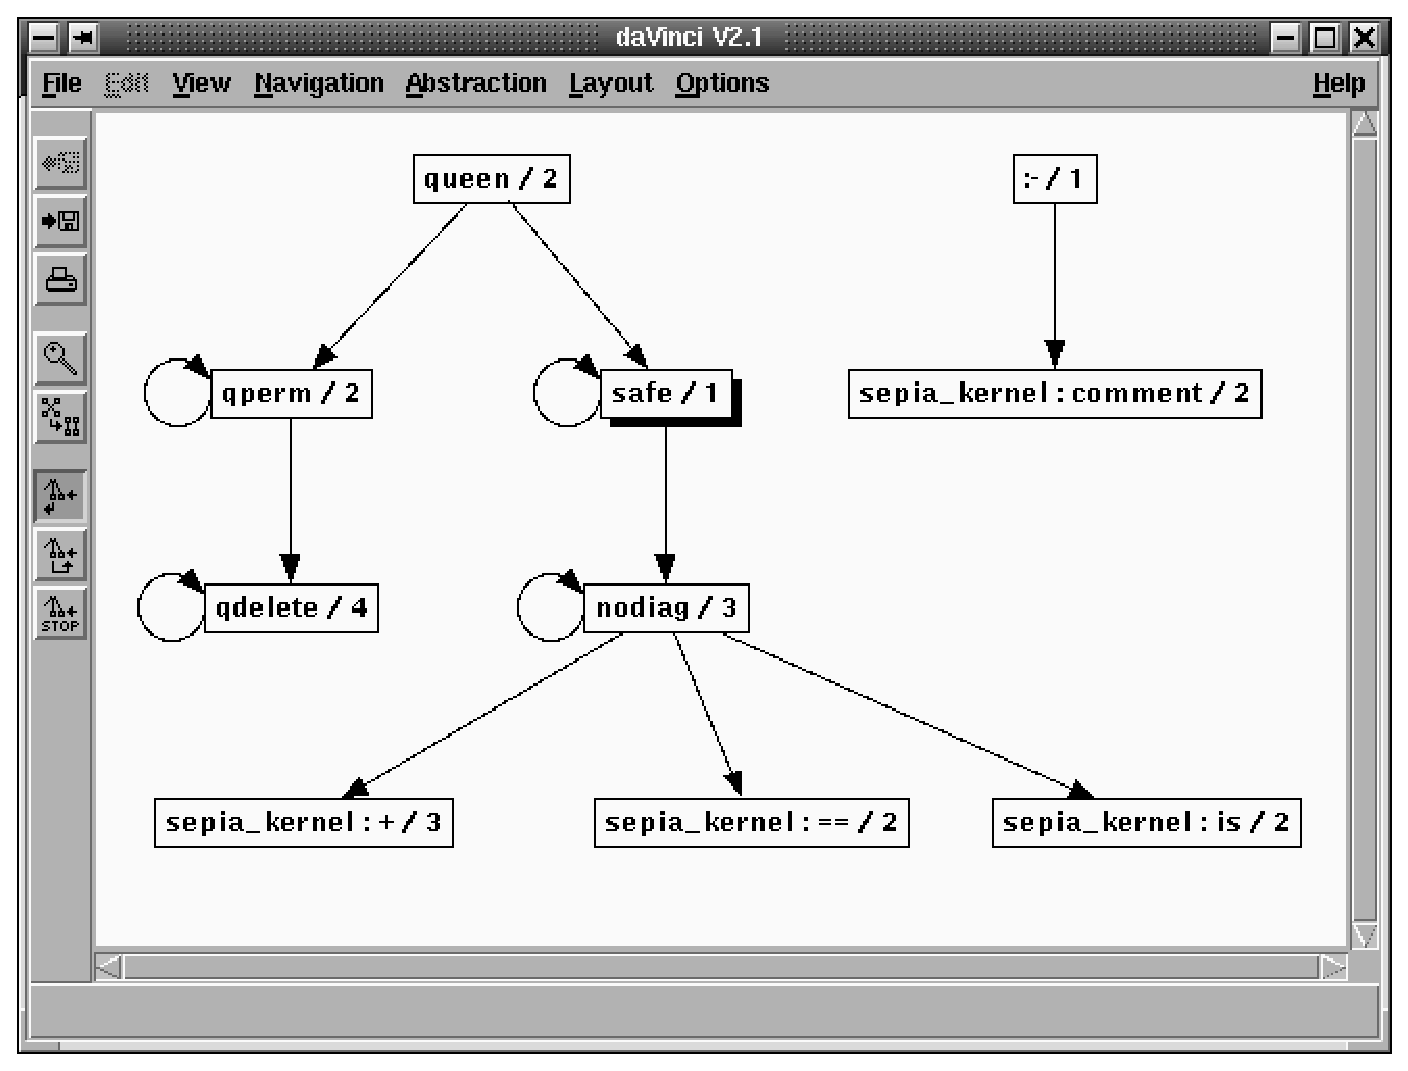
\includegraphics{xrefDavinci.eps}}
\end{center}
\caption{Call graph for queen example with built-in predicates}
\label{xrefdavinci}
\end{figure}


%----------------------------------------------------------------------
\section{Pretty Printer Tool}
%----------------------------------------------------------------------

The pretty printer library provides a set of predicates for the printing
of a file's contents as a file in a number of formats.
In particular, an {\eclipse} source file can be converted into an
HTML document with proper indentation, syntax colouring, hyperlinks
from predicate uses to definition, and hyperlinks to documentation.

The \bipref{pretty_print/2}{../bips/lib/pretty_printer/pretty_print-2.html} 
predicate is used to print the file, or list of files.
A list of options can be given which modifies the format of the output
file, its location, etc.  The following creates a {\tt pretty}
directory in the current directory. Within the pretty directory reside
{\tt index.html} and {\tt queen.html}, where {\tt queen.html} is the 
{\tt queen} module pretty printed in HTML:

\begin{quote}
\begin{verbatim}
?- pretty_printer:pretty_print(queen).
Writing /examples/pretty/queen.html
\end{verbatim}
\end{quote}


%----------------------------------------------------------------------
\section{Timing Profiler}
%----------------------------------------------------------------------

\index{profiling} The profiling tool\footnote{The profiler requires a 
small amount of hardware/compiler dependent code and may therefore not 
be available on all platforms.} helps to find \emph{hot spots} in
a program that are worth optimising. It can be used any time with any
compiled Prolog code, it is not necessary to use a special compilation
mode or set any flags.  Note however that it is not available on
Windows\index{windows}.  When
\begin{quote}\begin{verbatim}
?- profile(Goal).
\end{verbatim}\end{quote}
\index{profile/1} is called, the profiler executes the \emph{Goal} in
the profiling mode, which means that every 100th of a second the
execution is interrupted and the profiler records the currently
executing procedure.

Issuing the following query will result in the profiler recording the
currently executing goal 100 times a second.

\begin{quote}\begin{verbatim}
?- profile(queen([1,2,3,4,5,6,7,8,9],Out)).
goal succeeded

                PROFILING STATISTICS
                --------------------

Goal:             queen([1, 2, 3, 4, 5, 6, 7, 8, 9], Out)
Total user time:  0.03s

Predicate             Module        %Time   Time   %Cum
--------------------------------------------------------
qdelete           /4  eclipse       50.0%   0.01s  50.0%
nodiag            /3  eclipse       50.0%   0.01s 100.0%

Out = [1, 3, 6, 8, 2, 4, 9, 7, 5]
Yes (0.14s cpu)
\end{verbatim}\end{quote}

From the above result we can see how the profiler output contains four
important areas of information:
\begin{enumerate}
\item The first line of output indicates whether the specified goal
\textbf{succeeded}, \textbf{failed} or \textbf{aborted}.  The
\verb+profile/1+ predicate itself always succeeds.
\item The line beginning \verb+Goal:+ shows the goal which was
profiled.
\item The next line shows the time spent executing the goal.
\item Finally the predicates which were being executed when the
profiler sampled, ranked in decreasing sample count order are shown. 
\end{enumerate}

Auxiliary system predicates are printed under a
common name without arity, e.g. {\it arithmetic} or {\it 
all_solutions}.
Predicates which are local to locked modules are printed
together on a single line that contains only the module name.
By default only predicates written in Prolog are profiled, i.e.
if a Prolog predicate calls an external or built-in predicate
written in C, the time will be assigned to the Prolog predicate.

The predicate {\bf profile(Goal, Flags)} can be used to change
the way profiling is made, {\it Flags} is a list of flags.
Currently only the flag {\tt simple} is accepted and it
causes separate profiling of simple predicates, i.e.
those written in C.

The problem with the results displayed above is that the sampling
frequency is too low when compared to the total user time spent
executing the goal.  In fact in the above example the profiler was
only able to take two samples before the goal terminated.

The frequency at which the profiler samples is fixed, so in order to
obtain more representative results one should have an auxiliary
predicate which calls the goal a number of times, and compile and
profile a call to this auxiliary predicate. eg.

\begin{quote}
\begin{verbatim}
queen_100 :-
  (for(_,1,100,1) do queen([1,2,3,4,5,6,7,8,9],_Out)).
\end{verbatim}
\end{quote}

Note that, when compiled, the above \verb+do/2+ loop would be
efficiently implemented and not cause overhead that would distort the
measurement.  Section \ref{doloops} presents a 
detailed description of logical loops.

\begin{quote}\begin{verbatim}
?- profile(queen_100).
goal succeeded

                PROFILING STATISTICS
                --------------------

Goal:             queen_100
Total user time:  3.19s

Predicate             Module        %Time   Time   %Cum
--------------------------------------------------------
nodiag            /3  eclipse       52.2%   1.67s  52.2%
qdelete           /4  eclipse       27.4%   0.87s  79.6%
qperm             /2  eclipse       17.0%   0.54s  96.5%
safe              /1  eclipse        2.8%   0.09s  99.4%
queen             /2  eclipse        0.6%   0.02s 100.0%

Yes (3.33s cpu)
\end{verbatim}\end{quote}

In the above example, the profiler takes over three hundred samples
resulting in a more accurate view of where the time is being spent in
the program.  In this instance we can see that more than half of the
time is spent in the \verb+nodiag/3+ predicate, making it an ideal
candidate for optimisation.  This is left as an exercise for the
reader.


%----------------------------------------------------------------------
\section{Port Profiler}
%----------------------------------------------------------------------
\index{port_profiler (library)}
The port profiler is a performance analysis tool based on the idea of
counting of events during program execution.  The events that are
counted are defined in terms of the 'box model' of execution (the same
model that the debugger uses, see chapter \ref{boxmodel}).  In this
box model, predicates are entered though {\em call}, {\em redo} or {\em resume} ports,
and exited through {\em exit}, {\em *exit}, {\em fail} or {\em leave} ports.  In addition, other
interesting events are indicated by ports as well ({\em next}, {\em else}, {\em delay}). 

The usage is as follows: 
\begin{enumerate}
\item Compile your program in debug mode, as you would normally do during program development.
\item Load the port_profiler library 
\item Run the query which you want to examine, using port_profile/2: 
\begin{quote}\begin{verbatim}
?- port_profile(queen([1,2,3,4],Out), []).
\end{verbatim}\end{quote}
\end{enumerate}
This will print the results in a table like the following:
\begin{verbatim}
PREDICATE       CALLER               call     exit     fail    *exit     redo
-           /3  nodiag      /3         46       46        .        .        .
=\=         /2  nodiag      /3         46       45        1        .        .
qperm       /2  qperm       /2         30       28        .       16       14
qdelete     /4  qperm       /2         20       18        .       12       10
nodiag      /3  nodiag      /3         17       14        3        .        .
nodiag      /3  safe        /1         17        7       10        .        .
+           /3  nodiag      /3         17       17        .        .        .
qdelete     /4  qdelete     /4         10        9        .        3        2
qperm       /2  queen       /2          1        .        .       11       10
safe        /1  queen       /2         11        1       10        .        .
safe        /1  safe        /1          7        4        3        .        .
queen       /2  trace_body  /2          1        .        .        1        .
\end{verbatim}
Each row of the table shows the information for a particular predicate
(by default split according to different caller predicates).
The table is sorted according to entry port count ($call+redo+resume$).
The port counts give information about
\begin{itemize}
\item what are the most frequently called predicates (call ports)
\item whether predicates failed unexpectedly (fail ports)
\item whether predicates exited nondeterministically (*exit ports), i.e.
    whether they left behind any choice-points for backtracking.
\item whether nondeterministically exited predicates were ever re-entered
    to find alternative solutions (redo ports).
\item whether predicates did internal backtracking (next ports) in order
    to find the right clause. This may indicate suboptimal indexing.
\item how often predicates were delayed and resumed.
\end{itemize}
For more details about different options and output formats, see
the \bipref{Reference Manual}{../bips/lib/port_profiler/index.html}.


%----------------------------------------------------------------------
\section{Line coverage}
%----------------------------------------------------------------------
\index{library!coverage}
\index{coverage}
\index{line coverage}
The line coverage library provides a means to ascertain exactly how
many times individual clauses are called during the evaluation of a
query.

\index{coverage counters}
The library works by placing \emph{coverage counters} at strategic
points throughout the code being analysed.  These counters are
incremented each time the evaluation of a query passes them.  There
are three locations in which coverage counters can be inserted.
\begin{enumerate}
\item At the beginning of a code block.
\item Between predicate calls within a code block.
\item At the end of a code block.
\end{enumerate}
A code block is defined to be a conjunction of predicate calls. ie. a
sequence of goals separated by commas.

The counter values do not only show whether all code points were 
reached but also whether subgoals failed or aborted (in which case 
the counter before a subgoal will have a higher value than the 
counter after it).

%----------------------------------------------------------------------
\subsection{Compilation}
%----------------------------------------------------------------------
\index{ccompile/1}
\index{ccompile!coverage}
In order to add the coverage counters to code, it must be compiled with
the \bipref{ccompile/1}{../bips/lib/coverage/ccompile-1.html}
predicate which can be found in the 
\bipref{coverage}{../bips/lib/coverage/index.html} library.

The {\tt ccompile/1} predicate (note the initial `c' stands for
coverage) can be used in place of the normal {\tt compile/1}
predicate to compile a file with coverage counters.

The following shows the results of compiling the \textbf{n-queens} example:
\begin{quote}
\begin{verbatim}
?- coverage:ccompile(queen).
queen.ecl  compiled traceable 6016 bytes in 0.01 seconds
coverage: inserted 20 coverage counters into module queen 

Yes (0.14s cpu)
\end{verbatim}
\end{quote}

Once compiled, predicates can be called as usual and will (by default)
have no visible side effects. Internally however, the counters will
be incremented as the execution progresses. The following demonstrates
this for a single solution to the {\tt queen} predicate:
\begin{quote}
\begin{verbatim}
?- queen:queen([1,2,3,4,5,6,7,8,9], Out).
\end{verbatim}
\end{quote}
The counter results are retrieved as demonstrated in the subsequent section.
The two argument predicate {\tt ccompile/2} \index{ccompile/2}
\index{ccompile!coverage} can take a list of {\tt name:value} pairs
which can be used to control the exact manner in which coverage
counters are inserted. The documentation for the 
\bipref{ccompile/2}{../bips/lib/coverage/ccompile-2.html} predicate
provides for a full list of the available flags.

%----------------------------------------------------------------------
\subsection{Results}
%----------------------------------------------------------------------

\index{result/1} \index{result!coverage} To generate an HTML file
containing the coverage counter results, the 
\bipref{result/1}{../bips/lib/coverage/result-1.html} predicate is used:
\begin{quote}
\begin{verbatim}
?- coverage:result(queen).
Writing /examples/coverage/queen.html
index.pl   compiled traceable 335304 bytes in 0.17 seconds

Yes (0.18s cpu)
\end{verbatim}
\end{quote}
This creates the result file \texttt{coverage/queens.html} which
can be viewed using any browser.  It contains a pretty-printed form of
the source, annotated with the values of the code coverage counters as
described above. As a side effect, the coverage counters will be reset.

%\index{reset_counters/0} \index{reset_counters!coverage} Having
%generated and viewed results for one run, the coverage counters can be
%reset by calling the
%\bipref{reset_counters/0}{../bips/lib/coverage/reset_counters-0.html} predicate:
%\begin{quote}
%\begin{verbatim}
%?- coverage:reset_counters.
%
%Yes (0.00s cpu)
%\end{verbatim}
%\end{quote}

%----------------------------------------------------------------------
\section{Mode analysis}
%----------------------------------------------------------------------
The mode_analyser library is a tool that assists in the generation 
of the mode/1 directive for predicate definitions. This directive informs 
the compiler that the arguments of the specified predicate will always 
have the corresponding form when the predicate is called. The compiler 
utilises this information during compilation of the predicate in order 
to generate more compact and/or faster code. Specifying the mode of a 
predicate that has already been compiled has no effect, unless it is 
recompiled. If the specified procedure does not exist, a local undefined 
procedure is created.

The mode analyser inserts instrumentation into the clause definitions 
of predicates during compilation in order to record mode usage of each 
predicate argument. The code should then be run (as many times as is 
necessary to capture the most common invocations of each predicate 
undergoing analysis). Finally, the results of the analysis are requested
and the suggested mode annotations for each predicate are displayed.

The usage is as follows: 
\begin{enumerate}
\item Load the mode_analyser library:
\begin{quote}\begin{verbatim}
?- lib(mode_analyser).
\end{verbatim}\end{quote}
\item Compile your program with the mode analyser:
\begin{quote}\begin{verbatim}
?- analyse(queen).
\end{verbatim}\end{quote}
\item Run the query which most accurately exercises the 
invocation modes of the defined predicates: 
\begin{quote}\begin{verbatim}
?- queen:queen([1,2,3,4],Out).
\end{verbatim}\end{quote}
\item Generate the results for the module into which 
the program was compiled:
\begin{quote}\begin{verbatim}
?- result([verbose:on])@queen.
\end{verbatim}\end{quote}
\end{enumerate}
This will print the results as follows:
\begin{verbatim}
Mode analysis for queen : qdelete / 4:
        Results for argument 1:
                -: 23   *: 0    +: 0    ++: 0
        Results for argument 2:
                -: 0    *: 0    +: 0    ++: 23
        Results for argument 3:
                -: 0    *: 0    +: 0    ++: 23
        Results for argument 4:
                -: 0    *: 0    +: 23   ++: 0

        qdelete(-, ++, ++, +)

Mode analysis for queen : nodiag / 3:
        Results for argument 1:
                -: 0    *: 0    +: 0    ++: 62
        Results for argument 2:
                -: 0    *: 0    +: 0    ++: 62
        Results for argument 3:
                -: 0    *: 0    +: 0    ++: 62

        nodiag(++, ++, ++)

Mode analysis for queen : qperm / 2:
        Results for argument 1:
                -: 0    *: 0    +: 0    ++: 41
        Results for argument 2:
                -: 0    *: 0    +: 41   ++: 0

        qperm(++, +)

Mode analysis for queen : queen / 2:
        Results for argument 1:
                -: 0    *: 0    +: 0    ++: 1
        Results for argument 2:
                -: 1    *: 0    +: 0    ++: 0

        queen(++, -)

Mode analysis for queen : safe / 1:
        Results for argument 1:
                -: 0    *: 0    +: 0    ++: 38

        safe(++)
\end{verbatim}

NOTE: It is imperative to understand that the results of mode analysis
are merely suggestions for the invocation modes of a predicate based on
runtime information. If there are potential predicate invocation modes
that were not exercised during runtime, the tool is unable to account
for them in its analysis. For the mode specifier '-' the mode analyser
does not determine whether the variable occurs in any other argument
(i.e. is aliased), this must be manually verified.
In summary, the programmer must verify that the suggested modes are correct
before using the directive in the code.  If the instantiation of the
predicate call violates its mode declaration, no exception is raised and
its behaviour is undefined.

For more details about invocation mode analysis see 
the \bipref{Reference Manual}{../bips/lib/mode_analyser/index.html}.

%HEVEA\cutend

% BEGIN LICENSE BLOCK
% Version: CMPL 1.1
%
% The contents of this file are subject to the Cisco-style Mozilla Public
% License Version 1.1 (the "License"); you may not use this file except
% in compliance with the License.  You may obtain a copy of the License
% at www.eclipse-clp.org/license.
% 
% Software distributed under the License is distributed on an "AS IS"
% basis, WITHOUT WARRANTY OF ANY KIND, either express or implied.  See
% the License for the specific language governing rights and limitations
% under the License. 
% 
% The Original Code is  The ECLiPSe Constraint Logic Programming System. 
% The Initial Developer of the Original Code is  Cisco Systems, Inc. 
% Portions created by the Initial Developer are
% Copyright (C) 1996 - 2006 Cisco Systems, Inc.  All Rights Reserved.
% 
% Contributor(s): 
% 
% END LICENSE BLOCK

% @(#)extmeta.tex	1.8 96/01/08 
%

\chapter{Attributed Variables}
%HEVEA\cutdef[1]{section}
\label{attrvars}
\label{metaterms}
\index{attributed variables|(}

\section{Introduction}
The {\em attributed variable} is a special \eclipse data type which
represents a variable together with attached attributes.
In the literature, attributed variables are sometimes referred to as
\index{metaterms}
``metaterms''. 
The name {\em metaterm} originates from its application in meta-programming:
for an object-level program, a metaterm looks like a variable, but for
a meta-program the same variable is just a piece of data which, possibly
together with additional meta-level information, forms the metaterm.

The attributed variable is a powerful means to implement various extensions of the
plain Prolog language.
In particular, it allows the system's behaviour
on unification to be customised.
In most situations, an attributed variable behaves like a normal
variable.
E.g.\ it can be unified with other terms and \bipref{var/1}{../bips/kernel/typetest/var-1.html} succeeds on it.
The differences compared to a plain variable are:
\begin{itemize}
\item an attributed variable has a number of associated {\it attributes}
\item the attributes are included in the module system
\item when an attributed variable occurs in the unification and in some
built-in predicates, each attribute is processed by a user-defined
{\it handler}
\end{itemize}

\section{Declaration}
An attributed variable can have any number of attributes.
The attributes are accessed by their name.
Before an attribute can be created and used, it must be declared
with the predicate \bipref{meta_attribute/2}{../bips/kernel/termmanip/meta_attribute-2.html}.
The declaration has the format
\begin{quote}
{\bf meta_attribute(Name, HandlerList)}
\end{quote}
{\bf Name} is an atom denoting the attribute name
and usually it is the name of the module where this attribute
is being created and used.
{\bf HandlerList} is a (possibly empty) list of handler specifications
for this attribute (see Section \ref{metahandlers}).

\section{Syntax}

{\samepage
The most general attributed variable syntax is
\begin{quote}
$Var\{Name_1:Attr_1, Name_2:Attr_2, \ldots, Name_n:Attr_n\}$
\end{quote}
where the syntax of {\it Var} is like that of a variable,
{\it $Name_i$}
are attribute names and
{\it $Attr_i$}
are the values of the corresponding attributes.
}
The expression {\bf Var\{Attr\}} is a shorthand for {\bf Var\{Module:Attr\}}
where {\bf Module} is the current module name.
The former is called {\it unqualified} and the latter {\it qualified}
attribute specification.
\index{qualified attribute specification}
\index{attribute!specification!qualified}
\index{attribute!specification!unqualified}
As the attribute name is usually identical with the source module name,
all occurrences of an attributed variable in the source module may use the unqualified
specification.

If there are several occurrences of the same attributed variable in a single term,
only one occurrence is written with the attribute,
the others just refer to the variable's name,
e.g.
\begin{quote}\begin{verbatim}
p(X, X{attr:Attr})
\end{verbatim}\end{quote}
or
\begin{quote}\begin{verbatim}
p(X{attr:Attr}, X)
\end{verbatim}\end{quote}
both describe the same term, which has two occurrences of a single attributed variable
with attribute {\tt attr:Attr}.
The following is a syntax error (even when the attributes are identical):
\begin{quote}\begin{verbatim}
p(X{attr:Attr}, X{attr:Attr})
\end{verbatim}\end{quote}


\section{Creating Attributed Variables}
A new attribute can be added to a variable
using the tool predicate
\begin{quote}
{\bf add_attribute(Var, Attr)}.
\end{quote}
\index{add_attribute/2}
An attribute whose name is not the current module name
can be added using \bipref{add_attribute/3}{../bips/kernel/termmanip/add_attribute-3.html} which is its tool
body predicate (exported in {\tt sepia_kernel}).
If {\bf Var} is a free variable, it will be bound to a new attributed variable
whose attribute corresponding to the current module is
{\bf Attr} and all its other attributes are free variables.
If {\bf Var} is already an attributed variable and its attribute is uninstantiated,
it will be bound to {\bf Attr}, otherwise the effect of this predicate
will be the same as unifying {\bf Var} with another attributed variable
whose attribute corresponding to the current module is 
{\bf Attr}.

\section{Decomposing Attributed Variables}
The attributes of an attributed variable can be accessed using one-way
unification in a matching clause, e.g.
\begin{quote}
\begin{verbatim}
    get_attribute(X{Name:Attribute}, A) :-
        -?->
        A = Attribute.
\end{verbatim}
\end{quote}
This clause succeeds only when the first argument is an attributed variable,
and it binds
{\tt X} to the whole attributed variable and {\tt A} to the attribute
with name {\tt Name}.
Note that a normal (unification) clause can {\bf not} be used to decompose
an attributed variable (it would create a new attributed variable and unify this with the caller
argument, but the unification is handled by an attributed variable handler, see
Section \ref{metahandlers}).

\section{Attribute Modification}
Often an extension needs to modify the data stored in the
attribute to reflect changes in the computation.
The usual Prolog way to do this is by reserving
one argument in the attribute structure for this next value.
before accessing the most recent attribute value this chain
of values has to be dereferenced until a value is found whose
link is still free.
A perfect compiler should be able to detect that the older
attribute values are no longer accessed and it would compile
these modifications using destructive assignment.
Current compilers are unfortunately not able to perform
this optimization (some systems can reduce these chains
during garbage collection, but until this occurs,
the list has to be dereferenced for each access and update).
To avoid performance loss for both attribute updating and
access, {\eclipse} provides a predicate for explicit
attribute update: 
{\bf setarg(I, Term, NewArg)} will update the {\bf I}'th
argument of {\bf Term} to be {\bf NewArg}.
Its previous value will be restored on backtracking.
%Although the use of this predicate does not corrupt the
%declarative reading of the program (it is merely
%a shorthad for the above described modification
%using value links), we still recommed to use it with care,
%because sometimes it might yield unexpected results.

Libraries which define user-programmable extensions
like e.g. {\bf fd.pl} usually define predicates that
modify the attribute or a part of it, so that an explicit
use of the \bipref{setarg/3}{../bips/kernel/termmanip/setarg-3.html} predicate is not necessary.

\section{Attributed Variable Handlers}
\label{metahandlers}
An attributed variable is a variable with some additional information
which is ignored by ordinary {\it object level} system predicates.
{\it Meta level} operations on attributed variables are handled by
extensions which know
the contents of their attributes and can specify the outcome
of each operation.
This mechanism is implemented using {\it attributed variable handlers},
\index{attributed variables!handlers}
which are user-defined predicates invoked
whenever an attributed variable occurs in one of the predefined
operations.
The handlers are specified in the attribute declaration
{\bf meta_attribute(Name, HandlerList)}, the second argument
is a list of handlers in the form
\begin{quote}
\begin{verbatim}
[unify:UnifyHandler, test_unify:TUHandler, ...]
\end{verbatim}
\end{quote}
Handlers for operations which are not specified or those that are
\bipref{true/0}{../bips/kernel/control/true-0.html} are ignored and never invoked.
If {\bf Name} is an existing extension, the specified handlers
replace the current ones.

Whenever one of the specified operations detects an attributed variable,
it will invoke all handlers that were declared for it
and each of them receives either the whole attributed variable
or its particular attribute as argument.
The system does not check if the attribute that corresponds
to a given handler is instantiated or not; this means
that the handler must check itself if the attributed variable
contains any attribute information or not.
For instance, if an attributed variable {\it X\{a:_, b:_, c:f(a)\}}
is unified with the attributed variable {\it Y\{a:_, b:_, c:f(b)\}},
the handlers for the attributes {\it a} and {\it b} should
treat this as binding of two plain variables
because their attributes were not involved.
Only the handler for {\it c} has any work to do here.
The library {\bf suspend.pl} can be used as a template
\index{library!suspend.pl}
for writing attributed variable handlers.

The following operations invoke attributed variable handlers:

\begin{itemize}
%--------------------------
\item {\bf unify}: the usual unification.
\index{unify handler}
The handler procedure is
\begin{quote}
unify_handler(+Term, ?Attribute [,SuspAttr])
\end{quote}
The first argument is the term that was unified with the attributed variable,
it is either a nonvariable or an attributed variable.
The second argument is directly the contents of the attribute slot
corresponding to the extension, i.e. it is not the whole attributed variable.
When this handler is invoked, the attributed variable is already bound
to {\it Term}.
The optional third argument is the suspend-attribute of the former
variable; it may be needed to wake the variable's 'constrained' suspension
list.

If an attributed variable is unified with a standard variable, the variable is bound
to the attributed variable and no handlers are invoked.
If an attributed variable is unified with another attributed variable or a non-variable,
the attributed variable is bound (like a standard variable) to the other term
{\bf and} all handlers for the {\bf unify} operation are invoked. 
Note that several attributed variable bindings can occur e.g.\ during a head unification
and also during a single unification of compound terms.
The handlers are only invoked at certain trigger points (usually before the
next predicate call).

%--------------------------
\item {\bf test_unify}: the unification which is not supposed
\index{test_unify handler}
to trigger constraints propagation, it is used e.g.
in the \bipref{not_unify/2}{../bips/kernel/termcomp/not_unify-2.html}
predicate.
The handler procedure is
\begin{quote}
test_unify_handler(+Term, ?Attribute)
\end{quote}
where the arguments are the same as for the unify handler.
During the execution of the handler the attributed variable is bound
to {\it Term}, however when all local handlers succeed,
all bindings are undone.

\item {\bf compare_instances}: computation of instance, subsumption
\index{compare_instances handler}
and variance relationship, as performed by the built-ins
\bipref{instance/2}{../bips/kernel/termcomp/instance-2.html} and
\bipref{variant/2}{../bips/kernel/termcomp/variant-2.html}.
The handler procedure is
\begin{quote}
instance_handler(-Res, ?TermL, ?TermR)
\end{quote}
and its arguments are similar to the ones of the
\bipref{compare_instances/3}{../bips/kernel/termcomp/compare_instances-3.html}
predicate.
The handler is invoked with one or both of {\it TermL} and {\it TermR} being
attributed variables. The task of the handler is to compare the two terms
and instantiate {\bf Res} to either $=$ (if the terms are variants) or $<$
(if {\it TermL} is a proper instance of {\it TermR}). If the terms are
incomparable, the handler should fail. If {\it TermR} is proper instance
of {\it TermL}, the handler should either return $>$ or fail.
All bindings made in the handler will be undone after processing
the local handlers.

\item {\bf copy_term}: the handler is invoked when terms are copied by the
\index{copy_term handler}
\bipref{copy_term/2}{../bips/kernel/termmanip/copy_term-2.html} or
\bipref{copy_term_vars/3}{../bips/kernel/termmanip/copy_term_vars-3.html} built-ins.
The handler procedure is
\begin{quote}
copy_handler(?AttrVar, ?Copy)
\end{quote}
{\it AttrVar} is the attributed variable encountered in the
copied term, {\it Copy} is its corresponding variable in the copy.
All extension handlers receive the same arguments.
This means that if the attributed variable should be copied as
an attributed variable, the handler must check if {\it Copy} is still
a free variable or if it was already bound to an attributed variable by a previous handler.

\item {\bf suspensions}: this handler is invoked by the
\index{suspensions handler}
\bipref{suspensions/2}{../bips/kernel/suspensions/suspensions-2.html} predicate
to collect all the suspension lists inside the attribute.
The handler call pattern is
\begin{quote}
suspensions_handler(?AttrVar, -ListOfSuspLists, -Tail)
\end{quote}
{\it AttrVar} is an attributed variable. The handler should bind
{\it ListOfSuspLists} to a list containing all the attribute's
suspension lists and ending with {\it Tail}.


\item {\bf delayed_goals_number}: handler is invoked by the
\index{delayed_goals_number handler}
\bipref{delayed_goals_number/2}{../bips/kernel/suspensions/delayed_goals_number-2.html}
predicate.
The handler call pattern is
\begin{quote}
delayed_goals_number_handler(?AttrVar, -Number)
\end{quote}
{\it AttrVar} is the attributed variable encountered in the
term, {\it Number} is the number of delayed
goals occurring in this attribute.
Its main purpose is for the first-fail selection predicates,
i.e. it should return the number of constraints imposed on
the variable.

\item {\bf get_bounds}:
\index{get_bounds handler}
    This handler is used by the predicate
    \bipref{get_var_bounds/3}{../bips/kernel/termmanip/get_var_bounds-3.html}
    to retrieve information about the lower and upper bound of a numeric
    variable. 
    The handler should therefore only be defined if the attribute contains
    that kind of information. The handler call pattern is
    \begin{quote}
    get_bounds_handler(?AttrVar, -Lwb, -Upb)
    \end{quote}
    The handler is only invoked if the variable has the corresponding
    (non-empty) attribute.
    The handler should bind {\it Lwb} and {\it Upb} to numbers
    (any numeric type) reflecting the attribute's information about lower
    and upper bound of the variable, respectively.
    If different attributes return different bounds information,
    \bipref{get_var_bounds/3}{../bips/kernel/termmanip/get_var_bounds-3.html}
    will return the intersection of these bounds. This can be empty (Lwb $>$ Upb).
 
\item {\bf set_bounds}:
\index{set_bounds handler}
    This handler is used by the predicate
    \bipref{set_var_bounds/3}{../bips/kernel/termmanip/set_var_bounds-3.html}
    to distribute information about the lower and upper bound of a numeric
    variable to all its existing attributes. 
    The handler should therefore only be defined if the attribute can
    incorporate this kind of information. The handler call pattern is
    \begin{quote}
    set_bounds_handler(?AttrVar, +Lwb, +Upb)
    \end{quote}
    The handler is only invoked if the variable has the corresponding
    (non-empty) attribute.
    {\it Lwb} and {\it Upb} are the numbers that were passed to
    \bipref{set_var_bounds/3}{../bips/kernel/termmanip/set_var_bounds-3.html}, and the handler is expected to update its
    own bounds representation accordingly.



\item {\bf print}: attribute printing in
\index{print handler}
\bipref{write/1,2}{../bips/kernel/ioterm/write-1.html},
\bipref{writeln/1,2}{../bips/kernel/ioterm/writeln-1.html},
\bipref{printf/2,3}{../bips/kernel/ioterm/printf-2.html}
when the {\bf m} option is specified.
The handler procedure is
\begin{quote}
print_handler(?AttrVar, -Attribute)
\end{quote}
{\it AttrVar} is the attributed variable being printed, {\it Attribute}
is the term which will be printed as a value for this attribute,
prefixed by the attribute name.
If no handler is specified for an attribute, or the print handler fails, 
the attribute will not be printed.

\end{itemize}

The following handlers are still supported for compatibility,
but their use is not recommened:
\begin{itemize}
\item {\bf pre_unify}: this is another handler which can be invoked on
\index{pre_unify handler}
normal unification, but it is called {\it before} the unification
itself occurs.
The handler procedure is
\begin{quote}
pre_unify_handler(?AttrVar, +Term)
\end{quote}
The first argument is the attributed variable to be unfied,
the second argument is the term it is going to be unified with.
This handler is provided only for compatibility with SICStus Prolog
and its use is not recommended, because it is less efficient
than the {\bf unify} handler and because its semantics is somewhat
unclear, there may be cases where changes inside this handler
may have unexpected effects.

\item {\bf delayed_goals}: this handler is superseded by the
\index{delayed_goals handler}
suspensions-handler, which should be preferred. If there is no suspensions-
handler, this handler is invoked by the obsolete
\bipref{delayed_goals/2}{../bips/kernel/suspensions/delayed_goals-2.html} predicate.
The handler procedure is
\begin{quote}
delayed_goals_handler(?AttrVar, ?GoalList, -GoalCont)
\end{quote}
{\it AttrVar} is the attributed variable encountered in the
term, {\it GoalList} is an open-ended list of all delayed
goals in this attribute and {\it GoalCont} is the
tail of this list.

\end{itemize}

%--------------------------
\subsection{Printing Attributed Variables}
\index{output_mode}
\index{printf/2}
The different output predicates treat attributed variables differently.
The \bipref{write/1}{../bips/kernel/ioterm/write-1.html} predicate prints
the attributes using the print-handlers,
while \bipref{writeq/1}{../bips/kernel/ioterm/writeq-1.html} prints the whole attribute, so that the attributed variable
can be read back.
The \bipref{printf/2}{../bips/kernel/ioterm/printf-2.html} predicate has two options to be combined with
the {\bf w} format: {\bf M} forces the whole attributed variable to be printed
together with all its attributes in the standard format, so that
it can be read back in.
With the {\bf m} option the attributed variable is printed using the handlers
defined for the {\bf print} operation.
If there is only one handled attribute, the attributed variable is printed as
\begin{quote}
X\{Attr\}
\end{quote}
where {\it Attr} is the value obtained from the handler.
If there are several handled attributes, all attributes are qualified
like in
\begin{quote}
X\{a:A, b:B, c:C\}.
\end{quote}
{\samepage
An attributed variable {\tt X\{m:a\}} with {\bf print} handler {\bf =/2}
can thus be printed in different ways, e.g.:
\footnote{The attribute {\bf suspend} is always present and defined
by system coroutining.}
\begin{quote}\begin{verbatim}
printf("%w", [X{m:a}])   or write(X{m:a}):    X   
printf("%vMw", [X{m:a}]) or writeq(X{m:a}):   _g246{suspend : _g242, m : a}
printf("%mw", [X{m:a}]):                      X{a}
printf("%Mw", [X{m:a}]):                      X{suspend : _g251, m : a}
printf("%Vmw", [X{m:a}]):                     X_g252{a}
\end{verbatim}\end{quote}
}

\index{macro!write}
Write macros for attributed variables are not allowed because one extension alone
should not decide whether the other attributes will be printed or not.

\section{Built-Ins and Attributed Variables}
%\begin{description}
\begin{description}
\index{free/1}
\item[free(?Term)]
%\item[free(?Term)]
This type-checking predicate succeeds iff its argument is an
ordinary free variable, it fails if it is an attributed variable.

\index{meta/1}
%\item[meta(?Term)]
\item[meta(?Term)]
This type-checking predicate succeeds iff its argument is an attributed variable.
For other type testing predicates an attributed variable behaves like a variable.

%\end{description}
\end{description}

\section{Examples of Using Attributed Variables}
\subsection{Variables with Enumerated Domains}
As an example, let us implement variables of enumerable types
using attributes.
We choose to represent these variable as attributed variables
whose attribute is
a enum/1 structure with a list holding the values the variable may take,
e.g.
\begin{quote}\begin{verbatim}
X{enum([a,b,c])}
\end{verbatim}\end{quote}

We have to specify now what should happen when such a variable is
bound. This is done by writing a handler for the {\bf unify} operation.
The predicate unify_enum/2 defined below is this
handler.
Its first argument is the value that the attributed variable has been bound to,
the second is the attribute that the bound attributed variable had
(keep in mind that the system has already bound the attributed variable to the
new value).  We distinguish two cases:

First, the attributed variable has been
bound to another attributed variable (1st clause of unify_enum/2).
In this case, we form the intersection between the two lists
of admissible values. If it is empty, we fail.
If it contains exactly one value, we can instantiate the remaining
attributed variable with this value.
Otherwise, we bind it to a new attributed variable whose attribute represents
the remaining admissible values.

Second, when the attributed variable has been bound to a non-variable, the
task that remains for the handler is merely to check if this binding
was admissible (2nd clause of unify_enum/2).

\begin{quote}\begin{verbatim}
[eclipse 2]: module(enum).
warning: creating a new module in module(enum)
[enum 3]: [user].
:- meta_attribute(enum, [unify:unify_enum/2, print:print_enum/2]).
:- import setarg/3 from sepia_kernel.

% unify_enum(+Term, Attribute)
unify_enum(_, Attr) :-
    /*** ANY + VAR ***/
    var(Attr).                  % Ignore if no attribute for this extension
unify_enum(Term, Attr) :-
    compound(Attr),
    unify_term_enum(Term, Attr).

unify_term_enum(Value, enum(ListY)) :-
    nonvar(Value),               % The attributed variable was instantiated
    /*** NONVAR + META ***/
    memberchk(Value, ListY).
unify_term_enum(Y{AttrY}, AttrX) :-
    -?->
    unify_enum_enum(Y, AttrX, AttrY).

unify_enum_enum(_, AttrX, AttrY) :-
    var(AttrY),                         % no attribute for this extension
    /*** VAR + META ***/
    AttrX = AttrY.                      % share the attribute
unify_enum_enum(Y, enum(ListX), AttrY) :-
    nonvar(AttrY),
    /*** META + META ***/
    AttrY = enum(ListY),
     intersection(ListX, ListY, ListXY),
     ( ListXY = [Val] ->
            Y = Val
     ;   
            ListXY \= [],
            setarg(1, AttrY, ListXY)
     ).  

print_enum(enum(List), Attr) :-
    -?->
    Attr = List.
 user       compiled traceable 1188 bytes in 0.03 seconds

yes.
[enum 4]: A{enum([yellow, blue, white, green])}
                = B{enum([orange, blue, red, yellow])}.

A = B = A{[blue, yellow]}
yes.
[enum 5]: A{enum([yellow, blue, white, green])}
                = B{enum([orange, blue, red, black])}.

A = B = blue
yes.
[enum 6]: A{enum([yellow, blue, white, green])} = white.

A = white
yes.
[enum 7]: A{enum([yellow, blue, white, green])} = red.

no (more) solution.

\end{verbatim}
\end{quote}

Some further remarks on this code:
\index{matching}
\index{pattern matching}
\index{unification!pattern matching}
The second clause of {\bf unify_term_enum/2}
is a {\bf matching clause}, as indicated
by the ${\bf -?->}$ guard.
A matching clause is the only way to decompose an attributed variable.
Note that this clause matches only calls that have an attributed variable
with nonempty {\bf enum} attribute on the
first argument position.


\section{Attribute Specification}
The structures notation (see section~\ref{chapstruct})
is used to define
and access variable attributes and their arguments.
This makes the code independent of the number of attributes
and positions of their arguments.
Wherever appropriate, the libraries described in this document
describe their attributes in this way, e.g.
\begin{quote}
${\bf suspend\{inst:I, constrained:C, bound:B\}}$
\end{quote}
says that the structure name is {\bf suspend} and that
it has (at least) three arguments with the corresponding names.


\index{attributed variables|)}

%HEVEA\cutend



% BEGIN LICENSE BLOCK
% Version: CMPL 1.1
%
% The contents of this file are subject to the Cisco-style Mozilla Public
% License Version 1.1 (the "License"); you may not use this file except
% in compliance with the License.  You may obtain a copy of the License
% at www.eclipse-clp.org/license.
% 
% Software distributed under the License is distributed on an "AS IS"
% basis, WITHOUT WARRANTY OF ANY KIND, either express or implied.  See
% the License for the specific language governing rights and limitations
% under the License. 
% 
% The Original Code is  The ECLiPSe Constraint Logic Programming System. 
% The Initial Developer of the Original Code is  Cisco Systems, Inc. 
% Portions created by the Initial Developer are
% Copyright (C) 2006 Cisco Systems, Inc.  All Rights Reserved.
% 
% Contributor(s): 
% 
% END LICENSE BLOCK
%
% $Id: exthsusp.tex,v 1.1 2006/09/23 01:50:23 snovello Exp $
%

\chapter{Advanced Control Features}
%HEVEA\cutdef[1]{section}
\label{suspensions}

%-------
\section{Introduction}
%-------
This chapter introduces the control facilities that distinguish the
{\eclipse} language from Prolog by providing a computation
rule that is more flexible than simple left-to-right goal selection.
The core feature is the ability to suspend the execution of a goal
at some point during execution, and resume it under certain conditions
at a later stage.
Together with attributed variables, these facilities are the
prerequisites for the implementation of constraint propagation
and similar data-driven algorithms.

% Concepts
%       resolvent
%       execution model
%       floundering
% Delaying built-in predicates
% Support
% Declarative delay clauses
% The suspend predicate
% waking conditions (inst/bound/constrained, libraries, user-defined, symbolic, postponed)
% Lower-level primitives
%       The suspension 
%       making suspensions
%       attaching suspensions to variables
%       attaching suspensions to triggers
% Demons
% More about Priorities
% details of waking, cut
% simulating alternative suspension facilities
% 

%-------
\section{Concepts}
\subsection{The Structured Resolvent}
%-------
\index{resolvent}
The term {\bf resolvent} originates from Logic Programming.
It is the set of all goals that need to be satisfied.
The computation typically starts with a resolvent consisting only of the top-level goal
(the initial query).
This then gets successively transformed (by substituting goals that
match a clause head with an instance of the clause body, ie.\ a
sequence of sub-goals),
and eventually terminates with one of the trivial goals
{\bf true} or {\bf fail}.
For example, given the program
\begin{quote}\begin{verbatim}
p :- q, r.    % clause 1
q :- true.    % clause 2
r :- q.       % clause 3
\end{verbatim}\end{quote}
and the goal p, the resolvent goes through the following states
before the goal is proven (by reduction to true) and the computation terminates:
\begin{quote}\begin{verbatim}
p --1--> (q,r) --2--> (true,r) ----> (r) --3--> (q) --2--> true
\end{verbatim}\end{quote}

\index{Prolog}
While in Prolog the resolvent is always processed from left to right
like in this example,
the resolvent in {\eclipse} is more structured, and can be manipulated
in a much more flexible way.
This is achieved by two basic mechanisms, {\bf suspension}
and {\bf priorities}.

\index{suspended goal}
{\bf Suspended} goals form the part of the resolvent which is
currently not being considered. This is typically done when we
know that we cannot currently infer any interesting information from them.

\index{priority}
The remaining goals are ordered according to their {\bf priority}.
At any time, the system attempts to solve the most urgent subgoal first.
{\eclipse} currently supports a fixed range of 12 different priorities,
priority 1 being the most urgent and 12 the least urgent.

Figure \ref{figresolv} shows the structure of the resolvent.
When a toplevel goal is launched, it has priority 12 and is the only
member of the resolvent. As execution proceeds, active goals may be
suspended, and suspended goals may be woken and scheduled with a
particular priority.
\begin{figure}
% picture has been made with xfig and exported as encapsulated postscript
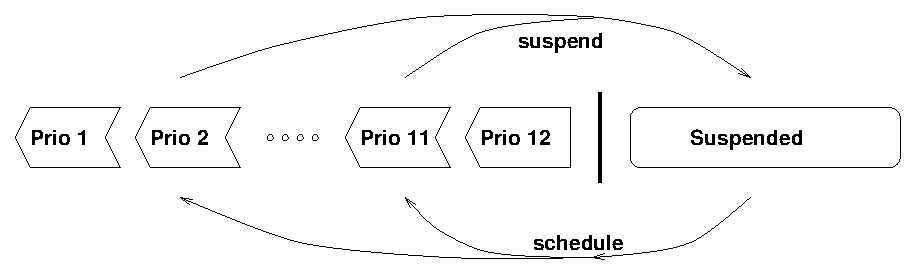
\includegraphics{resolv.eps}
\caption{Structure of the resolvent}
\label{figresolv}
\end{figure}

\subsection{Floundering}
\index{floundering}
The case that a subgoal remains suspended (delayed) at the end of the computation
\index{floundering} is sometimes referred to as {\it floundering}.
When floundering occurs, it means that the resolvent could not be reduced
to true or fail, and that the answer bindings that have been found
are valid only under the assumption that the remaining delayed goals
are in fact true. Since such a conditional answer is normally not
satisfactory (even though it may be correct), it is then necessary to change
the control aspect of the program.  The solution would usually be to either
make further variable instantiations or to change control annotations.
The aim is to get the delayed goals out of the suspended state and
into the scheduled state, where they will eventually be executed and reduced.
As a rule of thumb, goals will not suspend when all their arguments are
fully instantiated. Therefore, a program that makes sure that all its
variables are instantiated at the end of computation will typically not
suffer from floundering.


%----------------------------------------------------------------------
\section{Suspending Built-Ins and the Suspend-Library}
%----------------------------------------------------------------------

Basic {\eclipse} has two built-in predicates whose behaviour includes
suspending: the sound negation built-in
\bipref{$\sim$/1}{../bips/kernel/control/T-1.html} and the sound disequality
predicate \bipref{$\sim$=/2}{../bips/kernel/termcomp/TE-2.html}.
Instead of succeeding or failing, they will suspend when their arguments
are insufficiently instantiated to make a decision. For example
\begin{quote}\begin{verbatim}
?- X ~= 3.
X = X
There is 1 delayed goal.
Yes (0.00s cpu)
\end{verbatim}\end{quote}
Here, the system does not have enough information to decide whether the
query is true or false. The goal remains delayed and we have a case of
floundering
(the {\eclipse} toplevel indicates this situation by printing a message
about delayed goals at the end of the computation).

However, when the variable which was responsible for the suspension gets instantiated
later, the delayed goal will be resumed (woken) and either succeed, fail, or
suspend again. In the following example, the disequality predicate initially
suspends, but wakes up later and succeeds or fails, respectively:
\begin{quote}\begin{verbatim}
?- X ~= 3, X = 4.
X = 4
Yes (0.00s cpu)
?- X ~= 3, X = 3.
No (0.00s cpu)
\end{verbatim}\end{quote}


\label{suspendsolver}
Further predicate implementations with the same behaviour (delay until
all arguments are ground) can be found in the {\bf suspend library}
\index{suspend library}
\bipref{lib(suspend)}{../bips/lib/suspend/index.html}.
In particular, it implements all common arithmetic predicates plus
the constraints defined by the Common Arithmetic Solver Interface
(see Constraint Library Manual), for instance
\begin{verbatim}
=:=/2, =\=/2,  >=/2,  =</2,  >/2,  </2,
 $=/2, $\=/2, $>=/2, $=</2, $>/2, $</2,
 #=/2, #\=/2, #>=/2, #=</2, #>/2, #</2,
integers/1, reals/1,
\end{verbatim}
The solver will suspend these predicates until all their arguments
are ground\footnote{
Note that more powerful versions of these constraints exist in other
solvers such as the interval solver lib(ic).
}.

The suspend library is loaded into \eclipse\ on start-up, but the
constraints associated with the suspend solver are not imported.
To use them, either import the suspend library to the current module,
or call the constraint qualified with the module:
\begin{quote}\begin{verbatim}
suspend:(X > 2), suspend:(X #=< 5)
\end{verbatim}\end{quote}



%----------------------------------------------------------------------
\section{Development System Support}
%----------------------------------------------------------------------

As seen in the above example, the \index{top level loop} top level loop
indicates floundering by printing a message about delayed goals.
The command line toplevel then prompts and offers to print a list of
all delayed goals.
The Tkeclipse development environment provides better support in the form
of the Delayed Goals Viewer, which can be used to look at all delayed goals
or a filtered subset of them.

The tracer supports advanced control features via
the box-model ports DELAY and RESUME.
It also shows goal priorities (if they deviate from the default priority)
in angular brackets.


%----------------------------------------------------------------------
\section{Declarative Suspension: Delay Clauses}
%----------------------------------------------------------------------

For delaying calls to user-defined Prolog predicates, {\eclipse}
 provides several alternatives, the first being {\it delay clauses}.
\index{delay clauses}
Delay clauses are a declarative means (they are in fact meta-clauses)
to specify the conditions under which the predicate should delay.
The semantics of delay clauses is thus cleaner than many alternative
approaches to delay primitives.

A delay clause is very similar to a normal Prolog clause. It has the form
\begin{quote}\begin{verbatim}
delay <Head> if <Body>.
\end{verbatim}\end{quote}
A predicate may have one or more delay clauses.
They have to be textually {\bf before} and {\bf consecutive}
with the normal clauses of the predicate they belong to.
The simplest example for a delay clause is one that checks if a variable
is instantiated:
\begin{quote}\begin{verbatim}
delay report_binding(X) if var(X).
report_binding(X) :-
        printf("Variable has been bound to %w\n", [X]).
\end{verbatim}\end{quote}

%----------------------------------------------------------------------
The operational semantics of the delay clauses is as follows:
when a procedure with delay clauses is called, then the delay
clauses are executed before executing the procedure itself.
If one of the delay clauses succeeds, the call is suspended,
otherwise they are all tried in sequence and,
if all delay clauses fail, the procedure is executed as usual.

The mechanism of executing a delay clause is similar to normal Prolog
clauses with two exceptions:
\begin{itemize}
\item the unification of the goal with the delay clause head is not the usual
Prolog unification, but rather unidirectional pattern matching
(see also section \ref{matching}).
\index{pattern matching}
\index{matching}
This means that the variables in the call cannot be bound
by the matching, if such a binding would be necessary to
perform the unification, it will fail instead.
E.g. the head of the delay clause
\begin{quote}\begin{verbatim}
delay p(a, X) if var(X).
\end{verbatim}\end{quote}
does not match the goal {\bf p(A, b)} but it matches the goal {\bf p(a, b)}.

\item the delay clauses are deterministic, they leave no choice points.
If one delay clause succeeds, the call is delayed and the following delay
clauses are not executed.
As soon as the call is resumed, all delay clauses that may succeed
are re-executed.
\end{itemize}
The reason for using pattern matching instead of unification
is to avoid a possible mixing of meta-level control with the
object level, similarly to \cite{dincbas84}.


%----------------------------------------------------------------------
The form of the head of a delay clause is not restricted.
For the body, the following conditions hold:

\begin{itemize}
\item the body subgoals must not bind any variable in the call and they
must not delay themselves.
The system does not verify these conditions currently.

\item it should contain at least one of the following subgoals:
\begin{itemize}
\item \bipref{var/1}{../bips/kernel/typetest/var-1.html}
\item \bipref{nonground/1}{../bips/kernel/typetest/nonground-1.html}
\item {\bf nonground/2} (see \bipref{nonground/3}{../bips/kernel/typetest/nonground-3.html})
\item {\bf $\backslash==$/2}
\index{$\backslash==$/2}
\end{itemize}
If this is not the case, then the predicate may delay without being linked
to a variable, so it delays forever and cannot be woken again.
Experience shows that the above four primitives suffice to express most
usual conditions.
\end{itemize}

\subsubsection{More Examples}
\begin{itemize}
\item
A predicate that checks if its argument is a proper list of integers.
The delay conditions specify that the predicate should delay if the list
is not terminated or if it contains variable elements.
This makes sure that it will never generate list elements, but only
acts as a test:
\begin{quote}\begin{verbatim}
delay integer_list(L) if var(L).
delay integer_list([X|_]) if var(X).
integer_list([]).
integer_list([X|T]) :- integer(X), integer_list(T).  
\end{verbatim}\end{quote}

\item
Delay if the first two arguments are identical and the third is a variable:
\begin{quote}\begin{verbatim}
delay p(X, X, Y) if var(Y).
\end{verbatim}\end{quote}

\item
Delay if the argument is a structure whose first subterm is not ground:
\begin{quote}\begin{verbatim}
delay p(X) if compound(X), arg(1, X, Y), nonground(Y).
\end{verbatim}\end{quote}

\item
Delay if the argument term contains 2 or more variables:
\begin{quote}\begin{verbatim}
delay p(X) if nonground(2, X).
\end{verbatim}\end{quote}

\item
The
{\bf $\backslash==$/2}
\index{$\backslash==$/2}
predicate as a delaying condition is useful mainly
in predicates like X + Y = Z which need not be delayed if X == Z.
Y can be directly bound to 0, provided that X is later bound to a number
(or it is not bound at all)
The condition {\bf X {\bsl}== Y} makes sense
only if X or Y are nonground: a delay clause
\begin{quote}\begin{verbatim}
delay p(X, Y) if X \== Y.
\end{verbatim}\end{quote}
executed with the call ?- p(a, b) of course succeeds and the call delays
forever, since no variable binding can wake it.
\end{itemize}

{\bf CAUTION}: It may happen that the symbol {\bf :-} is erroneously
used instead of {\bf if} in the delay clause. To indicate this error,
the compiler complains about redefinition of the built-in predicate
{\bf delay/1}.


%----------------------------------------------------------------------
\section{Explicit supension with suspend/3}
%----------------------------------------------------------------------
\label{suspend3}
While delay-clauses are an elegant, declarative way of specifying how
a program should execute, it is sometimes necessary to be more explicit
about suspension and waking conditions.
The built-in predicate
\bipref{suspend/3}{../bips/kernel/suspensions/suspend-3.html}
is provided for this purpose\footnote{
suspend/3 is itself based on the lower-level primitives make_suspension/3
and insert_suspension/4, which are described below.}.
It allows to explicitly create a suspended goal, specify its priority
and its exact waking conditions.

When
\begin{quote}
{\bf suspend(Goal, Prio, CondList)}
\end{quote}
is called, {\it Goal} will be suspended with priority {\it Prio}
and it will wake up
as soon as one of the conditions specified in the {\it CondList}
is satisfied.
This list contains specifications of the form
\begin{quote}
{\bf Vars $->$ Cond}
\end{quote}
to denote that as soon as one of the variables in the term {\it Vars}
satisfies the condition {\it Cond}, the suspended goal will
be woken and then executed as soon as the program priority allows it.
{\it CondList} can also be a single specification.

The condition {\it Cond} can be the name of a system-defined waking condition,
e.g.
\begin{quote}\begin{verbatim}
[X,Y]->inst
\end{verbatim}\end{quote}
means that as soon as one (or both) of the variables {\bf X, Y}
is instantiated, the suspended goal will be woken.
\index{suspending variables}
These variables are also called the {\it suspending variables} of the goal.


Cond can also be the specification of a suspension list
defined in one of currently loaded library attributes. E.g. when the
interval solver library lib(ic) is loaded, either of
\begin{quote}\begin{verbatim}
[A,B]->ic:min
[A,B]->ic:(min of ic)
\end{verbatim}\end{quote}
triggers the suspended goal as soon as the minimum element
of the domain of either {\bf A} or {\bf B} are updated
(see Constraint Library Manual, IC Library).

Another admissible form of condition {\it Cond} is
\begin{quote}\begin{verbatim}
trigger(Name)
\end{verbatim}\end{quote}
which suspends the goal on the global trigger condition {\bf Name}
(see section~\ref{trigger}).


Using
\bipref{suspend/3}{../bips/kernel/suspensions/suspend-3.html},
we can rewrite our first delay-clause example from above as follows:
\begin{quote}\begin{verbatim}
report_binding(X) :-
        ( var(X) ->
            suspend(report_binding(X), 0, X->inst)
        ;
            printf("Variable has been bound to %w\n", [X])
        ).
\end{verbatim}\end{quote}
Here, when the predicate is called with an uninstantiated argument,
we explicitly suspend a goal with the condition that it be woken as
soon as X becomes instantiated. The priority is given as 0, which indicates
the default priority (0 is not a valid priority itself).
Running this code produces the following:
\begin{quote}\begin{verbatim}
?- report_binding(X).
X = X
There is 1 delayed goal.
Yes (0.00s cpu)
\end{verbatim}\end{quote}
When X is later instantiated, it will wake up and print the message:
\begin{quote}\begin{verbatim}
?- report_binding(X), writeln(here), X = 99.
here
Variable has been bound to 99
X = 99
Yes (0.00s cpu)
\end{verbatim}\end{quote}



%----------------------------------------------------------------------
\section{Waking conditions}
%----------------------------------------------------------------------
The usual purpose of suspending a goal is to wait and resume it later
when more information about its arguments is available.
In Logic Programming, this is usually the case when certain events
related to variables occur.
When such an event occurs, the suspended goal is passed to the
waking scheduler which puts it at the appropriate place
in the priority queue of woken goals and as soon as it becomes
first in the queue, the suspended goal is executed.

The event which causes a suspended goal to be woken is usually
related to one or more variables, for example
variable instantiation, or a modification of a variable's
attribute.
However, it is also possible to trigger suspension with symbolic events
not related to any variable.


%----------------------------------------------------------------------
\subsection{Standard Waking Conditions on Variables}
%----------------------------------------------------------------------
\label{suspend}
\index{suspend}
\index{coroutining}
\label{coroutining}%
There are three very general standard waking conditions which
can be used with any variable. They are, in order of increasing generality:
\begin{description}
\item[{\bf inst:}] wake when a variable gets instantiated
\item[{\bf bound:}] wake when a variable gets instantiated or bound to
        another variable
\item[{\bf constrained:}] wake when a variable gets instantiated or bound to
        another variable or becomes otherwise constrained 
\end{description}
Each condition subsumes the preceding, more specific ones.


% - - - - - - - - - - - - - - - - - - - - - - - - - - - - - - - - - -
\subsubsection{Waking on Instantiation: inst}
% - - - - - - - - - - - - - - - - - - - - - - - - - - - - - - - - - -

To wake a goal when a variable gets instantiated, the {\bf inst}
condition is used. For example the following code suspends a goal until
variable X is instantiated:
\begin{quote}\begin{verbatim}
?- suspend(writeln(woken(X)), 0, X->inst).
X = X
There is 1 delayed goal.
Yes (0.00s cpu)
\end{verbatim}\end{quote}
If this variable is later instantiated (bound to a non-variable),
the goal executes in a data-driven way:
\begin{quote}\begin{verbatim}
?- suspend(writeln(woken(X)), 0, X->inst), X = 99.
woken(99)
X = 99
Yes (0.00s cpu)
\end{verbatim}\end{quote}
If we specify several instantiation conditions for the same goal,
the goal will wake up as soon as the first of them occurs:
\begin{quote}\begin{verbatim}
?- suspend(writeln(woken(X,Y)), 0, [X,Y]->inst), X = 99.
woken(99, Y)
X = 99
Y = Y
Yes (0.00s cpu)
\end{verbatim}\end{quote}
It is not possible to specify a conjunction of conditions directly!

Let us now suppose we want to implement a predicate succ(X,Y) which
is true when Y is the next integer after X. If we want the predicate
to act as a lazy test, we need to let it suspend until both variables
are instantiated. This can be programmed as follows:
\begin{quote}\begin{verbatim}
succ_lazy(X, Y) :-
        ( var(X) -> suspend(succ_lazy(X,Y), 0, X->inst)
        ; var(Y) -> suspend(succ_lazy(X,Y), 0, Y->inst)
        ; Y =:= X+1
        ).
\end{verbatim}\end{quote}
The conjunctive condition "wait until X and Y are instantiated" is
implemented by first waiting for X's instantiation, then waking up and
re-suspending waiting for Y's instantiation.

A more eager implementation of succ/2 would delay only until
a single variable argument is left, and then compute the variable from
the nonvariable argument:
\begin{quote}\begin{verbatim}
succ_eager(X, Y) :-
        ( var(X) ->
            ( var(Y) ->
                suspend(succ_eager(X,Y), 0, [X,Y]->inst)
            ;
                X is Y-1
            )
        ;
            Y is X+1
        ).
\end{verbatim}\end{quote}
Here, we suspend only in the case that both arguments are variables,
and wake up as soon as either of them gets instantiated.

Waiting for groundness of a term can be done in a way similar to the
way succ_lazy/2 waited for both arguments to be instantiated: we pick
any variable in the nonground term and wait for its instantiation.
If this happens, we check whether other variables remain, and if yes,
we re-suspend on one of the remaining variables. The following predicate
waits for a term to become ground, and then calls arithmetic evaluation on it:
\begin{quote}\begin{verbatim}
eval_lazy(Expr, Result) :-
        ( nonground(Expr, Var) ->
            suspend(eval_lazy(Expr,Result), 0, Var->inst)
        ;
            Result is Expr
        ).
\end{verbatim}\end{quote}
We have used the built-in predicate
\bipref{nonground/2}{../bips/kernel/typetest/nonground-2.html}
which tests a term for groundness and returns one of its variables
if it is nonground. Note also that in this implementation the same
\verb.eval_lazy/2. goal gets woken and re-suspended possibly many times.
See section \ref{secdemon} below for how to address this inefficiency.


% - - - - - - - - - - - - - - - - - - - - - - - - - - - - - - - - - -
\subsubsection{Waking on Binding: bound}
% - - - - - - - - - - - - - - - - - - - - - - - - - - - - - - - - - -

Sometimes it is interesting to wake a goal when the number of variables
among its arguments is reduced. This happens not only when a variable
disappears due to instantiation, but also when two variables get unified
(the result being a single variable). Consider the succ_eager/2 predicate
above: we know that a goal like \verb.succ_eager(X,X). must always fail
because an integer cannot be equal to its successor. However, the above
implementation does not detect this case until X gets instantiated.

The {\bf bound} waking condition subsumes the {\bf inst} condition, but
also wakes when any two of the variables in the condition specification get
unified with each other (aliased).
Using this property, we can improve the implementation of succ_eager/2
as follows:
\begin{quote}\begin{verbatim}
succ_eager1(X, Y) :-
        ( var(X) ->
            ( var(Y) ->
                X \== Y,
                suspend(succ_eager1(X,Y), 0, [X,Y]->bound)
            ;
                X is Y-1
            )
        ;
            Y is X+1
        ).
\end{verbatim}\end{quote}
This gives us the desirable behaviour of failing as soon as possible:
\begin{quote}\begin{verbatim}
?- succ_eager1(X, Y), X = Y.
No (0.00s cpu)
\end{verbatim}\end{quote}
Note that the built-in predicate
\bipref{$\sim$=/2}{../bips/kernel/termcomp/TE-2.html}
is a similar case and uses the {\bf bound} waking condition for the
same reason.



% - - - - - - - - - - - - - - - - - - - - - - - - - - - - - - - - - -
\subsubsection{Waking on Constraining: constrained}
% - - - - - - - - - - - - - - - - - - - - - - - - - - - - - - - - - -

In plain Prolog, variable instantiation is the only way in which a single
variable can become more constrained.  In the presence of constraints,
there are other ways. The most obvious example are variable domains:
when a variable's domain gets reduced, the variable becomes more
constrained. This means that a delayed goal that previously still had
a chance to succeed, could now have become impossible to satisfy,
and should therefore be checked again.

The purpose of the {\bf constrained} waking condition is to make it
possible to wake a suspended goal whenever a variable becomes more
constrained in a general sense. Having this general notion
of constrained-ness makes it possible to write generic libraries
that do interesting things with constraints and constrained variables
without their implementation having to be linked to a particular
constraint-solver\footnote{Examples of such libraries are branch_and_bound,
changeset, chr/ech, propia, repair, visualisation.}.

The {\bf constrained} waking condition subsumes the {\bf bound} condition
(which in turn subsumes the {\bf inst} condition). 
While goals suspended on the {\bf inst} and {\bf bound} conditions
are woken implicitly by the unification routine, libaries which implement
domain variables are responsible for notifying the system when they
constrain a variable. They do so by invoking the built-ins
\bipref{notify_constrained/1}{../bips/kernel/suspensions/notify_constrained-1.html}
and \bipref{wake/0}{../bips/kernel/suspensions/wake-0.html}
which is the generic way of telling the system that a variable has been
constrained.

The simplest application using the {\bf constrained} condition is a little
debugging support predicate that prints a variable's current partial value
(e.g. domain) whenever it changes:
\begin{quote}\begin{verbatim}
report(X) :-
        ( var(X) ->
            writeln(constrained(X)),
            suspend(report(X), 1, X->constrained)  % (re)suspend
        ;
            writeln(instantiated(X))
        ).
\end{verbatim}\end{quote}
This now works with any library that implements a notion of constrainedness,
e.g.\ the interval solver library(ic):
\begin{quote}\begin{verbatim}
?- report(X), X :: 1..5, X #> 2, X #< 4.
constrained(X)
constrained(X{1 .. 5})
constrained(X{3 .. 5})
instantiated(3)
X = 3
Yes (0.01s cpu)
\end{verbatim}\end{quote}
The report/1 predicate is woken when the domain is initally attached to X,
whenever the domain gets reduced, and finally when X gets instantiated.



%----------------------------------------------------------------------
\subsection{Library-defined Waking Conditions on Variables}
%----------------------------------------------------------------------

Constraint-solver libraries typically define additional, specialised
waking conditions for the type of variable that they implement.
For instance, the interval solver lib(ic) defines the following
conditions:
\begin{description}
\item[min] wake when the minimum domain value changes
\item[max] wake when the maximum domain value changes
\item[hole] wake when the domain gets a new hole
\item[type] wake when the variable type changes from real to integer
\end{description}
Obviously, these conditions only make sense for domain variables
that are created by the lib(ic) library, and are mainly useful for
implementing extensions to this library, e.g.\ new constraints.
The library-defined waking conditions can be used with
\bipref{suspend/3}{../bips/kernel/suspensions/suspend-3.html}
by using one of the following syntactic forms:
\begin{quote}\begin{verbatim}
[A, B]->ic:min
[A, B]->ic:(min of ic)
\end{verbatim}\end{quote}
Using these conditions, we can define a more specialised form of
the above report/1 predicate which only wakes up on the specified
ic-domain changes:
\begin{quote}\begin{verbatim}
report_ic(X) :-
        ( var(X) ->
            writeln(newdomain(X)),
            suspend(report_ic(X), 1, [X->ic:min,X->ic:max,X->ic:hole])
        ;
            writeln(instantiated(X))
        ).
\end{verbatim}\end{quote}
The behaviour is similar to above, the predicate wakes up on every
domain change:
\begin{quote}\begin{verbatim}
?- X::1..5, report_ic(X), X#> 2, X #< 4.
newdomain(X{1 .. 5})
newdomain(X{3 .. 5})
instantiated(3)
X = 3
Yes (0.00s cpu)
\end{verbatim}\end{quote}
Note that we now have to set up the delayed goal {\em after} the
variable already has a domain. This is because the ic-specific waking
conditions can only be used with ic-variables\footnote{more precisely,
variables which have an ic-attribute, see chapter \ref{attrvars}.},
not with domain-less generic variables.



%----------------------------------------------------------------------
\subsection{Global Symbolic Waking Conditions: Triggers}
\label{trigger}
%----------------------------------------------------------------------

Although waking conditions for a goal are usually related to variables
within the goal's arguments, it is also possible to specify symbolic
waking conditions which are unrelated to variables.
\index{trigger}\index{symbolic waking condition}%
These are called {\bf triggers} and are identified simply by an
arbitrary name (an atom). Goals can be suspended on such triggers,
and the trigger can be pulled explicitly by program code in
particular circumstances. By combining triggers with the event mechanism
\index{events}
(chapter \ref{chapexcept}) it is even possible to wake goals in
response to synchronous or asynchronous events.

A goal is suspended on a trigger using the syntax {\bf trigger(Name)}
in \bipref{suspend/3}{../bips/kernel/suspensions/suspend-3.html}
as in the following example:
\begin{quote}\begin{verbatim}
?- suspend(writeln(woken), 0, trigger(happy)).
There is 1 delayed goal.
Yes (0.00s cpu)
\end{verbatim}\end{quote}
The built-in
\bipref{trigger/1}{../bips/kernel/suspensions/trigger-1.html}
can then be used to wake the goal:
\begin{quote}\begin{verbatim}
?- suspend(writeln(woken), 0, trigger(happy)), trigger(happy).
woken
Yes (0.00s cpu)
\end{verbatim}\end{quote}
Of course, symbolic triggers can be used together with other
waking conditions to specify alternative reasons to wake a goal.



% - - - - - - - - - - - - - - - - - - - - - - - - - - - - - - - - - -
\subsubsection{Postponed Goals}
% - - - - - - - - - - - - - - - - - - - - - - - - - - - - - - - - - -
\index{postponed}
There is one system-defined trigger called {\bf postponed}.
It is provided as a way to postpone the triggering of a goal as much
as possible. This trigger is pulled just before the end of
certain encapsulated executions, like
\begin{itemize}
\item end of toplevel execution
\item inside all-solution predicates (\bipref{findall/3}{../bips/kernel/allsols/findall-3.html}, \bipref{setof/3}{../bips/kernel/allsols/setof-3.html})
\item inside \bipref{bb_min/3}{../bips/lib/branch_and_bound/bb_min-3.html} and \bipref{minimize/2}{../bips/lib/branch_and_bound/minimize-2.html}
\end{itemize}
A suspension should be attached to the {\bf postponed} trigger only when
\begin{itemize}
\item it might not have any other waking conditions left
\item and it might at the same time have other waking conditions left
        that could make it fail during further execution
\item and one does not want to execute it now, e.g.\ because it is known
        to succeed or re-suspend
\end{itemize}
An example is a goal that originally woke on modifications of the upper
bound of an interval variable. If the variable gets instantiated to its
upper bound, there is no need to wake the goal (since the bound has not
changed), but the variable (and with it the waking condition) disappears
and the goal may be left orphaned.




%----------------------------------------------------------------------
\section{Lower-level Primitives}
%----------------------------------------------------------------------

Suspended goals are actually represented by a special
opaque data type, called {\bf suspension}, which can be explicitly
manipulated under program control using the primitives defined in
this section.
Although usually a suspended goal waits for some waking condition
in order to be reactivated, the primitives for suspension handling
do not enforce this. To provide maximum flexibility of use,
the functionalities of suspending and waking/scheduling are
separated from the trigger mechanisms that cause the waking. 


\index{suspension|(}

\subsection{Suspensions and Suspension Lists}
%-------
A suspension represents a goal that is part of the resolvent.
Apart from the goal structure proper, it holds information that
is used for controlling its execution.
The components of a suspension are:
\begin{description}
\item[The goal structure]
        A term representing the goal itself, eg.\ {\em X \gt Y}.
\item[The goal module]
        The module from which the goal was called.
\item[The goal priority]
        The priority with which the goal will be scheduled when
        it becomes woken.
\item[The state]
        This indicates the current position of the suspension within
        the resolvent. It is either suspended (sleeping), scheduled
	or executed (dead).
\item[Additional data]
	E.g. debugging information.
\end{description}

Suspensions which should be woken by the same event are grouped
together in a {\it suspension list}.
\index{suspension list}
%This is a normal Prolog list which contains suspensions.
Suspension lists are either stored in an attribute of
an attributed variable or attached to a symbolic trigger.


\subsection{Creating Suspended Goals}
%-------
\index{suspension!creating}
The most basic primitive to create a suspension is
\biptxtref{make_suspension(Goal, Priority, Susp \lbr, Module\rbr)}{make_suspension/3,4}{../bips/kernel/suspensions/make_suspension-3.html}
where {\bf Goal} is the goal structure,
{\bf Priority} is a small integer denoting the priority with which
the goal should be woken and {\bf Susp} is the resulting suspension.

Note that usually
\bipref{make_suspension/3,4}{../bips/kernel/suspensions/make_suspension-3.html}
is not used directly, but implicitly via
\bipref{suspend/3,4}{../bips/kernel/suspensions/suspend-3.html} 
(described in section \ref{suspend3}) which in addition attaches the suspension to a
trigger condition.

A suspension which has not yet been scheduled
for execution and executed, is called {\em sleeping},
\index{suspension!sleeping}
a suspension which has already been executed is called
{\em executed} or {\em dead} (since it disappears from the resolvent,
but see section \ref{secdemon} for an exception).
\index{suspension!executed}
A newly created suspension is always sleeping, however
note that due to backtracking, an executed suspension
can become sleeping again.
\index{suspension!waking}
Sometimes we use the term {\em waking}, which is less precise and
denotes the process of both scheduling and eventual execution.


By default, suspensions are printed as follows (the variants with invocation
numbers are used when the debugger is active):
\begin{center}
\begin{tabular}{|c|l|}
\hline
'SUSP-_78-susp'		&	sleeping suspension with id _78 \\
'SUSP-_78-sched'	&	scheduled suspension with id _78 \\
'SUSP-_78-dead'		&	dead suspension with id _78 \\
\hline
'SUSP-123-susp'		&	sleeping suspension with invocation number 123 \\
'SUSP-123-sched'	&	scheduled suspension with invocation number 123 \\
'SUSP-123-dead'		&	dead suspension with id invocation number 123 \\
\hline
\end{tabular}
\end{center}
It is possible to change the way suspensions are printed by defining a 
\bipref{portray/3}{../bips/kernel/syntax/portray-3.html}
transformation for the term type {\tt goal}.



\subsection{Operations on Suspensions}
%-------
The following summarises the predicates that can be used to create, test,
decompose and destroy suspensions.
\begin{description}
\item[\biptxtref{make_suspension(Goal, Priority, Susp)}{make_suspension/3}{../bips/kernel/suspensions/make_suspension-3.html}]
\item[\biptxtref{make_suspension(Goal, Priority, Susp, Module)}{make_suspension/4}{../bips/kernel/suspensions/make_suspension-4.html}]
Create a suspension {\bf Susp} with a given priority from a given goal.
The goal will subsequently show up as a {\it delayed goal}.

\item[\biptxtref{is_suspension(Susp)}{is_suspension/1}{../bips/kernel/typetest/is_suspension-1.html}]
Succeeds if {\bf Susp} is a sleeping or scheduled suspension,
fails if it is not a suspension or a suspension that has been already executed.

\item[\biptxtref{type_of(S, goal)}{type_of/2}{../bips/kernel/typetest/type_of-2.html}]
Succeeds if {\bf S} is a suspension, no matter if it is
sleeping, scheduled or executed.

\item[\biptxtref{get_suspension_data(Susp, Name, Value)}{get_suspension_data/3}{../bips/kernel/suspensions/get_suspension_data-3.html}]
Extract any of the information contained in the suspension:
{\bf Name} can be one of
\verb.goal., \verb.module., \verb.priority., \verb.state. or \verb.invoc. (debugger invocation number).


\item[\biptxtref{set_suspension_data(Susp, Name, Value)}{set_suspension_data/3}{../bips/kernel/suspensions/set_suspension_data-3.html}]
The \verb.priority. and \verb.invoc. (debugger invocation number) fields
of a suspension can be changed using this primitive.
If the priority of a sleeping suspension is changed,
this will only have an effect at the time the suspension gets
scheduled. If the suspension is already scheduled, changing
priority has no effect, except for future schedulings of demons
(see~\ref{secdemon}).


\item[\biptxtref{kill_suspension(Susp)}{kill_suspension/1}{../bips/kernel/suspensions/kill_suspension-1.html}]
Convert the suspension {\bf Susp} into an {\it executed}
one, ie.\ remove the suspended goal from the resolvent.
This predicate is meta-logical as its use may
change the semantics of the program.
\end{description}



\subsection{Examining the Resolvent}
%-------
The system keeps track of all created suspensions and it
uses this data e.g.\ in the built-in predicates
\bipref{delayed_goals/1}{../bips/kernel/suspensions/delayed_goals-1.html},
\bipref{suspensions/1}{../bips/kernel/suspensions/suspensions-1.html},
\bipref{current_suspension/1}{../bips/kernel/suspensions/current_suspension-1.html},
\bipref{subcall/2}{../bips/kernel/suspensions/subcall-2.html}
\index{floundering}
and to detect floundering of the query given to the {\eclipse} top-level loop.



\subsection{Attaching Suspensions to Variables}
%---------


Suspensions are attached to variables by means of the attribute mechanism.
\index{attribute}
For this purpose, a variable attribute needs to have one or more slots
reserved for {\bf suspension lists}.
\index{suspension list}
Suspensions can then be inserted into one or several of those lists using
\begin{description}
\item[\biptxtref{insert_suspension(Vars, Susp, Index)}{insert_suspension/3}{../bips/kernel/suspensions/insert_suspension-3.html}]
Insert the suspension {\bf Susp} into the {\bf Index}'th
suspension list of all attributed variables occurring in {\bf Vars}.
The current module specifies which of the attributes will be taken.

\item[\biptxtref{insert_suspension(Vars, Susp, Index, Module)}{insert_suspension/4}{../bips/kernel/suspensions/insert_suspension-4.html}]
Similar to \bipref{insert_suspension/3}{../bips/kernel/suspensions/insert_suspension-3.html},
but it inserts the suspension into the attribute specified by {\bf Module}.
\end{description}

For instance,
\begin{quote}\begin{verbatim}
insert_suspension(Vars, Susp, inst of suspend, suspend)
\end{verbatim}\end{quote}
inserts the suspension into the {\bf inst}%
list of the (system-predefined) {\bf suspend}
attribute of all variables that occur in {\bf Vars}, and
\begin{quote}\begin{verbatim}
insert_suspension(Vars, Susp, max of fd, fd)
\end{verbatim}\end{quote}
would insert the suspension into the {\bf max} list of the finite-domain
attribute of all variables in {\bf Vars}.

Note that both predicates
find all attributed variables which occur in the general term {\bf Vars} and for each of them,
locate the attribute which corresponds to the current module or the
{\bf Module} argument respectively.
This attribute must be a structure, otherwise an error
is raised, which means that the attribute has to be initialised
before calling
\bipref{insert_suspension/4,3}{../bips/kernel/suspensions/insert_suspension-4.html}.
Finally, the {\bf Index}'th argument of the attribute
is interpreted as a suspension list and the suspension
{\bf Susp} is inserted at the beginning of this list.
%\bipref{insert_suspension/3}{../bips/kernel/suspensions/insert_suspension-3.html} also recognises suspension
%lists which are difference lists, i.e. terms {\it Start - Tail}.
A more user-friendly interface to access suspension lists is
provided by the
\bipref{suspend/3}{../bips/kernel/suspensions/suspend-3.html}
predicate.


\subsection{User-defined Suspension Lists}

Many important attributes and suspension lists are either provided by
the suspend-attribute or by libraries like the interval solver library lib(ic).
For those suspension lists, initialisation and waking is taken care of
by the library code.

For the implementation of user-defined suspension lists,
the following low-level primitives are provided:
\begin{description}
\item[\biptxtref{init_suspension_list(+Position, +Attribute)}{init_suspension_list/2}{../bips/kernel/suspensions/init_suspension_list-2.html}]
    Initialises argument Position of Attribute to an empty suspension list.
\item[\biptxtref{merge_suspension_lists(+Pos1, +Attr1, +Pos2, +Attr2)}{merge_suspension_lists/4}{../bips/kernel/suspensions/merge_suspension_lists-4.html}]
    Destructively appends the first suspension list (argument Pos1 of Attr1) to
    the end of the second (argument Pos2 of Attr2).
\item[\biptxtref{enter_suspension_list(+Pos, +Attr, +Susp)}{enter_suspension_list/3}{../bips/kernel/suspensions/enter_suspension_list-3.html}]
    Adds the suspension Susp to the suspension list in the
    argument position Pos of Attr. The suspension list can be pre-existing,
    or the argument could be uninstantiated, in which case a new suspension
    list will be created.
\item[\biptxtref{schedule_suspensions(+Position, +Attribute)}{schedule_suspensions/2}{../bips/kernel/suspensions/schedule_suspensions-2.html}]
    Takes the suspension list on argument position {\bf Position} within
    {\bf Attribute}, and schedule them for execution. 
    As a side effect, the suspension list within {\bf Attribute} is updated,
    ie.\ suspensions which are no longer useful are removed destructively.
    See section \ref{secwaking} for more details on waking.
\end{description}


\subsection{Attaching Suspensions to Global Triggers}
%---------
\index{trigger}
\index{symbolic waking condition}
A single suspension or a list of suspensions can be attached to a
symbolic trigger by using
\biptxtref{attach_suspensions(+Trigger, +Susps)}{attach_suspensions/2}{../bips/kernel/suspensions/attach_suspensions-2.html}.
A symbolic trigger can have an arbitrary name (an atom).
%To "pull the trigger"
%\biptxtref{schedule_suspensions(+Trigger)}{schedule_suspensions/1}{../bips/kernel/suspensions/schedule_suspensions-1.html}
%is used which will submit all attached suspensions to the waking scheduler.




%-------
\subsection{Scheduling Suspensions for Waking}
%-------
\label{secwaking}\index{waking}%
Suspended goals are woken by submitting at least one of the suspension lists
in which they occur to the waking scheduler.
The waking scheduler which maintains a global priority queue inserts
them into this queue according to their priority (see figure \ref{figresolv}).
A suspension list can be passed to the scheduler by either of the predicates
\bipref{schedule_suspensions/1}{../bips/kernel/suspensions/schedule_suspensions-1.html}
(for triggers)
or
\bipref{schedule_suspensions/2}{../bips/kernel/suspensions/schedule_suspensions-2.html}
(for uder-defined suspension lists).
A suspension which has been scheduled in this way and awaits
its execution is called a {\it scheduled suspension}.

Note, however, that scheduling a suspension by means of
\bipref{schedule_suspensions/1}{../bips/kernel/suspensions/schedule_suspensions-1.html}
or
\bipref{schedule_suspensions/2}{../bips/kernel/suspensions/schedule_suspensions-2.html}
alone does not implicitly start the waking scheduler.
Instead, execution continues normally with the next goal in sequence after
schedule_suspensions/1,2.
The scheduler must be explicitly invoked by calling 
\bipref{wake/0}{../bips/kernel/suspensions/wake-0.html}.
Only then does it start to execute the woken suspensions.

The reason for having \bipref{wake/0}{../bips/kernel/suspensions/wake-0.html}
is to be able to schedule several suspension lists before the
priority-driven execution begins%
\footnote{This mechanism may be reconsidered in a future release}.

\index{suspension|)}


%----------------------------------------------------------------------
\section{Demon Predicates}
%----------------------------------------------------------------------
\label{secdemon}%
A common pattern when implementing data-driven algorithms is the following
variant of the report/1 example from above:
\begin{quote}\begin{verbatim}
report(X) :-
      suspend(report1(X), 1, X->constrained).      % suspend

report1(X) :-
        ( var(X) ->
            writeln(constrained(X)),
            suspend(report(X), 1, X->constrained)  % re-suspend
        ;
            writeln(instantiated(X))               % die
        ).
\end{verbatim}\end{quote}
Here we have a goal that keeps monitoring changes to its variables.
To do so, it suspends on some or all of those variables.
When a change occurs, it gets woken, does something, and re-suspends.
The repeated re-suspending has two disadvantages: it can be inefficient,
and the goal does not have a unique identifying suspension that could be
easily referred to, because on every re-suspend a new suspension is created.

To better support this type of goals, {\eclipse} provides a special type
of predicate, called a {\bf demon}. A predicate is turned into a
\index{demon}
demon by annotating it with a
\bipref{demon/1}{../bips/kernel/database/demon-1.html}
declaration.
A demon goal differs from a normal goal only in its behaviour on
waking. While a normal goal disappears from the resolvent when it is
woken, the demon remains in the resolvent.
Declaratively, this corresponds to an implicit recursive call in
the body of each demon clause.
Or, in other words, the demon goal forks into one goal that remains in the
suspended part of the resolvent, and an identical one
that gets scheduled for execution.

With this functionality, our above example can be done more
efficiently. One complication arises, however. Since the goal
implicitly re-suspends, it now has to be explicitly killed when
it is no longer needed. The easiest way to achieve this is to
let it remember its own suspension in one of its arguments.
This can then be used to kill the suspension when required:
\begin{quote}\begin{verbatim}
% A demon that wakes whenever X becomes more constrained
report(X) :-
      suspend(report(X, Susp), 1, X->constrained, Susp).

:- demon(report/2).
report(X, _Susp) :-
      ( var(X) ->
          writeln(constrained(X))   % implicitly re-suspend
      ;
          writeln(instantiated(X)),
          kill_suspension(Susp)     % remove from the resolvent
      ).
\end{verbatim}\end{quote}


%-------
\section{More about Priorities}
%-------
For the scheduled goals,
\eclipse\ uses an execution model which is based on goal {\it priorities}
and which guarantees that a scheduled goal with a higher priority
will be always executed before any goal with lower priority.
Priority is a small integer number ranging from 1 to 12,
1 being the highest priority and 12 the lowest
(cf.\ figure~\ref{figresolv}).
All goals started from the \eclipse\ top-level loop
or from the command line with the -e option have priority 12.
Each suspension and each goal which is being
executed therefore has an associated priority.
The priority of the currently executing goal can be determined
with \bipref{get_priority/1}{../bips/kernel/suspensions/get_priority-1.html}.

Priority-based execution is driven by a scheduler:
It picks up the scheduled suspension with the highest priority.
If its priority is higher than the priority of the currently
executing goal, then the execution of the current goal
is interrupted and the new suspension is executed.
This is repeated until there are no suspensions
with priority higher than that of the current goal.


\subsection{Changing Priority Explicitly}
It is also possible to execute a goal with a given priority
by means of
\biptxtref{call_priority(Goal, Prio)}{call_priority/2}{../bips/kernel/suspensions/call_priority-2.html}
which calls {\bf Goal} with the priority {\bf Prio}.
When a goal is called this way with high priority, it is effectively
made atomic, ie.\ it will not be interrupted by goals with lower priority
that wake up while it executes.
Those goals will all be deferred until exit from
\bipref{call_priority/2}{../bips/kernel/suspensions/call_priority-2.html}.
This technique can sometimes improve efficiency.
Consider for example the following program:
\begin{quote}\begin{verbatim}
p(1).
report(Term) :-
    writeln(term=Term),
    suspend(report(Term),3,Term->inst).
\end{verbatim}\end{quote}
and the execution
\begin{quote}\begin{verbatim}
[eclipse 2]: report(f(X,Y,Z)), p(X),p(Y),p(Z).
term = f(X, Y, Z)
term = f(1, Y, Z)
term = f(1, 1, Z)
term = f(1, 1, 1)
\end{verbatim}\end{quote}
report/1 is woken and executed three times, once for each variable binding.
If instead we do the three bindings under high priority, it will only
execute once after all bindings have already been done:
\begin{quote}\begin{verbatim}
[eclipse 3]: report(f(X,Y,Z)), call_priority((p(X),p(Y),p(Z)), 2).
term = f(X, Y, Z)
term = f(1, 1, 1)
\end{verbatim}\end{quote}


\subsection{Choice of Priorities}
Although the programmer is more or less free to specify
which priorities to use, we strongly recommend
to stick to the following scheme (from urgent to less urgent):
\begin{description}
\item [debugging (1)]  goals which don't contribute to the semantics
of the program and always succeed, e.g.\ display routines, consistency
checks or data breakpoints.

\item [immediate]  goals which should be woken immediately
and which do not do any bindings or other updates.
Examples are quick tests which can immediately fail and
thus avoid redundant execution.

\item [quick]  fast deterministic goals which may
propagate changes to other variables.

\item [normal]  deterministic goals which should be woken
after the {\bf quick} class.

\item [slow]  deterministic goals which require
a lot of processing, e.g. complicated disjunctive
constraints.

\item [delayed]  nondeterministic goals
or goals which are extremely slow.

\item [toplevel goal (12)]  the default priority of the user program.
\end{description}




% %-------
% \section{Syntax}
% %-------
% There is no syntax for suspension, which means that by default
% they cannot be written out and read in. If it is necessary to do so,
% there are two possibilities: since suspensions can be stored in the
% BANG database, the database conversion predicates \bipref{term_to_bytes/2}{../bips/kernel/termmanip/term_to_bytes-2.html}
% and \bipref{bytes_to_term/2}{../bips/kernel/termmanip/bytes_to_term-2.html} (exported in {\bf sepia_kernel})
% can be used to convert the suspension to a string and back:
% \begin{quote}
% \begin{verbatim}
% [eclipse 9]: [user].
%  :- import sepia_kernel.
%  
%  write_susp(Susp, File) :-
%     term_to_bytes(Susp, B),
%     open(File, write, M),
%     printf(M, "%QDvMTw.%n", [B]),
%     close(M).
% 
% read_from(Susp, File) :-
%     open(File, read, M),
%     read(M, B),
%     bytes_to_term(B, Susp).
% user       compiled traceable 460 bytes in 0.00 seconds
% 
% yes.
% [eclipse 10]: make_suspension(true, 2, S), write_susp(S, ss).
% 
% S = 'GOAL'(true, eclipse)
% 
% Delayed goals:
%       true
% yes.
% [eclipse 11]: read_from(S, ss).
% 
% S = 'GOAL'(true, eclipse)
% 
% Delayed goals:
%       true
% yes.
% \end{verbatim}
% \end{quote}
% 
% The other possibility is to use a read macro to transform
% an input term to a suspension.
% For example, suppose we want to denote suspension by
% \latex{
% ${\bf <Goal, Priority>}$:
% }
% \html{
% {\bf <Goal, Priority>}:
% }
% \begin{quote}
% \begin{verbatim}
% [eclipse 9]: [user].
%  :- import make_suspension/4 from sepia_kernel.
% :- op(1090, fx, <).
% :- op(1100, xf, >).
% 
% tr_susp(no_macro_expansion((<Goal, Prio>)), Susp, Module) :-
%     make_suspension(Goal, Prio, Susp, Module).
%  
% :- define_macro((>)/1, tr_susp/3, []).
% :- set_error_handler(129, true/0).    % otherwise transformation flounders
%    user       compiled traceable 176 bytes in 0.42 seconds
% 
% yes.
% [eclipse 10]: read(X).
%       <true, 2> .
% 
% X = 'GOAL'(true, eclipse)
% 
% Delayed goals:
%       true
% yes.
% \end{verbatim}
% \end{quote}
% 
% 



%----------------------------------------------------------------------
\section{Details of the Execution Mechanism}
%----------------------------------------------------------------------

%----------
\subsection{Particularities of Waking by Unification}
%----------
\index{waking}
Goals that are suspended on the {\bf inst} or {\bf bound} waking
conditions are woken by unifications of their
{\it suspending variables}.
\index{suspending variables}
One suspending variable can be responsible for delaying several goals,
on the other hand one goal can be suspended on several
suspending variables (as alternative waking conditions).
This means that when one suspending variable is bound,
several delayed goals may be woken at once.
The order of executing woken suspended goals does not necessarily correspond
to the order of their suspending. It is in fact determined by their
priorities and is implementation-dependent within the same priority group.

The waking process never interrupts unifications and/or a sequence
of simple goals.
\index{simple goals}
Simple goals are a subset of the built-ins and
can be recognised by their {\bf call_type}
flag as returned by
\bipref{get_flag/3}{../bips/kernel/database/get_flag-3.html},
simple goals having the type {\tt external}.
Note also that some predicates, e.g.\ \bipref{is/2}{../bips/kernel/arithmetic/is-2.html},
are normally in-line expanded and thus simple, but can be regular when
inlining is suppressed, e.g.\ by the {\bf pragma(noexpand)} directive.

{\eclipse} treats simple predicates (including unification) always as a block.
Delayed goals are therefore woken only at the end of a successful
unification and/or a sequence of simple goals.
If a suspending variable is bound in a simple goal, the suspended
goals are woken only at the end of the last consecutive simple
goal or at the clause end.
If the clause contains simple goals at the beginning of its
body, they are considered part of the head ({\it extended head})
\index{extended head}
and if a suspending variable is bound in the head unification or
in a simple predicate in the extended head, the corresponding
delayed goals are woken at the end of the extended head.

A
\txtbipref{cut}{!/0}{../bips/kernel/control/I-0.html}
is also considered a simple goal and is therefore
always executed {\bf before} waking any pending suspended goals.
This is important to know especially in the situations where the cut
acts like a guard, immediately after the clause neck or after
a sequence of simple goals.
If the goals woken by the head unification or by the extended head
are considered as constraints on the suspending variables,
the procedure will not behave as expected.
For example
\begin{quote}
\begin{verbatim}
filter(_P,[],[]) :- !.
filter(P,[N|LI],[N|NLI]) :-
        N mod P =\= 0,
        !,
        filter(P,LI,NLI).
filter(P,[N|LI],NLI) :-
        filter(P,LI,NLI).

delay integers(_, List) if var(List).
integers(_, []).
integers(N, [N|Rest]) :-
        N1 is N + 1,
        integers(N1, Rest).
 
?- integers(2, Ints), filter(2, Ints, [X1,X2]).
\end{verbatim}
\end{quote}
The idea here is that integers/2 fills a list with integers on demand,
i.e.\ whenever new list elements appear.
Filter/3 is a predicate that removes all integers that are a multiple
of P. In the example query, the call to {\bf integers/2} initially delays.
When {\bf filter/3} is called, Ints gets instantiated in the head unification
of the second clause of filter/3, which will wake up integers/2. However,
since the second clause of filter/3 has an extended head which extends up to
the cut, integers/2 will not actually be executed until after the cut.
Therefore, N is not yet instantiated at the time of the arithmetic test
and causes an error message.
 
The reason why delayed goals are woken {\bf after} the cut and not before
it is that neither of the two possibilities is always the intended
or the correct one, however when goals are woken {\bf before} the cut,
there is no way to escape it and wake them after, and so if
a nondeterministic goal is woken, it is committed by this cut
which was most probably not intended.
On the other hand, it is always possible to force waking before the cut
by inserting a regular goal before it, for example \bipref{true/0}{../bips/kernel/control/true-0.html},
so the sequence
\begin{center}
{\bf true, !}
\end{center}
can be viewed as a special cut type.
 
As a consequence, the example can be fixed by inserting {\tt true} at the
beginning of the second clause.
However, a preferable and more robust way is using the if-then-else
construct, which always forces waking suspended goals before
executing the condition.
This would also be more efficient by avoiding the creation of a choice point:
\begin{quote}
\begin{verbatim}
filter(_P,[],[]).
filter(P,[N|LI],LL) :-
        (N mod P =\= 0 ->
                LL = [N|NLI],
                filter(P, LI, NLI)
        ;
                filter(P,LI,LL)
        ).
\end{verbatim}
\end{quote}



%----------
\subsection{Cuts and Suspended Goals}
%----------
\label{delaycut}%
%It is important to mention here the influence of non-logical predicates,
%especially the
%on the execution of delayed goals.
The
\txtbipref{cut}{!/0}{../bips/kernel/control/I-0.html}
relies on a fixed order of goal execution in that it discards
some choice points if all goals preceding it in the clause body have
succeeded.
If some of these goals delay without being woken before the cut,
or if the head unification of the
clause with the cut wakes any nondeterministic delayed goal,
the completeness of the resulting program is lost
and there is no clean way to save it as long as the cut is used.
%In a restricted class of procedures the system raises an exception
%to signal that there has been an interaction of cut with delayed
%goals, e.g. in the clause
%\begin{quote}\begin{verbatim}
%p(X) :- q(X), !, r(X)\end{verbatim}\end{quote}
%if the call to {\bf q/1} delays, the system raises an exception
%when the cut is executed.

\index{cut warnings}
The user is strongly discouraged to use non-local cuts together with
coroutining, or to be precisely aware of their scope.
The danger of a cut is twofold:
\begin{itemize}
\item Delaying {\bf out of} the scope of a cut:
a cut can be executed after some calls preceding it in the clause
(or children of these calls) delay. When they are then woken later,
they may cause the whole execution to fail instead of just the
guard before the cut.

\item Delaying {\bf into} the scope of a cut:
the head unification of a clause with cuts can wake delayed goals.
If they are nondeterministic, the cut in the body of the waking clause
will commit even the woken goals
\end{itemize}

%In order to detect these situations, the {\eclipse} debugger has an option
%to print a warning whenever a cut in one of the above two conditions
%is executed. These warnings can be toggled using the {\bf P} command.



%----------------------------------------------------------------------
\section{Simulating other System's Delay-Primitives}
%----------------------------------------------------------------------
It is relatively easy to simulate similar constructs from other
systems by using delay clauses,
for example, MU-Prolog's {\it sound negation} predicate \verb+~+/1
\index{\verb+~+/1}
can be in {\eclipse} simply implemented as
\begin{quote}\begin{verbatim}
delay ~ X if nonground(X).
~ X :- \+ X .
\end{verbatim}\end{quote}
MU-Prolog's {\it wait declarations} can be in most cases
simulated using delay clauses.
Although it is not possible to convert all wait declarations
to delay clauses, in the real life examples
this can usually be achieved.
The {\it block} declarations of SICStus Prolog can be easily expressed
as delay clauses with \bipref{var/1}{../bips/kernel/typetest/var-1.html} and \bipref{nonground/1}{../bips/kernel/typetest/nonground-1.html} conditions.
The {\it freeze/2} predicate (e.g. from SICStus Prolog, same as
{\it geler/2} in Prolog-II) can be expressed as
\index{freeze/2}
\begin{quote}\begin{verbatim}
delay freeze(X, _) if var(X).
freeze(_, Goal) :- call(Goal).
\end{verbatim}\end{quote}
The transcription of {\it when declarations} from NU_Prolog
basically involves negating them:
\index{when declarations}
for instance, the when declarations
\begin{quote}\begin{verbatim}
?- flatten([], _) when ever.
?- flatten(A._, _) when A.
\end{verbatim}\end{quote}
can be rewritten as
\begin{quote}\begin{verbatim}
delay flatten(A, _) if var(A).
delay flatten([A|_], _) if var(A).
\end{verbatim}\end{quote}
Note that in contrast to when declarations,
there are no syntactic restrictions on the head of a delay clause,
in particular, it can contain any compound terms and repeated variables.
In the clause body, a delay clause allows more flexibility by supporting
programming with (a subset of) builtins.
In general, it is a matter of taste whether specifying delay-conditions
or execute-conditions is more straightforward.
However, the semantics of delay clauses is certainly more intuitive in
that missing delay clauses simply imply no delay, while missing
when-declarations imply a most general 'when ever' declaration.

%HEVEA\cutend

% BEGIN LICENSE BLOCK
% Version: CMPL 1.1
%
% The contents of this file are subject to the Cisco-style Mozilla Public
% License Version 1.1 (the "License"); you may not use this file except
% in compliance with the License.  You may obtain a copy of the License
% at www.eclipse-clp.org/license.
% 
% Software distributed under the License is distributed on an "AS IS"
% basis, WITHOUT WARRANTY OF ANY KIND, either express or implied.  See
% the License for the specific language governing rights and limitations
% under the License. 
% 
% The Original Code is  The ECLiPSe Constraint Logic Programming System. 
% The Initial Developer of the Original Code is  Cisco Systems, Inc. 
% Portions created by the Initial Developer are
% Copyright (C) 1994 - 2006 Cisco Systems, Inc.  All Rights Reserved.
% 
% Contributor(s): 
% 
% END LICENSE BLOCK
%
% @(#)extsuspend.tex	1.6 94/07/03 
%

\chapter{More About Suspension}
%HEVEA\cutdef[1]{section}
\index{suspend}
\index{coroutining}

The fundamentals of goal suspension and waking were described in the
previous chapter.
This chapter looks at some applications and 
examples in greater detail.

\section{Waiting for Instantiation}
Goals that are to be woken when one or more variables become
instantiated use the {\bf inst} list.
For instance, a predicate {\bf freeze(Term, Goal)} which
delays and is woken as soon as any variable in {\bf Term}
becomes instantiated can be implemented as follows:

\begin{quote}
\begin{verbatim}
freeze(Term, Goal) :-
    suspend(Goal, 3, Term->inst).
\end{verbatim}
\end{quote}

or equivalently by
\begin{quote}
\begin{verbatim}
freeze(Term, Goal) :-
    make_suspension(Goal, 3, Susp),
    insert_suspension(Term, Susp, inst of suspend, suspend).
\end{verbatim}
\end{quote}

When it is called with a nonground term, it produces a delayed goal
and when one variable is instantiated, the goal is woken:

\begin{quote}
\begin{verbatim}
[eclipse 2]: freeze(X, write(hello)).

X = X

Delayed goals:
        write(hello)
yes.
[eclipse 3]: freeze(p(X, Y), write(hello)), X=Y.

X = X
Y = X

Delayed goals:
        write(hello)
yes.
[eclipse 4]: freeze(p(X, Y), write(hello)), Y=1.
hello
X = X
Y = 1
yes.
\end{verbatim}
\end{quote}

However, if its argument is ground, it will still produce
a suspended goal which may not be what we expect:
\begin{quote}
\begin{verbatim}
[eclipse 5]: 8.
freeze(a, write(hello)).


Delayed goals:
        write(hello)
yes.
\end{verbatim}
\end{quote}
To correct this problem, we can test this condition separately:
\begin{quote}
\begin{verbatim}
freeze(Term, Goal) :-
    nonground(Term),
    !,
    suspend(Goal, 3, Term->inst).
freeze(_, Goal) :-
    call(Goal).
\end{verbatim}
\end{quote}

and get the expected results:
\begin{quote}
\begin{verbatim}
[eclipse 8]: freeze(a, write(hello)).
hello
yes.
\end{verbatim}
\end{quote}

Another possibility is to wait until a term becomes ground,
i.e. all its variables become instantiated.
In this case, it is not necessary to attach the suspension
to {\it all} variables in the term.
The {\bf Goal} has to be called when the last variable in {\bf Term}
is instantiated, and so we can pick up any variable and
attach the suspension to it.
We may then save some unnecessary waking when other variables
are instantiated before the selected one.
To select a variable from the term,
we can use the predicate \bipref{term_variables/2}{../bips/kernel/termmanip/term_variables-2.html} which extracts
all variables from a term.
However, when we already have all variables available, we can in fact
dispose of {\bf Term} which may be huge and have
a complicated structure.
Instead, we pick up one variable from the list until
we reach its end:

\begin{quote}
\begin{verbatim}
wait_for_ground(Term, Goal) :-
    term_variables(Term, VarList),
    wait_for_var(VarList, Goal).

wait_for_var([], Goal) :-
    call(Goal).
wait_for_var([X|L], Goal) :-
    (var(X) ->
        suspend(wait_for_var([X|L], Goal), 3, X->inst)
    ;
    nonground(X) ->
        term_variables(X, Vars),
        append(Vars, L, NewVars),
        wait_for_var(NewVars, Goal)
    ;
        wait_for_var(L, Goal)
    ).
\end{verbatim}
\end{quote}


\section{Waiting for Binding}
Sometimes we want a goal to be woken when a variable is bound
to another one, e.g. to check for
subsumption or disequality.
As an example, let us construct the code for the built-in predicate
${\bf \sim=/2}$.
This predicate imposes the disequality constraint on its two arguments.
It works as follows:
\begin{enumerate}
\item It scans the two terms.
If they are identical, it fails.

\item If it finds a pair of different arguments at least one of which is a
variable, it suspends. If both arguments are variables,
the suspension is placed on the {\bf bound} suspended list
of both variables.
If only one is a variable, the suspension is placed on its {\bf inst}
list, because in this case the constraint may be falsified
only if the variable is instantiated.

\item Otherwise, if it finds a pair of arguments that cannot be unified,
it succeeds.

\item Otherwise it means that the two terms are equal and it fails.
\end{enumerate}

The code looks as follows. {\bf equal_args/3} scans the two
arguments.
If it finds a pair of unifyable terms, it returns them in
its third argument.
Otherwise, it calls {\bf equal_terms/3} which decomposes
the two terms and scans recursively all their arguments.

\begin{quote}
\begin{verbatim}
dif(T1, T2) :-
    (equal_args(T1, T2, Vars) ->
        (nonvar(Vars) ->
            (Vars = inst(V) ->
                suspend(dif(T1, T2), 3, V->inst)
            ;
                suspend(dif(T1, T2), 3, Vars->bound)
            )
        ;
            fail     % nothing to suspend on, they are identical
        )
    ;    
        true         % the terms are different
    ).

equal_args(A1, A2, Vars) :-
    (A1 == A2 ->
        true
    ;
    var(A1) ->
        (var(A2) ->
            Vars = bound(A1, A2)
        ;
            Vars = inst(A1)
        )
    ;
    var(A2) ->
        Vars = inst(A2)
    ;
        equal_terms(A1, A2, Vars)
    ).

equal_terms(R1, R2, Vars) :-
    R1 =.. [F|Args1],
    R2 =.. [F|Args2],
    equal_lists(Args1, Args2, Vars).

equal_lists([], [], _).
equal_lists([X1|A1], [X2|A2], Vars) :-
    equal_args(X1, X2, Vars),
    (nonvar(Vars) ->
        true     % we have already found a variable
    ;
        equal_lists(A1, A2, Vars)
    ).
\end{verbatim}
\end{quote}

Note that {\bf equal_args/3} can yield three possible outcomes:
success, failure and delay.
Therefore, if it succeeds,
we have to make the distinction between a genuine success
and delay, which is done using its third argument.
The predicate \bipref{dif/2}{../bips/lib/sicstus/index.html} behaves
exactly as the built-in predicate ${\bf \sim=/2}$:

\begin{quote}
\begin{verbatim}
[eclipse 26]: dif(X, Y).

X = X
Y = Y

Delayed goals:
        dif(X, Y)
yes.
[eclipse 27]: dif(X, Y), X=Y.

no (more) solution.
[eclipse 28]: dif(X, Y), X=f(A, B), Y=f(a, C), B=C, A=a.

no (more) solution.
[eclipse 29]: dif(X, Y), X=a, Y=b.

X = a
Y = b
yes.
\end{verbatim}
\end{quote}

Note also that the scan stops at the first variable being compared
to a different term.
In this way, we scan only the part of the terms which is absolutely
necessary to detect failure -- the two terms can become
equal only if this variable is bound to a matching term.

This approach has one disadvantage, though.
We always wake the \bipref{dif/2}{../bips/lib/sicstus/index.html} call with the original terms
as arguments.
Each time the suspension is woken, we scan the two terms
from the beginning and thus repeat the same operations.
If, for instance, the compared terms are lists with thousands of elements
and the first 10000 elements are ground, we spend most of our time
checking them again and again.

The reason for this handling is that the system cannot suspend
the execution of \bipref{dif/2}{../bips/lib/sicstus/index.html} while executing its subgoals:
it cannot freeze the state of all the active subgoals and their
arguments.
There is however a possibility for us to do this explicitly:
as soon as we find a variable, we stop scanning the terms
and return a list of continuations for all ancestor compound arguments.
In this way, {\bf equal_args} returns a list of pairs
and their continuations which will then be processed step by step:
\begin{itemize}
\item {\bf equal_args/4} scans again the input arguments.
If it finds a pair of unifyable terms, it inserts it into
a difference list.

\item {\bf equal_lists/4} processes the arguments of compound terms.
As soon as a variable is found, it stops looking at following
arguments but it appends them into the difference list.

\item {\bf diff_pairs/2} processes this list.
If it finds an identical pair, it succeeds, the two terms
are different.
Otherwise, it suspends itself on the variables in the matched
pair (here the suspending is simplified to use only the {\bf bound}
list).

\item The continuations are just other pairs in the list,
so that no special treatment is necessary.

\item When the variables suspended upon are instantiated
to compound terms, the new terms are again scanned by {\bf equal_arg/4},
but the new continuations are prepended to the list.
As a matter of fact, it does not matter if we put the new
pairs at the beginning or at the end of the list,
but tracing is more natural when we use the fifo format.

\item If this list of pairs is exhausted, it means that
no potentially non-matching pairs were found, the two
terms are identical and thus the predicate fails.
note that this is achieved by a matching clause
for {\bf diff_pairs/2} which fails if its first
argument is a free variable.

\item Note the optimisation for lists in {\bf equal_terms/4}:
If one term is a list, we pass it directly to {\bf equal_lists/4}
instead of decomposing each element with \bipref{functor/3}{../bips/kernel/termmanip/functor-3.html}.
Obviously, this optimisation is applicable only if the input
terms are known not to contain any pairs which are not proper lists.
\end{itemize}
\begin{quote}
\begin{verbatim}
dif2(T1, T2) :-
    equal_args(T1, T2, List, Link),
    !,
    diff_pairs(List, Link).
d2if(_, _).                % succeed if already different

equal_args(A1, A2, L, L) :-
    A1 == A2,
    !.
equal_args(A1, A2, [A1-A2|Link], Link) :-
    (var(A1);var(A2)),
    !.
equal_args(A1, A2, List, Link) :-
    equal_terms(A1, A2, List, Link).

equal_terms(T1, T2, List, Link) :-
    T1 = [_|_],
    T2 = [_|_],
    !,
    equal_lists(T1, T2, List, Link).
equal_terms(T1, T2, List, Link) :-
    T1 =.. [F|Args1],
    T2 =.. [F|Args2],
    equal_lists(Args1, Args2, List, Link).

equal_lists([], [], L, L).
equal_lists([X1|A1], [X2|A2], List, Link) :-
    equal_args(X1, X2, List, L1),
    (nonvar(List) ->
        L1 = [A1-A2|Link]
    ;
        equal_lists(A1, A2, L1, Link)
    ).

diff_pairs([A1-A2|List], Link) :-
    -?->
    (A1 == A2 ->
        diff_pairs(List, Link)
    ;
    (var(A1); var(A2)) ->
        suspend(diff_pairs([A1-A2|List], Link), 3, A1-A2->bound)
    ;
    equal_terms(A1, A2, NewList, NewLink) ->
        NewLink = List,             % prepend to the list
        diff_pairs(NewList, Link)
    ;
        true
    ).
\end{verbatim}
\end{quote}

Now we can see that compound terms are processed up to the first
potentially matching pair and then the continuations
are stored:

\begin{quote}
\begin{verbatim}
[eclipse 30]: dif2(f(g(X, Y), h(Z, 1)), f(g(A, B), h(2, C))).

X = X
...
Delayed goals:
        diff_pairs([X - A, [Y] - [B], [h(Z, 1)] - [h(2, C)]|Link], Link)
yes.
\end{verbatim}
\end{quote}

When a variable in the first pair is bound, the search proceeds
to the next pair:
\begin{quote}
\begin{verbatim}
[eclipse 31]: dif2(f(g(X, Y), h(Z, 1)), f(g(A, B), h(2, C))), X=A.

Y = Y
...
Delayed goals:
        diff_pairs([Y - B, [] - [], [h(Z, 1)] - [h(2, C)]|Link], Link)
yes.
\end{verbatim}
\end{quote}

{\bf dif2/2} does not do any unnecessary processing, so it is
asymptotically much better than the built-in ${\bf \sim=/2}$.

This predicate, however, can be used only to {\it impose} a constraint
on the two terms (i.e. it is a {\it tell} constraint only).
It uses the approach of {\it eager failure} and {\it lazy success}.
Since it does not process the terms completely, it sometimes
does not detect success:
\begin{quote}
\begin{verbatim}
[eclipse 55]: dif2(f(X, a), f(b, b)).

X = X

Delayed goals:
        diff_pairs([X - b, [a] - [b]|Link], Link)
yes.
\end{verbatim}
\end{quote}
If we wanted to write a predicate that suspends if and only if
the disequality cannot be decided, we have to use a different
approach.
The easiest way would be to process both terms completely each
time the predicate is woken.
There are, however, better methods.
We can process the terms once when the predicate \bipref{dif/2}{../bips/lib/sicstus/index.html}
is called, filter out all possibly matching pairs
and then create a suspension for each of them.
As soon as one of the suspensions is woken and it finds
an incompatible binding, the \bipref{dif/2}{../bips/lib/sicstus/index.html} predicate
can succeed.
There are two problems:
\begin{itemize}
\item How to report the success? There are N suspensions
and each of them may be able to report success due to its bindings.
All others should be disposed of.

This can be solved by introducing a new variable
which will be instantiated when the two terms become
non-unifyable. Any predicate can then use this variable
to ask or wait for the result.
At the same time, when it is instantiated, all
suspensions are woken and finished.

\item How to find out that the predicate has failed?
We split the whole predicate into N independent suspensions
and only if all of them are eventually woken and they find identical
pairs, the predicate fails. Any single suspension does not
know if it is the last one or not.

To cope with this problem, we can use the {\it short
circuit} technique:
Each suspension will include two additional variables, the first
one being shared with the previous suspension and the second
one with the next suspension.
All suspensions are thus chained with these variables.
The first variable of the first suspension is instantiated
at the beginning.
When a suspension is woken and it finds out that its pair
of matched terms became identical, it binds those additional
variables to each other.
When all suspensions are woken and their pairs become
identical, the second variable of the last suspension
becomes instantiated and this can be used
for notification that the predicate has failed.

\end{itemize}

\begin{quote}
\begin{verbatim}
dif3(T1, T2, Yes, No) :-
    compare_args(T1, T2, no, No, Yes).

compare_args(_, _, _, _, Yes) :-
    nonvar(Yes).
compare_args(A1, A2, Link, NewLink, Yes) :-
    var(Yes),
    (A1 == A2 ->
        Link = NewLink            % short-cut the links
    ;
    (var(A1);var(A2)) ->
        suspend(compare_args(A1, A2, Link, NewLink, Yes), 3, 
	    [[A1|A2]->bound, Yes->inst])
    ;
        compare_terms(A1, A2, Link, NewLink, Yes)
    ).

compare_terms(T1, T2, Link, NewLink, Yes) :-
    T1 =.. [F1|Args1],
    T2 =.. [F2|Args2],
    (F1 = F2 ->
        compare_lists(Args1, Args2, Link, NewLink, Yes)
    ;
        Yes = yes
    ).

compare_lists([], [], L, L, _).
compare_lists([X1|A1], [X2|A2], Link, NewLink, Yes) :-
    compare_args(X1, X2, Link, L1, Yes),
    compare_lists(A1, A2, L1, NewLink, Yes).
\end{verbatim}
\end{quote}

The variable {\bf Yes} is instantiated as soon as the constraint
becomes true.
This will also wake all pending suspensions which then simply succeed.
The argument {\bf No} of {\bf dif3/4} becomes instantiated to {\tt no}
as soon as all suspensions are woken and their matched pairs
become identical:

\begin{quote}
\begin{verbatim}
[eclipse 12]: dif3(f(A, B), f(X, Y), Y, N).

Y = Y
...

Delayed goals:
        compare_args(A, X, no, L1, Y)
        compare_args(B, Y, L1, N, Y)
yes.
[eclipse 13]: dif3(f(A, B), f(X, Z), Y, N), A = a, X = b.

Y = yes
N = N
...
yes.
[eclipse 14]: dif3(f(A, B), f(X, Z), Y, N), A=X, B=Z.

Y = Y
N = no
...
yes.
\end{verbatim}
\end{quote}

Now we have a constraint predicate that can be used both to impose
disequality on two terms and to query it.
For instance, a condition "if T1 = T2 then X = single else X = double"
can be expressed as
\begin{quote}
\begin{verbatim}
cond(T1, T2, X) :-
    dif3(T1, T2, Yes, No),
    cond_eval(X, Yes, No).

cond_eval(X, yes, _) :- -?->
    X = double.
cond_eval(X, _, no) :- -?->
    X = single.
cond_eval(X, Yes, No) :-
    var(Yes),
    var(No),
    suspend(cond_eval(X, Yes, No), 2, Yes-No->inst).
\end{verbatim}
\end{quote}

This example could be further extended, e.g. to take care of shared
variables, occur check or propagating from the answer variable
(e.g. imposing equality on all matched argument pairs when the
variable {\bf Y} is instantiated).
We leave this as a (rather advanced) exercise to the reader.

\section{Waiting for other Constraints}
\index{constrained}
The {\bf constrained} list in the {\bf suspend} attribute
is used for instance in generic predicates which have to be
notified about the possible change of the state of a variable,
especially its unifyability with other terms.
Our example with the {\bf dif} predicate could be for instance
extended to work with finite domain or other constrained
variables.
The modification is fairly simple:
\begin{itemize}
\item When a variable in one term is matched against a subterm of the
other term, it might not necessarily be unifyable with it, because
there might be other constraints imposed on it.
Therefore, \bipref{not_unify/2}{../bips/kernel/termcomp/not_unify-2.html} must be used to test it explicitly.

\item The suspension should be woken not only on binding, but
on any constraining and thus the {\bf constrained} list
has to be used.
\end{itemize}

The predicate {\bf compare_args/5} is thus changed as follows:
\begin{quote}
\begin{verbatim}
compare_args(_, _, _, _, Yes) :-
    nonvar(Yes).
compare_args(A1, A2, Link, NewLink, Yes) :-
    var(Yes),
    (A1 == A2 ->
        Link = NewLink
    ;
    (var(A1);var(A2)) ->
        (not_unify(A1, A2) ->
            Yes = yes
        ;
            suspend(compare_args(A1, A2, Link, NewLink, Yes), 3,
		[[A1|A2]->constrained, Yes->inst])
        )
    ;
        compare_terms(A1, A2, Link, NewLink, Yes)
    ).
\end{verbatim}
\end{quote}

Now our {\bf dif3/4} predicate yields correct results even for
constrained variables:
\begin{quote}
\begin{verbatim}
[eclipse 1]: dif3(A, B, Y, N), A::1..10, B::20..30.

Y = yes
N = N
A = A{[1..10]}
B = B{[20..30]}
yes.
[eclipse 2]: dif3(A, B, Y, N), A::1..10, B = 5, A ## 5.
 
Y = yes
N = N
B = 5
A = A{[1..4, 6..10]}
yes.
[eclipse 18]: dif3(A, B, Y, N), A + B $= 1, A $= 1/2.

Y = Y
N = no
B = 1 / 2
A = 1 / 2
yes.

\end{verbatim}
\end{quote}

%HEVEA\cutend

% BEGIN LICENSE BLOCK
% Version: CMPL 1.1
%
% The contents of this file are subject to the Cisco-style Mozilla Public
% License Version 1.1 (the "License"); you may not use this file except
% in compliance with the License.  You may obtain a copy of the License
% at www.eclipse-clp.org/license.
%
% Software distributed under the License is distributed on an "AS IS"
% basis, WITHOUT WARRANTY OF ANY KIND, either express or implied.  See
% the License for the specific language governing rights and limitations
% under the License.
%
% The Original Code is  The ECLiPSe Constraint Logic Programming System.
% The Initial Developer of the Original Code is  Cisco Systems, Inc.
% Portions created by the Initial Developer are
% Copyright (C) 1993 - 2006 Cisco Systems, Inc.  All Rights Reserved.
%
% Contributor(s):
%
% END LICENSE BLOCK
%
% @(#)umsmemory.tex	1.4 93/03/29
%
%
% umsmemory.tex
%
% REL	DATE	AUTHOR		DESCRIPTION
%	27.4.90	Joachim Schimpf
%

\chapter{Memory Organisation And Garbage Collection\label{chapmemory}}
%HEVEA\cutdef[1]{section}
\index{memory usage}
\section{Introduction}
This chapter may be skipped on a first reading.
Its purpose is to give the advanced user a better understanding
of how the system uses memory resources.
In a high level language like Prolog it is often not obvious for the programmer
to see where the system allocates or frees memory.

The sizes of the different memory areas can be queried by means of the predicate
\bipref{statistics/2}{../bips/kernel/env/statistics-2.html} and
\bipref{statistics/0}{../bips/kernel/env/statistics-0.html} prints a summary of
all these data.
Here is a sample output:
\begin{quote}
\begin{verbatim}
[eclipse 1]: statistics.

times:                  [1.12, 0.09, 2.74] seconds
session_time:           2.74 seconds
event_time:             2.74 seconds
global_stack_used:      1936 bytes
global_stack_allocated: 4456448 bytes
global_stack_peak:      4456448 bytes
trail_stack_used:       64 bytes
trail_stack_allocated:  262144 bytes
trail_stack_peak:       4456448 bytes
control_stack_used:     564 bytes
control_stack_allocated:262144 bytes
control_stack_peak:     262144 bytes
local_stack_used:       492 bytes
local_stack_allocated:  262144 bytes
local_stack_peak:       262144 bytes
shared_heap_allocated:  1613824 bytes
shared_heap_used:       1411000 bytes
private_heap_allocated: 73728 bytes
private_heap_used:      36992 bytes
gc_number:              1
gc_collected:           23472.0 bytes
gc_area:                23560 bytes
gc_ratio:               99.6264855687606 %
gc_time:                0.0 seconds
dictionary_entries:     3252
dict_hash_usage:        2117 / 8192
dict_hash_collisions:   314 / 2117
dict_gc_number:         2
dict_gc_time:           0.01 seconds
\end{verbatim}
\end{quote}
The \notation{used}-figures indicate the actual usage at the moment the
statistics built-in was called. The \notation{allocated} value is the
amount of memory that is reserved for this area and actually occupied
by the {\eclipse} process. The \notation{peak} value indicates what was the
maximum allocated amount during the session.
In the following we will discuss the six memory areas mentioned.
The \notation{gc}-figures are described in section \ref{gc}.

\subsection{The Shared/Private Heap}
\index{shared heap}
\index{private heap}
\index{heap}
The heap is used to store a variety of data:
\begin{quote}
\begin{description}
\item [compiled code:]
The heap is used to store compiled Prolog code.
Consequently its size is increased by the various
\biptxtref{compile}{compile/1}{../bips/kernel/compiler/compile-1.html}-predicates,
the \biptxtref{assert}{assert/1}{../bips/kernel/dynamic/assert-1.html}-family
and by \bipref{load/1}{../bips/kernel/externals/load-1.html}.
Space is freed when single clauses
(\biptxtref{retract}{retract/1}{../bips/kernel/dynamic/retract-1.html}) or
whole predicates
(\txtbipref{abolish}{abolish/1}{../bips/kernel/compiler/abolish-1.html}) are
removed from the system.
Note that space reclaiming is usually delayed in these cases
(see \bipref{trimcore/0}{../bips/kernel/env/trimcore-0.html}),
since the removed code may still be under execution.
Erasing a module also reclaims all the memory occupied by the module's
predicates.
\item [non-logical storage:]
All facilities for storing information across backtracking use the
heap to do so. This includes the handle-based facilities
(bags, shelves) as well as the name-based facilities (records, non-logical
variables and arrays).
\index{bag}
\index{shelf}
\index{non-logical variable}\index{variable!non-logical}
\index{array}
As a general rule, when a stored term is overwritten, the space for
the old value is reclaimed. All memory related to a non-logical store is
reclaimed when the store is destroyed (e.g., using
\bipref{erase_array/1}{../bips/kernel/storage/erase_array-1.html},
\bipref{erase_all/1}{../bips/kernel/record/erase_all-1.html},
\bipref{bag_abolish/1}{../bips/kernel/storage/bag_abolish-1.html},
\bipref{shelf_abolish/1}{../bips/kernel/storage/shelf_abolish-1.html}).
\item [dictionary:]
The \defnotion{dictionary} is the system's table of atoms and functors.
The dictionary grows whenever the system encounters an atom or functor that
has not been mentioned so far.
The dictionary shrinks on dictionary garbage collections, which are triggered
automatically after a certain number of new entries has been made
(see \bipref{set_flag/2}{../bips/kernel/env/set_flag-2.html}).
The dictionary is designed to hold several thousand entries,
the current number of entries can be queried with
\bipref{statistics/0,2}{../bips/kernel/env/statistics-0.html}.
\item [various descriptors:]
The system manages a number of other internal tables (for modules, predicates,
streams, operators, etc.) that are also allocated on the heap.
This space is reclaimed when the related Prolog objects cease to exist.
\item [I/O-buffers:]
When streams are opened, the system allocates buffers from the
heap. They are freed when the stream is closed.
\item [allocation in C-externals:]
If third party libraries or external predicates written in C/C++ call
\notation{malloc()} or related C library functions, this space is also allocated
from the heap.  It is the allocating code's responsibility to free
this space if it becomes unused.
\end{description}
\end{quote}
Note that the distinction between shared and private heap is only relevant for
parallel \eclipse{} systems, where multiple workers share the shared
heap, but have their own private heap and stacks.


\subsection{The Local Stack}
\index{local stack}
\index{stacks}
The Local Stack is very similar to the call/return stack in procedural
languages.
It holds Prolog variables and return addresses.
Space on this stack is allocated during execution of a clause and deallocated
before the last subgoal is called (due to tail recursion / last call
optimisation).
This deallocation can not be done when the clause exits nondeterministically
(this can be checked with the debugger or the profiling facility).
However, if a deallocation has been delayed due to nondeterminism, it is
finally done when a cut is executed or when execution fails beyond
the allocation point.
Hence the ways to limit growth of the local stack are
\begin{itemize}
\item use tail recursion where possible;
\item avoid unnecessary nondeterminism (cf. \ref{controlstack}).
\end{itemize}

%The maximum size of the Local Stack depends on the {\eclipse} version.
%On many machines, the Local Stack shares with the Control Stack the
%area specified by the {\tt -l <size>} option on the {\eclipse} command line.
%On SUN-3 machines the Local Stack uses the machine stack and the
%C-shell command {\tt limit stacksize <size>} can be used to specify its size.
%The Local Stack shares with the Control Stack the area specified by the
%{\tt -l <size>} option on the {\eclipse} command line.

\subsection{The Control Stack\label{controlstack}}
\index{control stack}
The main use of the Control Stack is to store so-called
\defnotionni{choicepoints}.\index{choicepoint}
A choicepoint is a description of the system's state at a certain point
in execution.
It is created when more than one clause of a predicate apply to a given goal.
Should the first clause fail, the system will backtrack
to the place where the choice was made, the old state will be restored
from the choicepoint and the next clause will be tried.
Disjunctions (\bipref{;/2}{../bips/kernel/control/O-2.html}) also create
choicepoints.

The only way to reduce Control Stack usage is to avoid unnecessary
nondeterminism.
This is done by writing deterministic predicates in such a way that they
can be recognised by the system.
The debugger can help to identify nondeterministic predicates:
When it displays an \notation{*EXIT} port instead of \notation{EXIT} then the
predicate
has left a choicepoint behind.
In this case it should be checked whether the nondeterminism was intended.
If not, the predicate can often be made deterministic by
\begin{itemize}
\item writing the clause heads such that a matching clause can be more
easily selected by \emph{indexing};
\item using the if-then-else construct (\notation{..~->~..~;~..});
\item deliberate insertion of (green) cuts.
\end{itemize}

%The maximum size of the Control Stack is specified by the {\tt -l <size>}
%option on the {\eclipse} command line. Depending on the version, this space
%may be shared with the Local Stack.

\subsection{The Global Stack}
\index{global stack}
The Global Stack holds Prolog structures, lists, strings and long numbers.
So the user's selection of data structures is largely responsible
for the growth of this stack (cf. \ref{chapstring}).
In coroutining mode, delayed goals also consume space on the Global Stack.
It also stores source variable names for terms which
were read in with the flag \notation{variable_names} being \notation{on}.
When this feature is not needed, it should be turned off
so that space on the global stack is saved.

The global stack grows while a program creates data structures.
It is popped only on failure. {\eclipse} therefore provides a garbage collector
for the Global Stack which is called when a certain amount
of new space has been consumed. See section \ref{gc} for how this process
can be controlled.
Note again that unnecessary nondeterminism reduces the amount of garbage
that can be reclaimed and should therefore be avoided.

%The total size of the Global Stack (plus the Trail Stack) is set by
%the {\tt -g <size>} option on the {\eclipse} command line.

\subsection{The Trail Stack}
\index{trail stack}
The Trail Stack is used to record information that is needed on backtracking.
It is therefore closely related to the Control Stack.
Ways to reduce Trail Stack consumption are
\begin{itemize}
\item avoid unnecessary nondeterminism;
\item supply \notation{mode} declarations.
\end{itemize}
The Trail Stack is popped on failure and
is garbage collected together with the Global Stack.
%Its maximum size depends on the {\tt -g <size>} option
%since this space is shared between Global and Trail Stack.

\section{Garbage collection\label{gc}}
\index{garbage collection}

The four stacks grow an shrink as needed.\footnote{%
  Provided that the underlying operating system supports this.}
In addition, {\eclipse} provides an incremental garbage collector
for the global and the trail stack.
It is also equipped with a dictionary garbage
collector that frees memory that is occupied by obsolete atoms and functors.
Both collectors are switched on by default and are automatically invoked
from time to time.
Nevertheless, there are some predicates to control their action.
The following predicate calls affect both collectors:
\begin{quote}
\begin{description}
\item [set_flag(gc,~on):]
\indextt{set_flag/2}
	Enable the garbage collector (the default).
\item [set_flag(gc,~verbose):]
	The same as 'on', but print a message on every collection
	(the message goes to toplevel_output):
{\small
\begin{verbatim}
GC ... global: 96208 - 88504 (92.0 %), trail: 500 - 476 (95.2 %), time: 0.017
\end{verbatim}
}
	It displays the area to be searched for garbage, the amount
	and percentage of garbage, and the time for the collection.
	The message of the dictionary collector is as follows:
{\small
\begin{verbatim}
DICTIONARY GC ... 2814 - 653, (23.2 %), time: 0.033
\end{verbatim}
}
	It displays the number of dictionary entries before the collection,
	the number of collected entries, the percentage of reduction and
	the collection time.
\item [set_flag(gc,~off):]
	Disable the garbage collector (and risk an overflow), e.g., for
	time-critical execution sequences.
\end{description}
\end{quote}
\noindent Predicate calls related to the stack collector are:
\begin{quote}
\begin{description}
\item [set_flag(gc_policy,~adaptive):]
	This option affects the triggering heuristics of the garbage
	collector, together with the \notation{gc_interval} setting.
	The \notation{adaptive} policy (the default) minimises garbage
        collection time.
\item [set_flag(gc_policy,~fixed):] As above, but the \notation{fixed} policy
        minimises space consumption.
\item [set_flag(gc_interval,~\pattern{Nbytes}):]
	Specify how often the collector is to be invoked. Roughly,
        \about{Nbytes}
	is the number of bytes that your program can use up before
	a garbage collection is triggered.
	There may be programs that create lots of (useful) lists and
	structures while leaving few garbage. This will cause the garbage
	collector to run frequently while reclaiming little space.
	If you suspect this, you should call \predspec{statistics/0} and check
	the garbage ratio. If it is very low (say below 50\%) it may
	make sense to increase the \notation{gc_interval}, thus reducing
	the number of garbage collections.  This is normally only
	necessary when the \notation{gc_policy} is set to fixed.  With
        \notation{gc_policy}
	set to adaptive, the collection intervals will be adjusted
	automatically.
\item [garbage_collect:]
\indextt{garbage_collect/0}
	Request an immediate collection (only if enabled). The use of this
	predicate should be restricted to situations where the automatic
	triggering performs badly. It should then be inserted in a place
	where you know for sure that you have just created a lot of garbage,
	e.g., before the tail-recursive call in something like
\begin{verbatim}
cycle(OldState) :-
        transform(OldState, NewState),  /* long computation     */
        !,
        garbage_collect,                /* OldState is obsolete */
        cycle(NewState).
\end{verbatim}
\item [statistics(gc_number,~\pattern{N}):]
\indextt{statistics/2}
	The number of stack garbage collections performed during this {\eclipse}
        session.
\item [statistics(gc_collected,~\pattern{Bytes}):]
	The amount of global stack space (in bytes) reclaimed by all the
	garbage collections.
\item [statistics(gc_area,~\pattern{Bytes}):]
	The average global stack area that was scanned by each garbage
	collection. This number should be close to the amount selected with
	\notation{gc_interval}, if it is much larger, \notation{gc_interval}
	should be increased.
\item [statistics(gc_ratio,~\pattern{Percentage}):]
	The average percentage of garbage found and reclaimed by each
	garbage collection.
	If this ratio is low, \notation{gc_interval} should be increased.
\item [statistics(gc_time,~\pattern{Seconds}):]
	The total cpu time spent during all garbage collections.
\end{description}
\end{quote}

\noindent Predicates related to the dictionary collector are:
\begin{quote}
\begin{description}
\item [set_flag(gc_interval_dict,~\pattern{N}):]
	Specify that the dictionary collector should be invoked after
	\about{N} new dictionary entries have been made.
\item [statistics(dict_gc_number,~\pattern{N}):]
    The number of garbage collections performed on the dictionary during this
    {\eclipse} session.
\item [statistics(dict_gc_time,~\pattern{Seconds}):]
    The total cpu time spent by all dictionary garbage collections.
\end{description}
\end{quote}

%HEVEA\cutend

% BEGIN LICENSE BLOCK
% Version: CMPL 1.1
%
% The contents of this file are subject to the Cisco-style Mozilla Public
% License Version 1.1 (the "License"); you may not use this file except
% in compliance with the License.  You may obtain a copy of the License
% at www.eclipse-clp.org/license.
%
% Software distributed under the License is distributed on an "AS IS"
% basis, WITHOUT WARRANTY OF ANY KIND, either express or implied.  See
% the License for the specific language governing rights and limitations
% under the License.
%
% The Original Code is  The ECLiPSe Constraint Logic Programming System.
% The Initial Developer of the Original Code is  Cisco Systems, Inc.
% Portions created by the Initial Developer are
% Copyright (C) 1994 - 2006 Cisco Systems, Inc.  All Rights Reserved.
%
% Contributor(s):
%
% END LICENSE BLOCK
%
% @(#)umsopsys.tex	1.5 94/07/15
%
%
% umsopsys.tex
%
% REL   DATE    AUTHOR          DESCRIPTION
%       29.5.90 Joachim Schimpf
%
\chapter{Operating System Interface}
%HEVEA\cutdef[1]{section}
\label{chapopsys}

\section{Introduction}

{\eclipse}'s operating system interface consists of a collection of built-in
predicates and some global flags that are accessed with
\bipref{set_flag/2}{../bips/kernel/env/set_flag-2.html},
\bipref{get_flag/2}{../bips/kernel/env/get_flag-2.html} and
\bipref{env/0}{../bips/kernel/env/env-0.html}. They are described in the
following sections.
The interface is mostly compatible across Unix and Windows operating systems.

\section{Environment Access}
A number of predicates and global flags is provided to get more or less
useful information from the operating system environment.
\subsection{Command Line Arguments}
Arguments provided on the UNIX (or DOS) command line are accessed by the
built-ins
\index{command line options}
\indextt{argc/1}
\indextt{argv/2}
\bipref{argc/1}{../bips/kernel/opsys/argc-1.html} which gives the number of
command line arguments (including
the command name itself) and \bipref{argv/2}{../bips/kernel/opsys/argv-2.html}
which returns a requested positional
argument in string form. If the first argument of \predspec{argv/2} is the atom
all, then a list of all command line arguments is returned.

\subsection{Environment Variables}
On UNIX, environment variables are another way to pass information to the
{\eclipse} process. Their string value can be read using
\bipref{getenv/2}{../bips/kernel/opsys/getenv-2.html}:
\begin{quote}
\begin{verbatim}
[eclipse 1]: getenv('HOME', Home).

Home = "/usr/octopus"
yes.
\end{verbatim}
\end{quote}

The environment variables available on Window is version dependent, and is
not a recommended method of passing information.

\subsection{Exiting {\eclipse}}
When {\eclipse} is exited, it can give a return code to the operating system.
This is done by using \bipref{exit/1}{../bips/kernel/opsys/exit-1.html}. It
exits {\eclipse} and returns its integer
argument to the operating system.
\indextt{exit/1}
\indextt{halt/0}
\begin{quote}
\begin{verbatim}
[eclipse 1]: exit(99).
csh% echo $status
99
\end{verbatim}
\end{quote}
Note that \notation{halt} is equivalent to \notation{exit(0)}.

\subsection{Time and Date}
The current date can be obtained in the form of a UNIX date string:
\begin{quote}
\begin{verbatim}
[eclipse 1]: date(Today).

Today = "Tue May 29 20:49:39 1990\n"
yes.
\end{verbatim}
\end{quote}
The library \libspec{calendar} contains a utility predicate to convert
this string into a Prolog structure.
Another way to access the current time and date is the global flag
\notation{unix_time}. It returns the current time in the traditional UNIX
measure, i.e., in seconds since 00:00:00 GMT Jan 1, 1970:
\begin{quote}
\begin{verbatim}
[eclipse 1]: get_flag(unix_time, Now).

Now = 644008011
yes.
\end{verbatim}
\end{quote}
Other interesting timings concern the resource usage of the running {\eclipse}.
The \bipref{statistics/2}{../bips/kernel/env/statistics-2.html} built-in gives
three different times, the user
cpu time, the system cpu time and the elapsed real time since
the process was started (all in seconds):
\begin{quote}
\begin{verbatim}
[eclipse 1]: statistics(times, Used).

Used = [0.916667, 1.61667, 2458.88]
yes.
\end{verbatim}\end{quote}
The first figure (user cpu time) is the same as given by
\bipref{cputime/1}{../bips/kernel/opsys/cputime-1.html}.

\subsection{Host Computer}
Access to the name and unique identification of the host computer where
the system is running can be obtained by the two global flags
\notationidx{hostname} and \notationidx{hostid}, accessed via
\bipref{get_flag/2}{../bips/kernel/env/get_flag-2.html} or
\bipref{env/0}{../bips/kernel/env/env-0.html}. These flags might not be
available on all machines,
\bipref{get_flag/2}{../bips/kernel/env/get_flag-2.html} fails in these cases.

\subsection{Calling C Functions}
Other data may be obtained with the predicate
\bipref{call_c/2}{../bips/kernel/externals/call_c-2.html}
which allows to call directly any C function which is
linked to the Prolog system.
Functions which are not linked can be loaded dynamically with the
\bipref{load/1}{../bips/kernel/externals/load-1.html} predicate.


\section{File System}
A number of built-in predicates is provided for dealing with files and
directories.
Here we consider only the file as a whole, for opening files and accessing
their contents refer to chapter \ref{chapio}.

\subsection{Current Directory}
The current working directory is an important notion in UNIX.
It can be read and changed within the {\eclipse} system by using
\bipref{getcwd/1}{../bips/kernel/opsys/getcwd-1.html} and
\bipref{cd/1}{../bips/kernel/opsys/cd-1.html} respectively.
The current working directory is accessible as a global flag as well.
Reading and writing this flag is equivalent to the use of
\bipref{getcwd/1}{../bips/kernel/opsys/getcwd-1.html} and
\bipref{cd/1}{../bips/kernel/opsys/cd-1.html}:
\begin{quote}
\begin{verbatim}
[eclipse 1]: getcwd(Where).

Where = "/usr/name/prolog"
yes.
[eclipse 2]: cd(..).

yes.
[eclipse 3]: get_flag(cwd, Where)

Where = "/usr/name"
yes.
\end{verbatim}
\end{quote}
All {\eclipse} built-ins that take file names as arguments accept absolute
pathnames as well as relative pathnames starting at the current directory.

\subsection{Looking at Directories}
To look at the contents of a directory,
\bipref{read_directory/4}{../bips/kernel/opsys/read_directory-4.html} is
available.
It takes a directory pathname and a file name pattern and returns a list
of subdirectories and a list of files matching the pattern.
The following metacharacters are recognised in the pattern:
\notation{*} matches an arbitrary sequence of characters,
\notation{?} matches any single character, \notation{[]} matches one of the
characters inside the brackets unless the first one is a \verb:^:,
in which case it matches any character but those inside the brackets.
\begin{quote}
\begin{verbatim}
[eclipse 1]: read_directory("/usr/john", "*", Dirlist, Filelist).
Dirlist = ["subdir1", "subdir2"]
Filelist = ["one.c", "two.c", "three.pl", "four.pl"]
yes.
\end{verbatim}
\end{quote}

\subsection{Checking Files}
For checking the existence of files,
\bipref{exists/1}{../bips/kernel/opsys/exists-1.html} or the more powerful
\bipref{existing_file/4}{../bips/kernel/opsys/existing_file-4.html} is used.
For accessing any file properties there is
\bipref{get_file_info/3}{../bips/kernel/opsys/get_file_info-3.html}.
It can return file permissions, type, owner, size, inode, number of
links as well as creation, access and modification times
(as defined by the UNIX system call \notation{stat(2)}; not all entries are
meaningful under Windows), and accessibility
information.
It fails when the specified file does not exist.
Refer to the reference manual or \bipref{help/1}{../bips/kernel/env/help-1.html}
for details.

\subsection{Renaming and Removing Files}
For these basic operations with files,
\bipref{rename/2}{../bips/kernel/opsys/rename-2.html} and
\bipref{delete/1}{../bips/kernel/opsys/delete-1.html}
are provided.

\subsection{File names}
The file names used by {\eclipse} is in the Unix format, including on Window
platforms, with the addition that the disk such as \notation{C:} is
indicated by \notation{//C/}, so a Windows file name such as
\verb+"C:\my\path\name.ecl"+ should be writen as
\verb+"//C/my/path/name.pl"+. The utility predicate
\bipref{os_file_name/2}{../bips/kernel/opsys/os_file_name-2.html} provides for
the conversion between the format used in {\eclipse} and the Operating
Systems' format.

The utility \bipref{pathname/4}{../bips/kernel/opsys/pathname-4.html}
is provided to ease the handling of file names.
It takes a full pathname and cuts it into the directory
pathname, the file name proper and a suffix (
the part beginning with the last dot in the string).
It also expands symbolic pathnames, starting with \verb:~:,
\verb:~:\notation{\pattern{user}} or \notation{\$var}.
\begin{quote}
\begin{verbatim}
[eclipse 1]: Name = "~octopus/prolog/file.pl",
        pathname(Name, Path, File, Suffix).

Path = "/usr/octopus/prolog/"
File = "file.pl"
Name = "~octopus/prolog/file.pl"
Suffix = ".pl"
yes.
\end{verbatim}
\end{quote}


\section{Creating Communicating Processes}
{\eclipse} provides all the necessary built-ins needed to create UNIX processes
and establish communication between them.
A {\eclipse} process can communicate with other processes via streams and by
sending and receiving signals.

\subsection{Process creation}

The built-ins of the \predspec{exec} group and
\bipref{sh/1}{../bips/kernel/opsys/sh-1.html}
fork a new process and execute the command given as the first argument.
Sorted by their versatility, there are:
\begin{itemize}
\item \preddef{sh(\pattern{Command})}\indextt{sh/1}
\item \preddef{exec(\pattern{Command},~\pattern{Streams})}\indextt{exec/2}
\item \preddef{exec(\pattern{Command},~\pattern{Streams},~\pattern{ProcessId})}%
\indextt{exec/3}
\item \preddef{%
exec_group(\pattern{Command},~\pattern{Streams},~\pattern{ProcessId})}%
\indextt{exec_group/3}
\end{itemize}
With \bipref{sh/1}{../bips/kernel/opsys/sh-1.html} (or its synonym
\bipref{system/1}{../bips/kernel/opsys/system-1.html}) it is possible to
call and execute any UNIX command from withing {\eclipse}.
However it is not possible to communicate with the process.
Moreover, the {\eclipse} process just waits until the command has been executed.

The \predspec{exec} group makes it possible to set up communication links
with the child process by specifying the \about{Streams} argument.
It is a list of the form
\begin{quote}
\begin{verbatim}
[Stdin, Stdout, Stderr]
\end{verbatim}
\end{quote}
and specifies which {\eclipse} stream should be connected to the
\notation{stdin}, \notation{stdout} or \notation{stderr} streams of the child
respectively.
Unless \notation{null} is specified, this will establish pipes to be
created between the {\eclipse} process and the child.
On Berkeley UNIX systems the streams can be specified as
\notation{sigio(Stream)}
which will setup the pipe such that the signal \notation{sigio} is issued
every time new data appears on the pipe.
Thus, by defining a suitable interrupt handler, it is possible to service this
stream in a completely asynchronous way.

\subsection{Process control}
The \bipref{sh/1}{../bips/kernel/opsys/sh-1.html} and
\bipref{exec/2}{../bips/kernel/opsys/exec-2.html} built-ins both block the
{\eclipse} process until
the child has finished.
For more sophisticated applications, the processes have to run in parallel
and be synchronised explicitly.
This can be achieved with \bipref{exec/3}{../bips/kernel/opsys/exec-3.html} or
\bipref{exec_group/3}{../bips/kernel/opsys/exec_group-3.html}.
These return immediately after having created the child process and
unify its process identifier (\about{Pid}) with the their argument.
The \about{Pid} can be used to
\begin{itemize}
\item send signals to the process, using the built-in
  \preddef{kill(\pattern{Pid},~\pattern{Signal})};\indextt{kill/2}
\item wait for the process to terminate and obtain its return status:
  \preddef{wait(\pattern{Pid},~\pattern{Status})}.\indextt{wait/2}
\end{itemize}
The difference between \bipref{exec/3}{../bips/kernel/opsys/exec-3.html} and
\bipref{exec_group/3}{../bips/kernel/opsys/exec_group-3.html} is
that the latter creates a
new process group for the child, such that the child does not get the
interrupt, hangup and kill signals that are sent to the parent.

The process identifier of the running {\eclipse} and of its parent process are
available as the global flags
\notation{pid}\index{pid@\notation{pid} (global flag)}
and
\notation{ppid}\index{ppid@\notation{ppid} (global flag)}
respectively.
They can be accessed using
\bipref{get_flag/2}{../bips/kernel/env/get_flag-2.html} or
\bipref{env/0}{../bips/kernel/env/env-0.html}.

Here is an example of how to connect the UNIX utility \notation{bc} (the
arbitrary-precision arithmetic language) to a {\eclipse} process.
We first create the process with two pipes for the child's standard input
and output.
Then, by writing and reading these streams, the processes can communicate in
a straightforward way. Note that it is usually necessary to flush the
output after writing into a pipe:
\begin{quote}
\begin{verbatim}
[eclipse 1]: exec(bc, [in,out], P).

P = 9759
yes.
[eclipse 2]: writeln(in, "12345678902321 * 2132"), flush(in).

yes.
[eclipse 3]: read_string(out, end_of_line, "", _, Result).

Result = "26320987419748372"
yes.
\end{verbatim}
\end{quote}
In this example the child process can be terminated by closing its standard
input (in other cases it may be necessary to send a signal).
The built-in \bipref{wait/2}{../bips/kernel/opsys/wait-2.html} is then used to
wait for the process to terminate
and to obtain its exit status.
Don't forget to close the {\eclipse} streams that were opend by
\bipref{exec/3}{../bips/kernel/opsys/exec-3.html}:
\begin{quote}
\begin{verbatim}
[eclipse 4]: close(in), wait(P,S).

P = 9759
S = 0     More? (;)
yes.
[eclipse 5]: at_eof(out), close(out).

yes.
\end{verbatim}
\end{quote}

\subsection{Interprocess Signals}
The UNIX (or the appropriate Windows) signals are all mapped to {\eclipse}
interrupts.
Their names and numbers may vary on different machines.
Refer to the operating system documentation for details.

The way to deal with incoming signals is to define a Prolog or external
predicate and declare it as the interrupt handler for this interrupt
(using
\bipref{set_interrupt_handler/2}{../bips/kernel/event/set_interrupt_handler-2.html}).
Interrupt handlers can be established for all signals except those that are
not allowed to be caught by the process (like e.g., the \notation{kill} signal
9).
For a description of event handling in general see chapter \ref{chapexcept}.

For explicitly sending signals to other processes
\bipref{kill/2}{../bips/kernel/opsys/kill-2.html} is provided,
which is a direct interface to the UNIX system call \notation{kill(2)}.
Note that some signals can be set up to be raised automatically,
e.g., \notation{sigio} can be raised when data arrives on a pipe.


%HEVEA\cutend

% BEGIN LICENSE BLOCK
% Version: CMPL 1.1
%
% The contents of this file are subject to the Cisco-style Mozilla Public
% License Version 1.1 (the "License"); you may not use this file except
% in compliance with the License.  You may obtain a copy of the License
% at www.eclipse-clp.org/license.
%
% Software distributed under the License is distributed on an "AS IS"
% basis, WITHOUT WARRANTY OF ANY KIND, either express or implied.  See
% the License for the specific language governing rights and limitations
% under the License.
%
% The Original Code is  The ECLiPSe Constraint Logic Programming System.
% The Initial Developer of the Original Code is  Cisco Systems, Inc.
% Portions created by the Initial Developer are
% Copyright (C) 1994 - 2006 Cisco Systems, Inc.  All Rights Reserved.
%
% Contributor(s):
%
% END LICENSE BLOCK
%
% @(#)umssocket.tex	1.5 94/01/14
%

% \comment{@(\#)text2.mss    20.3 9/19/88}
% \part{text2, root = `manual.mss'}
\chapter{Interprocess Communication}
%HEVEA\cutdef[1]{section}
\label{sockets}
{\eclipse} contains built-in predicates that support interprocess communications
using sockets.
Sockets implement bidirectional channels
that can connect multiple processes on different machines
in different networks.
The socket predicates are directly mapped to the system calls
and therefore detailed information can be found in the Unix manuals.

Sockets in general allow a networked communication among many processes,
where each packet sent by one process can be sent to different address.
In order to limit the number of necessary built-in predicates,
{\eclipse} supports only point-to-point communication based
on stream or datagram sockets, or many-to-one communication
based on datagrams.
Broadcasting as well as using one socket to send data
to different addresses is not supported, except that
datagram sockets can be re-connected, so that the same
socket is directed to another address.
Below we describe the basic communication types that are available
in {\eclipse}.

Note that the sockets streams in {\eclipse} are buffered like
all other streams, and so it is necessary to flush
the buffer in order to actually send the data to the socket.
This can be done either with the
\bipref{flush/1}{../bips/kernel/iostream/flush-1.html} predicate
or with the option \notation{\%b} in
\biprefni{printf/2,3}{../bips/kernel/ioterm/printf-2.html}.%
\indextt{printf/2}\indextt{printf/3}

\section{Socket Domains}
Currently there are two available domains, \notation{unix} and
\notation{internet}.
The communication in the \notation{unix} domain is limited
to a single machine running under an Unix operating system, and the sockets
are associated
to files in this machine's file system.

The \notation{internet} domain can be used to connect any two machines
which are connected through the network. It can also connect two processes
on the same machine.
The address of a socket is then identified
by the host name and the port number.
The host name is the same as obtained, e.g., with
\notation{get_flag(hostname,~Host)}.
The port identifies the channel on the host which is used
for the communication. This is available under both Unix and Windows
operating systems.


\section{Stream Connection (internet domain)}
This type of communication is very similar to pipes,
the stream communication is reliable and there are no boundaries
between the messages.
Stream sockets always require explicit connection from both
communicating processes.

After a socket is created with the
\bipref{socket/3}{../bips/kernel/iostream/socket-3.html} predicate,
one of the processes, the server, gives it a name
and waits for a connection.
The other process uses the same name when connecting to
the former process.
After the connection is established, both processes can read and write
on the socket and so the difference between the server and the
client disappears.
The socket addresses contain the host name and the port number.
Since one port number identifies the socket on a given host,
the process cannot itself specify the port number it wants to use
because it can be already in use by another process.
Therefore, the safe approach is to use the default and let the system
specify the port number, which is achieved by leaving the port
uninstantiated.
Since the host is always known,
it can also be left uninstantiated.
The client, however, has to specify both the host name and the port number:
\begin{quote}
\begin{verbatim}
server:
    [eclipse 10]: socket(internet, stream, s), bind(s, X).

    X = acrab5 / 3789
    yes.
    [eclipse 11]: listen(s, 1), accept(s, From, news).
    <blocks waiting for a connection>

client:
    [eclipse 26]: socket(internet, stream, s), connect(s, acrab5/3789).

    yes.
    [eclipse 27]: printf(s, "%w. %b", message(client)), read(s, Msg).

server:
    From = acrab4 / 1627
    yes.
    [eclipse 12]: read(news, Msg),
                  printf(news, "%w. %b", message(server)).

    Msg = message(client)
    yes.

client:
    Msg = message(server)
    yes.
\end{verbatim}
\end{quote}

\section{Datagram Connection (internet domain)}
This type of communication is the most general one offered by {\eclipse}.
It is based on packets sent from one process to another, perhaps across
a network. Any machine which is reachable over
the network can participate in the communication.

The communication protocol does not guarantee that the message
will always be delivered, but normally it will be.
Every packet represents a message which is read separately
at the system level, however at the Prolog level the packet
boundaries are not visible.\footnote{%
  The packet boundaries are not of much
  interest in Prolog because every Prolog term represents itself
  a message with clear boundaries.}
The difference to stream communication is that
there is no obligatory connection between the server and the client.
First the socket has to be created, and then the process which wants
to read from the it binds the socket to a name.
Any other process can then connect directly to this socket
using the \bipref{connect/2}{../bips/kernel/iostream/connect-2.html} predicate
and send data there.
This connection can be temporary, and after writing the message
to the socket the process can connect it to another socket,
or just disconnect it by calling \notation{connect(Socket,~0)}.

Such datagram connection works only in one direction, namely
from the process that called
\bipref{connect/2}{../bips/kernel/iostream/connect-2.html} to the process that
called
\bipref{bind/2}{../bips/kernel/iostream/bind-2.html}, however the connection in
the other direction
can be established in the same way.

Since {\eclipse} does not provide a link to the system call \notation{sendto()},
the address where the packet should be sent
to can be specified only using
\bipref{connect/2}{../bips/kernel/iostream/connect-2.html}.
If the next packet is to be sent to a different address, a new
\bipref{connect/2}{../bips/kernel/iostream/connect-2.html}
call can be used.
The socket can be disconnected by calling \notation{connect(s,~0/0)}.

The functionality of \notation{recvfrom()} is not available, i.e.,
the sender has to identify itself explicitly in the message
if it wants the receiver to know who the sender was.

Below is an example of a program that starts {\eclipse} on all
available machines which are not highly loaded and accepts
a hello message from them.
Note the use of \notation{rsh} to invoke the process on the remote machine
and pass it the host name and port address. Note that this example is Unix
specific.
\begin{quote}
\begin{verbatim}

% Invoke ECLiPSe on all available machines and accept a hello message
% from them.
connect_machines :-
    machine_list(List),        % make a list of machines from ruptime
    socket(internet, datagram, sigio(s)), % signal when data comes
    bind(s, Address),
    set_interrupt_handler(io, io_handler/0),
    connect_machines(List, Address).

% As soon as a message arrives to the socket, the io signal will
% be sent and the handler reads the message.
io_handler :-
    set_flag(enable_interrupts, off),
    read_string(s, "\n", _, Message),
    writeln(Message),
    set_flag(enable_interrupts, on).

% Invoke eclipse on all machines with small load and let them execute
% the start/0 predicate
connect_machines([info(RHost, UpTime, Users, L1, _, _)|Rest],
                  Host/Port
                ) :-
    UpTime > 0,        % it is not down
    L1 < 0.5,          % load not too high
    Users < 3,         % not too many users
    !,
    concat_string(, Command),
    exec(['rsh', RHost, 'eclipse', Host, Port, '-b',
       '/home/lp/micha/sepia4/up.pl', '-e', 'start'], [], _),
    connect_machines(Rest, Host/Port).
connect_machines([_|Rest], Address) :-
    connect_machines(Rest, Address).
connect_machines([], _).

% ECLiPSe on remote hosts is invoked with
%          eclipse host port -b file.pl -e start
% It connects to the socket of the main process,
% sends it a hello message and exits.
start :-
    is_built_in(socket/3),    % to ignore non-BSD machines
    argv(1, SHost),
    argv(2, SPort),
    atom_string(Host, SHost),
    number_string(Port, SPort),
    get_flag(hostname, LHost),
    socket(internet, datagram, s),   % create the socket
    connect(s, Host/Port),           % connect to the main process
    printf(s, "hello from %s\n%b", LHost).

% Invoke ruptime(1) and parse its output to a list of accessible
% machines in the form
%    info(Host, UpTime, Users, Load1, Load2, Load3).
machine_list(List) :-
    % exec/2 cannot be used as it could overflow
    % the pipe and then block
    exec(['ruptime', '-l'], [null, S], P),
    parse_ruptime(S, List),
    close(S),
    wait(P, _),
    !.
\end{verbatim}
\end{quote}

\begin{quote}
\begin{verbatim}
% Parse the output of ruptime
parse_ruptime(S, [Info|List]) :-
    parse_uptime_record(S, Info),
    !,
    parse_ruptime(S, List).
parse_ruptime(_, []).

% parse one line of the ruptime output
parse_uptime_record(S, info(Host, Time, Users, Load1, Load2, Load3)) :-
    read_token(S, Host, _),
    Host \== end_of_file,
    read_token(S, Up, _),
    (Up == up ->
        read_time(S, Time),
        read_token(S, ',', _),
        read_token(S, Users, _),
        read_token(S, _, _),
        read_token(S, ',', _),
        read_token(S, load, _),
        read_token(S, Load1, _),
        read_token(S, ',', _),
        read_token(S, Load2, _),
        read_token(S, ',', _),
        read_token(S, Load3, _)
    ;
        read_time(S, _),
        Time = 0
    ).

% Parse the up/down time and if the machine is down, return 0
read_time(S, Time) :-
    read_token(S, T1, _),
    (read_token(S, +, _) ->
        Days = T1,
        read_token(S, Hours, _),
        read_token(S, :, _)
    ;
        Days = 0,
        Hours = T1
    ),
    read_token(S, Mins, _),
    Time is ((24 * Days) + Hours) * 60 + Mins.
\end{verbatim}
\end{quote}

and here is a script of the session:

\begin{quote}
\begin{verbatim}
[eclipse 1]: [up].
up.pl      compiled traceable 4772 bytes in 0.08 seconds

yes.
[eclipse 2]: connect_machines.
sending to mimas3
sending to mimas8
sending to acrab23
sending to europa1
sending to europa5
sending to regulus2
sending to miranda5
sending to mimas2
sending to triton6
sending to europa2
sending to acrab7
sending to europa3
sending to sirius
sending to miranda6
sending to charon6
sending to acrab13
sending to triton1
sending to acrab20
sending to triton4
sending to charon2
sending to triton5
sending to acrab24
sending to acrab21
sending to scorpio
sending to acrab14
sending to janus5

yes.
[eclipse 3]: hello from mimas3
eclipse: Command not found.     % eclipse not installed here
hello from regulus2
hello from mimas8
hello from acrab20
hello from europa1
hello from mimas2
hello from miranda6
hello from miranda5
hello from europa3
hello from charon6
hello from charon2
hello from acrab24
hello from triton5
hello from acrab21
hello from janus5
hello from triton4
hello from triton6
hello from europa2
hello from europa5
hello from acrab23
hello from triton1
hello from acrab14
hello from acrab13
hello from acrab7
\end{verbatim}
\end{quote}


\section{Stream Connection (unix domain)}
The sequence of operations is the same as for the internet domain,
however in the unix domain the socket addresses are
the file names:

\begin{quote}
\begin{verbatim}
server:
    [eclipse 10]: socket(unix, stream, s), bind(s, '/tmp/sock').

    yes.
    [eclipse 11]: listen(s, 1), accept(s, _, news).
    <blocks waiting for a connection>

client:
    [eclipse 26]: socket(unix, stream, s), connect(s, '/tmp/sock').

    yes.
    [eclipse 27]: printf(s, "%w. %b", message(client)), read(s, Msg).

server:
    [eclipse 12]: read(news, Msg),
                  printf(news, "%w. %b", message(server)).

    Msg = message(client)
    yes.

client:
    Msg = message(server)
    yes.
\end{verbatim}
\end{quote}

\section{Datagram Connection (unix domain)}
This is similar to datagram connection in the internet domain, except that
it is limited to communications between two processes on the same Unix
machine.

Again, like in the internet domain, the connection must be established
in both directions if bi-direction communication is required:
\begin{quote}
\begin{verbatim}
server:
    % Make a named socket and read two terms from it
    [eclipse 10]: socket(unix, datagram, s), bind(s, '/tmp/sock').

    yes.
    [eclipse 11]: read(s, X), read(s, Y).

process1:
    % Connect a socket to the server and write one term
    [eclipse 32]: socket(unix, datagram, s), connect(s, '/tmp/sock').

    yes.
    [eclipse 33]: printf(s, "%w. %b", message(process1)).

process2:
    % Connect a named socket to the server and write another term
    [eclipse 15]: socket(unix, datagram, s), connect(s, '/tmp/sock'),
        bind(s, '/tmp/socka').

    yes.
    [eclipse 16]: printf(s, "%w. %b", message(process2)).

    yes.
    % And now disconnect the output socket from the server
    [eclipse 17]: connect(s, 0).

    yes.

server:
    % Now the server can read the two terms
    X = message(process1)
    Y = message(process2)
    yes.
    % and it writes one term to the second process on the same socket
    [eclipse 12]: connect(s, '/tmp/socka'),
        printf(s, "%w. %b", message(server)).

process2:
    %
    [eclipse 18]: read(s, Msg).

    Msg = message(server)
    yes.
\end{verbatim}
\end{quote}

%HEVEA\cutend

% BEGIN LICENSE BLOCK
% Version: CMPL 1.1
%
% The contents of this file are subject to the Cisco-style Mozilla Public
% License Version 1.1 (the "License"); you may not use this file except
% in compliance with the License.  You may obtain a copy of the License
% at www.eclipse-clp.org/license.
%
% Software distributed under the License is distributed on an "AS IS"
% basis, WITHOUT WARRANTY OF ANY KIND, either express or implied.  See
% the License for the specific language governing rights and limitations
% under the License.
%
% The Original Code is  The ECLiPSe Constraint Logic Programming System.
% The Initial Developer of the Original Code is  Cisco Systems, Inc.
% Portions created by the Initial Developer are
% Copyright (C) 1994 - 2006 Cisco Systems, Inc.  All Rights Reserved.
%
% Contributor(s):
%
% END LICENSE BLOCK
%
% @(#)umsporting.tex	1.1 94/10/07
%

\chapter{Porting Applications to {\eclipse}}
%HEVEA\cutdef[1]{section}
\label{chapporting}

The {\eclipse} system is to a large extent compatible with Prolog systems
of the Edinburgh family, and one of the requirements during the development
of {\eclipse} was to minimise the effort required to port
programs written in other dialects to {\eclipse}.
However, there are some differences.
When you want to run an existing Prolog application on the {\eclipse} system,
you have basically two choices:
Using a compatibility language dialect, or modifying your program.

\section{Using the compatibility language dialect}
The {\eclipse} compatibility language dialects are the fastest way to get a
program running that was originally written for a different system.
To use a particular language dialect, a module
should be created with that language dialect using
\bipref{module/3}{../bips/kernel/modules/module-3.html}.
The packages contain the necessary code to make {\eclipse} emulate
the behaviour of the other system to a large extent within the module.
Compatibility dialects exist for:
\begin{itemize}
\item ISO Standard Prolog (\notation{module(mymodulename,~[],~iso)});
\item C-Prolog (\notation{module(mymodulename,~[],~cprolog)});
\item Quintus Prolog (\notation{module(mymodulename,~[],~quintus)});
\item SICStus Prolog, (\notation{module(mymodulename,~[],~sicstus)}).
\end{itemize}
See the Reference Manual for details on the compatibility provided by the
language dialects.
The language dialects are just modules which provides the necessary code
and exports  to emulate a particular Prolog dialect. This module is imported
instead of the default \notation{eclipse_language} dialect which provides the
{\eclipse} language.
The source code of the language dialect module is provided in the
{\eclipse} library directory.
Using this as a guideline, it should be easy to write similar packages for
other systems, as long as their syntax does not deviate too much
from the Edinburgh tradition.

The following problems can occur despite the use of compatibility packages:

\subsection{Compiler versus interpreter}
If your program was written for an interpreter, e.g., C-Prolog,
you have to be aware that {\eclipse} is a compiling system.
There is a distinction between \emph{static} and \emph{dynamic} predicates.
By default, a predicate is static. This means that its clauses have to be
be compiled as a whole (they must not be spread over multiple files),
its source code is not stored in the system,
and it can not be modified (only recompiled as a whole).
In contrast, a dynamic predicate may be modified by compiling or
asserting new clauses and by retracting clauses.
Its source code can be accessed using
\biprefni{clause/1,2}{../bips/kernel/dynamic/clause-1.html}%
\indextt{clause/1}\indextt{clause/2}
or
\biprefni{listing/0,1}{../bips/kernel/dynamic/listing-0.html}.%
\indextt{listing/0}\indextt{listing/1}
A predicate is dynamic when it is explicitly declared as such or when
it was created using \bipref{assert/1}{../bips/kernel/dynamic/assert-1.html}.
Porting programs from an interpreter usually requires the addition of
some \notation{dynamic} declarations.
In the worst case, when (almost) all procedures have to be dynamic,
the flag \notation{all_dynamic} can be set instead.


\section{Porting programs to plain {\eclipse}}
If you want to use {\eclipse} to do further development of your application,
it is probably advantageous to modify it such that it runs under plain
{\eclipse}.
In the following we summarise the main aspects that have to be considered
when doing so.

\begin{itemize}
\item
In general, it is almost always possible to add to your program
a small routine that fixes the problem, rather than to modify
the source of the application in many places.
For example, name clashes are fixed more easily
by using the \bipref{local/1}{../bips/kernel/modules/local-1.html} declaration
rather than by renaming
the clashing predicate in the whole application program.

\item
Due to lack of standardisation, some subtle differences in the
syntax exist between Prolog systems. See \ref{syntaxdiff}
for details. {\eclipse} has a number of options that make it possible
to configure its behaviour as desired.

\item
{\eclipse} has the \notation{string} data type which is not present in Prolog
of the Edinburgh family.
Double-quoted items are parsed as strings in {\eclipse}, while they are
lists of integers in other systems and when the compatibility
packages are used (cf.\ chapter \ref{chapstring}).

\item
I/O predicates of the \predspec{see} and \predspec{tell} group are not built-ins
in {\eclipse}, but they are provided in the \libspec{cio} library.
Call \notation{lib(cio)} in order to have them available (cf.\ appendix A).
Similarly for \bipref{numbervars/3}{../bips/lib/numbervars/index.html}.

\item
In {\eclipse}, some built-ins raise events in cases where they just fail
in other systems, e.g., \notation{arg(1,~2,~X)} fails in C-Prolog, but
raises a type error in {\eclipse}.
If some code relies on such behaviour, it is best to modify it by
adding an explicit check like
\begin{verbatim}
        ..., compound(T), arg(N, T, X), ...
\end{verbatim}

Another alternative is to redefine the \predspec{arg/3} built-in, using
\predspec{:/2} to access the original version:
\begin{verbatim}
:- local arg/3.
arg(N, T, X) :-
        compound(X),
	eclipse_language:arg(N, T, X).
\end{verbatim}

A third alternative
is to define an error handler which will fail the predicate
whenever the event is raised. In this case:
\begin{verbatim}
my_type_error(_, arg(_, _, _)) :- !, fail.
my_type_error(E, Goal) :- error(default(E), Goal).
:- set_error_handler(5, my_type_error/2).
\end{verbatim}

\item As the {\eclipse} compiler does not accept procedures whose clauses
are not consecutive in a file, you have to load the library \libspec{scattered}
if you want to compile such procedures.

\end{itemize}


\section{Exploiting the features of {\eclipse}}
When rewriting existing applications as well as when writing new programs,
it is useful to bear in mind important {\eclipse} features which can make
programs easier to write and/or faster:
\begin{itemize}
\item The maximum performance is obtained when calling
  \bipref{nodbgcomp/0}{../bips/kernel/obsolete/nodbgcomp-0.html}
at the beginning of the session, before compiling any program and loading
any libraries.

\item {\eclipse} arrays and global variables
(\biprefni{setval/2, getval/2}{../bips/kernel/storage/setval-2.html})%
\indextt{setval/2}\indextt{getval/2}
are usually
more suitable to store permanent data than
\bipref{assert/1}{../bips/kernel/dynamic/assert-1.html} is, and are usually
faster.

\item {\eclipse} has a number of language extensions which make programming
easier, see chapter \ref{chaplanguage}.

\item The predicates \predspec{get_flag/2}, \predspec{get_flag/3},
\predspec{get_file_info/3}, \predspec{get_stream_info/3} and\\
\predspec{get_var_info/3}
give a lot of useful information about the system and the data.

\item The {\eclipse} macros often help to solve syntactic problems
(see chapter \ref{chapmacros}).

\item The {\tkeclipse} GUI provides many features that should make
developing programs easier than with the traditional tty interface.

\item It is worth familiarising oneself with the debugger's features,
see chapter \ref{chapdebug}.

\item {\eclipse} is highly customizable, even problems which seemingly
require modification of the {\eclipse} sources
can very often be solved at the Prolog level.
\end{itemize}

%HEVEA\cutend


\appendix

% BEGIN LICENSE BLOCK
% Version: CMPL 1.1
%
% The contents of this file are subject to the Cisco-style Mozilla Public
% License Version 1.1 (the "License"); you may not use this file except
% in compliance with the License.  You may obtain a copy of the License
% at www.eclipse-clp.org/license.
%
% Software distributed under the License is distributed on an "AS IS"
% basis, WITHOUT WARRANTY OF ANY KIND, either express or implied.  See
% the License for the specific language governing rights and limitations
% under the License.
%
% The Original Code is  The ECLiPSe Constraint Logic Programming System.
% The Initial Developer of the Original Code is  Cisco Systems, Inc.
% Portions created by the Initial Developer are
% Copyright (C) 1994 - 2006 Cisco Systems, Inc.  All Rights Reserved.
%
% Contributor(s):
%
% END LICENSE BLOCK
%
% @(#)umssyntax.tex     1.7 94/01/12
%
% \comment{@(\#)text1.mss       20.4 9/19/88}
% \comment{t1, root=`manual.mss'}

\chapter{Syntax}
\label{chapsyntax}
%HEVEA\cutdef[1]{section}

\section{Introduction}

This chapter provides a definition of the syntax of the {\eclipse} Prolog
language.
A complete specification of the syntax is provided and comparison  to
other commercial Prolog systems are made. The {\eclipse} syntax is based on that
of Edinburgh Prolog (\cite{bowen81}).


\section{Notation}
The following notation is used in the syntax specification in this chapter:
\begin{itemize}
\item a \notation{term_h} is a term which is the head of the clause.
\item a \notation{term_h(N)} is a \notation{term_h} of maximum
  precedence \about{N}.
\item a \notation{term_g} is a term which is a goal (body) of the clause.
\item a \notation{term_g(N)} is a \notation{term_g} of maximum
  precedence \about{N}.
\item a \notation{term_a} is a term which is an argument of a compound term or
  a list.
\item a \notation{term(N)} can be any term (\notation{term_h},
  \notation{term_a} or \notation{term_h})
  of maximum precedence \about{N}.
\item \notation{fx(N)} is a prefix operator of precedence \about{N} which is not
  right associative.
\item \notation{fy(N)} is a prefix operator of precedence \about{N} which is
  right
  associative.
\item similar definitions apply for infix (\notation{xfx}, \notation{xfy},
  \notation{yfx}) and postfix (\notation{xf}, \notation{yf}) operators.
\end{itemize}

\subsection{Character Classes}
\label{charclass}
\index{character class}

The following character classes exist:
\vspace{0.3cm}

\begin{tabular}{lll}
\heading{Character Class} & \heading{Notation Used }
                                                  & \heading{Default Members} \\
\\
upper_case     & \notation{UC}  &all upper case letters\\
underline       & \notation{UL}  &\verb+_+\\
lower_case     & \notation{LC}  &all lower case letters\\
digit           & \notation{N}   &digits\\
blank_space    & \notation{BS}  &space, tab and nonprintable ASCII characters\\
end_of_line   & \notation{NL}  &line feed\\
atom_quote     & \notation{AQ}  &\verb+'+\\
string_quote   & \notation{SQ}  &\verb+"+\\
list_quote     & \notation{LQ}  & \\
chars_quote     & \notation{CQ}  & \\
radix           & \notation{RA}  & \\
ascii           & \notation{AS}  & \\
solo            & \notation{SL}  &\verb+! ; +\\
special         & \notation{DS}  &\verb+( [ { ) ] } , | +\\
line_comment   & \notation{CM}  &\verb+%+\\
escape          & \notation{ES}  &\verb+\+\\
first_comment  & \notation{CM1} &\verb+/+\\
second_comment & \notation{CM2} &\verb+*+\\
symbol          & \notation{SY}  &\verb/# + - . : < = > ? @ ^ ` ~ $ & /\\
terminator      & \notation{TS}  & \\
\end{tabular}

The character class of any character can be modified by a
\biptxtref{chtab-declaration}%
{set_chtab/2}{../bips/kernel/syntax/set_chtab-2.html}.


\subsection{Groups of characters}

\begin{flushleft}
\begin{tabular}{lll}
\\
\heading{Group Type} & \heading{Notation} & \heading{Valid Characters} \\
\\
alphanumerical  & \notation{ALP}
                       &\notation{UC} \notation{UL} \notation{LC} \notation{N}\\
non escape      & \notation{NES}     &any character except escape\\
sign            & \notation{SGN}     &\verb'+ -'\\
\end{tabular}
\end{flushleft}


\subsection{Valid Tokens}
\label{tokendef}

Terms are defined in terms of tokens, and tokens are defined in terms of
characters and character classes.
Individual tokens can be read with the predicates
\bipref{read_token/2}{../bips/kernel/iochar/read_token-2.html} and
\bipref{read_token/3}{../bips/kernel/iochar/read_token-3.html}.
The description of the valid tokens follows.

\vfill %<<<<<<<<<<<<<<<<<<<<<

\subsubsection{Atoms}

\begin{verbatim}
ATOM    = (LC ALP*)
        | (SY | CM1 | CM2 | ES)+
        | (AQ (NES | ESCSEQ)* AQ)
        | SL
        | []
        | {}
        | |
\end{verbatim}

\subsubsection{Numbers}

\begin{enumerate}

\item\heading{integers}
\begin{verbatim}
INT = [SGN] N+
\end{verbatim}

\item\heading{based integers}
\begin{verbatim}
INTBAS = [SGN] N+ (AQ | RA) (N | LC | UC)+
\end{verbatim}
The base must be an integer between 1 and 36 included, the value
being valid for this base.

If the syntax option \notation{iso_base_prefix} is active, the syntax for
based
integers is instead
\begin{verbatim}
INTBAS = [SGN] 0 (b | o | x) (N | LC | UC)+
\end{verbatim}
which allows binary, octal and hexadecimal numbers respectively.

\item\heading{character codes}
\label{intchar}
\begin{verbatim}
INTCHAR = [SGN] (0 (AQ|RA)|AS) CHARCONST
\end{verbatim}
For all plain characters, CHARCONST is just that character, and the
value of the integer is the character code of that character.
For special characters, see the detailed definition
of CHARCONST below \ref{charconst}.

\item\heading{rationals}
\begin{verbatim}
RAT = [SGN] N+ UL N+
\end{verbatim}

\item\heading{floats}
\begin{verbatim}
FLOAT = [SGN] N+ . N+ [ (e | E) [SGN] N+ | Inf ]
      | [SGN] N+        (e | E) [SGN] N+
\end{verbatim}
If the syntax option \notation{float_needs_point} is active, then
only the first alternative (with floating point) is valid syntax.

\item\heading{bounded reals}
\begin{verbatim}
BREAL = FLOAT UL UL FLOAT
\end{verbatim}
where the first float must be less or equal to the second.

\end{enumerate}

If the syntax option \notation{blanks_after_sign} is active, then
blank space (\notation{BS*}) is allowed between the sign and the following
digits.


\subsubsection{Strings}
\begin{verbatim}
STRING = SQ (NES | ESCSEQ | SQ BS* SQ)* SQ
\end{verbatim}
Text enclosed in SQ (string_quote) characters is parsed as a constant of type
string.  By default, the double quote \verb.". is the SQ character.

By default, consecutive strings are concatenated into a single string.
This behaviour can be disabled by the syntax option
\notation{doubled_quote_is_quote}, which causes doubled quotes to be
interpreted as a single occurrence of the quote within the string.

\subsubsection{Lists of numeric character codes}
\begin{verbatim}
LIST = LQ (NES | ESCSEQ | LQ BS* LQ)* LQ
\end{verbatim}
Text enclosed in LQ (list_quote) characters is parsed as a list of numeric
character codes.  For example, if the double quote \verb.". is defined as
list_quote, then \verb."abc". is parsed as \verb.[97,98,99]..

By default, consecutive character lists are concatenated into a single character
list.
This behaviour can be disabled by the syntax option
\notation{doubled_quote_is_quote}, which causes doubled quotes to be
interpreted as a single occurrence of the quote within the string.

\subsubsection{Lists of single-character atoms}
\begin{verbatim}
LIST = CQ (NES | ESCSEQ | CQ BS* CQ)* CQ
\end{verbatim}
Text enclosed in CQ (chars_quote) characters is parsed as a list of single-atom
characters.  For example, if the double quote \verb.". is defined as
chars_quote, then \verb."abc". is parsed as \verb.['a','b','c']..

By default, consecutive character lists are concatenated into a single character
list.
This behaviour can be disabled by the syntax option
\notation{doubled_quote_is_quote}, which causes doubled quotes to be
interpreted as a single occurrence of the quote within the string.

\subsubsection{Variables}
\begin{verbatim}
VAR = (UC | UL) ALP*
\end{verbatim}

\subsubsection{End of clause}
\begin{verbatim}
EOCL = . (BS | NL | <end of file>) | TS | <end of file>
\end{verbatim}
If the syntax option \notation{iso_restrictions} is active,
then end-of-file alone does not act as EOCL.


\subsubsection{Escape Sequences within Quotes}
\index{escape sequence}
Within quoted constants (atoms, strings, character lists), the following
escape sequences ESCSEQ may occur, and lead to
the corresponding special character being inserted into the quoted item.
\begin{flushleft}
\begin{tabular}{lll}
\heading{ESCSEQ =} &	\heading{Result} & \heading{Syntax option}\\
ES \verb'a'		&	ASCII alert (7)	&\\
ES \verb'b'		&	ASCII backspace (8)	&\\
ES \verb'f'		&	ASCII form feed (12)	&\\
ES \verb'n'		&	ASCII newline (10)	&\\
ES \verb'r'		&	ASCII carriage return (13)	&\\
ES \verb't'		&	ASCII tabulation (9)	&\\
ES \verb'v'		&	ASCII vertical tab (11)	&\\
ES \verb'e'		&	ASCII escape (27)	& not iso_restrictions\\
ES \verb'd'		&	ASCII delete (127)	& not iso_restrictions\\
ES \verb's'		&	ASCII space (32)	& not iso_restrictions\\
ES (ES|AQ|SQ|LQ|CQ)	& the ES,AQ,SQ,LQ or CQ character &\\
ES NL			&	ignored	&\\
ES \verb'c' (BS\verb'|'NL)*	&	ignored	& not iso_restrictions\\
ES three octal digits	&	character with given octal character code	& not iso_escapes\\
ES octal digits	ES &	character with given octal character code	& iso_escapes\\
ES \verb'x' hex digits ES	&    character with given hexadecimal character code	&\\
\end{tabular}
\end{flushleft}
It is illegal for any other character to follow the ES.
If the syntax option \notation{iso_escapes} is active, the octal escape
sequence can be of any length and must be terminated with an ES character.
Some sequences are disabled by the \notation{iso_restrictions} option.

\subsubsection{Character Constants}
\label{charconst}
\index{character constant}
An integer character constant (see \ref{intchar})
is by default introduced by the sequence \verb.0'.
and followed by CHARCONST, which is defined as one of the following:
\begin{flushleft}
\begin{tabular}{lll}
\heading{CHARCONST =} &	\heading{Represents} & \heading{Syntax option}\\
(ALP|SL|DS|CM|CM1|CM2|SY|TS)	& that character&\\
<SPACE>		& ASCII space (32)		&\\
(SQ|LQ|CQ)		& the SQ,LQ or CQ character &\\
ES (ES|AQ|SQ|LQ|CQ)	& the ES,AQ,SQ,LQ or CQ character &\\
ES \verb'a'	& ASCII alert (7)		&\\
ES \verb'b'	& ASCII backspace (8)		&\\
ES \verb'f'	& ASCII form feed (12)		&\\
ES \verb'n'	& ASCII newline (10)		&\\
ES \verb'r'	& ASCII carriage return (13)	&\\
ES \verb't'	& ASCII tabulation (9)		&\\
ES \verb'v'	& ASCII vertical tab (11)	&\\
AQ AQ		& the AQ character itself	& iso_escapes and doubled_quote_is_quote\\
%ES octal digits	ES &	character with given octal character code	& iso_escapes\\
%ES \verb'x' hex digits ES	&    character with given hexadecimal character code	&\\
<TAB>		& ASCII tabulation (9)		& not iso_escapes\\
NL		& ASCII newline (10)		& not iso_escapes\\
AQ		& the AQ character itself	& not iso_escapes\\
ES		& the ES character itself	& not iso_escapes\\
ES \verb'e'	& ASCII escape (27)		& not iso_restrictions\\
ES \verb'd'	& ASCII delete (127)		& not iso_restrictions\\
ES \verb's'	& ASCII space (32)		& not iso_restrictions\\
\end{tabular}
\end{flushleft}
It is recommended to use only those sequences that are recognised universally,
i.e.\ independent of syntax option settings.  The other sequences are present
for compatibility with various Prolog dialects.  The syntax options
\notation{iso_escapes} and \notation{iso_restrictions} disable several
of those.  The AQ AQ sequence is of dubious value -- it is recommended to
write \verb.0'\'. instead of \verb.0'''..


\section{Formal definition of clause syntax}
What follows is the specification of the syntax. The terminal symbols are
written in UPPER CASE or as the character sequence they consist of.
\index{attributed variable}
\index{subscript}
\index{structure}
\begin{verbatim}
program                 ::=     clause EOCL
                         |      clause EOCL program

clause                  ::=     head
                         |      head rulech goals
                         |      rulech goals

head                    ::=     term_h

goals                   ::=     term_g
                         |      goals , goals
                         |      goals ; goals
                         |      goals -> goals
                         |      goals -> goals ; goals

term_h                  ::=     term_h(0)
                         |      term(1200)

term_g                  ::=     term_g(0)
                         |      term(1200)

term(0)                 ::=      VAR            /* not a term_h */
                         |       attr_var       /* not a term_h */
                         |       ATOM
                         |       structure
                         |       structure_with_fields
                         |       subscript
                         |       list
                         |       STRING         /* not a term_h nor a term_g */
                         |       number         /* not a term_h nor a term_g */
                         |       bterm

term(N)                 ::=     term(0)
                         |      prefix_expression(N)
                         |      infix_expression(N)
                         |      postfix_expression(N)

prefix_expression(N)    ::=     fx(N)   term(N-1)
                         |      fy(N)   term(N)
                         |      fxx(N)  term(N-1)  term(N-1)
                         |      fxy(N)  term(N-1)  term(N)
\end{verbatim}
\vfill\pagebreak %<<<<<<<<<<<<<<<<<<<<<<<<~
\begin{verbatim}
infix_expression(N)     ::=     term(N-1)  xfx(N)  term(N-1)
                         |      term(N)    yfx(N)  term(N-1)
                         |      term(N-1)  xfy(N)  term(N)

postfix_expression(N)   ::=     term(N-1)  xf(N)
                         |      term(N)    yf(N)

attr_var                ::=     VAR { attributes }
                                /* Note: no space before { */

attributes              ::=     attribute
                         |      attribute , attributes

attribute               ::=     qualified_attribute
                         |      nonqualified_attribute

qualified_attribute     ::=     ATOM : nonqualified_attribute

nonqualified_attribute  ::=     term_a

structure               ::=     functor ( termlist )
                                /* Note: no space before ( */

structure_with_fields   ::=     functor { termlist }
                         |      functor { }
                                /* Note: no space before { */

subscript               ::=     structure list
                         |      VAR list
                                /* Note: no space before list */

termlist                ::=      term_a
                         |       term_a , termlist

list                    ::=     [ listexpr ]
                         |      .(term_a, term_a)

listexpr                ::=     term_a
                         |      term_a | term_a
                         |      term_a , listexpr

term_a                  ::=     term(1200)
                                /* Note: it depends on syntax_options */

\end{verbatim}
\vfill\pagebreak %<<<<<<<<<<<<<<<<<<<<<<<<~
\begin{verbatim}

number                  ::=     INT
                         |      INTBAS
                         |      INTCHAR
                         |      RAT
                         |      FLOAT
                         |      BREAL

bterm                   ::=     ( clause )
                         |      { clause }

functor                 ::=     ATOM                    /* arity > 0 */

rulech                  ::=     :-
                         |      ?-
\end{verbatim}



\subsection{Comments}

There are two types of comments: bracketed comments, which are enclosed
by CM1-CM2 and CM2-CM1, and the end-of-line comment, which is enclosed
by CM and NL. Both types of comment behave as separators.
When the syntax option \notation{nested_comments} is on (the default is off),
bracketed comments can be nested.


\subsection{Operators}
\index{operator}
In Prolog, the user is able to modify the syntax dynamically by explicitly
declaring new operators. The built-in
\bipref{op/3}{../bips/kernel/syntax/op-3.html} performs this
task. As in Edinburgh Prolog, a lower precedence value means that the
operator binds more strongly (1 strongest, 1200 weakest).

Any atom (whether symbolic, alphanumeric, or quoted) can be declared as an
operator.  Once an operator has been declared, the parser will accept
the corresponding operator notation, and certain output built-ins will
produce the operator notation if possible.  There are three classes of
operators: prefix, infix and postfix.
\index{prefix operator}\index{operator!prefix}
\index{infix operator}\index{operator!infix}
\index{postfix operator}\index{operator!postfix}
\begin{itemize}
\item When \notation{f} is declared as a
  prefix unary operator (\notation{fx} or
  \notation{fy}), then the term \notation{f(X)} can alternatively be written as
  \notation{f~X}.
\item When \notation{f} is declared as a prefix binary operator (\notation{fxx}
  or \notation{fxy}), then the term \notation{f(X,Y)} can alternatively be
  written as \notation{f~X~Y}.
\item When \notation{f} is declared as a postfix operator (\notation{xf} or
  \notation{yf}), then the term \notation{f(X)} can alternatively be written as
  \notation{X~f}.
\item When \notation{f} is declared an an infix operator (\notation{xfx},
  \notation{xfy} or \notation{yfx}), then the term \notation{f(X,Y)} can
  alternatively be written as \notation{X~f~Y}.
\end{itemize}
An operator can belong to more than one class, e.g., the plus sign
is both a prefix and an infix operator at the same time.

In the associativity specification of an operator (e.g., \notation{fx},
\notation{yfx}), \notation{x}
represents an argument whose precedence must be lower than that of the
operator.  \notation{y} represents an argument whose precedence must be lower or
equal to that of the operator.  \notation{y} should be used if one wants to
allow
chaining of operators (i.e., if one wants them to be associative).  The position
of the \notation{y} will determine the
grouping within a chain of operators. For example:
\begin{quote}
\begin{verbatim}
Example declaration        will allow          to stand for
---------------------------------------------------------------
:- op(500,xfx,in).         A in B              in(A,B)
:- op(500,xfy,in).         A in B in C         in(A,in(B,C))
:- op(500,yfx,in).         A in B in C         in(in(A,B),C)
:- op(500,fx ,pre).        pre A               pre(A)
:- op(500,fy ,pre).        pre pre A           pre(pre(A))
:- op(500, xf,post).       A post              post(A)
:- op(500, yf,post).       A post post         post(post(A))
:- op(500,fxx,bin).        bin A B             bin(A,B)
:- op(500,fxy,bin).        bin A bin B C       bin(A,bin(B,C))
\end{verbatim}
\end{quote}

Operator declarations are usually local to a module, but they can be
exported and imported.  The operator visible in a module is either the
local one (if any), an imported one, or a predefined one.
Some operators are pre-defined (see Appendix \ref{chapopers} on
page \pageref{chapopers}).  They may be locally redefined if desired.

Note that parentheses are used to build expressions with precedence zero
and thus to override operator declarations.\footnote{%
  Quotes, on the other hand, are used to build atoms from characters
  with different or mixed character classes; they do not change
  the precedence of operators.}


\subsection{Operator Ambiguities}
\index{ambiguity}\index{operator!ambiguity}
Unlike the canonical syntax, operator syntax can lead to ambiguities.
\begin{itemize}
\item
\index{prefix ambiguity}
For instance, when a prefix operator is followed by an infix or postfix
operator, the prefix is often not meant to be a prefix operator, but
simply the left hand side argument of the following infix or postfix.
In order to decide whether that is the case, {\eclipse} uses the operator's
relative precedences and their associativities, and, if necessary,
a two-token lookahead. If this rules out the prefix-interpretation, then
the prefix is treated as a simple atom. In the rare case where this
limited lookahead is not enough to disambigute, the prefix must be
explicitly enclosed in parentheses.

\item
\index{infix/postfix ambiguity}
Another source of ambiguity are operators which have been declared
both infix and postfix. In this case, {\eclipse} uses a one-token
lookahead to check whether the infix-interpretation can be ruled out.
If yes, the operator is interpreted as postfix, otherwise as infix.
Again, in rare cases parentheses may be necessary to enforce the
interpretation as postfix.

\item
\index{prefix/infix ambiguity}
When a binary prefix operator is followed by an infix operator, then
either of them could be the main functor. Faced with the ambiguity, the
system will prefer the infix interpretation. To force the binary prefix
to be recognised, the infix must be enclosed in parentheses.
\end{itemize}



% ----------------------------------------------------------------------
\section{Syntax Differences between {\eclipse} and other Prologs}
% ----------------------------------------------------------------------
\label{syntaxdiff}
\index{syntax differences of {\eclipse}}

{\eclipse} supports the following extensions of Prolog syntax:
\begin{itemize}
\item Attributed variables: \notation{X{Attr}}.
\item Rational numbers: \notation{3_4}.
\item Bounded real numbers: \notation{1.99__2.01}.
\item Array subscripts: \notation{Matrix[3,4]}.
\item Structures with named fields: \notation{emp{age:33,salary:33000}}.
\item Binary prefix operators: \notation{some~X~p(X)}.
\end{itemize}
Some of these extensions can be disabled via syntax option settings
(this is done for example by the compatibility packages).
In addition to the above extensions, the following minor differences
exist between default {\eclipse} syntax and most Prolog systems:
\begin{itemize}
\item In {\eclipse}, end of file is accepted as fullstop.

\item By default, an unquoted vertical bar can be used as an atom or
    functor (controlled by the syntax option \notation{bar_is_no_atom}).

\item By default, operators with precedence higher than 1000 are allowed
    in a comma-separated list of terms, i.e., structure arguments
    and lists. The ambiguity is resolved by considering commas
    as argument separators rather than operators inside the term.
    Thus, for example,
\begin{quote}
\begin{verbatim}
p(a :- b, c)
\end{verbatim}
\end{quote}
    is accepted and parsed as \notation{p/2}. This behaviour can be disabled
    (and turned into a syntax error) by setting the syntax option
    \notation{limit_arg_precedence}.

\item By default, double-quoted items are parsed as strings, not as character
    lists.  This behaviour can be changed via
    \bipref{set_chtab/2}{../bips/kernel/syntax/set_chtab-2.html}
    which allows string-quotes, list-quotes and atom-quotes to be redefined.

\item By default, consecutive string- or list-quotes have the effect of
    concatenating the quoted items, while consecutive atom-quotes have
    no special meaning. This can be changed by using the syntax option
    \notation{doubled_quote_is_quote}.

\item By default, blank space between a sign and a number is significant:
    When there is no space between sign and number, the sign is taken as
    part of the number. With space, the sign is taken as prefix operator.
    This is controlled by the syntax option \notation{blanks_after_sign}.
\end{itemize}


\section{Changing the Parser's behaviour}
\indextt{syntax_option}
Some of these properties can be changed by choosing one of the following
syntax options (see \notation{syntax_options} in the description of
\biptxtref{get_flag/2}{get_flag/2}{../bips/kernel/env/get_flag-2.html}).
The following options exist (unless otherwise noted, the options are
disabled by default):
\begin{quote}
\begin{description}
\item[bar_is_no_atom:] disallow the use of an unquoted vertical bar as
    atom or functor, except when it occurs in infix-position.
\item[bar_is_semicolon:] translate occurrences of unquoted infix
    vertical bars into terms with functor ;/2, e.g. \verb:(a|b) = (a;b):.
\item[based_bignums:] Allow base notation even to write integers longer
    than the wordsize (this implies they are always positive because the
    most significant bit is not interpreted as a sign bit).
\item[blanks_after_sign:] ignore blank space between a sign and a number
    (by default, this space is significant and will lead to the sign
    being taken as prefix operator rather than the number's sign).
    Also allow signs of numbers to be quoted.
\item[doubled_quote_is_quote:] parse a pair of quotes within a quoted item
    as one occurrence of the quote within the string. If this option is off
    (the default), consecutive string-quoted and list-quoted items are parsed
    as a single (concatenated) item, and consecutive quoted atoms are parsed
    as consecutive atoms.
\item[float_needs_point:] require floating point numbers to be written
    with a decimal point, e.g. \verb:1.0e-3: instead of \verb:1e-3:.
\item[iso_escapes:] ISO-Prolog compatible escape sequences within
    strings and atoms.
\item[iso_base_prefix:] allow binary, octal or hexadecimal numbers to be
  written
    with 0b, 0o or 0x prefix respectively, and disallow the
    \notation{base'number} notation.
\item[iso_restrictions:] 
      enable all ISO-Prolog syntax restrictions that are not controlled
      by individual settings. This includes: disallowing operators as
      operands of operators; disallowing an atom to be declared as both
      an infix and a postfix operator; restrictions on changing operator
      properties for comma, vertical bar, and the empty-bracket atoms.
\item[limit_arg_precedence:]
    do not allow terms with a precedence higher than 999 as
    structure arguments, unless parenthesised.
\item[nested_comments:] allow bracketed comments to be nested.
\item[nl_in_quotes:] allow newlines to occur inside quotes (default).
\item[no_array_subscripts:] disallow the {\eclipse} specific array-subscript
    syntax.
\item[no_attributes:] disallow the {\eclipse} specific syntax for
    variable attributes in curly braces.
\item[no_blanks:] do not allow blanks between functor an opening parenthesis
    (default).
\item[no_curly_arguments:] disallow the {\eclipse} specific syntax for
    structures with named arguments in curly braces.
\item[plus_is_no_sign:]
    do not interpret a plus sign preceding a number as the number's sign
    (effectively ignoring it), but treat it as a possible prefix operator
    \verb:+/1:.
\item[read_floats_as_breals:] read all floating point numbers as bounded
    reals rather than as floats. The resulting breal is a small interval
    enclosing the true value of the number in decimal notation.
\item[var_functor_is_apply:] allow variables as functors, and parse a term
    like \notation{X(A,B,C)} as if it were \notation{apply(X,[A,B,C])}.
\end{description}
\end{quote}
A number of further syntax options is provided for the purpose of parsing
non-Prolog-like languages, in particular the Zinc family:
\begin{quote}
\begin{description}
\item[atom_subscripts:] allow subscripts after atoms, and parse a term
    like \notation{a[B,C]} as if it were \notation{subscript(a,[B,C])}.
\item[general_subscripts:] allow subscripts after atoms, parenthesized
    subterms and subscripted terms, and parse a term
    such as \notation{a[B][C]} as if it were written in the form
    \notation{subscript(subscript(a,[B]),[C])},
    or a term such as \notation{(a-b)[C]} as if it were
    \notation{subscript(a-b,[C])}.
\item[curly_args_as_list:] parse the arguments of a term in curly
    brackets as a list, i.e., parse \notation{\{a,b,c\}}
    as \notation{\{\}([a,b,c])} instead of the default \notation{\{\}((a,b,c))}.
\end{description}
\end{quote}
Syntax option  settings can be local to a module or exported, e.g.,
\begin{quote}
\begin{verbatim}
:- local syntax_option(not nl_in_quotes).
:- export syntax_option(var_functor_is_apply).
\end{verbatim}
\end{quote}

% ----------------------------------------------------------------------
\section{Short and Canonical Syntax}
% ----------------------------------------------------------------------

The following table summarises the correspondence between the short syntax
forms (supported by the parser and the term writer) and their corresponding
canonical forms. Usually, the programmer does not have to be concerned about
the canonical represention because the short syntax is accepted by the parser
and reproduced by the term writer (unless canonical writing is explicitly
requested).
\begin{quote}
\begin{verbatim}
Known as                Short    Canonical                    Active
------------------------------------------------------------------------
List                    [A|B]    .(A,B)                       always
Curly brackets          {A}      {}(A)                        always
Subscripted variable    X[...]   subscript(X, [...])          default
Subscripted struct      S[...]   subscript(S, [...])          default
Declared structure      f{...}   with(f, [...])               default
Attributed variable     X{...}   'with attributes'(X, [...])  default
Variable functor        X(...)   apply(X, [...])              optional
\end{verbatim}
\end{quote}
Here \notation{A} and \notation{B} stand for arbitrary terms, \notation{X} for a
variable, \notation{S} for a compound term in canonical syntax, \notation{f} for
an arbitrary functor, and the ellipsis for a comma-separated sequence of
arbitrary terms.

%HEVEA\cutend

% BEGIN LICENSE BLOCK
% Version: CMPL 1.1
%
% The contents of this file are subject to the Cisco-style Mozilla Public
% License Version 1.1 (the "License"); you may not use this file except
% in compliance with the License.  You may obtain a copy of the License
% at www.eclipse-clp.org/license.
% 
% Software distributed under the License is distributed on an "AS IS"
% basis, WITHOUT WARRANTY OF ANY KIND, either express or implied.  See
% the License for the specific language governing rights and limitations
% under the License. 
% 
% The Original Code is  The ECLiPSe Constraint Logic Programming System. 
% The Initial Developer of the Original Code is  Cisco Systems, Inc. 
% Portions created by the Initial Developer are
% Copyright (C) 1994 - 2006 Cisco Systems, Inc.  All Rights Reserved.
% 
% Contributor(s): 
% 
% END LICENSE BLOCK
%
% @(#)umsopers.tex      1.5 94/07/15 
%
%
%%%%%%%%%%%%%%%%%%%%%%%%%%%%%%%%%%%%%%%%%%%%%%%%%%%%%%%%%%%%%%%%%%%%%%%%%%
% {\eclipse} Documentation
%
% umsopers.tex
%
% REL   DATE    AUTHOR          DESCRIPTION
% 2.10  070489  Eamon Falvey    Update for Latex
%
%
%%%%%%%%%%%%%%%%%%%%%%%%%%%%%%%%%%%%%%%%%%%%%%%%%%%%%%%%%%%%%%%%%%%%%%%%%%

\chapter{Operators}
\label{chapopers}

%
% Use list_operators.pl to generate the table
%

The following table summarises the predefined global operators in {\eclipse}.
\index{operators}
They can be redefined or erased on a per-module basis by hiding them
with a user-defined local operator using
\bipref{op/3}{../bips/kernel/syntax/op-3.html}.
\begin{verbatim}
Prec  Assoc  Operators

1200   xfx   [-->, :-, ?-, if]
1200    fx   [:-, ?-]
1190    fy   [help]
1190    fx   [delay]
1180    fx   [-?->]
1170   xfy   [else]
1160    fx   [if]
1150   xfx   [then]
1100   xfy   [;, do, '|']
1050   xfy   [->]
1050   xfx   [*->, except, from]
1050    fy   [import, reexport]
1000   xfy   [,]
1000    fy   [abolish, demon, dynamic, export, global,
              listing, local, mode, nospy, parallel, skipped,
              spy, traceable, unskipped, untraceable]
 900    fy   [\+, not, once, ~]
 700   xfx   [#<, #<=, #=, #=<, #>, #>=, #\=, ::,
              <, =, =.., =:=, =<, ==, =\=, >, >=,
              @<, @=<, @>, @>=, \=, \==, is, ~=]
 650   xfx   [@, of, with]
 600   xfy   [:]
 600   xfx   [..]
 500   yfx   [+, -, /\, \/]
 400   yfx   [*, /, //, <<, >>, div, mod, rem]
 200   xfy   [^]
 200    fy   [+, -, \]
\end{verbatim}

% BEGIN LICENSE BLOCK
% Version: CMPL 1.1
%
% The contents of this file are subject to the Cisco-style Mozilla Public
% License Version 1.1 (the "License"); you may not use this file except
% in compliance with the License.  You may obtain a copy of the License
% at www.eclipse-clp.org/license.
% 
% Software distributed under the License is distributed on an "AS IS"
% basis, WITHOUT WARRANTY OF ANY KIND, either express or implied.  See
% the License for the specific language governing rights and limitations
% under the License. 
% 
% The Original Code is  The ECLiPSe Constraint Logic Programming System. 
% The Initial Developer of the Original Code is  Cisco Systems, Inc. 
% Portions created by the Initial Developer are
% Copyright (C) 1996 - 2006 Cisco Systems, Inc.  All Rights Reserved.
% 
% Contributor(s): 
% 
% END LICENSE BLOCK
%
% @(#)umserrors.tex	1.10 96/01/08 
%
%%%%%%%%%%%%%%%%%%%%%%%%%%%%%%%%%%%%%%%%%%%%%%%%%%%%%%%%%%%%%%%%%%%%%%%%%%
% {\eclipse} Documentation
%
% umserrors.tex
%
% REL	DATE	AUTHOR		DESCRIPTION
% 2.10	060490	Eamon Falvey	Update for latex..
% 3.0	160590	Joachim Schimpf	Update for 3.0
% 3.0	020690	Micha Meier	Including the generated errors
%
%	Use the gen_errors/0 procedure in the file gen_error.pl
%	to generate the input files.
%
%%%%%%%%%%%%%%%%%%%%%%%%%%%%%%%%%%%%%%%%%%%%%%%%%%%%%%%%%%%%%%%%%%%%%%%%%%
\chapter{Events}
%HEVEA\cutdef[1]{section}
\label{errors}
\label{chaperrors}

We list here the {\eclipse} event types together with the default
event handlers and their description.
\index{event handlers}
\index{error handlers}
Unless otherwise specified, the arguments that the system passes
to the event handler are

\vspace{0.3cm}
\noindent
\begin{tabular}{p{4cm}p{4cm}p{4cm}}
{\bf First Argument} & {\bf Second Argument} & {\bf Third Argument} \\
\hline
Event number & Culprit goal & Caller Module \\
\end{tabular}

\vspace{0.3cm}
\noindent
If the caller module is unknown, a free variable is passed.

%%%%%%%%%%
\section{Event Types}
%The types of events can be classified into the following sections:
%\begin{itemize}
%\item Argument Types and Values, Arithmetic
%\item Data and Memory Areas, Predicates, Modules, Operators
%\item Run-Time System, Compilation, Execution, Top-Level
%\item Macro transformation errors.
%\item I/O, Operating System, External Interface
%\item Advanced Features, Extensions, Debugging
%\item User-Defined Events
%\end{itemize}

\subsection{Argument Types and Values}
\begin{tabular}{|p{1.2cm}p{8cm}p{5cm}|}
\hline
{\bf Event} & {\bf Event Type} & {\bf Default Event Handler}\\
\hline
% BEGIN LICENSE BLOCK
% Version: CMPL 1.1
%
% The contents of this file are subject to the Cisco-style Mozilla Public
% License Version 1.1 (the "License"); you may not use this file except
% in compliance with the License.  You may obtain a copy of the License
% at www.eclipse-clp.org/license.
% 
% Software distributed under the License is distributed on an "AS IS"
% basis, WITHOUT WARRANTY OF ANY KIND, either express or implied.  See
% the License for the specific language governing rights and limitations
% under the License. 
% 
% The Original Code is  The ECLiPSe Constraint Logic Programming System. 
% The Initial Developer of the Original Code is  Cisco Systems, Inc. 
% Portions created by the Initial Developer are
% Copyright (C) 2006 Cisco Systems, Inc.  All Rights Reserved.
% 
% Contributor(s): 
% 
% END LICENSE BLOCK

1 & general error & error_handler / 2 \\
2 & term of an unknown type & error_handler / 2 \\
4 & instantiation fault & error_handler / 4 \\
5 & type error & error_handler / 4 \\
6 & out of range & error_handler / 4 \\
7 & string contains unexpected characters & error_handler / 2 \\
8 & bad argument list & error_handler / 2 \\

\hline
\end{tabular}

\subsection{Arithmetic, Environment}
\begin{tabular}{|p{1.2cm}p{8cm}p{5cm}|}
\hline
{\bf Event} & {\bf Event Type} & {\bf Default Event Handler}\\
\hline
% BEGIN LICENSE BLOCK
% Version: CMPL 1.1
%
% The contents of this file are subject to the Cisco-style Mozilla Public
% License Version 1.1 (the "License"); you may not use this file except
% in compliance with the License.  You may obtain a copy of the License
% at www.eclipse-clp.org/license.
% 
% Software distributed under the License is distributed on an "AS IS"
% basis, WITHOUT WARRANTY OF ANY KIND, either express or implied.  See
% the License for the specific language governing rights and limitations
% under the License. 
% 
% The Original Code is  The ECLiPSe Constraint Logic Programming System. 
% The Initial Developer of the Original Code is  Cisco Systems, Inc. 
% Portions created by the Initial Developer are
% Copyright (C) 2006 Cisco Systems, Inc.  All Rights Reserved.
% 
% Contributor(s): 
% 
% END LICENSE BLOCK

15 & creating parallel choice point & fail / 0 \\
16 & failing to parallel choice point & fail / 0 \\
17 & recomputation failed & error_handler / 2 \\
20 & arithmetic exception & error_handler / 2 \\
21 & undefined arithmetic expression & error_handler / 4 \\
23 & comparison trap & compare_handler / 4 \\
24 & number expected & error_handler / 2 \\
25 & integer overflow & integer_overflow_handler / 2 \\
30 & trying to write a read-only flag & error_handler / 2 \\
31 & arity limit exceeded & error_handler / 2 \\
32 & no handler for event & warning_handler / 2 \\
33 & event queue overflow & error_handler / 2 \\

\hline
\end{tabular}

\vspace*{\fill}


\subsection{Data and Memory Areas, Predicates, Operators}
\begin{tabular}{|p{1.2cm}p{8cm}p{5cm}|}
\hline
{\bf Event} & {\bf Event Type} & {\bf Default Event Handler}\\
\hline
% BEGIN LICENSE BLOCK
% Version: CMPL 1.1
%
% The contents of this file are subject to the Cisco-style Mozilla Public
% License Version 1.1 (the "License"); you may not use this file except
% in compliance with the License.  You may obtain a copy of the License
% at www.eclipse-clp.org/license.
% 
% Software distributed under the License is distributed on an "AS IS"
% basis, WITHOUT WARRANTY OF ANY KIND, either express or implied.  See
% the License for the specific language governing rights and limitations
% under the License. 
% 
% The Original Code is  The ECLiPSe Constraint Logic Programming System. 
% The Initial Developer of the Original Code is  Cisco Systems, Inc. 
% Portions created by the Initial Developer are
% Copyright (C) 2006 Cisco Systems, Inc.  All Rights Reserved.
% 
% Contributor(s): 
% 
% END LICENSE BLOCK

40 & stale object handle & error_handler / 2 \\
41 & array or global variable does not exist & undef_array_handler / 3 \\
42 & redefining an existing array & make_array_handler / 4 \\
43 & multiple definition postfix/infix & error_handler / 2 \\
44 & record already exists & error_handler / 2 \\
45 & record does not exist & undef_record_handler / 2 \\
50 & trying to modify a read-only ground term & error_handler / 2 \\
60 & referring to an undefined procedure & error_handler / 4 \\
61 & inconsistent tool redefinition & error_handler / 4 \\
62 & inconsistent procedure redefinition & error_handler / 4 \\
63 & procedure not dynamic & error_handler / 4 \\
64 & procedure already dynamic & dynamic_handler / 3 \\
65 & procedure already defined & error_handler / 4 \\
66 & trying to modify a system predicate & error_handler / 4 \\
67 & procedure is not yet loaded & error_handler / 4 \\
68 & calling an undefined procedure & call_handler / 4 \\
69 & autoload event & autoload_handler / 4 \\
70 & accessing an undefined dynamic procedure & undef_dynamic_handler / 3 \\
71 & procedure already parallel & error_handler / 2 \\
72 & accessing an undefined operator & error_handler / 2 \\
73 & redefining an existing operator & true / 0 \\
74 & hiding an existing global operator & true / 0 \\
75 & referring to a deprecated predicate & declaration_warning_handler / 3 \\
76 & predicate declared but not defined & declaration_warning_handler / 3 \\
77 & predicate used but not declared or defined & declaration_warning_handler / 3 \\
78 & calling a procedure with a reserved name & error_handler / 2 \\

\hline
\end{tabular}

\subsection{Modules, Visibility}
\begin{tabular}{|p{1.2cm}p{8cm}p{5cm}|}
\hline
{\bf Event} & {\bf Event Type} & {\bf Default Event Handler}\\
\hline
% BEGIN LICENSE BLOCK
% Version: CMPL 1.1
%
% The contents of this file are subject to the Cisco-style Mozilla Public
% License Version 1.1 (the "License"); you may not use this file except
% in compliance with the License.  You may obtain a copy of the License
% at www.eclipse-clp.org/license.
% 
% Software distributed under the License is distributed on an "AS IS"
% basis, WITHOUT WARRANTY OF ANY KIND, either express or implied.  See
% the License for the specific language governing rights and limitations
% under the License. 
% 
% The Original Code is  The ECLiPSe Constraint Logic Programming System. 
% The Initial Developer of the Original Code is  Cisco Systems, Inc. 
% Portions created by the Initial Developer are
% Copyright (C) 2006 Cisco Systems, Inc.  All Rights Reserved.
% 
% Contributor(s): 
% 
% END LICENSE BLOCK

80 & not a module & error_handler / 2 \\
81 & module/1 can appear only as a directive & error_handler / 2 \\
82 & trying to access a locked module & locked_access_handler / 2 \\
83 & creating a new module & warning_handler / 2 \\
84 & referring to non-exported predicate & declaration_warning_handler / 3 \\
85 & referring to non-existing module & declaration_warning_handler / 3 \\
86 & lookup module does not exist & no_lookup_module_handler / 4 \\
87 & attempt to redefine an existing local item & warning_handler / 3 \\
88 & attempt to redefine an existing exported item & warning_handler / 3 \\
89 & attempt to redefine an already imported item & warning_handler / 3 \\
90 & procedure is already reexported & error_handler / 4 \\
91 & not a tool procedure & error_handler / 2 \\
92 & trying to redefine an existing local procedure & error_handler / 4 \\
93 & trying to redefine an existing exported procedure & error_handler / 4 \\
94 & trying to redefine an existing imported procedure & error_handler / 4 \\
96 & ambiguous import & ambiguous_import_resolve / 3 \\
97 & module already exists & error_handler / 2 \\
98 & key not correct & error_handler / 2 \\
99 & unresolved ambiguous import & ambiguous_import_warn / 3 \\
100 & accessing a procedure defined in another module & undef_dynamic_handler / 3 \\
101 & trying to erase a module from itself & error_handler / 2 \\

\hline
\end{tabular}
\vspace{0.5cm}

\subsection{Syntax Errors, Parsing}
\begin{tabular}{|p{1.2cm}p{8cm}p{4.5cm}|}
\hline
{\bf Event} & {\bf Event Type} & {\bf Default Event Handler}\\
\hline
% BEGIN LICENSE BLOCK
% Version: CMPL 1.1
%
% The contents of this file are subject to the Cisco-style Mozilla Public
% License Version 1.1 (the "License"); you may not use this file except
% in compliance with the License.  You may obtain a copy of the License
% at www.eclipse-clp.org/license.
% 
% Software distributed under the License is distributed on an "AS IS"
% basis, WITHOUT WARRANTY OF ANY KIND, either express or implied.  See
% the License for the specific language governing rights and limitations
% under the License. 
% 
% The Original Code is  The ECLiPSe Constraint Logic Programming System. 
% The Initial Developer of the Original Code is  Cisco Systems, Inc. 
% Portions created by the Initial Developer are
% Copyright (C) 2006 Cisco Systems, Inc.  All Rights Reserved.
% 
% Contributor(s): 
% 
% END LICENSE BLOCK

110 & syntax error:  & parser_error_handler / 2 \\
111 & syntax error: list tail ended improperly & parser_error_handler / 2 \\
112 & syntax error: illegal character in a quoted token & parser_error_handler / 2 \\
113 & syntax error: unexpected comma & parser_error_handler / 2 \\
114 & syntax error: unexpected token & parser_error_handler / 2 \\
115 & syntax error: unexpected end of file & parser_error_handler / 2 \\
116 & syntax error: numeric constant out of range & parser_error_handler / 2 \\
117 & syntax error: bracket necessary & parser_error_handler / 2 \\
118 & syntax error: unexpected fullstop & parser_error_handler / 2 \\
119 & syntax error: postfix/infix operator expected & parser_error_handler / 2 \\
120 & syntax error: wrong solo char & parser_error_handler / 2 \\
121 & syntax error: space between functor and open bracket & parser_error_handler / 2 \\
122 & syntax error: variable with multiple attributes & parser_error_handler / 2 \\
123 & illegal iteration specifier in do-loop & error_handler / 4 \\
124 & syntax error : prefix operator followed by infix operator & parser_error_handler / 2 \\
125 & syntax error : unexpected closing bracket & parser_error_handler / 2 \\
126 & syntax error : grammar rule head is not valid & parser_error_handler / 2 \\
127 & syntax error : grammar rule body is not valid & parser_error_handler / 2 \\
128 & syntax error : in source transformation & parser_error_handler / 2 \\
129 & syntax error: source transformation floundered & parser_error_handler / 2 \\

\hline
\end{tabular}

\subsection{Compilation, Run-Time System, Execution}
\begin{tabular}{|p{1.2cm}p{8cm}p{4.5cm}|}
\hline
{\bf Event} & {\bf Event Type} & {\bf Default Event Handler}\\
\hline
% BEGIN LICENSE BLOCK
% Version: CMPL 1.1
%
% The contents of this file are subject to the Cisco-style Mozilla Public
% License Version 1.1 (the "License"); you may not use this file except
% in compliance with the License.  You may obtain a copy of the License
% at www.eclipse-clp.org/license.
% 
% Software distributed under the License is distributed on an "AS IS"
% basis, WITHOUT WARRANTY OF ANY KIND, either express or implied.  See
% the License for the specific language governing rights and limitations
% under the License. 
% 
% The Original Code is  The ECLiPSe Constraint Logic Programming System. 
% The Initial Developer of the Original Code is  Cisco Systems, Inc. 
% Portions created by the Initial Developer are
% Copyright (C) 2006 Cisco Systems, Inc.  All Rights Reserved.
% 
% Contributor(s): 
% 
% END LICENSE BLOCK

130 & syntax error: illegal head & compiler_error_handler / 2 \\
131 & syntax error: illegal goal & compiler_error_handler / 2 \\
132 & syntax error: term of an unknown type & compiler_error_handler / 2 \\
133 & loading the library  & true / 0 \\
134 & procedure clauses are not consecutive & compiler_error_handler / 2 \\
135 & trying to redefine a protected procedure & compiler_error_handler / 2 \\
136 & trying to redefine a built-in predicate & compiler_error_handler / 2 \\
137 & trying to redefine a procedure with another type & compiler_error_handler / 2 \\
138 & singleton local variable in do-loop & singleton_in_loop / 2 \\
139 & compiled or dumped file message & compiled_file_handler / 3 \\
140 & undefined instruction & error_handler / 2 \\
141 & unimplemented functionality & error_handler / 2 \\
142 & built-in predicate not available on this system & error_handler / 2 \\
143 & compiled query failed & compiler_error_handler / 2 \\
144 & a cut is not allowed in a condition & compiler_error_handler / 2 \\
145 & procedure being redefined in another file & redef_other_file_handler / 2 \\
146 & start of compilation & true / 0 \\
147 & compilation aborted & compiler_abort_handler / 3 \\
148 & bad pragma & pragma_handler / 3 \\
149 & code unit loaded & unit_loaded_handler / 3 \\

\hline
\end{tabular}
\vspace{0.5cm}

\noindent
The handlers for these events receive the following arguments:

\noindent
\begin{tabular}{p{1.2cm}p{8cm}p{4.5cm}}
{\bf Event} & {\bf Second Argument} & {\bf Third Argument}\\
\hline
130 & Culprit clause & Module \\
131 & Culprit clause & Module \\
132 & Culprit clause & Module \\
133 & Library name (string) & undefined \\
134 & Procedure Name/Arity & Module \\
135 & Procedure Name/Arity & Module \\
136 & Procedure Name/Arity & Module \\
137 & Procedure Name/Arity & Module \\
138 & Variable name (atom) & undefined \\
139 & (File, Size, Time), see below & Module\\
140 & 'Emulate' & undefined \\
141 & Goal & Module \\
142 & Goal & Module \\
143 & Goal & Module \\
144 & Goal (if an execution error) or Culprit clause (if compiler error) & Module \\
145 & (Name/Arity, OldFile, NewFile) & Module \\
146 & File & Module \\
147 & File\\
148 & Clause & Module \\
\hline
\end{tabular}

\newpage
\noindent
The second argument for the event 139 depends on the predicate
where it was raised:
\begin{itemize}
\item \bipref{compile/1, 2}{../bips/kernel/compiler/compile-1.html} - (file name, code size, compile time)
\item \bipref{compile_stream/1}{../bips/kernel/compiler/compile_stream-1.html} - ('string', code size, compile time) with a string stream
\item \bipref{compile_stream/1}{../bips/kernel/compiler/compile_stream-1.html} - (file name, code size, compile time) with a stream associated to a file
\end{itemize}

\subsection{Top-Level}
\begin{tabular}{|p{1.2cm}p{8cm}p{4.5cm}|}
\hline
{\bf Event} & {\bf Event Type} & {\bf Default Event Handler}\\
\hline
% BEGIN LICENSE BLOCK
% Version: CMPL 1.1
%
% The contents of this file are subject to the Cisco-style Mozilla Public
% License Version 1.1 (the "License"); you may not use this file except
% in compliance with the License.  You may obtain a copy of the License
% at www.eclipse-clp.org/license.
% 
% Software distributed under the License is distributed on an "AS IS"
% basis, WITHOUT WARRANTY OF ANY KIND, either express or implied.  See
% the License for the specific language governing rights and limitations
% under the License. 
% 
% The Original Code is  The ECLiPSe Constraint Logic Programming System. 
% The Initial Developer of the Original Code is  Cisco Systems, Inc. 
% Portions created by the Initial Developer are
% Copyright (C) 2006 Cisco Systems, Inc.  All Rights Reserved.
% 
% Contributor(s): 
% 
% END LICENSE BLOCK

150 & start of eclipse execution & sepia_start / 0 \\
151 & eclipse restart & true / 0 \\
152 & end of eclipse execution & sepia_end / 0 \\
153 & toplevel: print prompt & toplevel_prompt / 2 \\
154 & toplevel: start of query execution & true / 0 \\
155 & toplevel: print values & print_values / 3 \\
156 & toplevel: print answer & tty_ask_more / 2 \\
157 & error exit & error_exit / 0 \\
158 & toplevel: entering break level & start_break / 3 \\
159 & toplevel: leaving break level & end_break / 3 \\

\hline
\end{tabular}

\vspace{0.5cm}
These events are not errors but rather hooks to allow users to modify
the behaviour of the {\eclipse} toplevel.
Therefore the arguments that are passed to the handler are not the
erroneous goal and the caller module but defined as follows:

\noindent
\begin{tabular}{p{1.2cm}p{8cm}p{4.5cm}}
{\bf Event} & {\bf Second Argument} & {\bf Third Argument}\\
\hline
150 & A free variable. If the handler binds the variable
to an atom, this name is used as the toplevel module name
& undefined \\
151 & undefined  & undefined \\
152 & The argument is the number that {\eclipse} will return to the
operating system & undefined \\
153 & current toplevel module & current toplevel module \\
154 & a structure of the form
\begin{center}
{\it goal(Goal, VarList, NewGoal, NewVarList)},
\end{center}
where Goal is the goal that is about to be executed and VarList is the list
that associates the variables in Goal with their names
(like in \bipref{readvar/3}{../bips/kernel/ioterm/readvar-3.html}).
NewGoal and NewVarList are free variables. If the handler binds NewVarList
then the toplevel will use NewGoal and NewVarList to replace Goal and VarList
in the current query.
& current toplevel module \\
\hline
\end{tabular}
\newpage
\begin{tabular}{p{1.2cm}p{8cm}p{4.5cm}}
{\bf Event} & {\bf Second Argument} & {\bf Third Argument}\\
\hline
155 & A list associating the variable names with their values after the
query has been executed.
& current toplevel module \\
156 & An atom stating the answer to the query that was just executed.
The possible values are: {\tt yes}, {\tt last_yes} or {\tt no}
if the query had no variables,
{\tt more_answers}, {\tt last_answer} if the query contained variables and
bindings were printed, {\tt no_answer} if a query containing variables failed.
& current toplevel module \\
157 & undefined & undefined \\
158 & break level & current toplevel module \\
159 & break level & current toplevel module \\
\hline
\end{tabular}
\medskip

When the handler for event 152 "end of eclipse execution" calls exit_block,
{\eclipse}
is not exited. This is a way to prevent
accidental exits from the system. Failure of the handler is ignored.

\subsection{Macro Transformation Errors, Lexical Analyser}
\begin{tabular}{|p{1.2cm}p{8cm}p{4.5cm}|}
\hline
{\bf Event} & {\bf Event Type} & {\bf Default Event Handler}\\
\hline
% BEGIN LICENSE BLOCK
% Version: CMPL 1.1
%
% The contents of this file are subject to the Cisco-style Mozilla Public
% License Version 1.1 (the "License"); you may not use this file except
% in compliance with the License.  You may obtain a copy of the License
% at www.eclipse-clp.org/license.
% 
% Software distributed under the License is distributed on an "AS IS"
% basis, WITHOUT WARRANTY OF ANY KIND, either express or implied.  See
% the License for the specific language governing rights and limitations
% under the License. 
% 
% The Original Code is  The ECLiPSe Constraint Logic Programming System. 
% The Initial Developer of the Original Code is  Cisco Systems, Inc. 
% Portions created by the Initial Developer are
% Copyright (C) 2006 Cisco Systems, Inc.  All Rights Reserved.
% 
% Contributor(s): 
% 
% END LICENSE BLOCK

160 & global macro transformation already exists & error_handler / 4 \\
161 & macro transformation already defined in this module & macro_handler / 3 \\
162 & no macro transformation defined in this module & warning_handler / 2 \\
163 & illegal attempt to remove the last member of a character class & error_handler / 2 \\
164 & toplevel: print banner & tty_banner / 2 \\
165 & can't compile an attributed variable (use add_attribute/2,3) & error_handler / 2 \\
166 & file successfully processed & record_compiled_file_handler / 3 \\
167 & initialization/finalization goal failed or aborted & warning_handler / 3 \\

\hline
\end{tabular}

\medskip
The event 164 is raised whenever the toplevel loop is restarted.
\medskip

\noindent
\begin{tabular}{p{1.2cm}p{8cm}p{4.5cm}}
{\bf Event} & {\bf Second Argument} & {\bf Third Argument}\\
\hline
164 & the banner string \\
\hline
\end{tabular}
\vspace*{\fill}

\subsection{I/O, Operating System, External Interface}
\begin{tabular}{|p{1.2cm}p{8cm}p{4.5cm}|}
\hline
{\bf Event} & {\bf Event Type} & {\bf Default Event Handler}\\
\hline
% BEGIN LICENSE BLOCK
% Version: CMPL 1.1
%
% The contents of this file are subject to the Cisco-style Mozilla Public
% License Version 1.1 (the "License"); you may not use this file except
% in compliance with the License.  You may obtain a copy of the License
% at www.eclipse-clp.org/license.
% 
% Software distributed under the License is distributed on an "AS IS"
% basis, WITHOUT WARRANTY OF ANY KIND, either express or implied.  See
% the License for the specific language governing rights and limitations
% under the License. 
% 
% The Original Code is  The ECLiPSe Constraint Logic Programming System. 
% The Initial Developer of the Original Code is  Cisco Systems, Inc. 
% Portions created by the Initial Developer are
% Copyright (C) 2006 Cisco Systems, Inc.  All Rights Reserved.
% 
% Contributor(s): 
% 
% END LICENSE BLOCK

170 & system interface error & system_error_handler / 4 \\
171 & File does not exist :  & error_handler / 2 \\
172 & File is not open : & error_handler / 2 \\
173 & library not found & error_handler / 2 \\
174 & child process terminated due to signal & error_handler / 2 \\
175 & child process stopped & error_handler / 2 \\
176 & message passing error & error_handler / 2 \\
177 & shared library not found & error_handler / 2 \\
190 & end of file reached & eof_handler / 4 \\
191 & output error & output_error_handler / 4 \\
192 & illegal stream mode & error_handler / 2 \\
193 & illegal stream specification & error_handler / 2 \\
194 & too many symbolic names of a stream & error_handler / 2 \\
195 & yield on flush & io_yield_handler / 2 \\
196 & trying to modify a system stream & close_handler / 2 \\
197 & use 'input' or 'output' instead of 'user' & error_handler / 2 \\
198 & reading past the file end & past_eof_handler / 2 \\
210 & Remember() not inside a backtracking predicate & error_handler / 2 \\
211 & External function does not exist & error_handler / 2 \\
212 & External function returned invalid code & error_handler / 2 \\
213 & Error in external function & error_handler / 2 \\
214 & Licensing problem & error_handler / 2 \\

\hline
\end{tabular}

\subsection{Debugging, Object Files}
\begin{tabular}{|p{1.2cm}p{8cm}p{4.5cm}|}
\hline
{\bf Event} & {\bf Event Type} & {\bf Default Event Handler}\\
\hline
% BEGIN LICENSE BLOCK
% Version: CMPL 1.1
%
% The contents of this file are subject to the Cisco-style Mozilla Public
% License Version 1.1 (the "License"); you may not use this file except
% in compliance with the License.  You may obtain a copy of the License
% at www.eclipse-clp.org/license.
% 
% Software distributed under the License is distributed on an "AS IS"
% basis, WITHOUT WARRANTY OF ANY KIND, either express or implied.  See
% the License for the specific language governing rights and limitations
% under the License. 
% 
% The Original Code is  The ECLiPSe Constraint Logic Programming System. 
% The Initial Developer of the Original Code is  Cisco Systems, Inc. 
% Portions created by the Initial Developer are
% Copyright (C) 2006 Cisco Systems, Inc.  All Rights Reserved.
% 
% Contributor(s): 
% 
% END LICENSE BLOCK

230 & uncaught exception & error_handler / 2 \\
231 & default help/0 message & fail / 0 \\
249 & debugger new suspensions event & bip_delay / 0 \\
250 & debugger init event & trace_start_handler_tty / 0 \\
251 & debugger builtin fail event & bip_port / 4 \\
252 & debugger port event & trace_line_handler_tty / 2 \\
253 & debugger call event & ncall / 2 \\
254 & debugger exit event & nexit / 1 \\
255 & debugger redo event & redo / 5 \\
256 & debugger delay event & ndelay / 2 \\
257 & debugger wake event & resume / 2 \\
258 & debugger builtin call event & bip_port / 4 \\
259 & debugger builtin exit event & bip_port / 4 \\
260 & unexpected end of file & error_handler / 2 \\
261 & invalid saved state & error_handler / 2 \\
262 & can not allocate required space & error_handler / 2 \\
263 & can not save or restore from another break level than level 0 & error_handler / 2 \\
264 & not an eclipse object file  & compiled_file_handler / 3 \\
265 & bad eclipse object file version  & compiled_file_handler / 3 \\
267 & predicate not implemented in this version & error_handler / 2 \\
268 & predicate not supported in parallel session & error_handler / 2 \\

\hline
\end{tabular}

\newpage
These handlers receive special arguments:

\noindent
\begin{tabular}{p{1.2cm}p{8cm}p{4.5cm}}
{\bf Event} & {\bf Second Argument} & {\bf Third Argument}\\
\hline
252 & trace_line\{port:Port,frame:Frame\} & undefined \\
264 & (File, [], []) & undefined \\
265 & (File, [], []) & undefined \\
\hline
\end{tabular}
\vspace*{\fill}

\subsection{Extensions}
\begin{tabular}{|p{1.2cm}p{8cm}p{4.5cm}|}
\hline
{\bf Event} & {\bf Event Type} & {\bf Default Event Handler}\\
\hline
% BEGIN LICENSE BLOCK
% Version: CMPL 1.1
%
% The contents of this file are subject to the Cisco-style Mozilla Public
% License Version 1.1 (the "License"); you may not use this file except
% in compliance with the License.  You may obtain a copy of the License
% at www.eclipse-clp.org/license.
% 
% Software distributed under the License is distributed on an "AS IS"
% basis, WITHOUT WARRANTY OF ANY KIND, either express or implied.  See
% the License for the specific language governing rights and limitations
% under the License. 
% 
% The Original Code is  The ECLiPSe Constraint Logic Programming System. 
% The Initial Developer of the Original Code is  Cisco Systems, Inc. 
% Portions created by the Initial Developer are
% Copyright (C) 2006 Cisco Systems, Inc.  All Rights Reserved.
% 
% Contributor(s): 
% 
% END LICENSE BLOCK

270 & undefined variable attribute & error_handler / 2 \\
271 & bad format of the variable attribute & error_handler / 2 \\
272 & delay clause may cause indefinite delay & warning_handler / 2 \\
273 & delayed goals left & delayed_goals_handler / 3 \\
274 & stack of woken lists empty & error_handler / 2 \\
280 & Found a solution with cost  & cost_handler / 2 \\

\hline
\end{tabular}

\vspace{0.5cm}

The handlers for these events receive the following arguments:

\noindent
\begin{tabular}{p{1.2cm}p{8cm}p{4.5cm}}
{\bf Event} & {\bf Second Argument} & {\bf Third Argument}\\
\hline
272 & Culprit clause & Module \\
273 & list of sleeping suspensions & undefined \\
280 & Cost, Goal & undefined \\
\hline
\end{tabular}

\section{Stack Overflows}
\index{stack overflow}
\index{overflow, stack}
When a stack overflows, the system performs an
\bipref{exit_block/1}{../bips/kernel/control/exit_block-1.html}
with an appropriate exit tag, ie.
\begin{description}
\item[global_trail_overflow] for overflows of the global/trail stack
	that holds all the program's data structures.
\item[local_control_overflow] for overflows of the local/control stack
	that holds information related to the control flow.
\end{description}
These exits can be caught by wrapping a goal that is likely
to overflow the stacks into an appropriate
\bipref{block/3}{../bips/kernel/control/block-3.html}, e.g.
\begin{quote}\begin{verbatim}
..., block(big_goal(X), global_trail_overflow, react_to_overflow), ...
\end{verbatim}\end{quote}
In the debugger, you can locate the overflow by jumping to a LEAVE port
(z command).
See chapter \ref{chapmemory} for more details on memory usage.


\section{{\eclipse} Fatal Errors}

\index{fatal errors}
A fatal error cannot be caught by the user.
When they occur, the system performs a warm restart.
The following fatal errors may be generated by {\eclipse}:
\begin{description}
\item[*** Fatal error: Out of memory - no more swap space]
The available memory (usually swap space) on the computer has been used up
either by the application or some external process.

\item[*** Fatal error: Internal error - memory corrupted]
This signals an inconsistency in the system's internal data structures.
The reason can be either a bug in the {\eclipse} system itself or in an
external predicate provided by the user.

\end{description}

\section{User-Defined Events}
User-defined events should use atomic event names rather than numbers.
See \bipref{set_event_handler/2}{../bips/kernel/event/set_event_handler-2.html}.


%\section{System Event Handlers}
%\index{error handlers}
%In the tables above the default event handlers for all the events are
%given. Here follows a short description of these handlers.
%Some of them only print error massages. Those can easily be redefined
%by the user.
%Others do more complex things to achieve a certain behaviour of
%the {\eclipse} system. If those are redefined by the user, this may have
%unexpected results.
%Note that the default handler can always be called (even while the active
%handler is redefined) by using
%\begin{verbatim}
%    error(default(Number), Goal [, Module])
%\end{verbatim}
%It is therefore not necessary to know the names of the default handlers.
%Moreover, most of them are not accessible for the user.
%\begin{description}
%\item[close_handler/2]
%\index{close_handler/2}
%prevents system stream from being closed.
%If an attempt is made to close a stream that a system stream
%is redirected to, the system stream is first reset to its standard value.
%
%\item[autoload_handler/3]
%\index{autoload_handler/3}
%Load the appropriate library and recall the autoloaded goal.
%
%\item[compare_handler/3]
%\index{compare_handler/3}
%applies arithmetic evaluation to the first two arguments of the goal,
%then re-calls the culprit goal with the evaluated arguments.
%
%\item[compiler_error_handler/2]
%\index{compiler_error_handler/2}
%prints error message with relevant line, then fails.
%
%\item[compiled_file_handler/2]
%\index{compiled_file_handler/2}
%prints the message about compiled or dumped file,
%possible with size and time indication
%
%\item[compiler_abort_handler/2]
%\index{compiler_abort_handler/2}
%prints the error message with the file name.
%If it can find out the line number, it is printed as well.
%
%\item[compiler_warning_handler/2]
%\index{compiler_warning_handler/2}
%prints error message with relevant line, then succeeds.
%
%\item[delayed_goals_handler/3]
%\index{delayed_goals_handler/3}
%prints a list of delayed goals and succeeds.
%
%\item[dynamic_handler/3]
%\index{dynamic_handler/3}
%retracts all clauses of the predicate that is already dynamic and succeeds.
%
%\item[eof_handler/2]
%\index{eof_handler/2}
%takes the appropriate action for reaching end of file,
%depending on the culprit goal, e.g. binding the result to {\bf end_of_file}
%if the goal was \bipref{read/1}{../bips/kernel/ioterm/read-1.html}.
%The handler fails for unknown goals.
%
%\item[error_handler/2]
%\index{error_handler/2}
%prints the error message and the culprit.
%Then it raises the event 157 (error exit) which by default
%aborts via {\bf exit_block(abort)}.
%
%\item[error_handler/3]
%\index{error_handler/3}
%used for errors inside tools.
%It is like {\bf error_handler/2} but it also prints the module
%used by the culprit.
%
%\item[integer_overflow_handler/2]
%\index{integer_overflow_handler/2}
%redo an overflowed word-sized-integer arithmetic operation with bignums.
%
%\item[locked_access_handler/2]
%\index{locked_access_handler/2}
%allows certain goals to be executed in spite of the module lock.
%
%\item[macro_handler/3]
%\index{macro_handler/3}
%prints a warning and redefines a macro.
%
%\item[make_array_handler/3]
%\index{make_array_handler/3}
%If the
%error number is 42 (redefining an existing array), it prints the warning,
%erases the existing array and replaces it by a new one.
%Otherwise, it calls the default handler.
%
%\item[message_handler/2]
%\index{message_handler/2}
%prints the error message followed by the second argument onto toplevel_output
%and succeeds.
%Note that the second argument is not necessarily the culprit goal,
%but rather just a string to be printed.
%This handler is used for events which are not errors.
%
%\item[output_error_handler/2]
%\index{output_error_handler/2}
%closes a related stream if necessary and calls {\bf system_error_handler/2}.
%
%\item[parser_error_handler/1]
%\index{parser_error_handler/1}
%prints the faulty input line and the corresponding error message, then fails.
%Used when the culprit is not important and when no abort should occur.
%
%\item[past_eof_handler/2]
%\index{past_eof_handler/2}
%closes the stream that has been read past end of file, then calls
%{\bf error_handler/2}.
%
%\item[system_error_handler/2]
%\index{system_error_handler/2}
%gets the operating system error number (from {\tt errno})
%and prints the corresponding
%error message.
%Then it raises the event 157 (error exit) which by default
%aborts via {\bf exit_block(abort)}.
%
%\item[undef_array_handler/3]
%\index{undef_array_handler/3}
%If the culprit was
%\bipref{setval/2}{../bips/kernel/storage/setval-2.html} with an atom as
%first argument, a local non-logical variable of that name is created using
%\bipref{variable/1}{../bips/kernel/storage/variable-1.html} and
%the culprit is re-called.  Otherwise like {\bf error_handler/2}.
%
%\item[undef_dynamic_handler/3]
%\index{undef_dynamic_handler/2}
%when a non-dynamic clause has been asserted, it makes it dynamic
%(if possible), then asserts it.
%
%\item[warning_handler/2]
%\index{warning_handler/2}
%prints the error message and the culprit and succeeds.
%
%\end{description}
%
%\section{System Interrupt Handlers}
%\index{interrupt handlers}
%Some of the signals (interrupts) are handled by built-in predicates
%\bipref{halt/0}{../bips/kernel/opsys/halt-0.html}, \bipref{abort/0}{../bips/kernel/control/abort-0.html} and \bipref{true/0}{../bips/kernel/control/true-0.html},
%others have special handlers:
%
%\begin{description}
%\item[interrupt_prolog/0]
%\index{interrupt_prolog/0}
%asks the user what to do - abort, start a break level, debug, continue or exit.
%
%\item[it_handler/0]
%\index{it_handler/0}
%only prints the signal number to the {\tt error} stream.
%
%\item[it_overflow/0]
%\index{it_overflow/0}
%prints the message "Segmentation violation - maybe machine stack overflow"
%and makes a warm restart.
%
%\item[it_reset/0]
%\index{it_reset/0}
%makes a warm restart.
%\end{description}

%HEVEA\cutend

%% BEGIN LICENSE BLOCK
% Version: CMPL 1.1
%
% The contents of this file are subject to the Cisco-style Mozilla Public
% License Version 1.1 (the "License"); you may not use this file except
% in compliance with the License.  You may obtain a copy of the License
% at www.eclipse-clp.org/license.
% 
% Software distributed under the License is distributed on an "AS IS"
% basis, WITHOUT WARRANTY OF ANY KIND, either express or implied.  See
% the License for the specific language governing rights and limitations
% under the License. 
% 
% The Original Code is  The ECLiPSe Constraint Logic Programming System. 
% The Initial Developer of the Original Code is  Cisco Systems, Inc. 
% Portions created by the Initial Developer are
% Copyright (C) 1994 - 2006 Cisco Systems, Inc.  All Rights Reserved.
% 
% Contributor(s): 
% 
% END LICENSE BLOCK
%
% @(#)umsflags.tex	1.7 94/12/06 
%

%----------------------------------------------------------------------
\chapter{Global Flags}
%----------------------------------------------------------------------

{\eclipse} has a lot of options and different modes of execution,
some of which are controlled by the global flags described below.
The current value of every flag can be retrieved using
\index{set_flag/2}
\index{get_flag/2}
get_flag(+FlagName, ?Value), writeable flags can be set using
set_flag(+FlagName, +NewValue).
The built-in \bipref{env/0}{../bips/kernel/env/env-0.html} prints a list of all the flags and their current
setting.

%----------------------------------------------------------------------
% Copy here the text from the get_flag/2 bip book page, remove
% all \linebreak commands and replace \newitem by \idxnewitem
%----------------------------------------------------------------------

\newcommand{\idxnewitem}[1]{\index{#1}\item[#1]}

\begin{description}

\idxnewitem{break_level}
\begin{description}
\item[Access mode : ] read/write
\item[Type : ] Integer
\item[Description : ] Specifies current nesting level of recursive
top-level loops.
\end{description}

\idxnewitem{breal_exceptions}
\begin{description}
\item[Access mode : ] read/write
\item[Type : ] Atomic constant {\tt on} or {\tt off}
\item[Default : ] {\tt off}
\item[Description : ]
If {\tt on},  unifying or testing bounded reals for identity raises
an 'undecidable comparison of bounded reals' exception in case the
comparison is undecidable (i.e. the bounds overlap).
If {\tt off}, bounded reals compare equal when their bounds
are equal. This flag does not affect arithmetic comparisons.
\end{description}

\idxnewitem{coroutine}
\begin{description}
\item[Access mode : ] read/write
\item[Type : ] Atomic constant {\tt on} or {\tt off} 
\item[Default : ] configuration dependent
\item[Description : ] Specifies whether built-in predicates delay or whether
they raise instantiation faults.
\end{description}

\idxnewitem{cwd}
\begin{description}
\item[Access mode : ] read/write
\item[Type : ] String 
\item[Description : ] Specifies the name of the current working directory.
May also be set using \bipref{cd/1}{../bips/kernel/opsys/cd-1.html} or read using \bipref{getcwd/1}{../bips/kernel/opsys/getcwd-1.html}.
\end{description}

\pagebreak[3]
\idxnewitem{debug_compile}
\begin{description}
\item[Access mode : ] read/write 
\item[Type : ] Atomic constant {\tt on} or {\tt off} 
\item[Default : ] {\tt on}
\item[Description : ] Specifies whether clauses are compiled for debugging or 
not. May be set on by \bipref{dbgcomp/0}{../bips/kernel/obsolete/dbgcomp-0.html} or off by \bipref{nodbgcomp/0}{../bips/kernel/obsolete/nodbgcomp-0.html}.
\end{description}

\idxnewitem{debugging}
\begin{description}
\item[Access mode :] read-only
\item[Type :] Atomic constant {\tt nodebug}, {\tt creep}, {\tt leap}, {\tt skip}, {\tt jump_invoc}, {\tt jump_level}, {\tt var_skip}, {\tt woke_skip}, {\tt backtrack_skip} or {\tt same_port_skip}
\item[Default : ] {\tt nodebug}
\item[Description :] Specifies whether debugging is disabled
({\tt nodebug} value)
or enabled. \bipref{trace/0}{../bips/kernel/debug/trace-0.html} sets the {\tt creep} mode, \bipref{debug/0}{../bips/kernel/debug/debug-0.html} sets the 
{\tt leap} mode, the other modes are set with the debugger options.
\end{description}

\idxnewitem{debugger_model}
\begin{description}
\item[Access mode :] read/write
\item[Type :] Atomic constant {\tt sepia}, {\tt byrd} or {\tt kcm}
\item[Default : ] {\tt sepia}
\item[Description :] select one of the available debugger models.
They differ in memory consumption, retained information about exited subgoals
and instantiations shown at FAIL ports. Refer to the debugger description
for details.
\end{description}

% \idxnewitem{dfid_compile}
% \begin{description}
% \item[Access mode :] read/write
% \item[Type :] Atomic constant {\tt on} or {\tt off}
% \item[Default : ] {\tt off}
% \item[Description :] When on, the compiler will generate code that keeps track
% of the number of ancestors of each goal. This is used by {\bf library(dfid)}
% to perform bounded depth-first search and iterative deepening.
% \end{description}

\idxnewitem{enable_interrupts}
\begin{description}
\item[Access mode :] read/write
\item[Type :] Atomic constant {\tt on} or {\tt off}
\item[Default : ] {\tt on}
\item[Description :] If {\tt on}, interrupts are recognised and processed
as they occur. If {\tt off}, interrupts are entered into a delay queue and
processed only when the flag is switched back to {\tt on}.
Interrupts should be disabled only for short periods of time in order to keep
the system's interrupt response time short.
\end{description}

\pagebreak[3]
\idxnewitem{extension}
\begin{description}
\item[Access mode :] read-only
\item[Type :] Atomic constant.
\item[Default : ] configuration dependent
\item[Description :] Specifies which extensions are available in the system.
This flag may contain multiple values and will return them on backtracking.
\end{description}

\idxnewitem{float_precision}
\begin{description}
\item[Access mode :] read-only
\item[Type :] Atomic constant.
\item[Default : ] {\tt double}
\item[Description :] This flag is obsolete. Its value is always {\tt double}.
\end{description}

\idxnewitem{gc}
\begin{description}
\item[Access mode : ] read/write
\item[Type : ] Atomic constant {\tt on}, {\tt verbose} or {\tt off} 
\item[Default : ] {\tt on}
\item[Description : ] Specifies whether garbage collection is enabled
({\tt on}), disabled ({\tt off}) or enabled and reports every collection
on {\tt toplevel_output} ({\tt verbose}).
\end{description}

\idxnewitem{gc_interval}
\begin{description}
\item[Access mode : ] read/write
\item[Type : ] Integer
\item[Default : ] 1/8 of global stack size
\item[Description : ] 
Specify how often the collector is invoked. Roughly, the argument
specifies how many bytes a program can use up before
a garbage collection is triggered.
If the garbage collector runs frequently while reclaiming little space
it may make sense to increase {\tt gc_interval}, thus reducing the number
of garbage collections.
\end{description}

\idxnewitem{gc_interval_dict}
\begin{description}
\item[Access mode : ] read/write
\item[Type : ] Integer
\item[Default : ] 960
\item[Description : ] 
Specify after how many new dictionary entries the dictionary gar\-bage collector is invoked.
\end{description}

\idxnewitem{goal_expansion}
\begin{description}
\item[Access mode : ] read/write 
\item[Type : ] Atomic constant {\tt on} or {\tt off} 
\item[Default : ] {\tt on}
\item[Description : ] Specifies whether goal expansion is done by the compiler.
This includes goal macros and other compiler inlining.
Can be disabled for debugging purposes.
\end{description}

\pagebreak[3]
\idxnewitem{hostarch}
\begin{description}
\item[Access mode :] read-only
\item[Type :] String
\item[Description :] String identifying the host processor and operating
system. It is also the name of the machine-dependent subdirectories in the
{\eclipse} installation.
\end{description}

\idxnewitem{hostid}
\begin{description}
\item[Access mode :] read-only
\item[Type :] Integer or string
\item[Description :] The unique identification of the host hardware
the system is running on.
\end{description}

\idxnewitem{hostname}
\begin{description}
\item[Access mode :] read-only
\item[Type :] String
\item[Description :] The name of the current host machine.
\end{description}

\idxnewitem{ignore_eof}
\begin{description}
\item[Access mode : ] read/write 
\item[Type : ] Atomic constant {\tt on} or {\tt off} 
\item[Default : ] Depends on host architecture
\item[Description : ] Specifies whether {\eclipse} is exited
when end-of-file is typed to the toplevel prompt or whether this is ignored.
If ignored, {\eclipse} can be exited by calling
\bipref{halt/0}{../bips/kernel/opsys/halt-0.html}.
\end{description}

\idxnewitem{installation_directory}
\begin{description}
\item[Access mode :] read-only
\item[Type :] String
\item[Description :] The name of the toplevel directory of the
running {\eclipse} installation. All {\eclipse} library, documentation and
other directories are below this one.
\end{description}

%\idxnewitem{integer_arithmetic}
%\begin{description}
%\item[Access mode :] read/write
%\item[Type :] Atomic constant {\tt overflow} or {\tt modulo_32}.
%\item[Description :] The behaviour of integer arithmetic operation.
%They can either raise events on overflows or return a result modulo 32.
%\end{description}

\idxnewitem{last_errno}
\begin{description}
\item[Access mode :] read-only
\item[Type :] Integer
\item[Description :] The error code that the most recent failed
operating system call returned.
\end{description}

\idxnewitem{library_path}
\begin{description}
\item[Access mode :] read/write 
\item[Type :] List of strings 
\item[Default : ] the contents of the user's ECLIPSELIBRARYPATH environment
\index{ECLIPSELIBRARYPATH}
variable, followed by the system library directories
\item[Description :] Specifies the list of pathnames used by the system to
search for library files.
The library path is used by \bipref{lib/1,2}{../bips/kernel/database/lib-1.html}, for autoloading, and to expand
library/1 structures in pathnames.
\end{description}

\idxnewitem{loaded_library}
\begin{description}
\item[Access mode : ] read/write
\item[Type : ] Atom 
\item[Description : ] Returns the names of the currently loaded libraries.
This flag may contain multiple values and will return them on backtracking.
\end{description}

\idxnewitem{macro_expansion}
\begin{description}
\item[Access mode : ] read/write 
\item[Type : ] Atomic constant {\tt on} or {\tt off} 
\item[Default : ] {\tt on}
\item[Description : ] Specifies whether macro expansion used by the source
transformation facility is enabled or disabled.
Should be disabled only for debugging purposes.
\end{description}

\idxnewitem{max_global_trail}
\begin{description}
\item[Access mode :] read-only
\item[Type :] Integer
\item[Description :] The total memory available to the global and the trail
stack in bytes.
\end{description}

\idxnewitem{max_local_control}
\begin{description}
\item[Access mode :] read-only
\item[Type :] Integer
\item[Description :] The total memory available to the local and control stack
in bytes.
\end{description}

\idxnewitem{max_predicate_arity}
\begin{description}
\item[Access mode : ] read-only 
\item[Type : ] Integer 
\item[Default : ] 255
\item[Description : ] Returns the maximum number of arguments allowed for 
an {\eclipse} predicate.
\end{description}

\item[object_suffix]
\begin{description}
\item[Access mode : ] read-only
\item[Type : ] String
\item[Description : ] Returns the suffix of the external
object files that can be loaded using \bipref{load/1}{../bips/kernel/externals/load-1.html}.
It is usually "so" for systems that support shared libraries
and "o" for the others.
\end{description}
 
\idxnewitem{occur_check}
\begin{description}
\item[Access mode :] read/write
\item[Type : ] Atomic constant {\tt on} or {\tt off} 
\item[Default : ] {\tt off}
\item[Description :] If the flag is on, occur check is performed
on uncompiled unifications and the compiler generates code for unifications
that will perform the occur check when necessary.
\end{description}

\idxnewitem{output_mode}
\begin{description}
\item[Access mode :] read/write
\item[Type :] String
\item[Default : ] "QPm"
\item[Description :] The value is a control string that is recognised
by the {\bf \%w} format of \bipref{printf/3}{../bips/kernel/ioterm/printf-3.html}.
This format is used to output results on the toplevel loop and to print
debugger trace lines.
\end{description}

\idxnewitem{pid}
\begin{description}
\item[Access mode : ] read-only
\item[Type : ] Integer 
\item[Description : ] Returns the process identifier of the current {\eclipse}.
\end{description}

\pagebreak[3]
\idxnewitem{ppid}
\begin{description}
\item[Access mode : ] read-only
\item[Type : ] Integer 
\item[Description : ] Returns the process identifier of the current {\eclipse}'s
parent process.
\end{description}

\idxnewitem{prefer_rationals}
\begin{description}
\item[Access mode : ] read/write
\item[Type : ] Atomic constant {\tt on} or {\tt off}
\item[Default : ] {\tt off}
\item[Description : ] Specifies if the result of a /-division of two integers
gives a rational or a floating point result.
Similar for the result of raising an integer to a negative integral power.
\end{description}

\idxnewitem{print_depth}
\begin{description}
\item[Access mode : ] read/write 
\item[Type : ] Integer 
\item[Default : ] 20
\item[Description : ] Specifies the print depth bound for printing
compound terms. It can also be set by the '$<$' option of the debugger.
It is not taken into account by \bipref{writeq/1, 2}{../bips/kernel/ioterm/writeq-1.html},
other I/O built-ins obey this flag.
\end{description}

\idxnewitem{prolog_suffix}
\begin{description}
\item[Access mode : ] read/write 
\item[Type : ] List of strings
\item[Default : ] {\tt ["", ".sd", ".pl"]}
\item[Description : ] Specifies the Prolog source file suffix(es) used when 
compiling files or loading libraries.
The system tries to find the file by appending
the given suffixes in the order provided.
\end{description}

\idxnewitem{statistics}
\begin{description}
\item[Access mode : ] read/write 
\item[Type : ] Atomic constant {\tt off}, {\tt some}, {\tt all} or {\tt mode}
\item[Default : ] {\tt off}
\item[Description : ] Used to control the operation of the profiling facility.
{\tt off} disables profiling, {\tt all} enables counting of all traceable
procedure ports, {\tt some} restricts this to the ones that have been
selected with {\bf set\_flag/3} or \bipref{statistics/2}{../bips/kernel/env/statistics-2.html}. {\tt mode} is like
{\tt all} but it also records the modes of procedure calls.
\end{description}

\pagebreak[3]
\idxnewitem{syntax_option}
\begin{description}
\item[Access mode : ] read/write 
\item[Type : ] Atom
\item[Description : ] Returns the names of the currently enabled syntax options.
This flag may contain multiple values and will return them on backtracking.
A syntax option is reset using set_flag(syntax_option, not(Flag)).
Most compatibility packages affect these flags as well.
The following options are available:
\begin{itemize}
\item {\tt based_bignums} - Allow base notation even for integers
longer than the wordsize (i.e.\ they are always positive).
\item {\tt blanks_in_nil} - allow blanks between the brackets in {\tt []}.
\item {\tt limit_arg_precedence} - do not allow terms with a precedence higher
than 999 as structure arguments, unless parenthesised.
\item {\tt nested_comments} - allow bracketed comments to be nested.
\item {\tt nl_in_quotes} - allow newlines to occur inside quotes.
\item {\tt no_blanks} - do not allow blanks between functor an opening
parenthesis
\item {\tt no_other_quotes} - do not allow string quotes inside atom quotes
and vice versa.
% obsolete:
%\item {\tt quintus_fmt} - use $\sim$ rather than \% in format strings
%for printf/2,3.
\item {\tt \$VAR} - terms of the form '\$VAR'(N) are printed in a special way by all the predicates that obey operator declarations (i.e.\ write, writeq, print and partly printf). '\$VAR'(0) is printed as A, '\$VAR'(25) as Z, '\$VAR'(26) as A1 and so on. 
When the argument is an atom or a string, just this argument is printed.
\end{itemize}
\end{description}

\idxnewitem{toplevel_module}
\begin{description}
\item[Access mode : ] read/write
\item[Type : ] Atom 
\item[Description : ] The name of the current top-level module. This is the
caller module for all queries entered in the top-level loop.
By default, this is also shown in the top-level prompt.
\end{description}

\idxnewitem{unix_time}
\begin{description}
\item[Access mode : ] read-only 
\item[Type : ] Integer
\item[Description : ] Return the time as given by the UNIX time(3) function,
ie. seconds since 00:00:00 GMT, Jan 1 1970.
\end{description}

\idxnewitem{tmp_dir}
\begin{description}
\item[Access mode : ] read/write
\item[Type : ] String
\item[Description : ] Specifies the temporary directory that ECLiPSe may use
for storing temporary data files. Value should be an
existing directory (in ECLiPSe's file name syntax) that the user
can write to (set_flag/2 will fail otherwise). It is also
recommended that the directory should reside on a local disk where
the I/O operations are as fast as possible.   By default, this
directory is taken from the environment variable ECLIPSETMP if it
exist. Otherwise, it is {\tt "/tmp"} for Unix systems; {\tt "//C/Temp"} for
Windows. If none of these exist, it is set to the current
working directory at start up.
\end{description}

%\idxnewitem{user_options}
%\begin{description}
%\item[Access mode : ] read/write 
%\item[Type : ] String 
%\item[Default : ] {\tt ""}
%\item[Description : ] Specifies which non-standard command line options
%\index{command line options!nonstandard}
%(beginning with a {\bf -}) may
%be given when invoking {\eclipse} without causing an error message. These
%arguments can be processed using \bipref{argc/1}{../bips/kernel/opsys/argc-1.html} and \bipref{argv/2}{../bips/kernel/opsys/argv-2.html}. This
%flag is used to create a {\eclipse} saved state that accepts non-standard
%command line options and/or does not interpret the standard command
%line options.  \end{description}

\idxnewitem{variable_names}
\begin{description}
\item[Access mode : ] read/write
\item[Type : ] Atomic constant {\tt on}, {\tt off} or {\tt check_singletons}
\item[Default : ] {\bf check_singletons}
\item[Description : ] Controls the ability to retain the source name of
variables. This flag affects the reading process only, i.e.\ when a variable
is read (or compiled) with the flag set to {\bf on}, it will keep its name
even when the flag is switched off later.
{\bf check_singletons} is like {\bf on} but additionally the compiler emits
warnings about source variables which occur only once in a clause
and whose name does not start with an underscore.
The source variable names are being created
during the term input if this flag is not {\bf off},
and then they are kept independently of the value of this flag.
\end{description}

\idxnewitem{version}
\begin{description}
\item[Access mode : ] read-only 
\item[Type : ] Atom 
\item[Description : ] Returns the current version number of {\eclipse}.
\end{description}

\item[worker]
\begin{description}
\item[Access mode : ] read-only
\item[Type : ] Integer
\item[Description : ] In a parallel session it returns a positive number,
identifying the worker on which the flag inquiry was executed.
In a sequential session 0 is returned.
\end{description}

\end{description}

% BEGIN LICENSE BLOCK
% Version: CMPL 1.1
%
% The contents of this file are subject to the Cisco-style Mozilla Public
% License Version 1.1 (the "License"); you may not use this file except
% in compliance with the License.  You may obtain a copy of the License
% at www.eclipse-clp.org/license.
%
% Software distributed under the License is distributed on an "AS IS"
% basis, WITHOUT WARRANTY OF ANY KIND, either express or implied.  See
% the License for the specific language governing rights and limitations
% under the License.
%
% The Original Code is  The ECLiPSe Constraint Logic Programming System.
% The Initial Developer of the Original Code is  Cisco Systems, Inc.
% Portions created by the Initial Developer are
% Copyright (C) 2006 Cisco Systems, Inc.  All Rights Reserved.
%
% Contributor(s):
%
% END LICENSE BLOCK
%------------------------------------------------------------------------
\chapter{{\eclipse} Command Line Options}
%------------------------------------------------------------------------
\index{command line options}

The {\eclipse} system has several parameters which may be specified on the
command line at invocation time. All the parameters are available with
the tty \notation{eclipse}; with \notation{tkeclipse}, only the \notation{-g}
and \notation{-l}
parameters are available.
The parameters are as follows:

\begin{description}
\item[$-$b bootfile]\cmdlineoptionidx{b}
Compile the file \notation{bootfile} before starting the session.
Multiple \notation{-b} options are allowed.
The file name is expected to be in the operating system's syntax.
The file is processed by
\bipref{ensure_loaded/1}{../bips/kernel/compiler/ensure_loaded-1.html},
i.e., it can be a precompiled file or a source file, and file extensions
are added as specified there.
%In this case the {\tt .eclipserc} file will not be compiled.

\item[$-$e goal]\cmdlineoptionidx{e}
Instead of starting an interactive toplevel, the system will execute the
goal \notation{goal}. \notation{goal} is given in normal Prolog syntax, and has
to be
quoted if it contains any characters that would normally be interpreted by the
shell. The \notation{-e} option can be used together with the \notation{-b}
option and is executed
afterwards. Only one \notation{-e} option is allowed.
%If the -e option is used together with the saved state option -s, then the
%goal will not be executed when making the saved state, but when restoring it.

The exit status of the {\eclipse} process reflects success or failure of the
\index{exit status}
executed Prolog goal (0 for success, 1 for failure, 2 for abort).

When you only have a runtime installation of eclipse, the -e option
is compulsory because a runtime system does not have an interactive
toplevel.


\item[$-$g size]\cmdlineoptionidx{g}
This option specifies the limit to which the memory consumption of the
{\eclipse} global/trail stack can grow.
The size is specified in kilobytes (followed by an optional \notation{K}), in
megabytes
(followed by \notation{M}) or in gigabytes (followed by \notation{G}).
The default is \notation{128M}, i.e., 128 megabytes.
The amount required for this stack depends on the program's data
structures and may have to be increased for very large applications.

\item[$-$l size]\cmdlineoptionidx{l}
This option specifies the limit to which the memory consumption of the
{\eclipse} local/control stack can grow.
The size is specified in kilobytes (followed by an optional \notation{K}), in
megabytes
(followed by \notation{M}) or in gigabytes (followed by \notation{G}).
The default is \notation{128M}, i.e., 128 megabytes.
The local/control stack is unlikely to require more than this default.
If it does, it is probably caused by a programming error.

\item[$-$D directory]\cmdlineoptionidx{D}
This options allows one to explicitly specify the {\eclipse} installation
directory, i.e., the directory in which the system tries to find
the {\eclipse} runtime system and libraries.  This option overrides
(and renders unnecessary) any setting of the ECLIPSEDIR environment
variable (Unix) or, respectively, an ECLIPSEDIR registry entry
(Windows) that may be in effect.

\item[$-$ $-$]\cmdlineoptionidx{-}
The {\eclipse} system will ignore this argument and everything that follows on
the commmand line. The Prolog program will only see the part of the
command line that follows this argument.
\end{description}



% BEGIN LICENSE BLOCK
% Version: CMPL 1.1
%
% The contents of this file are subject to the Cisco-style Mozilla Public
% License Version 1.1 (the "License"); you may not use this file except
% in compliance with the License.  You may obtain a copy of the License
% at www.eclipse-clp.org/license.
% 
% Software distributed under the License is distributed on an "AS IS"
% basis, WITHOUT WARRANTY OF ANY KIND, either express or implied.  See
% the License for the specific language governing rights and limitations
% under the License. 
% 
% The Original Code is  The ECLiPSe Constraint Logic Programming System. 
% The Initial Developer of the Original Code is  Cisco Systems, Inc. 
% Portions created by the Initial Developer are
% Copyright (C) 2006 Cisco Systems, Inc.  All Rights Reserved.
% 
% Contributor(s): 
% 
% END LICENSE BLOCK

\chapter{Style Guide}
%HEVEA\cutdef[1]{section}
\label{styleguide}

Every {\eclipse} programming project should adopt a number of style rules.
This appendix gives only a sample set of rules, which can serve as a guideline.
Project teams should adapt them to their own needs and taste.

\section{Style rules}
\begin{enumerate}
\item  There is one directory containing all code and its documentation (using sub-directories).
\item  Filenames\index{file name} are of form [a-z][a-z\_]+ with extension .ecl .
\item  One file per module, one module per file.
\item  Each module is documented with comment directives.
\item  All required interfaces are defined in separate spec files which are included in the source with a {\it comment include} directive. This helps to separate specification and implementation code.
\item  The actual data of the problem is loaded dynamically from the Java interface; for stand-alone testing data files from the data directory are included in the correct modules.
\item  The file name is equal to the module name.
\item  Predicate names\index{predicate name} are of form [a-z][a-z\_]*[0-9]* . Underscores are used to separate words. Digits should only be used at the end of the name. Words should be English.
\item  Variable names\index{variable name} are of form [A-Z\_][a-zA-Z]*[0-9]* . Separate words with capital letters. Digits should only be used at the end. Words should be English.
\item  The code should not contain singleton variables\index{singleton}, unless their names start with \_. The final program may not generate singleton warnings.
\item  Each exported predicate is documented with a comment directive\index{comment directive}.
\item  Clauses for a predicate must be consecutive.
\item  Base clauses should be stated before recursive cases.
\item  Input arguments should be placed before output arguments.
\item  Predicates which are not exported should be documented with a single line comment. It is possible to use comment directives instead.
\item  The sequence of predicates in a file is top-down with a (possibly empty) utility section at the end.
\item  All structures are defined in one file (e.g. flow\_structures.ecl) and are documented with comment directives.
\item  Terms should not be used; instead use named structures\index{named structure}.
\item  When possible, use do-loops instead of recursion.
\item  When possible, use separate predicates instead of disjunction\index{disjunction} or if-then-else.
\item  There should be no nested if-then-else\index{if then else} construct in the code.
\item  All input data should be converted into structures at the beginning of the program; there should be no direct access to the data afterwards. 
\item  All integer constants\index{integer constants} should be parametrized via facts. There should be no integer values (others than 0 and 1) in rules.
\item  The final code should not use failure-loops\index{failure loop}; they are acceptable for debugging or testing purposes.
\item  Cuts (!) \index{cut} should be inserted only to eliminate clearly defined choice points.
\item  The final code may not contain open choice points, except for alternative solutions that still can be explored. This is verified with the tracer tool in the debugger.
\item  Customizable data facts should always be at the end of a file; their use is deprecated.
\item  The predicate member/2\index{member/2} should only be used where backtracking is required; otherwise use memberchk/2\index{memberchk/2} to avoid hidden choice points.
\item  The final code may not contain dead code\index{dead code} except in the file/module unsupported.ecl. This file should contain all program pieces which are kept for information/debugging, but which are not part of the deliverable.
\item  The test set(s) should exercise 100 percent of the final code. Conformity is checked with the line coverage profiler.
\item  Explicit unification (=/2) should be replaced with unification inside terms where possible.
\item  There is a top-level file (top.ecl) which can be used to generated all on-line documentation automatically.
\item  For each module, a module diagram is provided.
\item  For the top-level files, component diagrams are provided.
\item  Don't use ','/2 to make tuples.
\item  Don't use lists to make tuples.
\item  Avoid append/3 where possible, use accumulators instead.
\end{enumerate}

\section{Module structure}
The general form of a module is:

\begin{enumerate}
\item  module definition
\item  module comment or inclusion of a spec file
\item  exported/reexported predicates
\item  used modules
\item  used libraries
\item  local variable definitions 
\item  other global operations and settings
\item  predicate definitions
\end{enumerate}

\section{Predicate definition}
The general form of a predicate definition is:

\begin{enumerate}
\item  predicate comment directive
\item  mode declaration
\item  predicate body
\end{enumerate}

%HEVEA\cutend

% BEGIN LICENSE BLOCK
% Version: CMPL 1.1
%
% The contents of this file are subject to the Cisco-style Mozilla Public
% License Version 1.1 (the "License"); you may not use this file except
% in compliance with the License.  You may obtain a copy of the License
% at www.eclipse-clp.org/license.
%
% Software distributed under the License is distributed on an "AS IS"
% basis, WITHOUT WARRANTY OF ANY KIND, either express or implied.  See
% the License for the specific language governing rights and limitations
% under the License.
%
% The Original Code is  The ECLiPSe Constraint Logic Programming System.
% The Initial Developer of the Original Code is  Cisco Systems, Inc.
% Portions created by the Initial Developer are
% Copyright (C) 1993 - 2006 Cisco Systems, Inc.  All Rights Reserved.
%
% Contributor(s):
%
% END LICENSE BLOCK
%
% @(#)umsbugs.tex	1.2 93/03/22
%

%%%%%%%%%%%%%%%%%%%%%%%%%%%%%%%%%%%%%%%%%%%%%%%%%%%%%%%%%%%%%%%%%%%%%%%%%%
% {\eclipse} Documentation
%
% frssroot.tex
%
% REL	DATE	AUTHOR		DESCRIPTION
% 2.10	090489	David Miller	Update for Latex
%
%
%%%%%%%%%%%%%%%%%%%%%%%%%%%%%%%%%%%%%%%%%%%%%%%%%%%%%%%%%%%%%%%%%%%%%%%%%%
\chapter{Restrictions and Limits}
\label{chapbugs}

The {\eclipse} implementation tries to impose as few limits as possible.
The existing limits are:
\begin{enumerate}
\item The maximum arity of a predicate in {\eclipse} is 255
(this value can be queried with \notation{get_flag(max_predicate_arity,~X)}).
Note however that the arity of compound terms is unlimited.

\item The maximum arity of external predicates in the current implementation
of {\eclipse} is 16.

\item The stack and heap sizes have virtual memory limits which can be
changed using the \notation{-g}, \notation{-l}, \notation{-s} and \notation{-p}
command line options or the \notation{ec_set_option} function in case of an
embedded {\eclipse}.

\item \index{cyclic terms}When the occur check is disabled (the default)
it is possible (and sometimes useful) to create cyclic data structures.
For example, the unification of \about{X} and \about{g(X)} in
\begin{quote}
\begin{verbatim}
X = g(X)
\end{verbatim}
\end{quote}
will result in a cyclic structure
\begin{quote}
\begin{verbatim}
    X = g(g(g(g(g(...)))))
\end{verbatim}
\end{quote}
Not all {\eclipse} built-in predicates handle cyclic terms gracefully.
Care must be taken with all predicates which traverse the whole term, e.g.,
\bipref{copy_term/2}{../bips/kernel/termmanip/copy_term-2.html},
\bipref{term_hash/4}{../bips/kernel/termcomp/term_hash-4.html},
\bipref{writeq/2}{../bips/kernel/ioterm/writeq-2.html},
\bipref{assert/1}{../bips/kernel/dynamic/assert-1.html},
\bipref{compile_term/1}{../bips/kernel/compiler/compile_term-1.html}.
These will typically loop or overflow a stack when applied to cyclic terms.
Note however that, starting from version 5.6, cyclic terms are allowed in all
heap copying predicates (\predspec{setval/2}, \predspec{bag_enter/2},
\predspec{shelf_set/3}, \predspec{store_set/3}, \predspec{record/2}, etc.).

\end{enumerate}

\newpage
\printindex

\newpage
\bibliography{sepiachip}
\bibliographystyle{plain}
\end{document}
